\documentclass[a4paper,11pt,fleqn,extrafontsizes]{memoir} 
\settocdepth{subsection}
\setsecnumdepth{subsection}

\usepackage{tikz}
\usetikzlibrary{arrows,decorations.pathmorphing,backgrounds,positioning,fit,petri}
\usepackage{microtype}      % Slightly tweak font spacing for aesthetics
\usepackage[utf8]{inputenc} % Required for including letters with accents
\usepackage[T1]{fontenc}    % Use 8-bit encoding that has 256 glyphs
\usepackage[italian]{babel}
%-------------------------------
\usepackage{amsmath}
\usepackage{exercise}
\numberwithin{Answer}{chapter}
\numberwithin{Exercise}{chapter}
%-------------------------------
\usepackage{url}

\chapterstyle{southall}

\usepackage{eso-pic,graphicx}
\graphicspath{{figure/}}

\newcommand{\hslashslash}{%
  \raisebox{.75ex}{%
    \scalebox{.7}{%
      \rotatebox[origin=c]{18}{$-$}%
    }%
  }%
}
\newcommand{\bslash}{%
  {%
   \vphantom{b}%
   \ooalign{\kern-.15em\smash{\hslashslash}\hidewidth\cr$b$\cr}%
   \kern.05em
  }%
}\newcommand*{\bbar}{{\mkern-1.2mu\mathchar'26\mkern-7.8mu b}}
\newcommand*{\eps}{\varepsilon}
\newcommand*{\be}{\begin{equation}}
\newcommand*{\ee}{\end{equation}}
\newcommand*{\bea}{\begin{eqnarray}}
\newcommand*{\eea}{\end{eqnarray}}
\newcommand*{\bfrac}[2]{\left(\dfrac{#1}{#2}\right)}

\newcommand*{\de}[1]{{\textrm d}#1}
\newcommand*{\den}[2]{{\textrm d}^#1#2}
\newcommand*{\dtot}[2]{\frac{\de#1}{\de#2}}
\newcommand*{\dephi}{\de\varphi\,}

\newcommand*{\dparu}[1]{\frac{\partial }{\partial #1}}
\newcommand*{\dpar}[2]{\frac{\partial #1}{\partial #2}}
\newcommand*{\dparc}[3]{\left(\dpar{#1}{#2}\right)_{#3}}
\newcommand*{\dpard}[4]{\left(\dpar{#1}{#2}\right)_{#3,#4}}

\newcommand*{\ensemble}{{\em ensemble}}
\newcommand*{\ensembles}{{\em ensembles}}

\newcommand*{\aspetta}[1]{\langle#1\rangle}
\newcommand*{\gaspetta}[1]{\left\langle#1\right\rangle}

\newcommand\myvec[1]{\mathbf{#1}}
\newcommand*{\versor}[1]{\hat{#1}}
\newcommand*{\Ham}{{\mathcal H}}
\newcommand*{\Hamop}{\hat{\mathcal H}}
\newcommand*{\calN}{{\mathcal N}}
\newcommand*{\calE}{{\mathcal E}}
\newcommand*{\calQ}{{\mathcal Q}}
\newcommand*{\calV}{{\mathcal V}}
\newcommand*{\calU}{{\mathcal U}}
\newcommand*{\nset}{\{\mathbf{n}\}}
\newcommand*{\nsetstar}{\{\mathbf{n}^*\}}
\newcommand*{\seti}[1]{\{#1\}}
\newcommand*{\nkset}{\{n_k\}}
\newcommand*{\dnkset}{\{n_k+\delta n_k\}}
\newcommand*{\Wnk}{W\{n_k\}}
\newcommand*{\densa}{a(\varepsilon)}
\newcommand*{\nrs}{n_{r,s}}
\newcommand*{\nrsset}{\{n_{r,s}\}}
\newcommand*{\Wnrs}{W\{n_{r,s}\}}
\newcommand*{\psik}{\psi^{(k)}}
\newcommand*{\ank}{a_{n}^{(k)}}
\newcommand*{\anks}{a_{n}^{*(k)}}
\newcommand*{\dotank}{\dot a_{n}^{(k)}}
\newcommand*{\dotanks}{\dot a_{n}^{*(k)}}
\newcommand*{\amk}{a_{m}^{(k)}}
\newcommand*{\amks}{a_{m}^{*(k)}}
\newcommand*{\dotamk}{\dot a_{m}^{(k)}}
\newcommand*{\alk}{a_{l}^{(k)}}
\newcommand*{\alks}{a_{l}^{(k)}}
\newcommand*{\dotalk}{\dot a_{l}^{(k)}}
\newcommand*{\rhop}{\hat\rho}
\newcommand*{\bra}[1]{\langle #1|\,}
\newcommand*{\ket}[1]{\,|#1\rangle}
\newcommand*{\braket}[2]{\langle #1|#2\rangle}
\newcommand*{\Tr}[1]{\textrm{Tr}(#1)}

\newcommand*{\zembe}{ze^{-\beta\eps}}
\newcommand*{\zmebe}{z^{-1}e^{\beta\eps}}
\newcommand*{\zemx}{ze^{-x}}
\newcommand*{\zmex}{z^{-1}e^{x}}
\newcommand*{\gBE}[1]{g_{#1}}
\newcommand*{\fFD}[1]{f_{#1}}
\newcommand*{\aspne}{\langle n_\eps\rangle}

\newcommand*{\musb}{\boldsymbol{\mu^*}}

\newcommand*{\refeq}[1]{eq.\~(\ref\{#1\})}
\newcommand*{\refes}[1]{esercizio\~(\ref\{#1\})}
\newcommand*{\reffig}[1]{figura\~(\ref{#1})}
\newcommand*{\reftbl}[1]{tabella\~(\ref\{#1\})}

\setlength{\ExerciseSkipAfter}{0\baselineskip}
\renewcommand{\ExerciseHeaderTitle}{\;\;\;{\em \ExerciseTitle}}
\renewcommand{\ExerciseHeader}{\medskip\noindent$\diamondsuit$\;\;{\textbf{\ExerciseName~\ExerciseHeaderNB}\ExerciseHeaderTitle\ExerciseHeaderOrigin\hfill\medskip\\}}
\renewcommand{\AtBeginExercise}{\,\,\,\,\,}

\renewcommand{\AnswerHeader}{\medskip\noindent$\diamondsuit$\;\;{\textbf{\AnswerName~\ExerciseHeaderNB}\hfill\medskip\\}}
%\renewcommand{\AtBeginAnswer}{\,\,\,}

\newenvironment{Nota}%
{\begin{quote}\textbf{Nota }}%
{\end{quote}}

\setlength{\mathindent}{1.5em}


\begin{document}
%%%%%%%%%%%%%%%%%%%%%%%%%%%%%%%%%%%%%%%%%%%%%%%%%%%%%%%%%%%%%%%%%%%%%%%%
%
% PREAMBOLO PER IL FILE ms.tex
%
%%%%%%%%%%%%%%%%%%%%%%%%%%%%%%%%%%%%%%%%%%%%%%%%%%%%%%%%%%%%%%%%%%%%%%%%

\begingroup
\thispagestyle{empty}
\AddToShipoutPicture*{\put(6,5){
\includegraphics[scale=1]{background.pdf}}} % Image background
{\flushright
  \vspace*{6cm}
  \par\normalfont\fontsize{35}{35}\sffamily\selectfont
  Introduzione alla \\
  \vspace*{16pt}
  Meccanica Statistica\par % Book title
  \vspace*{2cm}
  {\huge Marco Guagnelli}\par % Author name
}
\endgroup

%----------------------------------------------------------------------------------------
%	COPYRIGHT PAGE
%----------------------------------------------------------------------------------------

\newpage
~\vfill
\thispagestyle{empty}

\noindent Copyright \copyright\ 2014--2017 Marco Guagnelli\\ % Copyright notice

\noindent www.pv.infn.it/\textasciitilde guagnelli/ms\\ % URL

\noindent These notes have been composed using the {\em memoir} package\\

\noindent Licensed under the Creative Commons Attribution-NonCommercial 3.0 Unported License (the ``License''). You may not use this file except in compliance with the License. You may obtain a copy of the License at \url{http://creativecommons.org/licenses/by-nc/3.0}. Unless required by applicable law or agreed to in writing, software distributed under the License is distributed on an \textsc{``AS IS'' BASIS, WITHOUT WARRANTIES OR CONDITIONS OF ANY KIND}, either express or implied. See the License for the specific language governing permissions and limitations under the License.\\ % License information

\noindent \textit{Versione 2.2, Aprile 2017} % Printing/edition date
\cleardoublepage

%----------------------------------------------------------------------------------------
%	TABLE OF CONTENTS
%----------------------------------------------------------------------------------------

\pagestyle{empty} % No headers
\tableofcontents % Print the table of contents itself
\cleardoublepage % Forces the first chapter to start on an odd page so it's on the right
\pagestyle{ruled} % Print headers again

%----------------------------------------------------------------------------------------

%%%%%%%%%%%%%%%%%%%%%%%%%%%%%%%%%%%%%%%%%%%%%%%%%%%%%%%%%%%%%%%%%%%%%%%%
\chapter*{Prefazione}
%%%%%%%%%%%%%%%%%%%%%%%%%%%%%%%%%%%%%%%%%%%%%%%%%%%%%%%%%%%%%%%%%%%%%%%%

\begin{minipage}{0.35\textwidth}\end{minipage}\hfill
\begin{minipage}{0.65\textwidth}
\flushright{\em
Un po' di saggezza è possibile, certo;\\
ma in tutte le cose\\
io ho trovato questa certezza beata:\\
che esse, sui piedi del caso,\\
preferiscono --- {\em danzare}.}
\vskip 0.25cm
\textsc{F. Nietzsche, ``Così parlò Zarathustra''}
\end{minipage}
\vskip 1.0cm

Queste dispense nascono dal corso di {\em Meccanica Statistica} che tengo dal 2010 presso il Dipartimento di Fisica dell'Università di Pavia. In prima istanza nascono dal tentativo, fatto a mio stesso beneficio, di mettere ordine nel caos di appunti manoscritti, su fogli spesso volanti, posti in anfratti altamente casuali, ed erraticamente vaganti col tempo, nel mio ufficio. Ogni anno dunque, nell'imminenza del corso, si ripropone la questione: {\em Dove diavolo saranno gli appunti per il metodo di Darwin--Fowler?} (sostituire a Darwin--Fowler un argomento a piacere e sommare su tutti i possibili argomenti del corso per ottenere il livello totale di frustrazione). Ho pensato che avrei speso meno tempo a cristallizzare in qualche forma digitale gli appunti stessi, per quindi ritrovarli velocemente da qualche parte sull'{\em hard disk} del mio {\em laptop}, che a cercarli ogni volta, nel disperato tentativo di diminuire l'entropia di cui riesco a circondarmi con enorme facilità. Spero comunque che questo piccolo sforzo sia utile anche agli studenti.

Il corso ha un carattere introduttivo alla materia e si rivolge a studenti del terzo anno della {\em Triennale} e/o del primo anno della {\em Specialistica}, o {\em Magistrale}. Gli argomenti sono quelli che ci si può facilmente aspettare: statistica classica, e quindi teoria degli \ensembles\ --- microcanonico, canonico, grancanonico; statistica quantistica, teoria dei gas ideali quantistici, termodinamica del corpo nero, calore specifico dei solidi, gas degenere di Fermi. Un capitolo è speso per la descrizione del modello di Ising e la sua soluzione in approssimazione di campo medio. Il corso presuppone la conoscenza, almeno a livello di corso di laurea in Fisica {\em Triennale}, della Termodinamica e della Meccanica Quantistica, oltre agli ovvi strumenti matematici necessari per qualsiasi corso di Fisica Teorica a questo livello.

Le dispense sono sostanzialmente una traduzione ragionata dei primi capitoli del Pathria, con alcune eccezioni. In ogni caso, più che plagiare brutalmente, ho cercato di dipanare la matassa del testo là dove mi sembrava più ingarbugliata.

Il testo è corredato da numerosi esercizi, che {\em fanno parte integrante del corso}. Le soluzioni degli esercizi si trovano in un altro volume. La maggior parte degli esercizi sono risolti durante le lezioni; consiglio vivamente agli studenti di provare a risolvere gli esercizi che non sono stati svolti a lezione {\em prima} di consultare il volume delle soluzioni.

Un lavoro del genere non può essere esente da {\em lapsi calami}, refusi e veri e propri errori; ringrazio tutti gli studenti che me li hanno già segnalati e ringrazio in anticipo chiunque avrà la bonta di segnalarmeli. Ringrazio in particolare la dott.ssa Barbara De Palma per il suo prezioso aiuto.
 
L'eventuale lettore dovrebbe avere la pazienza di considerare queste note come un {\em work in progress}, e tenere a mente il noto aforisma di Benjamin Disraeli: {\em The best way to become acquainted with a subject is to write a book about it}.

\vskip 1cm
\noindent
Pavia, Aprile 2017 \hfill Marco Guagnelli



%%%%%%%%%%%%%%%%%%%%%%%%%%%%%%%%%%%%%%%%%%%%%%%%%%%%%%%%%%%%%%%%%%%%%%%%
\chapter{Ripasso di Termodinamica}
\label{cap:termodinamica}
%%%%%%%%%%%%%%%%%%%%%%%%%%%%%%%%%%%%%%%%%%%%%%%%%%%%%%%%%%%%%%%%%%%%%%%%

\begin{minipage}{0.35\textwidth}\end{minipage}\hfill
\begin{minipage}{0.65\textwidth}
\flushright{\em
If someone points out to you that your pet theory of the universe is in disagreement with Maxwell’s equations – then so much the worse for Maxwell’s equations. If it is found to be contradicted by observation – well, these experimentalists do bungle things sometimes. But if your theory is found to be against the second law of thermodynamics I can offer you no hope; there is nothing for it but to collapse in deepest humiliation.} % em
\vskip 0.25cm
\textsc{Sir A.S. Eddington}
\end{minipage}

%%%%%%%%%%%%%%%%%%%%%%%%%%%%%%%%%%%%%%%%%%%%%%%%%%%%%%%%%%%%%%%%%%%%%%%%
\section{Definizioni}
\label{sec:01-def}
%%%%%%%%%%%%%%%%%%%%%%%%%%%%%%%%%%%%%%%%%%%%%%%%%%%%%%%%%%%%%%%%%%%%%%%%

La termodinamica si occupa sostanzialmente di trasformazioni di calore in lavoro e viceversa, ed è una branca della fisica prettamente {\em fenomenologica}; ciò in definitiva vale a dire che i principi fondamentali sui quali si basa sono assunti come postulati fondati sull'esperienza, e le conclusioni che se ne traggono sono in larghissima misura indipendenti dal dettaglio delle interazioni microscopiche tra i componenti elementari del sistema macroscopico in oggetto.

Dal punto di vista storico, lo studio dei fenomeni termodinamici ebbe nel 19-mo secolo, dal punto di vista delle ricadute tecnologiche, un'importanza difficile da sottovalutare: basti pensare che il motore a vapore fu determinante per la rivoluzione industriale. Occorre però considerare che la termodinamica non è nata, logicamente, dalle leggi del moto di Newton, ma su una base completamente empirica. Si può dire che siamo stati forzati a studiare la termodinamica perché abbiamo scoperto, sperimentalmente, che la Natura funziona in un certo modo, e non in un altro.

In meccanica (classica) generalmente si ha a che fare con punti materiali; specificare completamente lo stato di un sistema fisico al tempo $t$ significa assegnare tutte le posizioni e tutte le velocità (equivalentemente i momenti) delle $N$ ``particelle'' che compongono il sistema. Per un corpo macroscopico (per esempio, tipicamente, una mole di gas) lo stratosferico valore di $N$ rende improponibile questa procedura; se consideriamo poi che siamo interessati alle {\em proprietà medie} del sistema vediamo anche che la procedura è inutile. Occorre utilizzare quindi un nuovo concetto di {\em stato} di un sistema.

Prima di andare oltre occorre definire tre concetti: sistema macroscopico, grandezza estensiva e grandezza intensiva.

Interessarsi a un {\em sistema macroscopico} significa studiare il comportamento di un sistema formato da $N$ costituenti elementari (atomi, o molecole), confinato in un volume $V$, nel limite
\be
N \to \infty \quad\quad V \to \infty \quad\quad \textrm{con}\;\;n = N/V\;\; \textrm{fissato}.
\ee
Questo si chiama {\em limite termodinamico}; $n$ è la densità (numerica) di materia e $v = 1/n$ è il volume specifico.

Una grandezza è {\em intensiva} se nel limite termodinamico è una costante indipendente da $N$. È invece {\em estensiva} se nel limite termodinamico è lineare in $N$. Più precisamente
\bea
\lim_{N\to\infty} A &=& \textrm{costante} \quad\quad \textrm{se}\;\;A\;\;\textrm{è intensiva}; \nonumber\\
\lim_{N\to\infty} B/N &=& \textrm{costante} \quad\quad \textrm{se}\;\;B\;\;\textrm{è estensiva}.
\eea
Questi limiti si intendono indipendenti dalla forma del sistema, sotto la condizione che il rapporto superficie/volume non sia troppo grande; ciò in poche parole significa che la forma del contenitore deve essere regolare, non troppo strampalata.

In termodinamica si assume che una grandezza può essere intensiva o estensiva, ma non può avere un altro comportamento nel limite termodinamico. Questa in realtà è un'assunzione molto forte; limita in maniera sorprendente il tipo di interazioni microscopiche, tra i costituenti elementari del sistema, che possiamo prendere in considerazione. Per esempio, dobbiamo essere in grado di garantire che il sistema non collassi su sé stesso a causa di interazioni attrattive troppo forti, o che non esploda a causa di forze repulsive a grandi distanze.

Come vedremo in seguito (Capitoli \ref{cap:canonico} e \ref{cap:grancanonico}) la presenza di un potenziale esterno modifica o può modificare la nostra intuizione relativa all'estensività di alcune grandezze termodinamiche.

%%%%%%%%%%%%%%%%%%%%%%%%%%%%%%%%%%%%%%%%%%%%%%%%%%%%%%%%%%%%%%%%%%%%%%%%
\subsection{Parametri termodinamici ed equilibrio}
\label{sec:01-par}
%%%%%%%%%%%%%%%%%%%%%%%%%%%%%%%%%%%%%%%%%%%%%%%%%%%%%%%%%%%%%%%%%%%%%%%%

Introduciamo i {\em parametri termodinamici}: sono quantità macroscopiche misurabili come pressione $P$, volume $V$ e temperatura $T$, che trovano una definizione empirica (cioè sono quantità definite sperimentalmente tramite la procedura stessa con cui le si misura). Abbiamo in definitiva che lo {\em stato termodinamico} di un sistema macroscopico è specificato dall'insieme dei valori di tutti i parametri termodinamici necessari per una particolare descrizione del sistema in esame.

Quando lo stato termodinamico di un sistema non cambia nel tempo il sistema è detto essere in uno {\em stato di equilibrio termodinamico}. Generalmente (e sperimentalmente) si trova, per un sistema all'equilibrio i cui parametri siano $P$, $V$ e $T$, che questi tre parametri non sono indipendenti ma sono legati tra loro da una relazione funzionale del tipo
\be
\label{eq:01-stato_termo}
f(P,V,T) = 0
\ee
che è detta {\em equazione di stato}. Tale relazione fa sì che sia necessario specificare il valore di soli due parametri per individuare lo stato del sistema. L'equazione di stato definisce una superficie nello spazio tridimensionale $(P,V,T)$, e ogni punto su questa superficie rappresenta un possibile stato di equilibrio del sistema (vedi figura \ref{fig:01-eq-stato}).

%%%%%%%%%%%%%%%%%%%%%%%%%%%%%%%%%%%%%%%%%%%%%%%%%%%%%%%%%%%%%%%%%%%%%%%%
\begin{figure}[!ht]
  \centering
  \begin{tikzpicture}[scale=0.7]
  \draw[->] (2,2)--(0,0) node[below=0.2]{$P$};
  \draw[->] (2,2)--(2,6) node[above=0.2]{$V$};  
  \draw[->] (2,2)--(8,2) node[right=0.2]{$T$};
  \draw[fill=gray!10!white] (6,0)--(0,1)..controls(0.5,3.5)and(1.5,3.5)..(3,6)
                                 --(8,5)..controls(7.5,2.5)and(6.6,2.5)..(6,0);
  \draw (4,3) node{$f(P,V,T) = 0$};
\end{tikzpicture}

  \caption{La superficie definita dall'equazione di stato nello spazio $(P,T,V)$.}
  \label{fig:01-eq-stato}  
\end{figure}
%%%%%%%%%%%%%%%%%%%%%%%%%%%%%%%%%%%%%%%%%%%%%%%%%%%%%%%%%%%%%%%%%%%%%%%%

I cambiamenti di stato sono detti {\em trasformazioni termodinamiche}. Se le condizioni esterne che inducono il cambiamento di stato si modificano così lentamente che a ogni istante possiamo, con buona approssimazione, considerare il sistema in equilibrio, la trasformazione è detta {\em quasi--statica}. \`E detta invece {\em reversibile} se invertendo il  processo la trasformazione ripercorre all'indietro la sua storia, ossia il sistema torna allo stato da cui si era originariamente mosso, passando in direzione contraria per gli stati intermedi. Si ha che una trasformazione reversibile è necessariamente quasi--statica, ma non è vero il contrario: possiamo per esempio immaginare un gas che si espande molto lentamente e liberamente in elementi di volume infinitesimi successivi, e si vede subito che questa trasformazione è quasi--statica ma non reversibile.

Durante una trasformazione termodinamica il sistema può compiere del {\em lavoro}. Se il lavoro ha segno positivo ciò significa che è il sistema a compiere lavoro sull'ambiente esterno, mentre un segno negativo indica il contrario. A titolo di esempio consideriamo un gas contenuto in un recipiente cilindrico di area di base $S$, dotato a una sua estremità di un pistone mobile (vedi figura \ref{fig:01-pistone}). 

Sia $P$ la pressione che il gas esercita sulle pareti del contenitore; allora $PS$ è la forza esercitata dal gas sul pistone. Uno spostamento infinitesimo $\de{h}$ del pistone implica che si compie un lavoro infinitesimo (lavoro = forza $\times$ spostamento):
\be
\label{eq:01-lavoro_1}
\de{L} = PS\de{h}
\ee
(ricordare che lo spostamento è parallelo alla forza). Ma $S\de{h}$ è pari all'aumento di volume $\de{V}$ del sistema, così che si può scrivere
\be
\label{eq:01-lavoro_2}
\de{L} = P\de{V}
\ee
Sebbene questo risultato sia stato ottenuto in un caso particolare, ossia con una particolare geometria del contenitore, si può mostrare che esso è valido in generale, a patto che il rapporto tra superficie e volume del contenitore sia abbastanza piccolo.

Se la temperatura di un sistema aumenta senza che venga compiuto alcun lavoro, ciò significa che il sistema sta assorbendo {\em calore}. Il rapporto tra una quantità infinitesima $\de{Q}$ di calore e l'aumento infinitesimo $\de{T}$ di temperatura è chiamato {\em capacità termica} $C$ del sistema:
\be
\label{eq:01-cap_termica}
\de{Q} = C\de{T}
\ee
Sperimentalmente si trova che a parità di $\de{T}$, $\de{Q}$ cambia a seconda di come il sistema viene scaldato. In genere si considerano le capacità termiche $C_{V}$ (riscaldamento a volume costante) e $C_{P}$ (riscaldamento a pressione costante). La capacità termica per unità di massa (o per mole) è chiamata {\em calore specifico}.

%%%%%%%%%%%%%%%%%%%%%%%%%%%%%%%%%%%%%%%%%%%%%%%%%%%%%%%%%%%%%%%%%%%%%%%%
\subsection{Il gas ideale}
%%%%%%%%%%%%%%%%%%%%%%%%%%%%%%%%%%%%%%%%%%%%%%%%%%%%%%%%%%%%%%%%%%%%%%%%

%%%%%%%%%%%%%%%%%%%%%%%%%%%%%%%%%%%%%%%%%%%%%%%%%%%%%%%%%%%%%%%%%%%%%%%%
\begin{figure}[!ht]
  \centering
  \begin{tikzpicture}[scale=0.7]
  \draw[thick] (0,0) arc[start angle=180, end angle=360, x radius=3, y radius=1];
  \draw[thick,dotted] (0,0) arc[start angle=180, end angle=0, x radius=3, y radius=1];
  \draw[thick] (0,0)--(0,4);
  \draw[thick] (6,0)--(6,4);
  \draw[thick] (0,4) arc[start angle=180, end angle=360, x radius=3, y radius=1];
  \draw[thick] (0,4) arc[start angle=180, end angle=0, x radius=3, y radius=1];
  \draw[thick,dashed] (6,3.5) arc[start angle=0, end angle=360, x radius=3, y radius=1];   
  \draw (6.5,3.75) node{$\de{h}$};
  \draw (3,0) node{$S$};
\end{tikzpicture}

  \caption{Dimostrazione, con una geometria particolare, che $L=P\de{V}$.}
  \label{fig:01-pistone}
\end{figure}
%%%%%%%%%%%%%%%%%%%%%%%%%%%%%%%%%%%%%%%%%%%%%%%%%%%%%%%%%%%%%%%%%%%%%%%%

Da un punto empirico si trova che tutti i gas, in condizioni di bassa densità, si comportano in maniera universale; il {\em gas ideale} è l'idealizzazione di tale comportamento limite. I parametri termodinamici di un gas  ideale classico sono la pressione $P$, il volume $V$, la temperatura $T$ e il numero di ``molecole'' $N$.

La prima cosa importante, riguardo il gas ideale (o {\em perfetto}), è che permette di definire una scala di {\em temperatura assoluta}. Si trova che gas diversi, mantenuti a una pressione costante molto bassa, forniscono indicazioni termometriche largamente indipendenti dalla natura del particolare gas utilizzato e indicano una temperatura $T$ proporzionale al volume occupato dal gas. L'unità della scala di misura per questa temperatura si prende, di solito, in modo tale che la differenza di temperatura tra il punto di ebollizione e il punto di congelamento dell'acqua alla pressione di $1$ atm risulti uguale a $100$. Come è ben noto, il punto di congelamento dell'acqua viene allora a corrispondere alla temperatura assoluta di $273.15$~K.

L'equazione di stato del gas ideale classico prende la forma:
\be
\label{eq:01-pvnkt}
PV = NkT
\ee
in cui $k$ è la costante di Boltzmann, il cui valore dipende dalla scelta convenzionale dell'unità di misura degli intervalli di temperatura. Per la scelta che abbiamo fatto prima (scala centigrada) si ha
\be
\label{eq:01-valk}
k \simeq 1.38 \times 10^{-23} \textrm{J/K}
\ee

%%%%%%%%%%%%%%%%%%%%%%%%%%%%%%%%%%%%%%%%%%%%%%%%%%%%%%%%%%%%%%%%%%%%%%%%
\section{Il primo principio della termodinamica}
\label{sec:01-primo}
%%%%%%%%%%%%%%%%%%%%%%%%%%%%%%%%%%%%%%%%%%%%%%%%%%%%%%%%%%%%%%%%%%%%%%%%

Il primo principio della termodinamica esprime sostanzialmente la conservazione dell'energia in ambito termodinamico. Considerando un'arbitraria trasformazione termodinamica di un sistema, sia $\Delta Q$ la quantità netta di calore assorbita o ceduta dal sistema e $\Delta L$ il lavoro compiuto o subito dal sistema: la prima legge della termodinamica afferma che la quantità $\Delta U$, definita da
\be
\label{eq:01-DeltaU}
\Delta U = \Delta Q - \Delta L
\ee
è la stessa per tutte le trasformazioni che vanno da un dato stato iniziale a un dato stato finale. In altre parole, $\Delta U$ dipende solo dagli stati iniziali e finali del sistema, e non dal percorso fatto per arrivare allo stato finale dallo stato iniziale. Si vede subito che questo fatto unito alla possibilità di definire uno stato di riferimento $O$ per il quale si può porre $U_{O} = 0$ permette di definire una {funzione di stato} $U$, chiamata {\em energia interna}, definita a meno di una costante additiva arbitraria. Se $U$ è una funzione di stato, allora per una trasformazione infinitesima abbiamo che la quantità
\be
\label{eq:01-dU}
\de{U} = \de{Q} - \de{L}
\ee
è un differenziale esatto (mentre $\de{Q}$ e $\de{L}$ separatamente non lo sono). Se prendiamo $(P,V)$ come coppia di parametri indipendenti che definiscono lo stato di un sistema, avremo $U\equiv U(P,V)$ e anche, ovviamente,
\be
\label{eq:01-dU-PV}
\de{U} = \dparc{U}{P}{V}\de{P} + \dparc{U}{V}{P}\de{V}
\ee
La richiesta che $\de{U}$ sia un differenziale esatto si riduce alla proprietà secondo la quale l'ordine in cui vengono eseguite le derivate parziali non conta. Abbiamo quindi
\be
\label{eq:01-dU-PV-esatto}
\dparu{V}\left[\dparc{U}{P}{V}\right]_{P} = \dparu{P}\left[\dparc{U}{V}{P}\right]_{V}
\ee
Esprimendo $U$ prima in funzione della coppia $(V,T)$ e poi della coppia $(P,T)$ e considerando una trasformazione infinitesima reversibile (in cui $\de{L} = P\de{V}$) si ottengono facilmente le relazioni.
\bea
\label{eq:01-cvcp}
C_{V} &\equiv \left(\frac{\Delta Q}{\Delta T}\right)_{V} = \dparc{U}{T}{V}\nonumber\\
C_{P} &\equiv \left(\frac{\Delta Q}{\Delta T}\right)_{P} = \dparc{H}{T}{P} 
\eea
in cui $H = U + PV$ è detta {\em entalpia} del sistema; vedi esercizio (\ref{ex:01-cvcp1}).

\subsection{Espansione libera di un gas ideale}
%%%%%%%%%%%%%%%%%%%%%%%%%%%%%%%%%%%%%%%%%%%%%%%%%%%%%%%%%%%%%%%%%%%%%%
\begin{figure}[!ht]
  \centering
  \begin{tikzpicture}[scale=0.8]
  \draw[fill=blue!10!white] (0,0)--(0,4)--(6,4)--(6,0)--(0,0);
  \draw[fill=white]      
        (0.5,0.5)--(0.5,2.5)--(2.5,2.5)--(2.5,1.75)--(3.5,1.75)--(3.5,2.5)--(5.5,2.5)--
        (5.5,0.5)--(3.5,0.5)--(3.5,1.25)--(2.5,1.25)--(2.5,0.5)--(0.5,0.5);
  \draw[fill=gray!40!white]      
        (0.5,0.5)--(0.5,2.5)--(2.5,2.5)--(2.5,1.75)--(3.0,1.75)--(3.0,1.25)--(2.5,1.25)--
        (2.5,0.5)--(0.5,0.5);
  \draw[very thick] (3.0,1.75)--(3.0,1.25);
  \draw (3,3.2) node{$T = T_1$};  
 
  \draw[fill=blue!10!white,xshift=7cm] (0,0)--(0,4)--(6,4)--(6,0)--(0,0);
  \draw[fill=gray!40!white,xshift=7cm]      
        (0.5,0.5)--(0.5,2.5)--(2.5,2.5)--(2.5,1.75)--(3.5,1.75)--(3.5,2.5)--(5.5,2.5)--
        (5.5,0.5)--(3.5,0.5)--(3.5,1.25)--(2.5,1.25)--(2.5,0.5)--(0.5,0.5);
  \draw (3,3.2) [xshift=7cm] node{$T = T_1$};  
\end{tikzpicture}

  \caption{Espansione libera di un gas perfetto.}
  \label{fig:01-espansione}
\end{figure}
%%%%%%%%%%%%%%%%%%%%%%%%%%%%%%%%%%%%%%%%%%%%%%%%%%%%%%%%%%%%%%%%%%%%%%
Si consideri l'espansione libera, nel vuoto, di un gas ideale (vedi figura \ref{fig:01-espansione}). Sperimentalmente si trova $T_{2} = T_{1}$. Poiché il gas non compie lavoro, abbiamo anche $\Delta L = 0$, e dal fatto che $\Delta T = 0$ ricaviamo subito $\Delta Q = 0$, e quindi in definitiva $\Delta U = 0$.

Poiché nulla ci impedisce di assumere che $U$ sia funzione di $T$ e $V$, dal risultato sopra ricaviamo immediatamente che l'energia interna di un gas ideale dipende solo dalla temperatura. Va notato che questo risultato può essere ricavato per via puramente teorica usando la seconda legge della termodinamica; per un punto di vista leggermente diverso, vedi l'esercizio \ref{ex:01-PVNkT}.

%%%%%%%%%%%%%%%%%%%%%%%%%%%%%%%%%%%%%%%%%%%%%%%%%%%%%%%%%%%%%%%%%%%%%%
\subsection{Energia interna}
%%%%%%%%%%%%%%%%%%%%%%%%%%%%%%%%%%%%%%%%%%%%%%%%%%%%%%%%%%%%%%%%%%%%%%
Visto che $U$ dipende solo da $T$, possiamo scrivere
\be
C_{V} = \dparc{U}{T}{V} = \dtot{U}{T}
\ee
Assumendo che $C_{V}$ sia indipendente dalla temperatura, otteniamo 
\be
U = C_{V}T + \textrm{costante}
\ee
e la costante additiva può essere posta arbitrariamente a zero, visto che $U$ stessa è definita a meno di una costante additiva arbitraria.

%%%%%%%%%%%%%%%%%%%%%%%%%%%%%%%%%%%%%%%%%%%%%%%%%%%%%%%%%%%%%%%%%%%%%%
\subsection{Calori specifici}
%%%%%%%%%%%%%%%%%%%%%%%%%%%%%%%%%%%%%%%%%%%%%%%%%%%%%%%%%%%%%%%%%%%%%%
Per un gas ideale (con un numero fissato $N$ di particelle) troviamo subito che l'entalpia è funzione della sola temperatura:
\be
H = U + PV = (C_{V} + Nk)T
\ee
e troviamo quindi
\be
C_{P} = \dparc{H}{T}{P} = \dtot{H}{T} = C_{V} + Nk
\ee
ovvero
\be
\label{eq:01-diff-cs}
C_{P} - C_{V} = Nk
\ee
L'ultimo risultato può essere interpretato nel senso che è più efficiente fornire calore a un gas ideale tenendo costante il volume piuttosto che la pressione. Intuitivamente ciò è dovuto al fatto che a volume costante non viene compiuto alcun lavoro, in modo tale che tutta l'energia fornita dal calore va ad aumentare l'energia interna. Usando la teoria cinetica si può far vedere che
\bea
\label{eq:01-cv-mono-bi}
C_{V} &=& \frac{3}{2} Nk\qquad\mbox{per un gas monoatomico}\\
C_{V} &=& \frac{5}{2} Nk\qquad\mbox{per un gas biatomico}\\
\eea

%%%%%%%%%%%%%%%%%%%%%%%%%%%%%%%%%%%%%%%%%%%%%%%%%%%%%%%%%%%%%%%%%%%%%%
\subsection{Trasformazioni adiabatiche}
%%%%%%%%%%%%%%%%%%%%%%%%%%%%%%%%%%%%%%%%%%%%%%%%%%%%%%%%%%%%%%%%%%%%%%

Se il sistema fisico in esame è sottoposto a una trasformazione reversibile senza scambio di calore con l'esterno, allora la trasformazione si chiama {\em adiabatica}. In questo caso si ha $\de{Q} = 0$ e l'equazione che esprime il primo principio può essere scritta come
\be
\label{eq:01-adiabatica-uno}
C_{V}\de{T} + P\de{V} = 0 
\ee
e usando $P = NkT/V$ otteniamo
\be
C_{V}\de{T} + \frac{NkT}{V}\de{V} = 0 
\ee
ossia
\be
\frac{\de{T}}{T} + \frac{Nk}{C_{V}}\frac{\de{V}}{V} = 0 
\ee
Integrando otteniamo
\be
\label{eq:01-adiabatica-due}
TV^{\gamma-1} = \textrm{costante} 
\ee
in cui abbiamo introdotto $\gamma = C_{P}/C_{V}$, e usando l'equazione di stato otteniamo
\be
\label{eq:01-adiabatica-tre}
PV^{\gamma} = \textrm{costante} 
\ee

%%%%%%%%%%%%%%%%%%%%%%%%%%%%%%%%%%%%%%%%%%%%%%%%%%%%%%%%%%%%%%%%%%%%%%
\section{Il secondo principio della termodinamica}
\label{sec:01-secondo}
%%%%%%%%%%%%%%%%%%%%%%%%%%%%%%%%%%%%%%%%%%%%%%%%%%%%%%%%%%%%%%%%%%%%%%

Il secondo principio della termodinamica stabilisce delle limitazioni ben precise sulla possibilità di trasformare calore in lavoro ed esclude la possibilità di costruire una macchina a moto perpetuo di seconda specie. Il secondo principio può essere esposto o con l'enunciato di Lord Kelvin o con l'enunciato di Clausius. 

{\em Enunciato di Lord Kelvin}: è impossibile realizzare una trasformazione termodinamica il cui unico risultato sia una trasformazione in lavoro di calore tratto da una sorgente a temperatura uniforme.

{\em Enunciato di Clausius}: è impossibile realizzare una trasformazione termodinamica il cui unico risultato sia il passaggio di calore da un corpo a una data temperatura a un altro a temperatura più alta.

%%%%%%%%%%%%%%%%%%%%%%%%%%%%%%%%%%%%%%%%%%%%%%%%%%%%%%%%%%%%%%%%%%%%%%
\subsection{Il ciclo di Carnot}
%%%%%%%%%%%%%%%%%%%%%%%%%%%%%%%%%%%%%%%%%%%%%%%%%%%%%%%%%%%%%%%%%%%%%%

Si consideri la trasformazione termodinamica reversibile ciclica raffigurata in figura \ref{fig:01-carnot}. I rami $AB$ e $CD$ rappresentano isoterme (il primo a temperatura costante $T_{2}$ e il secondo a temperatura costante $T_{1}$), mentre i rami $BC$ e $DA$ adiabatiche. Tale trasformazione prende il nome di {\em ciclo di Carnot}, e un motore che compia effettivamente il ciclo si chiama {\em macchina di Carnot}.

In un ciclo di Carnot, la variazione di energia interna è nulla: ciò significa che il lavoro totale compiuto dalla macchina sarà pari alla quantità di calore scambiata con l'esterno. Lungo le adiabatiche lo scambio di calore è nullo; invece, lungo l'isoterma $AB$ il motore assorbe una quantità di calore pari a $Q_{2}$, mentre lungo l'isoterma $CD$ cede una quantità di calore pari a $Q_{1}$. Abbiamo quindi
%
\be
\label{eq:01-lavoro-carnot}
L = Q_{2} - Q_{1}
\ee
%
Il rendimento $\eta$ di una macchina di Carnot è definito da
%
\be
\label{eq:01-etaQ}
\eta = \frac{L}{Q2} = \frac{Q_{2}-Q_{1}}{Q_{2}} = 1 - \frac{Q_{1}}{Q_{2}}
\ee
%
%%%%%%%%%%%%%%%%%%%%%%%%%%%%%%%%%%%%%%%%%%%%%%%%%%%%%%%%%%%%%%%%%%%%%%
\begin{figure}[!ht]
  \centering
  \begin{tikzpicture}[scale=1.0]
  \draw[->] (0,0)--(8,0) node[anchor=north] {$V$};
  \draw[->] (0,0)--(0,5) node[anchor=east] {$P$};
  \draw[gray,fill=gray!10!white] (1,4)--(6,3)--(7,1)--(2,2)--(1,4);
  \draw (1,4.2) node{$A$};
  \draw (6,3.2) node{$B$};
  \draw (7,0.8) node{$C$};
  \draw (2,1.8) node{$D$};
  \draw (3.5,3.7) node{$T_2$};
  \draw (4.5,1.3) node{$T_1$};
\end{tikzpicture}

  \caption{Rappresentazione schematica e semplificata del ciclo di Carnot, in cui le isoterme e le adiabatiche sono rappresentate come rette. Si veda il testo per la spiegazione dei simboli. L'area tratteggiata è il lavoro compiuto dal ciclo.}
  \label{fig:01-carnot}
\end{figure}
%%%%%%%%%%%%%%%%%%%%%%%%%%%%%%%%%%%%%%%%%%%%%%%%%%%%%%%%%%%%%%%%%%%%%%
Si può dimostrare che tutti i motori termici reversibili che operano tra le temperature $T_{2}$ e $T_{1}$ (con $T_{2}>T_{1}$) hanno lo stesso rendimento del motore di Carnot, mentre i motori irreversibili hanno rendimenti che non sono mai maggiori di quelli dei motori reversibili. Ciò significa che il rapporto $Q_{2}/Q_{1}$ è universale, e non dipende dai dettagli del motore in esame, ma dipende solo dalle temperature $T_{2}$ e $T_{1}$, e questo fatto, come vediamo subito, permette di definire una temperatura termodinamica assoluta. Possiamo infatti scrivere
\be
\frac{Q_{2}}{Q_{1}} = f(T_{1}, T_{2})
\ee
e inoltre si può dimostrare che
\be
\label{eq:01-ft1t2}
f(T_{1}, T_{2}) = \frac{\theta(T_{2})}{\theta(T_{1})}
\ee
in cui $\theta(T)$ è una certa funzione della temperatura, definita a meno di una costante moltiplicativa arbitraria. Usando la scala definita dal grado centigrado si può dimostrare che $\theta(T)$ coincide con la temperatura assoluta introdotta per i gas perfetti. Abbiamo quindi, in definitiva,
\be
\frac{Q_{2}}{Q_{1}} = \frac{T_{2}}{T_{1}}
\ee
e possiamo riscrivere il rendimento come
\be
\eta = 1 - \frac{T_{1}}{T_{2}}
\ee

%%%%%%%%%%%%%%%%%%%%%%%%%%%%%%%%%%%%%%%%%%%%%%%%%%%%%%%%%%%%%%%%%%%%%%
\section{L'entropia termodinamica}
\label{sec:01-entropia}
%%%%%%%%%%%%%%%%%%%%%%%%%%%%%%%%%%%%%%%%%%%%%%%%%%%%%%%%%%%%%%%%%%%%%%

Il secondo principio della termodinamica ci permette di definire una nuova funzione di stato: l'entropia termodinamica. Cominciamo enunciando il teorema seguente, la cui dimostrazione può essere trovata su qualsiasi testo di termodinamica:

\textbf{Teorema di Clausius}:\par
In ogni trasformazione termodinamica ciclica durante la quale sia definita la temperatura, vale la seguente diseguaglianza:
\be
\label{eq:01-ointciclo}
\oint \frac{\de{Q}}{T} \le 0
\ee
in cui l'integrale è calcolato su un intero ciclo della trasformazione. Se la trasformazione è reversibile vale il segno di uguaglianza.

Un primo corollario immediato è che per una trasformazione reversibile dallo stato $A$ allo stato $B$ la quantità
\be
\label{eq:01-intab}
\int_{A}^{B} \frac{\de{Q}}{T}
\ee
è indipendente dal cammino percorso e dipende solo dagli stati iniziali e finali della trasformazione. Questo permette ovviamente di definire una funzione di stato, $S$, definita a meno di una costante arbitraria additiva:
\be
\label{eq:01-entropia-termodinamica}
S(B) - S(A) = \int_{A}^{B} \frac{\de{Q}}{T}
\ee
Questa funzione di stato è chiamata {\em entropia termodinamica}, e per una trasformazione reversibile infinitesima la quantità
\be
\label{eq:01-dentropia}
\de{S} = \frac{\de{Q}}{T}
\ee
è un differenziale esatto.

Alcune proprietà dell'entropia possono essere dimostrate immediatamente:
\begin{itemize}
	\item per una trasformazione {\em arbitraria} dallo stato $A$ allo stato $B$ si ha che:
	\be
	\label{eq:01-disentro}\int_{A}^{B} \frac{\de{Q}}{T} \le S(B) - S(A)
	\ee
	e l'eguaglianza vale solo se la trasformazione è reversibile;
	\item l'entropia di un sistema termicamente isolato non decresce mai;
	\item una conseguenza immediata di quest'ultima osservazione è che lo stato di equilibrio di un sistema termicamente isolato è lo stato di massima entropia compatibile con i vincoli esterni.
\end{itemize}
Per ulteriori utili riflessioni sull'entropia, si consideri l'esercizio seguente.

%%%%%%%%%%%%%%%%%%%%%%%%%%%%%%%%%%%%%%%%%%%%%%%%%%%%%%%%%%%%%%%%%%%%%%
\section{I potenziali termodinamici}
\label{sec:01-potenziali}
%%%%%%%%%%%%%%%%%%%%%%%%%%%%%%%%%%%%%%%%%%%%%%%%%%%%%%%%%%%%%%%%%%%%%%

Torniamo al primo principio della termodinamica:
\be
\label{eq:01-u}
\de U = \delta Q - \delta L = T\de S - P \de V
\ee
Il secondo modo di scriverlo mette in luce il fatto che $S$ e $V$ sono le {\em variabili naturali} per scrivere l'energia interna. $T$ e $(-P)$ sono le {\em variabili coniugate} di $S$ e $V$, rispettivamente, che possono essere derivate differenziando in maniera opportuna l'energia interna $U$:
\be
\label{eq:01-tep}
T = \dparc{U}{S}{V}\qquad -P = \dparc{U}{V}{S}
\ee
Introduciamo ora la {\em trasformata di Legendre}. Tale trasformata di una funzione si ottiene sottraendo uno o più prodotti di variabili coniugate. Così, per esempio, sottraendo il prodotto $(-PV)$ otteniamo l'entalpia:
\be
\label{eq:01-entalpia2}
H \equiv U + PV
\ee
mentre sottraendo $TS$ otteniamo l'energia libera di Helmoltz:
\be
\label{eq:01-helmoltz}
A \equiv U - TS
\ee
Infine, sottraendo sia $(-PV)$ sia $TS$ otteniamo l'energia libera di Gibbs:
\be
\label{eq:01-gibbs}
G = U - TS + PV = H - TS
\ee

L'importanza di queste nuove funzioni di stato (potenziali termodinamici) risiede nel fatto che dalle loro proprietà si possono determinare gli stati di equilibrio di un sistema.
I differenziali dei potenziali termodinamici possono essere scritti in funzione delle loro variabili naturali, sostituendo a $\de U$ la sua espressione $T\de S - P\de V$. Differenziando l'entalpia, l'energia libera di Helmoltz e quella di Gibbs otteniamo
\bea
\label{eq:01-dHAG}
\de H &=& \de U + P\de V + V\de P = T\de S + V\de P\nonumber\\
\de A &=& \de U - T\de S - S\de T = -S\de T - P\de V\nonumber\\
\de G &=& \de U - T\de S - S\de T + P\de V + V\de P = -S\de T + V\de P
\eea
Il significato fisico dell'energia libera di Helmholtz, $A$, è fornito dall'osservazione che in una trasformazione isoterma la variazione di $A$ è pari al lavoro massimo che il sistema può compiere, cambiato di segno. Per un'arbitraria (cioè non necessariamente reversibile) trasformazione isoterma dallo stato $a$ allo stato $b$ abbiamo infatti, grazie
alla relazione (\ref{eq:01-disentro}) e al fatto che $T$ è costante,
\be
\Delta Q \le T \Delta S 
\ee
Possiamo ora utilizzare il primo principio della termodinamica e riscrivere la precedente come
\be
\label{eq:01-dislavoro}
L \le -\Delta U + T \Delta S
\ee
in cui $L$ è il lavoro compiuto dal sistema. Ma il membro di destra è esattamente $-\Delta A$ (perché $T$ è costante). A questo punto è chiaro che se consideriamo sistemi meccanicamente isolati (ossia $L = 0$) e tenuti a temperatura costante, otteniamo che l'energia libera $A$ non aumenta mai, e possiamo dedurne che lo stato di equilibrio per un tale sistema è lo stato in cui $A$ è minima.

L'energia libera di Gibbs, invece, caratterizza gli stati a pressione costante. \`E infatti facile verificare che per un sistema tenuto a temperatura e pressione costanti, l'energia libera di Gibbs non aumenta mai. Ne ricaviamo che per lo stato di equilibrio di un sistema a temperatura e pressione costanti l'energia libera di Gibbs è al suo valore minimo. Vedi anche l'esercizio (\ref{ex:01-potAG}).

%%%%%%%%%%%%%%%%%%%%%%%%%%%%%%%%%%%%%%%%%%%%%%%%%%%%%%%%%%%%%%%%%%%%%%
\subsection{Le relazioni di Maxwell}
%%%%%%%%%%%%%%%%%%%%%%%%%%%%%%%%%%%%%%%%%%%%%%%%%%%%%%%%%%%%%%%%%%%%%%

Usiamo ora la {\em relazione di reciprocità} per trovare un importante insieme di equazioni, chiamate {\em relazioni di Maxwell}. Se la funzione $f$ dipende dalle variabili $x$ e $y$, abbiamo
\be
\label{eq:01-rec1}
\de f = a\,\de x + b\,\de y
\ee
in cui $a$ e $b$ sono in generale funzione di $x$ e $y$. Nel caso in cui $\de f$ sia un differenziale esatto, vale:
\be
\label{eq:01-rec2}
\dparc{a}{y}{x} = \dparc{b}{x}{y}
\ee

%%%%%%%%%%%%%%%%%%%%%%%%%%%%%%%%%%%%%%%%%%%%%%%%%%%%%%%%%%%%%%%%%%%%%%
\begin{Nota} 
In realtà abbiamo già incontrato prima un'espressione di questo tipo, nell'equazione (\ref{eq:01-dU-PV}). La (\ref{eq:01-rec2}) equivale ad affermare che l'ordine di derivazione, se $\de f$ è un differenziale esatto, non conta.
\end{Nota}
%%%%%%%%%%%%%%%%%%%%%%%%%%%%%%%%%%%%%%%%%%%%%%%%%%%%%%%%%%%%%%%%%%%%%%

Applicando la (\ref{eq:01-rec2}) alla (\ref{eq:01-u}) e alle (\ref{eq:01-dHAG}) otteniamo le relazioni di Maxwell:
\bea
\label{eq:01-maxwell}
-\dparc{T}{V}{S} &=&  \dparc{P}{S}{V}\nonumber\\
 \dparc{T}{P}{S} &=&  \dparc{V}{S}{P}\nonumber\\
 \dparc{S}{V}{T} &=&  \dparc{P}{T}{V}\nonumber\\
-\dparc{S}{P}{T} &=&  \dparc{V}{T}{P}
\eea

%%%%%%%%%%%%%%%%%%%%%%%%%%%%%%%%%%%%%%%%%%%%%%%%%%%%%%%%%%%%%%%%%%%%%%
\section{Il potenziale chimico}
\label{sec:01-mu}
%%%%%%%%%%%%%%%%%%%%%%%%%%%%%%%%%%%%%%%%%%%%%%%%%%%%%%%%%%%%%%%%%%%%%%

Se il sistema è {\em aperto}, ossia si ammette scambio di materia con l'esterno, il primo principio della termodinamica si riscrive in questo modo:
\be
\de U = T\de S - P\de V + \mu \de N
\ee
in cui $\de N$ è la variazione nel numero di particelle che compongono il sistema e $\mu$ è il {\em potenziale chimico}:
\be
\label{eq:01-mu}
\mu \equiv \dpard{U}{N}{S}{V}
\ee
Se il sistema è composto di diverse ($n$, in generale) specie chimiche, con numero di particelle $N_1$, $N_2$, \dots $N_n$, allora possiamo scrivere
\be
\de U = T\de S - P\de V + \sum_{i=1}^{n}\mu_i N_i
\ee
Se un sistema termodinamico (pensiamo, per semplicità, a un gas ideale) è composto da una miscela di atomi di diverse specie (per esempio tipo $A$ e tipo $B$) suscettibili di reazione chimica,
\be
A + B \rightleftharpoons AB
\ee
in cui un atomo di tipo $A$ e uno di tipo $B$ si combinano per formare la molecola di tipo $AB$ e allo stesso tempo la molecola si dissocia negli atomi costituenti, all'equilibrio dovrà valere la seguente condizione:
\be
\mu_A + \mu_B = \mu_{AB}
\ee

\newpage
%%%%%%%%%%%%%%%%%%%%%%%%%%%%%%%%%%%%%%%%%%%%%%%%%%%%%%%%%%%%%%%%%%%%%%
\section{Esercizi per il Capitolo \ref{cap:termodinamica}}
\label{sec:01-esercizi}
%%%%%%%%%%%%%%%%%%%%%%%%%%%%%%%%%%%%%%%%%%%%%%%%%%%%%%%%%%%%%%%%%%%%%%

\begin{Exercise}[title={$C_V$ e $C_P$}, label={ex:01-cvcp1}]
Considerare una trasformazione infinitesima reversibile e ricavare le relazioni (\ref{eq:01-cvcp}) prendendo $U$ rispettivamente come funzione di $(V,T)$ e poi di $(P,T)$.
\end{Exercise}

%%%%%%%%%%%%%%%%%%%%%%%%%%%%%%%%%%%%%%%%%%%%%%%%%%%%%%%%%%%%%%%%%%%%%%

\begin{Exercise}[title={Equazione di stato},label={ex:01-PVNkT}]
Un gas ideale classico può essere definito come un sistema con un numero fissato $N$ di particelle non interagenti, a temperatura costante $T$, che soddisfi le seguenti condizioni:
\begin{itemize}
\item[(a)] l'energia interna non dipende dal volume $V$;
\item[(b)] l'entalpia non dipende dalla pressione $P$.
\end{itemize}
Usando questi fatti e gli appropriati potenziali termodinamici, derivare l'equazione di stato.
\end{Exercise}

%%%%%%%%%%%%%%%%%%%%%%%%%%%%%%%%%%%%%%%%%%%%%%%%%%%%%%%%%%%%%%%%%%%%%%

\begin{Exercise}[title={Potenziali termodinamici}, label={ex:01-potAG}]
Mostrare che l'energia libera di Helmholtz $A(T,V)$ di un sistema racchiuso in un volume $V$ e in contatto con una riserva termica a temperatura $T$ raggiunge un minimo quando il sistema è all'equilibrio. Analogamente, mostrare che l'energia libera di Gibbs $G(T,P)$ di un sistema a pressione costante $P$ e in contatto con una riserva termica a temperatura $T$ raggiunge un minimo quando il sistema è all'equilibrio.
\end{Exercise}

%%%%%%%%%%%%%%%%%%%%%%%%%%%%%%%%%%%%%%%%%%%%%%%%%%%%%%%%%%%%%%%%%%%%%%

\begin{Exercise}[title={$C_V$ e $C_P$, la vendetta}, label={ex:01-cvcp2}]
Alcune grandezze termodinamiche sono difficili da misurare sperimentalmente, ma per fortuna possono essere espresse in funzione di altre grandezze più facili da misurare. È il caso dei calori specifici $C_V$ e $C_P$. Mostrare come queste due grandezze possano essere espresse in funzione della temperatura $T$, del volume $V$, della compressibilità adiabatica $\kappa_S \equiv -V^{-1}(\partial V/\partial P)_S$, della compressibilità isoterma $\kappa_T \equiv -V^{-1}(\partial V/\partial P)_T$ e dell'espansività termica $\alpha \equiv V^{-1}(\partial V/\partial T)_P$.\\

\textbf{Suggerimenti}:
\begin{itemize}
\item[(a)] Scrivere l'entropia in funzione di $T$ e $V$ e mostrare che
\be
T\de{S} = C_V\de{T} + \dfrac{\alpha T}{\kappa_T}\de{V}
\ee
\item[(b)] Scrivere l'entropia in funzione di $T$ e $P$ e mostrare che
\be
T\de{S} = C_P\de{T} - \alpha TV\de{P}
\ee
\item[(c)] Usare le due relazioni precedenti per ricavare un'espressione per $C_P - C_V$;
\item[(d)] Utilizzare le due relazioni precedenti considerando una trasformazione isoentropica per ricavare un'espressione per $C_P/C_V$.
\end{itemize}

Il risultato finale è:
\bea
C_V &=& \dfrac{\alpha^2 TV \kappa_S}{\kappa_T(\kappa_T-\kappa_S)} \nonumber\\
C_P &=& \dfrac{\alpha^2 T V}{\kappa_T-\kappa_S}
\eea
\end{Exercise}

%%%%%%%%%%%%%%%%%%%%%%%%%%%%%%%%%%%%%%%%%%%%%%%%%%%%%%%%%%%%%%%%%%%%%%

\begin{Exercise}[title={Cara, butta giù la pasta che sto arrivando!}, label={ex:01-pasta}]
\begin{itemize}
\item[(a)]
Una certa quantità d'acqua, inizialmente a $T_i = 10$ gradi Celsius, è posta in contatto con una riserva termica a temperatura $T_f = 90$ gradi Celsius. Qual è la variazione d'entropia totale (entropia dell'acqua + entropia della riserva termica) quando l'acqua raggiunge la temperatura $T_f$? Scrivere la risposta in termini della capacita termica $C$ dell'acqua, supponendo che $C$ non dipenda dalla temperatura.
\item[(b)]
Immaginiamo ora di ripetere il processo in due passi: prima portiamo l'acqua a contatto con una riserva termica a una temperatura di $T_1 = 50$ gradi e successivamente, quando l'acqua ha raggiunto temperatura $T_1$, la portiamo a contatto con la riserva termica a temperatura $T_f$. Qual è ora la variazione di entropia?
\item[(c)]
Sapreste suggerire un procedimento, sia pure ideale, per portare l'acqua dalla temperatura iniziale alla temperatura finale in modo tale che la variazione totale di entropia sia nulla? Elaborate sulla fattibilità pratica di un simile procedimento.
\end{itemize}
\end{Exercise}

%%%%%%%%%%%%%%%%%%%%%%%%%%%%%%%%%%%%%%%%%%%%%%%%%%%%%%%%%%%%%%%%%%%%%%

\begin{Exercise}[title={Gas di van der Waals}, label={ex:01-vanderWaals}]
L'equazione di stato di un gas di van der Waals a temperatura $T$ e contenente $N$ atomi è data da
\be
\left(
P + \dfrac{aN^2}{V^2}
\right)
\left(
\dfrac{V}{N} - b
\right) = kT
\ee
in cui $a$ e $b$ sono costanti fenomenologiche. La costante $b$ rappresenta l'effetto di volume escluso, ossia il fatto che gli atomi hanno un'estensione non nulla, e quindi, in un certo senso, rappresenta la parte repulsiva del potenziale interatomico. La costante $a$ invece rappresenta la parte attrattiva, a lunghe distanze, del potenziale.

\begin{itemize}
\item[(a)] Mostrare che a $T$ e $N$ fissati, il calore specifico a volume costante $C_V$ di una gas di van der Waals è indipendente dal volume $V$.
\item[(b)] Il gas in oggetto inizialmente occupa un volume $V_i$ a una temperatura $T_i$. Dopo di che si espande liberamente e adiabaticamente fino ad arrivare a un volume $V_f$. Calcolare la variazione di temperatura e di entropia, assumendo che $C_V$ sia indipendente anche dalla temperatura.
\end{itemize}
\end{Exercise}

%%%%%%%%%%%%%%%%%%%%%%%%%%%%%%%%%%%%%%%%%%%%%%%%%%%%%%%%%%%%%%%%%%%%%%
\vskip 0.75cm
\begin{flushright}
{\em Ultimo aggiornamento del Capitolo: 22.04.2017}
\end{flushright}

%%%%%%%%%%%%%%%%%%%%%%%%%%%%%%%%%%%%%%%%%%%%%%%%%%%%%%%%%%%%%%%%%%%%%%%%
\chapter{Le basi statistiche della termodinamica}
\label{cap:basi}
%%%%%%%%%%%%%%%%%%%%%%%%%%%%%%%%%%%%%%%%%%%%%%%%%%%%%%%%%%%%%%%%%%%%%%%%

%%%%%%%%%%%%%%%%%%%%%%%%%%%%%%%%%%%%%%%%%%%%%%%%%%%%%%%%%%%%%%%%%%%%%%%%
% MACROSTATO E MICROSTATI
%
\section{Macrostato e microstati}
\label{sec:02-microstati}
%%%%%%%%%%%%%%%%%%%%%%%%%%%%%%%%%%%%%%%%%%%%%%%%%%%%%%%%%%%%%%%%%%%%%%%%

Partiamo da considerazioni di carattere completamente generale e prendiamo in esame un sistema fisico macroscopico all'equilibrio, costituito da $N$ particelle identiche (atomi o molecole) confinate in un volume $V$. Considerando i valori tipici di $N$, che sono dell'ordine del numero di Avogadro, e il rapporto tra $V$ e le distanze atomiche tipiche, è naturale pensare al cosiddetto {\em limite termodinamico}: mandiamo cioè sia $N$ sia $V$ all'infinito ma in modo tale che il loro rapporto $n = N/V$, che rappresenta la densità numerica del sistema, resti costante (vedi la sezione \ref{sec1:def} del capitolo \ref{cap:termodinamica}). Per ottenere la vera densità sarà sufficiente moltiplicare $n$ per la massa $m$ delle particelle.

Per semplificare le cose immaginiamo che le particelle non interagiscano l'una con l'altra (questa situazione è l'idealizzazione di un sistema fisico in cui l'interazione tra i costituenti elementari può essere ritenuta, in prima approssimazione, trascurabile): in questo caso l'energia totale del sistema sarà semplicemente la somma delle energie delle singole particelle, e cioè
\be
\label{eq:etot}
E = \sum_{i} n_{i}\epsilon_{i}
\ee
in cui $\epsilon_{i}$ rappresenta l'energia (di singola particella) dell'$i$-mo livello, mentre $n_{i}$ è il numero di occupazione del livello stesso (ossia indica quante particelle occupano quel livello). Naturalmente il set $\seti{n_{i}}$ deve soddisfare il vincolo
\be
\label{eq:ntot}
N = \sum_{i} n_{i}
\ee

Poiché abbiamo a che fare con stati microscopici è naturale utilizzare il formalismo quantistico, e dato che il sistema è confinato nel volume $V$ i livelli di energia $\epsilon_{i}$ saranno discreti. Quindi anche $E$ assume valori discreti, ma dato lo stratosferico numero di livelli e la loro spaziatura fine possiamo considerare $E$, quando risulta comodo, come una variabile continua a tutti gli effetti pratici.

L'assegnazione della terna $(N,V,E)$ equivale a specificare un {\em macrostato} del sistema; se però consideriamo le cose dal punto di vista molecolare vediamo subito che esisteranno moltissimi modi diversi per ottenere lo stesso macrostato. Consideriamo il seguente sistema ipersemplificato, consistente in una cassettiera con tre cassetti ($V=3$) e $N$ biglie ($N = 10$). Se una biglia è nel primo cassetto in basso la sua energia vale $\epsilon_{1} = 0$, se è nel cassetto di centro abbiamo $\epsilon_{2} = 1$ (in certe unità), mentre se è nel cassetto superiore la sua energia è $\epsilon_{3} = 2$. Sappiamo che l'energia totale del sistema, nelle stesse unità energetiche di prima, vale $E = 10$. Avendo assegnato la terna $(N,V,E)$ abbiamo specificato un macrostato della cassettiera con biglie, e dal punto di vista microscopico possiamo realizzare lo stesso macrostato in modi diversi. Solo per fare qualche esempio, potremmo sistemare $3$ biglie nel cassetto superiore, $4$ in quello di mezzo e $3$ nel cassetto in basso, oppure $10$ biglie nel cassetto di mezzo, eccetera. Tutti questi diversi microstati realizzano un unico macrostato di equilibrio a energia fissata, e dovrebbe risultare chiaro che il numero dei microstati compatibili con il macrostato d'equilibrio sarà funzione di $N$, $V$, e $E$: abbiamo dunque $\Omega(N,V,E)$.

In linea del tutto generale i microstati possono essere identificati con le soluzioni indipendenti dell'equazione di Schr\"odinger che corrispondono all'autovalore $E$ dell'Hamiltoniana totale del sistema. Sembra abbastanza naturale assumere che a ogni tempo $t$ può stare con probabilità uguale in ciascun microstato, ovvero che ogni microstato è ugualmente probabile. Questo è noto come il {\em postulato di uguale probabilità a priori}, e si fonda sulla convinzione che se due microstati hanno la stessa energia il sistema non ha motivi particolari per preferire l'uno all'altro. 

%%%%%%%%%%%%%%%%%%%%%%%%%%%%%%%%%%%%%%%%%%%%%%%%%%%%%%%%%%%%%%%%%%%%%%%%
% PRIMO CONTATTO
%
\section{Primo contatto con la termodinamica}
\label{sec:primo}
%%%%%%%%%%%%%%%%%%%%%%%%%%%%%%%%%%%%%%%%%%%%%%%%%%%%%%%%%%%%%%%%%%%%%%%%

Consideriamo due sistemi fisici, $A_{1}$ e $A_{2}$, entrambi separatamente all'equilibrio. Il primo sistema è in un macrostato caratterizzato dai valori $(N_{1},V_{1},E_{1})$ e nel quale il numero di microstati è pari a $\Omega_{1}(N_{1},V_{1},E_{1})$, mentre il secondo dai valori $(N_{2},V_{2},E_{2})$ e da un numero di microstati pari a $\Omega_{2}(N_{2},V_{2},E_{2})$. Poniamo i due sistemi in contatto termico (vedi figura \ref{fig:a1a2}); ciò equivale a dire che i due sistemi possono ora scambiare energia termica tra di loro, a volume e numero di particelle fissati. Le energie dei due sistemi non saranno più uguali a $E_{1}$ e $E_{2}$, ma la loro somma rimarrà conservata: $E = E_{1} + E_{2}$ (stiamo trascurando l'energia di interazione tra $A_{1}$ e $A_{2}$, assumendola come un termine di superficie; ciò è sempre lecito nel limite termodinamico). Risulta chiaro, per definizione stessa di numero di microstati, che il valore di $\Omega$ per i due sistemi in contatto, considerati come un unico sistema, sarà pari a
\be
\label{eq:omega}
\Omega(E_{1}, E_{2}) = \Omega_{1}(E_{1})\Omega_{2}(E_{2}) = \Omega_{1}(E_{1})\Omega_{2}(E-E_{1}) \equiv \Omega(E,E_{1})
\ee
Ci si pone dunque la domanda: per quale valore di $E_{1}$ il sistema complessivo è in equilibrio?

%%%%%%%%%%%%%%%%%%%%%%%%%%%%%%%%%%%%%%%%%%%%%%%%%%%%%%%%%%%%%%%%%%%%%%
\begin{figure}[!ht]
  \centering
  \begin{tikzpicture}
  \draw[fill=blue!10!white] (0,0)--(0,4)--(4,4)--(4,0)--(0,0);
  \draw[fill=green!10!white,xshift=4cm] (0,0)--(0,4)--(4,4)--(4,0)--(0,0);
  \draw[very thick] (4.0,0.0)--(4.0,4.0);
  \draw (0.5,3.5) node{$\mathbf{A}_1$};
  \draw (1.4,0.5) node{$\Omega_1(N_1, V_1, E_1)$};  
  \draw (0.5,3.5) [xshift=4cm] node{$\mathbf{A}_2$};
  \draw (1.4,0.5) [xshift=4cm] node{$\Omega_2(N_2, V_2, E_2)$};  
\end{tikzpicture}

  \caption{Due sistemi in contatto termico.}
  \label{fig:a1a2}
\end{figure}
%%%%%%%%%%%%%%%%%%%%%%%%%%%%%%%%%%%%%%%%%%%%%%%%%%%%%%%%%%%%%%%%%%%%%%

Sembra ragionevole pensare che ciò accada per un valore di $E_1$ che rende stazionaria $\Omega$; infatti se $\Omega$ non fosse stazionaria il sistema non sarebbe (ancora) all'equilibrio. Sembra anche ragionevole assumere che in realtà $E_{1}$ {\em massimizza} $\Omega$. L'idea che sta dietro quest'assunzione è che un sistema fisico fuori dall'equilibrio evolve naturalmente in una direzione che gli permette di assumere un numero sempre crescente di microstati, finché non arriva in un macrostato che permette il numero più grande possibile di microstati compatibili con il macrostato d'equilibrio; questo perché da un punto di vista statistico riteniamo che i macrostati con un numero maggiore di microstati possibili siano più probabili di quelli con un numero minore di microstati.

Chiamiamo dunque $\bar{E}_{1}$ il valore di $E_{1}$ per il quale il sistema totale è all'equilibrio (e quindi l'energia di $A_{2}$ sarà pari a $\bar{E}_{2}$) e scriviamo la condizione di massimo per $\Omega$:
\be
\label{eq:maxomega1}
\dparc{\Omega}{E_{1}}{E_{1}=\bar{E}_{1}} = \dparc{\Omega_{1}}{E_{1}}{E_{1}=\bar{E}_{1}}\Omega_{2}(\bar{E_{2}}) + \Omega_{1}(\bar{E}_{1})\dparc{\Omega_{2}}{E_{2}}{E_{2}=\bar{E}_{2}}\dpar{E_{2}}{E_{1}} = 0
\ee
Ma $\partial E_{2}/\partial E_{1} = -1$, e arriviamo quindi a
\be
\label{eq:maxomega2}
\dparc{\Omega_{1}}{E_{1}}{E_{1}=\bar{E}_{1}}\Omega_{2}(E_{2}) = \dparc{\Omega_{2}}{E_{2}}{E_{2}=\bar{E}_{2}}\Omega_{1}(\bar{E}_{1})
\ee
cioè
\be
\label{eq:maxomega3}
\dparc{\ln \Omega_{1} }{E_{1}}{E_{1}=\bar{E}_{1}} = 
\dparc{\ln \Omega_{2} }{E_{2}}{E_{2}=\bar{E}_{2}}
\ee
Definendo
\be
\label{eq:beta}
\beta_i \equiv \dpar{\ln \Omega_i }{E_i}
\ee
abbiamo che i due sistemi sono all'equilibrio quando $\beta_{1} = \beta_{2}$. Risulta chiaro che il parametro $\beta$ deve avere qualcosa a che fare con la temperatura, visto che la condizione per la quale due sistemi a contatto termico siano all'equilibrio è data proprio da $T_{1} = T_{2}$. Riprendendo le formule termodinamiche, ricordiamo che
\be
\label{eq:unosut}
\frac{1}{T} = \dparc{S}{E}{N,V}
\ee
e prendendo il rapporto tra la (\ref{eq:beta}) e la (\ref{eq:unosut}) per variazioni piccole ma {\em finite} di $S$ e $\ln{\Omega}$ otteniamo
\be
\label{eq:deltaomega}
\frac{\Delta S}{\Delta(\ln \Omega)} = \frac{1}{\beta T} = \mbox{costante}
\ee
Fu Boltzmann il primo a capire la relazione tra l'entropia e il numero dei microstati accessibili al sistema, anche se il primo a scrivere l'equazione che segue fu Planck:
\be
\label{eq:entropia}
S = k\ln \Omega
\ee
Questa formula è il ponte che collega il mondo microscopico (conteggio dei microstati) al mondo macroscopico (entropia). Occorre tenere presente che il risultato che abbiamo appena visto, sebbene corretto, è stato ottenuto con ragionamenti euristici, non esattamente rigorosi. In quel che segue daremo per scontato che l'entropia è definita dall'eq. (\ref{eq:entropia}); vedi anche l'esercizio \ref{ex2:relaSOmega}.

%%%%%%%%%%%%%%%%%%%%%%%%%%%%%%%%%%%%%%%%%%%%%%%%%%%%%%%%%%%%%%%%%%%%%%
\subsection{Volume e pressione}
%%%%%%%%%%%%%%%%%%%%%%%%%%%%%%%%%%%%%%%%%%%%%%%%%%%%%%%%%%%%%%%%%%%%%%

Possiamo pensare che la parete divisoria che separa $A_{1}$ e $A_{2}$ sia fatta in modo tale da scorrere e permettere un cambiamento dei volumi $V_{1}$ e $V_{2}$. Ripetendo il ragionamento fatto prima a proposito dell'energia, arriviamo al risultato che all'equilibrio (meccanico oltre che termico) deve valere la relazione
\be
\label{eq:omegavolume}
\dpar{\ln \Omega_{1}}{V_{1}} = 
\dpar{\ln \Omega_{2}}{V_{2}}
\ee
Definiamo quindi un nuovo parametro
\be
\eta \equiv \dparc{\ln \Omega}{V}{N,E}
\ee
in cui abbiamo esplicitato il fatto che la derivata rispetto a $V$ va fatta tenendo costanti sia $N$ sia $E$. Per capire il significato fisico di $\eta$ torniamo alla prima legge della termodinamica:
\be
\de{E} = T\de{S} - P\de{V}
\ee
e considerando $E$ costante otteniamo
\be
T\dparc{S}{V}{E} = P
\ee
Otteniamo quindi subito
\be
\label{eq:eta}
\eta = \frac{P}{kT}
\ee
Questo risultato è abbastanza ovvio, perché è chiaro che il sistema $A_{1}+A_{2}$ è all'equilibrio sia termico sia meccanico quando le temperature e le pressioni nei due scomparti sono uguali.

%%%%%%%%%%%%%%%%%%%%%%%%%%%%%%%%%%%%%%%%%%%%%%%%%%%%%%%%%%%%%%%%%%%%%%
\subsection{Il potenziale chimico}
%%%%%%%%%%%%%%%%%%%%%%%%%%%%%%%%%%%%%%%%%%%%%%%%%%%%%%%%%%%%%%%%%%%%%%

Assumiamo ora che la parete divisoria sia porosa, in modo tale da permettere il passaggio degli atomi dalla partizione $A_1$ a quella $A_2$ e viceversa. Quindi ora anche $N_1$ ed $N_2$ possono variare. Ripetendo i ragionamenti già svolti e definendo
\be
\zeta_i \equiv \dparc{\ln \Omega_i}{N_i}{V,E}
\ee
abbiamo che all'equilibrio deve valere
\be
\zeta_1 = \zeta_2 = \zeta
\ee
Scrivendo la forma completa del primo principio della termodinamica,
\be
\de E = T\de S - P\de V + \mu\de N
\ee
otteniamo subito
\be
\zeta = -\frac{\mu}{kT}
\ee
e quindi la condizione di equilibrio
\be
\mu_1 = \mu_2
\ee

%%%%%%%%%%%%%%%%%%%%%%%%%%%%%%%%%%%%%%%%%%%%%%%%%%%%%%%%%%%%%%%%%%%%%%
\section{Il gas ideale}
%%%%%%%%%%%%%%%%%%%%%%%%%%%%%%%%%%%%%%%%%%%%%%%%%%%%%%%%%%%%%%%%%%%%%%

Anche senza calcolare $\Omega$ possiamo già ottenere qualche risultato. Consideriamo per esempio un gas ideale monoatomico. Poiché gli atomi del gas sono considerati come non--interagenti non c'è alcuna correlazione tra le posizioni delle particelle, e quindi il numero possibile di modi in cui possono essere distribuite $N$ particelle sarà uguale al prodotto (su tutte le particelle) del numero di modi in cui ogni particella può disporsi. Per una singola particella, a energia fissata, avremo che questo numero dovrà necessariamente essere proporzionale al volume $V$, e otteniamo dunque
\be
\Omega \propto V^{N}
\ee
Ma dalla (\ref{eq:eta}) abbiamo
\be
\frac{P}{kT} = \dpar{\ln \Omega}{V} = \frac{N}{V}
\ee
e riconosciamo subito l'equazione di stato del gas ideale:
\be
PV = NkT
\ee
Per ottenere più informazioni sarà il caso di conoscere meglio $\Omega$.

%%%%%%%%%%%%%%%%%%%%%%%%%%%%%%%%%%%%%%%%%%%%%%%%%%%%%%%%%%%%%%%%%%%%%%
\subsection{Particelle in una scatola}
%%%%%%%%%%%%%%%%%%%%%%%%%%%%%%%%%%%%%%%%%%%%%%%%%%%%%%%%%%%%%%%%%%%%%%

Formalizziamo la situazione nel modo seguente: abbiamo un sistema fisico (gas ideale, particelle non interagenti) racchiuso in una scatola di dimensioni lineari $L$ (con $L^{3}=V$). Sia $\epsilon_{i}$ il valore dell'$i$-mo livello di energia di singola particella, e sia $n_{i}$ il numero di occupazione del livello (ossia quante particelle vengono ospitate in quel livello). Abbiamo dunque
\bea
\label{eq:vincoli}
N &=& \sum_{i} n_{i}\nonumber\\
E &=& \sum_{i} n_{i}\epsilon_{i}
\eea
Vogliamo sapere in quanti modi possiamo sistemare le $N$ particelle nei livelli in modo tale da soddisfare {\em contemporaneamente} i vincoli (\ref{eq:vincoli}). Come prima cosa converrà ricordare la formula per l'energia di una particella di massa $m$ in una scatola con condizioni al bordo $\psi=0$ (potenziale infinito):
\be
\label{eq:livelliscatola}
\epsilon(n_{x},n_{y},n_{z}) = \frac{h^{2}}{8mL^{2}}(n^{2}_{x} + n^{2}_{y} + n^{2}_{z})\quad n_{x},n_{y},n_{z} = 1, 2, 3\dots
\ee
Quindi per {\em una} particella di energia $\epsilon$ il numero di {\em autofunzioni distinte} (ovvero microstati) è pari al numero di soluzioni intere e positive dell'equazione
\be
n^{2}_{x} + n^{2}_{y} + n^{2}_{z} = \frac{8mV^{2/3}\epsilon}{h^{2}} \equiv \epsilon^{*}
\ee
e più in generale il valore di $\Omega$ sarà dato dal numero delle soluzioni intere e positive di
\be
\label{eq:estar}
\sum_{r=1}^{3N}n^{2}_{r} = \frac{8mV^{2/3}E}{h^{2}} \equiv E^{*}
\ee
Dall'equazione precedente possiamo ricavare un altro risultato importante senza calcolare $\Omega$; vediamo infatti che in ogni caso $\Omega$ non dipende da $V$ e da $E$ separatamente ma solo tramite la combinazione $V^{2/3}E$, e questo si rifletterà sulla dipendenza da $E$ e $V$ dell'entropia:
\be
S(N,V,E) \equiv S(N,V^{2/3}E)
\ee
Per un processo adiabatico abbiamo $S = \mbox{costante}$ e quindi $V^{2/3}E = \mbox{costante}$. Usando la (\ref{eq:beta}) e la (\ref{eq:eta}) possiamo scrivere
\be
P = \dparc{S}{V}{E} \big{/} \dparc{S}{E}{V} = \dparc{S}{V}{E}\dparc{E}{S}{V}
\ee
Ma se tre grandezze $x$, $y$ e $z$ sono legate da una relazione funzionale, allora abbiamo che
\be
\label{eq:02-magic2}
\dparc{x}{y}{z}\dparc{y}{z}{x}\dparc{z}{x}{y} = -1
\ee
e possiamo dunque scrivere
\be
P = -\dparc{E}{V}{S} = \frac{2}{3}\frac{E}{V}
\ee
e quindi, sostituendo nell'espressione $V^{2/3}E = \mbox{costante}$ otteniamo proprio l'equazione per una trasformazione adiabatica:
\be
PV^{\gamma} = \mbox{costante}\quad\quad \gamma=5/3
\ee
È da notare che questi risultati valgono sia in ambito classico sia in ambito quantistico, perché non abbiamo nemmeno ancora calcolato il valore di $\Omega$.

%%%%%%%%%%%%%%%%%%%%%%%%%%%%%%%%%%%%%%%%%%%%%%%%%%%%%%%%%%%%%%%%%%%%%%
\subsection{Il calcolo di $\Omega$}
%%%%%%%%%%%%%%%%%%%%%%%%%%%%%%%%%%%%%%%%%%%%%%%%%%%%%%%%%%%%%%%%%%%%%%

Calcoliamo $\Omega(E^{*})$ assumendo che le particelle siano {\em distinguibili}, altrimenti il conto risulta troppo difficile. $\Omega(E^{*})$ sarà uguale al numero di punti di un reticolo $3N$--dimensionale (in cui le coordinate dei siti sono etichettate da numeri interi) che giacciono sulla superficie di un'ipersfera di raggio $\sqrt{E^{*}}$. Per chiarire le idee prendiamo un esempio bidimensionale (vedi figura \ref{fig:e25}). Poniamo conto che sia $E^{*} = 25$ (in certe unità). L'equazione $n^{2}_{1} + n^{2}_{2} = E^{*}$ è risolta dai punti $(3,4)$ e $(4,3)$ e abbiamo dunque due soluzioni.

Dovrebbe risultare chiaro che in generale, nel caso $3N$--dimensionale, $\Omega$ sarà una funzione estremamente irregolare di $E^{*}$, perché cambiamenti molto piccoli di $E^{*}$ possono causare una grande fluttuazione nel numero di punti che giacciono {\em esattamente} sulla superficie dell'ipersfera. Invece di considerare $\Omega$ consideriamo al suo posto la quantità
\be
\label{eq:sigma}
\Sigma_{N}(E^{*}) = \sum_{E'\le E^{*}}\Omega(E')
\ee
ovvero consideriamo tutti i punti che cadono all'interno del volume dell'ipersfera, nella speranza che questa nuova funzione sia un po' meno irregolare di $\Omega$. Vedremo poi in dettaglio il perché di questa scelta. Per il momento diremo solo, postponendo la spiegazione, che per trovare l'entropia il calcolo di $\Sigma_{N}$ è equivalente a quello di $\Omega$.

%%%%%%%%%%%%%%%%%%%%%%%%%%%%%%%%%%%%%%%%%%%%%%%%%%%%%%%%%%%%%%%%%%%%%%
\begin{figure}[!ht]
  \centering
  \begin{tikzpicture}
  \draw[step=1,gray,very thin] (0.0,0.0) grid (5.0,5.0);
  \draw[->=Stealth,thick] (-0.05,0.0)--(5.8,0.0) node[anchor=north]{$n_1$};
  \draw[->=Stealth,thick] (0.0,-0.05)--(0.0,5.8) node[anchor=east]{$n_2$};
  \draw[color=red!90!black,very thick] (5,0) arc [start angle=0, end angle=90, radius=5];
  
  \draw[fill=gray] (3,4) circle (0.1);
  \draw[fill=gray] (4,3) circle (0.1);

  \foreach \x in {1,...,5}
    \draw (\x cm,1pt) -- (\x cm,-1pt) node[anchor=north] {$\x$};
  \foreach \y in {1,...,5}
    \draw (1pt,\y cm) -- (-1pt,\y cm) node[anchor=east] {$\y$};
\end{tikzpicture}

  \caption{Le due soluzioni dell'esempio bidimensionale proposto nel testo.}
  \label{fig:e25}
\end{figure}
%%%%%%%%%%%%%%%%%%%%%%%%%%%%%%%%%%%%%%%%%%%%%%%%%%%%%%%%%%%%%%%%%%%%%%

Il numero di punti all'interno del volume sarà {\em asintoticamente} uguale al volume dell'iper--ottante positivo di una sfera in $3N$ dimensioni di raggio $\sqrt{E^{*}}$.

%%%%%%%%%%%%%%%%%%%%%%%%%%%%%%%%%%%%%%%%%%%%%%%%%%%%%%%%%%%%%%%%%%%%%%
\subsection{Volume e superficie di una sfera in $n$ dimensioni}
%%%%%%%%%%%%%%%%%%%%%%%%%%%%%%%%%%%%%%%%%%%%%%%%%%%%%%%%%%%%%%%%%%%%%%

In $n$ dimensioni scriviamo l'elemento di volume come
\be
\de{V_{n}} = \prod_{i=1}^{n}\de{x_{i}}
\ee
e ci proponiamo di calcolare il volume dell'ipersfera di raggio $R$:
\be
V_{n}(R) = \int \cdots \int\limits_{0\le\sum_{i=1}^{n}x^{2}_{i}\le R^{2}}\de{V_{n}}
\ee
È chiaro che $V_{n}(R)$ sarà proporzionale a $R^{n}$, e scriviamo quindi $V_{n}(R) = C_{n}R^{n}$, in cui $C_{n}$ è un coefficiente che non dipende più da $R$. Abbiamo quindi un'espressione alternativa per la misura:
\be
\de{V_{n}} = nC_{n}R^{n-1}\de{R}
\ee
Inoltre possiamo sempre scrivere $\de{V_{n}} = S_{n}(R)\de{R}$, in cui $S_{n}(R)$ è la superficie dell'ipersfera, e dal confronto con la precedente ricaviamo
\be
S_{n}(R) = nC_{n}R^{n-1}
\ee
Partiamo ora dal semplice integrale gaussiano:
\be
\int_{-\infty}^{\infty}e^{-x^{2}}\de{x} = \pi^{1/2}
\ee
ed elevando entrambi i membri alla potenza $n$ otteniamo:
\be
\pi^{n/2} = \int\cdots\int\limits_{-\infty<x_{i}<\infty} \exp\left(\sum_{i}x^{2}_{i}\right)\prod_{i}\de{x_{i}} = \int_{0}^{\infty} e^{-R^{2}} nC_{n}R^{n-1}\de{R}
\ee
Utilizziamo ora il risultato (valido per $\nu > -1$) per un integrale gaussiano generalizzato:
\be
I_{\nu}(\alpha) = \int_{0}^{\infty}\de{y}\;y^{\nu}e^{-\alpha y^{2}} = \frac{1}{2\alpha^{(\nu+1)/2}}\Gamma\bfrac{\nu+1}{2}
\ee
e sostituiamo i valori rilevanti per il nostro caso: $\alpha = 1$, $\nu = n-1$, e otteniamo
\be
\pi^{n/2} = C_{n}\frac{n}{2}\Gamma\bfrac{n}{2} = C_{n}\bfrac{n}{2}!
\ee
in cui nell'ultimo passaggio abbiamo sfruttato le proprietà della funzione $\Gamma$:
\be
\Gamma(n+1) = n\Gamma(n) = n! 
\ee
Per la definizione della funzione $\Gamma$ vedi la sottosezione \ref{subsec:app1-gamma} dell'appendice \ref{app:matematica}. Otteniamo quindi
\be
C_{n} = \pi^{n/2} {\big/} \bfrac{n}{2}!
\ee
e in definitiva le formule che ci interessano:
\bea
S_{n}(R) &=& \frac{2\pi^{n/2}}{\Gamma(n/2)}R^{n-1}\nonumber\\
V_{n}(R) &=& \frac{\pi^{n/2}}{(n/2)!}R^{n}
\eea

%%%%%%%%%%%%%%%%%%%%%%%%%%%%%%%%%%%%%%%%%%%%%%%%%%%%%%%%%%%%%%%%%%%%%%
\subsection{Continua il calcolo di $\Omega$}
%%%%%%%%%%%%%%%%%%%%%%%%%%%%%%%%%%%%%%%%%%%%%%%%%%%%%%%%%%%%%%%%%%%%%%

Applicando la formula per il volume dell'ipersfera al nostro caso otteniamo
\be
\Sigma_{N}(E^{*}) \simeq \frac{1}{2^{3N}}\left[\frac{\pi^{3N/2}}{(3N/2)!}E^{* 3N/2} \right]
\ee
(il fattore $1/2^{3N}$ deriva dal fattore $1/8$ per ogni particella, perché stiamo considerando solo un ottante dell'ipersfera). Sostituendo a $E^{*}$ il suo valore dato dall'equazione (\ref{eq:estar}) otteniamo
\be
\Sigma_{N}(E,V) \simeq \bfrac{V}{h^{3}}^{N}\frac{(2\pi mE)^{3N/2}}{(3N/2)!}
\ee
Prendiamo il logaritmo di quest'ultima espressione e applichiamo la fomula di Stirling (vedi la sottosezione \ref{subsec:app1-stirling} dell'appendice \ref{app:matematica}, valida nel limite in cui $n$ va a infinito:
\be
\ln(n!) = n\ln n - n + \dots
\ee

%%%%%%%%%%%%%%%%%%%%%%%%%%%%%%%%%%%%%%%%%%%%%%%%%%%%%%%%%%%%%%%%%%%%%%
\begin{Nota}
\`E da notare che sebbene valga per valori asintotici di $n$, già per $n=20$ la formula di Stirling restituisce il valore del $\ln(n!)$ con un errore relativo di circa lo $0.6\%$.
\end{Nota}
%%%%%%%%%%%%%%%%%%%%%%%%%%%%%%%%%%%%%%%%%%%%%%%%%%%%%%%%%%%%%%%%%%%%%%

Abbiamo dunque
\be
\ln\left[ \bfrac{V}{h^{3}}^{N}\frac{(2\pi mE)^{3N/2}}{(3N/2)!} \right] \simeq N\ln\left[\bfrac{V}{h^{3}}\bfrac{4\pi mE}{3N}^{3/2}\right] + \frac{3N}{2}
\ee
Vogliamo ora arrivare a un risultato che abbiamo annunciato, ossia che per calcolare l'entropia possiamo servirci indifferentemente di $\Omega$ o di $\Sigma$. Per dimostrare questo risultato dobbiamo ammettere che il calcolo stesso di $\Omega$ è abbastanza insensato, perché occorrerebbe fissare {\em esattamente} il valore dell'energia. Ammettiamo invece (e la nostra assunzione è fisicamente giustificata, perché nessun sistema è perfettamente isolato dal resto dell'universo) che l'energia possa variare (o fluttuare) di una quantità $\Delta$ intorno a $E$, ossia che l'energia del sistema vari nell'intervallo $(E-\Delta/2,E+\Delta/2)$, con la condizione $\Delta \ll E$. Scegliamo $\Delta$ in modo tale che $\Delta/E \sim O(N^{-1/2})$: la giustificazione per questa scelta verrà data più tardi.

Calcoliamo dunque il numero $\Gamma$ di microstati in un guscio centrato intorno al valore $E$:
\be
\Gamma(N,E,V;\Delta) = \Sigma_{N}(N,V,E+\Delta/2) - \Sigma_{N}(N,V,E-\Delta/2) \simeq \dpar{\Sigma}{E}\Delta
\ee
e con un semplice calcolo otteniamo
\be
\Gamma(N,E,V;\Delta) \simeq \frac{3N\Delta}{2E}\Sigma(N,V,E)
\ee
oppure, in forma logaritmica
\bea
\ln[\Gamma(N,E,V;\Delta)] &=& N\ln\left[\bfrac{V}{h^{3}}\bfrac{4\pi mE}{3N}^{3/2}\right] + \frac{3N}{2}\nonumber\\
  &+& \left\{ \ln\bfrac{3N}{2} + \ln\bfrac{\Delta}{E}\right\}
\eea
I termini fra parentesi graffe nell'espressione che precede sono trascurabili nel limite termodinamico: il primo perché $\ln(N)/N \to 0$ quando $N\to\infty$, e il secondo per lo stesso motivo, perché a causa della nostra scelta di $\Delta$ è ancora un termine $O(\ln N )$.

A questo punto occorre notare che la scelta di $\Delta$ deve essere {\em ragionevole}. Non avremmo potuto scegliere $\Delta$ che va a zero nel limite in cui $N$ va a infinito, altrimenti il termine $\ln(\Delta/E)$ avrebbe comportato una divergenza.

Il risultato sorprendente è dunque che a tutti gli effetti pratici abbiamo
\be
\ln\Gamma \simeq \ln\Sigma
\ee
e cioè, detto in parole semplici, che il logaritmo del volume di un'iperarancia $N$--dimensionale è uguale al volume della sua iperbuccia, comunque scegliamo spessa la buccia (il risultato per $\Gamma$ non dipende da $\Delta$). Il motivo di questo sorprendente risultato risiede nel fatto che il tasso di crescita con $E$ del numero dei microstati ($E^{3N/2}$) è così enorme che anche contando {\em tutti} i microstati con energia compresa tra zero ed $E$ sono solo le {\em immediate vicinanze} di $E$ a dare il contributo dominante. Per il calcolo dell'entropia possiamo dunque utilizzare indifferentemente $\Gamma$ o $\Sigma$, ottenendo comunque il risultato
\be
S(N,V,E) = Nk\ln\left[ \frac{V}{h^{3}}\bfrac{4\pi mE}{3N}^{3/2}\right] + \frac{3}{2}Nk
\ee
e invertendo questa espressione otteniamo l'energia in funzione dell'entropia:
\be
E(N,V,S) = \frac{3h^{2}N}{4\pi mV^{2/3}}\exp\left( \frac{2S}{3Nk} - 1\right)
\ee
Con un'espressione esplicita per l'entropia possiamo recuperare sostanzialmente tutta la termodinamica del gas ideale. Calcoliamo prima di tutto la temperatura d'equilibrio del sistema tramite la relazione
\be
T = \dparc{E}{S}{N,V} = \frac{2E}{3Nk}
\ee
cioè la ben nota relazione tra energia e temperatura:
\be
E = \frac{3}{2}NkT
\ee
dalla quale discende subito
\be
C_{V} = \dparc{E}{T}{N,V} = \frac{3}{2}Nk \quad\quad C_{P} = \dparc{(E+PV)}{T}{N,P} = \frac{5}{2}Nk
\ee
in cui nell'ultima abbiamo usato le relazioni $E = (3/2)PV$ e $PV = NkT$.

%%%%%%%%%%%%%%%%%%%%%%%%%%%%%%%%%%%%%%%%%%%%%%%%%%%%%%%%%%%%%%%%%%%%%%
\section{Entropia di mescolamento e paradosso di Gibbs}
%%%%%%%%%%%%%%%%%%%%%%%%%%%%%%%%%%%%%%%%%%%%%%%%%%%%%%%%%%%%%%%%%%%%%%

C'è ancora qualcosa che non va: l'entropia che abbiamo appena calcolato non soddisfa il requisito di essere una quantità {\em estensiva}. Se fosse estensiva (come deve) allora moltiplicando per un fattore $\alpha$ tutte le grandezze estensive da cui dipende, lasciando dunque invariate le quantità intensive, si dovrebbe avere la trasformazione $S \to \alpha S$. Troviamo invece
\be
S(\alpha N, \alpha V, \alpha E) = \alpha Nk \left[ \ln(\alpha VC) + \frac{3}{2} \right] \ne \alpha S(N,V,E)
\ee
(in cui $C$ è una costante facile da identificare). Vediamo subito che il termine che crea il problema è il $\ln V$. Se l'entropia non fosse una quantità estensiva ciò vorrebbe dire che l'entropia di un sistema sarebbe diversa dalla somma delle entropie delle sue parti, il che è fisicamente inaccettabile.

Questo problema può essere visto ancora meglio (e vedere i problemi sotto la giusta luce spesso aiuta a risolverli) esaminando il così detto {\em paradosso di Gibbs}. Consideriamo due gas ideali {\em diversi} all'equilibrio e in contatto termico, quindi alla stessa temperatura $T$.

All'inizio abbiamo, per le entropie dei due sistemi, separatamente ($i = 1, 2$):
\be
S_{i} = N_{i}k\ln V_{i} + \frac{3}{2}N_{i}k\left[ 1 + \ln\left( \frac{4\pi m_{i}E_{i}}{3N_{i}h^{2}} \right) \right]
\ee
ma $2E_{i}/(3N_{i}) = kT$ per tutti e due i sistemi, e quindi
\be
S_{i} = N_{i}k\ln V_{i} + \frac{3}{2}N_{i}k\left[ 1 + \ln\left( \frac{2\pi m_{i}kT}{h^{2}} \right) \right]
\ee
Ora lasciamo che i gas si mescolino, rimuovendo la parete che li divide. L'entropia totale, dopo che il sistema ha raggiunto l'equilibrio, sarà
\be
S_{T} = \sum_{i=1}^{2}\left\{ N_{i}k\ln V + \frac{3}{2}N_{i}k\left[ 1 + \ln\bfrac{2\pi m_{i}kT}{h^{2}}\right] \right\}
\ee
in cui $V = V_{1} + V_{2}$. Calcoliamo la variazione di entropia $(\delta S)$ ({\em entropia di mescolamento}):
\be
(\delta S) = S_{T} - \sum_{i=1}^{2}S_{i} = k\left[ N_{1}\ln\bfrac{V_{1}+V_{2}}{V_{1}} + N_{2}\ln\bfrac{V_{1}+V_{2}}{V_{2}} \right]
\ee
Notiamo subito che c'è un incremento di entropia, perché $(\delta S) > 0$, e ciò è cosa buona e giusta perché abbiamo appena assistito a un processo {\em irreversibile} (dopo aver ottenuto un cappuccino sarà ben difficile tornare a un puro espresso e a un bicchier di latte semplicemente facendo al contrario i passi che hanno portato al cappuccino).

Nel caso speciale in cui $N_{1}/V_{1} = N_{2}/V_{2} = \rho$ (densità uguali, oltre alla temperatura) abbiamo
\be
(\delta S)^{*} = k\left[ N_{1}\ln\bfrac{N_{1}+N_{2}}{N_{1}} + N_{2}\ln\bfrac{N_{1}+N_{2}}{N_{2}} \right]
\ee
e abbiamo ancora, giustamente, $(\delta S)^{*} > 0$. Fin qui nessun problema.

Vediamo però cosa succede se nella procedura di mescolamento utilizziamo lo {\em stesso} gas in tutti e due i compartimenti (naturalmente avremo $m_{1} = m_{2} = m$). {\em Prima} del mescolamento la situazione è identica alla precedente. {\em Dopo} il mescolamento avremo
\be
S_{T} = N\ln V + \frac{3}{2}Nk\left[ 1 + \ln\bfrac{2\pi mkT}{h^{2}}\right]
\ee
con $N = N_{1} + N_{2}$; quest'espressione è identica alla precedente, e quindi anche l'entropia di mescolamento, se le densità iniziali sono uguali, è la medesima. 

Ma questo è un risultato paradossale, per il semplice motivo che il mescolamento di due porzioni dello {\em stesso} gas, porzioni che sono alla {\em stessa} densità, è un processo chiaramente {\em reversibile}: banalmente, basta rimettere al suo posto la parete divisoria e torniamo alla situazione di partenza; quindi la variazione di entropia dovrebbe essere esattamente zero.

Naturalmente c'è il trucco, e adesso lo sveliamo: se rimettiamo al suo posto la parete divisoria la situazione torna identica a quella di partenza {\em se e solo se} le particelle sono {\em indistinguibili}. L'unica cosa che conta è il loro numero, non il loro nome. In altre parole se fosse possibile etichettare gli atomi del gas allo stesso modo in cui etichettiamo le bocce del biliardo la configurazione in cui la famigerata boccia \textbf{8} è nel contenitore di sinistra e quella \textbf{15} nel contenitore di destra sarebbe {\em diversa} dalla configurazione in cui la posizione delle due bocce è intercambiata. Ma non possiamo dare un nome agli atomi, pena l'immediata confusione dei sensi e della matematica. Ciò che c'è di intrinsecamente {\em sbagliato} nel modo in cui abbiamo calcolato l'entropia è che abbiamo considerato le particelle come se fossero {\em distinguibili}. Abbiamo considerato le cose come se potessimo dare un nome alle particelle del gas, nella speranza di una risposta in caso di chiamata: purtroppo la materia, almeno nella sua configurazione di base\footnote{Al contrario stati altamente organizzati della materia possono arrivare all'abiezione di raccontarci i loro sogni, se non li si ferma prima.}, oltre che sorda e cieca è anche muta.

Per uscire dal paradosso in maniera {\em pulita} occorrerebbe un conteggio degli stati che tenga conto dell'indistinguibilità\footnote{La pronuncia corretta al primo tentativo di questa parola comporta un punto in più all'esame, in caso.} degli atomi che costituiscono il gas. Questo avverrà più tardi. Per il momento contiamo di cavarcela nello stesso modo in cui se l'è cavata a suo tempo Gibbs, ossia usando la formula di Stirling al contrario.

La proposta è questa: dividiamo il numero dei microstati per un fattore {\em ad hoc} pari a $1/N!$, e proviamo a rifare i conti. Otteniamo
\be
S(N,V,E) = Nk\ln\bfrac{V}{N} + \frac{3}{2}Nk\left[ \frac{5}{3} + \ln\bfrac{2\pi m kT}{h^{2}} \right]
\ee
Se mescoliamo due gas {\em diversi} ritroviamo l'espressione corretta, che abbiamo già calcolato. Ma se mescoliamo lo {\em stesso} gas otteniamo
\be
(\delta S) = k\left[ (N_{1}+N_{2})\ln\bfrac{V_{1}+V_{2}}{N_{1}+N_{2}} - N_{1}\ln\bfrac{V_{1}}{N_{1}} - N_{2}\ln\bfrac{V_{2}}{N_{2}} \right]
\ee
Se le densità sono le stesse otteniamo $(\delta S)^{*} = 0$, com'è lecito attendersi. Inoltre è facile vedere che con la prescrizione di Gibbs l'entropia e l'energia diventano vere quantità estensive. Gli altri risultati termodinamici che abbiamo ricavato restano inalterati.

Scriviamo l'energia in funzione dell'entropia:
\be
\label{eq:efs}
E(N,V,S) = \frac{3h^2N^{5/3}}{4\pi mV^{2/3}}\exp\left(\frac{2S}{3Nk}-\frac{5}{3}\right)
\ee
e deriviamo quest'espressione rispetto a $N$, a $V$ e $S$ costanti, per ottenere il potenziale chimico del gas ideale:
\be
\label{eq:mudef}
\mu = \dparc{E}{N}{V,S} = \frac{E}{N}\left(\frac{5}{3}-\frac{2S}{3Nk}\right)
\ee
Ora, ricordando che $E = 3NkT/2$ e che $PV = 2E/3$, otteniamo facilmente questo importante risultato:
\be
\label{eq:muG}
\mu N = \frac{5E}{3} - TS = E + PV - TS = G
\ee
In parole povere, $\mu$ corrisponde all'energia libera di Gibbs per particella. Da notare che un'entropia non additiva avrebbe portato a un risultato sbagliato per il potenziale chimico $\mu$ (vedi per esempio l'esercizio \ref{ex2:Saddit}).

%%%%%%%%%%%%%%%%%%%%%%%%%%%%%%%%%%%%%%%%%%%%%%%%%%%%%%%%%%%%%%%%%%%%%%%%
\section{La numerazione corretta dei microstati}
%%%%%%%%%%%%%%%%%%%%%%%%%%%%%%%%%%%%%%%%%%%%%%%%%%%%%%%%%%%%%%%%%%%%%%%%

Il paradosso di Gibbs nasce dal fatto che abbiamo calcolato il numero di microstati considerando i costituenti elementari del sistema macroscopico come distinguibili. L'abbiamo fatto in ragione di un principio di economia, perché altrimenti il calcolo sarebbe stato di gran lunga più complicato; in ogni caso abbiamo commesso un errore. Di fatto non sapremo mai se la particella $k$--esima sta nel livello $\epsilon_{i}$ al posto della particella $l$--esima che sta nel livello $\epsilon_{j}$. Non potremmo mai venire a conoscere l'eventuale azione di un qualche diavoletto che le scambi di posto. Tutto ciò che possiamo ragionevolmente sperare di sapere è il {\em numero} di particelle nello stato $i$ o nello stato $j$ (cioè ciò che sappiamo è ciò che in un modo o nell'altro possiamo misurare).

Il modo corretto di contare i microstati è quello di considerare la distribuzione $\{n_{i}\}$, cioè il numero di modi in cui $N$ particelle indistinguibili possono distribuirsi tra i vari livelli in modo tale da determinare un valore prefissato dell'energia $E$, e due microstati che differiscono per il mero scambio di particelle devono essere a tutti gli effetti considerati come lo stesso microstato.

Il numero totale di permutazioni tra $N$ particelle, per un dato e fissato set $\{n_{i}\}$, è
\be
W\{n\} = \frac{N!}{n_{1}!n_{2}!\dots n_{i}!\dots}
\ee
e quindi vediamo subito che la ricetta di Gibbs corregge il problema in maniera {\em grossolana}, perché corrisponde a cancellare solo il numeratore $N!$ e trascura quindi il dettaglio della distribuzione tra i vari livelli. C'è quindi da chiedersi perché la correzione di Gibbs tutto sommato funzioni, nonostante il fattore {\em spurio} del denominatore.

Da un punto di vista puramente {\em matematico} la prescrizione di Gibbs funziona se tutti gli $n_{i}!$ valgono {\em al massimo} $1$, cioè se il livello $i$-esimo di energia in media non è occupato, o è occupato pochissimo. Da un punto di vista fisico è chiaro che questa condizione può verificarsi quando il numero di livelli di energia accessibili al sistema in maniera sostanzialmente equiprobabile è molto maggiore del numero di particelle: in questo caso abbiamo che la maggior parte dei livelli ha numero di occupazione zero, e la probabilità che un livello sia occupato da più di una particella è molto piccola. Si vede subito che questa situazione corrisponde a un sistema {\em classico}, in condizioni di bassa densità e alta temperatura. Quando studieremo un sistema in regime quantistico, o ad alte densità, o a basse temperature, sarà giocoforza contare i microstati in maniera corretta; inoltre troveremo una condizione quantitativa che ci permetterà di capire se un sistema può essere considerato in regime classico oppure no.

%%%%%%%%%%%%%%%%%%%%%%%%%%%%%%%%%%%%%%%%%%%%%%%%%%%%%%%%%%%%%%%%%%%%%%
\section{Esercizi per il Capitolo \ref{cap:basi}}
%%%%%%%%%%%%%%%%%%%%%%%%%%%%%%%%%%%%%%%%%%%%%%%%%%%%%%%%%%%%%%%%%%%%%%

\begin{Exercise}[label={ex2:relaSOmega}, title={Relazione funzionale tra entropia e numero di microstati}]
Assumendo che l'entropia $S$ di un sistema fisico (con $E$, $N$ e $V$ fissati) sia collegata al numero di microstati $\Omega(E,N,V)$ da una relazione funzionale:
\be
S = f(\Omega)
\ee
mostrare che il carattere additivo di $S$ e quello moltiplicativo di $\Omega$ richiedono {\em necessariamente} una forma funzionale del tipo (\ref{eq:entropia}). 
(Esercizio 1.2 del Pathria)
\end{Exercise}

%%%%%%%%%%%%%%%%%%%%%%%%%%%%%%%%%%%%%%%%%%%%%%%%%%%%%%%%%%%%%%%%%%%%%%

\begin{Exercise}[label={ex2:sfere}, title={Prima correzione all'equazione di stato}]
Si consideri un gas classico costituito da $N$ sfere rigide di raggio $r$ e volume $v_0 = 4\pi r^3/3$ racchiuse in un volume $V$. Le sfere interagiscono tra loro solo tramite urti perfettamente elastici. Si dimostri, nel limite in cui $Nv_0 \ll V$, che l'equazione di stato di questo gas è data, in prima approssimazione, da $PV_{\textrm{eff}} = NkT$, in cui $V_{\textrm{eff}} = V-4Nv_0$.
(Esercizio 1.4 del Pathria)
\end{Exercise}

%%%%%%%%%%%%%%%%%%%%%%%%%%%%%%%%%%%%%%%%%%%%%%%%%%%%%%%%%%%%%%%%%%%%%%

\begin{Exercise}[label={ex2:Saddit}, title={Estensività dell'entropia}]
Usando il fatto che l'entropia $S(E,N,V)$ di un sistema è una quantità estensiva (cioè additiva), mostrare che vale la relazione
\be
E\dparc{S}{E}{N,V} + N\dparc{S}{N}{E,V} + V\dparc{S}{V}{E,N} = S
\ee
Si osservi che da questa relazione segue
\be
N\mu = E + PV - TS
\ee
(Esercizio 1.9 del Pathria)
\end{Exercise}

%%%%%%%%%%%%%%%%%%%%%%%%%%%%%%%%%%%%%%%%%%%%%%%%%%%%%%%%%%%%%%%%%%%%%%

\vskip 0.75cm
\begin{flushright}
{\em Ultimo aggiornamento del capitolo: 20.04.2017}
\end{flushright}

%%%%%%%%%%%%%%%%%%%%%%%%%%%%%%%%%%%%%%%%%%%%%%%%%%%%%%%%%%%%%%%%%%%%%%%%
\chapter{Elementi di teoria degli {\em ensembles}}
\label{cap:elementi}
%%%%%%%%%%%%%%%%%%%%%%%%%%%%%%%%%%%%%%%%%%%%%%%%%%%%%%%%%%%%%%%%%%%%%%%%

%%%%%%%%%%%%%%%%%%%%%%%%%%%%%%%%%%%%%%%%%%%%%%%%%%%%%%%%%%%%%%%%%%%%%%%%
\section{Introduzione}
\label{sec:03-intro}
%%%%%%%%%%%%%%%%%%%%%%%%%%%%%%%%%%%%%%%%%%%%%%%%%%%%%%%%%%%%%%%%%%%%%%%%

Consideriamo un sistema fisico macroscopico all'equilibrio termico e meccanico: ciò ci rassicura sulla persistenza, col passare del tempo, dello stesso macrostato di partenza. Se però potessimo guardare il sistema da un punto di vista microscopico ci accorgeremmo senza dubbio che il sistema stesso passa in continuazione da un microstato all'altro. Potremmo dire che il sistema {\em esplora} senza sosta tutti i microstati compatibili col macrostato d'equilibrio.

Se ora effettuiamo una misura di un qualsiasi osservabile fisico $f$ (per esempio la pressione esercitata sulle pareti del contenitore) abbiamo a disposizione (almeno) due punti di vista teorici per interpretare il dato ricavato: dal lato macroscopico possiamo dirci che posta la situazione d'equilibrio il valore di $f$ non cambia (a parte le inevitabili fluttuazioni, sulle quali necessariamente mediamo) se siamo abbastanza accorti da non perturbare il sistema durante la misura\footnote{Cioè se siamo abbastanza accorti da perturbarlo in maniera a tutti gli effetti pratici ininfluente.}, e quindi possiamo prenderci tutto il tempo del mondo. Da un punto di vista microscopico, durante l'atto di misura (che durerà necessariamente un tempo macroscopicamente finito) il sistema passerà attraverso moltissimi microstati compatibili col macrostato osservato: abbiamo dunque tutti i diritti di ritenere che la nostra misura sarà in realtà il risultato di una {\em media dell'osservabile su tutti i microstati esplorati dal sistema}.

Nulla ci vieta di considerare le cose sotto un ottica più astratta: al tempo fissato $t$ replichiamo mentalmente il sistema, ottenendone $\calN$ copie immaginarie tutte nello stesso stato macroscopico ma distribuite tra tutti i microstati possibili. Una qualsiasi di queste $\calN$ {\em copie mentali} (il cui insieme è conosciuto col nome di {\em ensemble statistico}) è una possibile rappresentante del sistema, e sembra naturale concludere che l'operazione di media temporale {\em sul singolo sistema fisico originale} sia sostanzialmente equivalente (sotto certe ipotesi che vaglieremo in seguito) all'operazione di media {\em sugli elementi dell'ensemble}. Quest'idea è il nucleo centrale della teoria degli \ensembles.

%%%%%%%%%%%%%%%%%%%%%%%%%%%%%%%%%%%%%%%%%%%%%%%%%%%%%%%%%%%%%%%%%%%%%%%%
\section{Spazio delle fasi di un sistema classico}
\label{sec:03-spazio-fasi}
%%%%%%%%%%%%%%%%%%%%%%%%%%%%%%%%%%%%%%%%%%%%%%%%%%%%%%%%%%%%%%%%%%%%%%%%

Se consideriamo le cose da un punto di vista classico, definire un microstato del sistema (stiamo pensando a un sistema macroscopico costituito da $N$ particelle considerate come elementari) significa assegnare, a un tempo fissato $t_{0}$, posizione e velocità (momento) a ogni particella; se conosciamo tutte le forze che agiscono sulle particelle, le equazioni del moto saranno poi sufficienti a ricavare il microstato in ogni istante di tempo posteriore a $t_{0}$.

Assegnare tutte le posizioni e tutti i momenti corrisponde a definire un vettore (reale) con $6N$ componenti:
\be
\myvec{r} = (q_{1}, q_{2}, q_{3}, \dots q_{3N}, p_{1}, p_{2}, p_{3}, \dots p_{3N})
\ee
e il vettore $\myvec{r}$ definisce un punto (detto {\em punto rappresentativo} del sistema) in uno spazio a $6N$ dimensioni: il famigerato {\em spazio delle fasi}. Le componenti $(q_{i},p_{i})$ dipendono naturalmente dal tempo, e il modo in cui variano è dettato dalle equazioni del moto di Hamilton:
\bea
\label{eq:03-eqmotoH}
\dot{q}_{i} &=&   \dpar{\Ham(q_{i}, p_{i})}{p_{i}}\nonumber\\
\dot{p}_{i} &=& - \dpar{\Ham(q_{i}, p_{i})}{q_{i}}
\eea
in cui $\Ham$ è ovviamente la funzione Hamiltoniana del sistema. Il punto rappresentativo descriverà dunque, al passare del tempo, una certa traiettoria nello spazio delle fasi $\Phi$, traiettoria che di necessità rimarrà confinata in una regione {\em finita} di $\Phi$: questo perché la {\em scatola} che racchiude il sistema limita i possibili valori delle $q_{i}$, mentre il valore finito dell'energia $E$ limita i possibili valori delle $p_{i}$.

Se l'energia ha un valore fissato e preciso, $E$, la traiettoria rimarrà confinata su un'ipersuperficie di $\Phi$ definita dall'equazione
\be
\Ham(q_{i}, p_{i}) = E
\ee
Consideriamo ora un \ensemble: ogni elemento, a ogni istante di tempo $t$, sarà rappresentato da un punto in $\Phi$: otteniamo quindi l'immagine di uno {\em sciame} di punti rappresentativi che, confinati nella giusta regione di $\Phi$, si spostano in accordo con le leggi del moto.

Introduciamo una funzione densità $\rho(q,p;t)$. Consideriamo un punto $(q,p)$ nello spazio delle fasi, un volumetto infinitesimale
\be
\dephi \equiv \mbox{d}^{3N}q\;\mbox{d}^{3N}p
\ee
intorno a esso, e un \ensemble\ che descriva un certo macrostato del sistema.
Sia $\de{\calN}(q,p;t)$ il numero di punti rappresentativi dell'\ensemble\ contenuti in $\dephi$ al tempo $t$.
Possiamo definire la funzione densità $\rho(q,p;t)$:
\be
\rho(q,p;t)\dephi = \lim_{\calN\to\infty}\dfrac{\de{\calN}(q,p;t)}{\calN}
\ee
La densità $\rho$ rappresenta quindi il modo in cui sono distribuiti i punti rappresentativi nello spazio delle fasi, ed è definita come una densità di probabilità, perché è semidefinita positiva e inoltre, ovviamente, a ogni tempo $t$ abbiamo
\be
\label{eq:03-normarho}
\int\dephi\rho(q,p;t) = 1
\ee
Per definizione di media sull'\ensemble\ possiamo scrivere, per un generico osservabile fisico $f$:
\be
\aspetta{f} = \int\dephi \rho(q,p;t) f(q,p)
\ee
ricordando che, vedi la (\ref{eq:03-normarho}), la densità è normalizzata.
Nella definizione di media l'integrale è preso sull'intero spazio delle fasi, ma chiaramente solo le regioni in cui $\rho(q,p;t)$ è diversa da zero daranno contributo. Notiamo che attraverso la dipendenza esplicita dal tempo di $\rho$ anche $\aspetta{f}$ può, in linea di principio, dipendere dal tempo. Ci occuperemo ora proprio della possibile dipendenza di $\rho$ dal tempo e di come questa può influire sul sistema fisico in esame, senza dimenticare che siamo interessati a sistemi fisici all'equilibrio, i cui parametri macroscopici quindi non dipendono dal tempo. In particolare non dobbiamo dimenticare che anche scegliendo una densità che non dipenda {\em esplicitamente} dal tempo, $\rho$ potrebbe ancora dipendere {\em implicitamente} dal tempo tramite la dipendenza da $(q,p)$.

%%%%%%%%%%%%%%%%%%%%%%%%%%%%%%%%%%%%%%%%%%%%%%%%%%%%%%%%%%%%%%%%%%%%%%%%
\subsection{Il teorema di Liouville}
%%%%%%%%%%%%%%%%%%%%%%%%%%%%%%%%%%%%%%%%%%%%%%%%%%%%%%%%%%%%%%%%%%%%%%%%

%%%%%%%%%%%%%%%%%%%%%%%%%%%%%%%%%%%%%%%%%%%%%%%%%%%%%%%%%%%
%\begin{figure}[!ht]
%  \centering
%  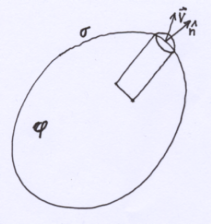
\includegraphics[width=0.6\textwidth]{liouville.png}
%  \caption{Il teorema di Liouville}
%  \label{fig:liouville}
%\end{figure}
%%%%%%%%%%%%%%%%%%%%%%%%%%%%%%%%%%%%%%%%%%%%%%%%%%%%%%%%%%%

Il teorema di Lioville stabilisce che la densità $\rho(q,p;t)$ si comporta come un {\em fluido incomprimibile}. Per vederlo, consideriamo l'evoluzione nel tempo di $\de{\calN}$. Prendiamo un punto rappresentativo $(q,p)$ all'interno del volumetto $\dephi$ al tempo $t$. Dopo in intervallo di tempo $\delta t$ il punto $(q,p)$ si sarà spostato in $(q',p')$, con
\bea
\label{eq:03-spostaqp}
q_i' &=& q_i + \dot{q}_i\delta t + O(\delta t^2) \nonumber \\
p_i' &=& p_i + \dot{p}_i\delta t + O(\delta t^2)
\eea
L'elemento di volume originale, $\dephi$, è un ipercubo. Dopo lo spostamento risulterà distorto, e dobbiamo calcolare il nuovo elemento di volume $\dephi' = \prod_i \de{q_i'}\de{p_i'}$. Possiamo subito scrivere
\bea
\de{q_i'} &=& \de{q_i} + \dpar{\dot{q}_i}{q_i}\de{q_i} \delta t+O(\delta t^2) \nonumber \\
\de{p_i'} &=& \de{p_i} + \dpar{\dot{p}_i}{p_i}\de{p_i} \delta t+O(\delta t^2) \nonumber
\eea
Dalla precedente segue che per ciascuna coppia coniugata abbiamo
\be
\label{eq:03-evolvol}
\de{q_i'}\de{p_i'} = \de{q_i}\de{p_i}\left[
1 + \left(
\dpar{\dot{q}_i}{q_i} + \dpar{\dot{p}_i}{p_i}
\right)\delta t + O(\delta t^2)
\right]
\ee
Le equazioni del moto (\ref{eq:03-eqmotoH}) ci dicono però che
\be
\dpar{\dot{q}_i}{q_i} = \dfrac{\partial}{\partial q_i}\dpar{\Ham}{p_i}
= \dfrac{\partial^2\Ham}{\partial q_i\partial p_i}
\ee
e che
\be
\dpar{\dot{p}_i}{p_i} = -\dfrac{\partial}{\partial p_i}\dpar{\Ham}{q_i}
= -\dfrac{\partial^2\Ham}{\partial q_i\partial p_i}
\ee
Il termine proporzionale a $\delta t$ nella (\ref{eq:03-evolvol}) si annulla dunque per le equazioni del moto, e otteniamo $\dephi' = \dephi$. Questo significa che tutti i punti rappresentativi $\de{\calN}$ originariamente vicini al punto $(q,p)$ vengono trasportati nelle immediate vicinanze di $(q',p')$ in modo tale da preservare il volume occupato. Il rapporto $\de{\calN}/\dephi$ rimane invariato, che è un altro modo di dire che $\rho$ si comporta come  un fluido incomprimibile.

Introducendo le parentesi di Poisson
\be
\label{eq:03-parentesi-poisson}
\{\rho,\Ham\} = \sum_{i}\left( \dpar{\rho}{q_{i}}\dpar{\Ham}{p_{i}} - \dpar{\rho}{p_{i}}\dpar{\Ham}{q_{i}} \right)
\ee
la condizione di incomprimibilità, $\rho(q',p';t+\de{t}) = \rho(q,p;t)$ può finalmente essere scritta, in forma differenziale, in questo modo:
\be
\label{eq:03-liouville}
\dfrac{\de{\rho}}{\de{t}} = \dpar{\rho}{t} + \{\rho,\Ham\} = 0
\ee
che è appunto il {\em teorema di Liouville}.

Ricordiamo ora che siamo interessati alla descrizione di sistemi macroscopici all'equilibrio; il valore d'aspettazione di qualsiasi osservabile deve essere costante nel tempo, o meglio, indipendente dal tempo. In questo caso abbiamo che $\rho$ stessa non può dipendere esplicitamente dal tempo; dobbiamo certamente imporre, come primo passo, la condizione di stazionarietà:
\be
\dpar{\rho}{t} = 0
\ee
A questo punto siamo costretti anche a chiedere che le parentesi di Poisson si annullino:
\be
\label{eq:03-parpois0}
\{\rho,\Ham\} = 0
\ee
Si vede subito che $\rho$ non può essere un'arbitraria funzione di $(q,p)$, ma dev'essere una funzione dell'hamiltoniana del sistema. Il modo più semplice di implementare la condizione (\ref{eq:03-parpois0}) è quella di assumere $\rho$ costante sulla ipersuperficie a energia costante $E$ nello spazio delle fasi. Ciò corrisponde a considerare l'\ensemble\ micronanonico.

%%%%%%%%%%%%%%%%%%%%%%%%%%%%%%%%%%%%%%%%%%%%%%%%%%%%%%%%%%%%%%%%%%%%%%%%
\section{L'\ensemble\ microcanonico}
\label{sec:03-micro}
%%%%%%%%%%%%%%%%%%%%%%%%%%%%%%%%%%%%%%%%%%%%%%%%%%%%%%%%%%%%%%%%%%%%%%%%

Consideriamo dunque un sistema fisico in cui le grandezze macroscopiche fondamentali siano il numero di particelle, $N$, il volume $V$ in cui sono racchiuse e l'energia totale $E$ del sistema stesso, che si suppone conservata (sistema isolato). La terna $(N,\,V,\,E)$ rappresenta quindi un macrostato del sistema.

In realtà pensare di tenere l'energia esattamente fissata non è una buona idea; per modellizzare meglio una situazione fisica reale possiamo pensare a un sistema in cui l'energia possa variare di una quantità $\pm \Delta/2$ intorno al valore centrale $E$ (con la condizione naturalmente che $\Delta \ll E$).

La condizione
\be
\Ham(q,p) = E
\ee
definisce una ipersuperficie ($6N-1$ dimensionale) nello spazio delle fasi $\Phi$. Sia ora $\gamma$ il volume nello spazio delle fasi definito dalla condizione
\be
E-\frac{\Delta}{2} \le \Ham \le E+\frac{\Delta}{2}
\ee
ossia il volume del guscio di spessore $\Delta$ intorno alla ipersuperficie a energia costante $E$. L'ensemble microcanonico è definito dalla condizione che $\rho$ sia costante all'interno del volume $\gamma$ e sia nulla all'esterno. Abbiamo dunque
\be
\gamma = \int\limits_{E-\frac{\Delta}{2} \le \Ham \le E+\frac{\Delta}{2}}\dephi
\ee

Con queste definizioni otteniamo, per il valore d'aspettazione di una generica osservabile, l'equazione
\be
\aspetta{A} = \frac{1}{\gamma}\int\limits_\gamma A(q,p)\dephi
\ee

Prima di considerare il numero di microstati $\Gamma$ e il suo rapporto con $\gamma$, è giunto il momento di svelare una drammatica verità: la meccanica statistica classica non è ben fondata. Ciò dovrebbe essere intuitivo: la meccanica statistica ha a che fare col comportamento dei costituenti microscopici di un sistema macroscopico, e nel mondo microscopico valgono le regole quantistiche. Un corretto conto dei microstati può essere effettuato solo col formalismo quantistico. Dunque da un punto di vista logico sarebbe più giusto fondare la meccanica statistica sul formalismo quantistico e poi vedere sotto quali condizioni si può ricavare la meccanica statistica classica. Questo però non è stato il percorso storico, e dal punto di vista didattico è preferibile seguire la stessa strada dei padri fondatori della meccanica statistica.

Dovrebbe essere chiaro che il valore del volume $\gamma$ ha qualcosa a che fare $\Gamma$ ma in ogni caso $\gamma$ non coincide con il numero dei microstati. Per stabilire una corrispondenza numerica precisa occorre trovare un ``volume fondamentale'' $\gamma_{0}$, il cui significato fisico è il seguente: a un microstato del sistema corrisponde un volume $\gamma_{0}$ nello spazio delle fasi. Avremo dunque
\be
\Gamma = \gamma/\gamma_{0}
\ee
e quindi
\be
S = k \ln(\gamma/\gamma_{0})
\ee
Tutto ciò dovrebbe essere intuitivo: infatti da un punto di vista quantistico l'idea di {\em punto rappresentativo} nello spazio delle fasi perde senso, perché a causa delle relazioni di indeterminazione di Heisemberg non possiamo specificare con precisione arbitraria sia la posizione $q$ sia il momento $p$ di una particella. Il meglio che possiamo fare è quello di assumere che il punto divenga, appunto, un volumetto $\gamma_0$.

Il problema è dunque quello di trovare $\gamma_{0}$. Lo faremo servendoci di un ``trucco'': considereremo un paio di sistemi semplici e calcoleremo $\gamma$ nel caso classico (nel quale il volume nello spazio delle fasi ha significato) e $\Gamma$ col formalismo quantistico. Il rapporto tra i due risultati darà il valore di $\gamma_{0}$.

%%%%%%%%%%%%%%%%%%%%%%%%%%%%%%%%%%%%%%%%%%%%%%%%%%%%%%%%%%%%%%%%%%%%%%%%
\subsection{Il gas ideale}
%%%%%%%%%%%%%%%%%%%%%%%%%%%%%%%%%%%%%%%%%%%%%%%%%%%%%%%%%%%%%%%%%%%%%%%%

Abbiamo come al solito $N$ particelle identiche non interagenti racchiuse in un volume $V$. L'hamiltoniana del sistema è
\be
\Ham = \sum_{i=1}^{3N}\frac{p^2_i}{2m}
\ee
in cui $m$ è la massa delle particelle. Abbiamo
\be
\gamma = \int\limits_{E-\frac{\Delta}{2} \le \Ham \le E+\frac{\Delta}{2}}\dephi
\ee
L'integrazione sulle coordinate dà semplicemente un fattore $V^{N}$ perché l'Hamiltoniana non dipende dalle coordinate ma solo dai momenti. Abbiamo dunque
\be
\gamma = V^N\int\limits_{2m(E-\Delta/2)\le\sum_i p_{i}^{2}\le 2m(E+\Delta/2)}\de^{3N} p
\ee
$\gamma$ rappresenta il volume di un iperguscio confinato tra due ipersfere di raggi rispettivamente $\sqrt{2m(E-\Delta/2)}$ (raggio interno) e $\sqrt{2m(E+\Delta/2)}$ (raggio esterno). Per $\Delta \ll E$ possiamo scrivere $\sqrt{2m(E\pm\Delta/2)}\simeq\sqrt{2mE}(1\pm\Delta/4E)$ e lo spessore del guscio risulta quindi pari a $R_{+}-R_{-}\simeq\Delta\sqrt{m/2E}$. Moltiplicando questo valore per la superficie dell'ipersfera di raggio $\sqrt{2mE}$ otteniamo con buona approssimazione il volume del guscio. Utilizzando il risultato per la superficie di un'ipersfera in $n$ dimensioni, ossia
\be
S_{n}(R) = \frac{2\pi^{n/2}}{\Gamma(n/2)}R^{n-1}
\ee
otteniamo, considerando che $n = 3N$:
\be
\gamma \simeq \frac{\Delta}{E}V^{N}\frac{(2\pi mE)^{3N/2}}{(3N/2 - 1)!}
\ee
Nel caso quantistico avevamo ottenuto (vedi capitolo precedente)
\be
\Gamma \simeq \frac{\Delta}{E}\frac{V^{N}}{h^{3N}}\frac{(2\pi mE)^{3N/2}}{(3N/2 - 1)!}
\ee
e dal confronto otteniamo subito
\be
\gamma_{0}\equiv(\gamma/\Gamma) = h^{3N}
\ee
Notiamo che dal punto di vista dimensionale le cose tornano: il prodotto di una posizione $q$ per un momento $p$ dà un oggetto che ha le dimensioni di un momento angolare, e $\gamma_0$ deve proprio avere le dimensioni di un momento angolare alla $3N$

%%%%%%%%%%%%%%%%%%%%%%%%%%%%%%%%%%%%%%%%%%%%%%%%%%%%%%%%%%%%%%%%%%%%%%%%
\subsection{L'oscillatore armonico}
%%%%%%%%%%%%%%%%%%%%%%%%%%%%%%%%%%%%%%%%%%%%%%%%%%%%%%%%%%%%%%%%%%%%%%%%

Consideriamo un oscillatore armonico unidimensionale; l'hamiltoniana del sistema è
\be
\Ham = \frac{1}{2m}p^2 + \frac{1}{2}m\omega^2 q^2
\ee
La soluzione delle equazioni del moto ci fornisce il risultato
\bea
\label{eq:03-oat}
q &=& \phantom{-m\omega} A\cos(\omega t + \phi)\nonumber\\
p &=&           -m\omega A\sin(\omega t + \phi)
\eea
in cui $A$ è l'ampiezza dell'oscillazione e $\phi$ una fase. L'energia del sistema è pari a
\be
E = \frac{1}{2}m\omega^2 A^2 = \mbox{\textrm costante}
\ee
Per ottenere la traiettoria nello spazio delle fasi occorre eliminare il tempo dalle \ref{eq:03-oat}. Si ottiene facilmente
\be
\frac{m\omega^2 q^2}{2E} + \frac{p^2}{2mE} = 1
\ee
Riconosciamo immediatamente l'equazione di un'ellisse di area $2\pi E/\omega$. Se ora consideriamo un oscillatore con energia $E+\Delta/2$ e un altro con energia $E-\Delta/2$ otteniamo subito che l'area del guscio racchiuso tra le due ellissi è pari a
\be
\gamma = \frac{2\pi\Delta}{\omega}
\ee

Consideriamo ora la situazione quantistica: gli autovalori dell'energia sono quantizzati,
\be
E_n = (n+\frac{1}{2})\hbar\omega\quad n = 0, 1, 2\dots
\ee
e se assumiamo di essere in un caso semiclassico, cioè $\hbar\omega \ll \Delta \ll E$, il numero di autostati che hanno un'energia compresa nell'intervallo $(E-\Delta/2\,,\,E+\Delta/2)$ è (asintoticamente) pari a
\be
\Gamma = \frac{\Delta}{\hbar\omega}
\ee
Dal confronto otteniamo subito
\be
\gamma_0 = h
\ee

%%%%%%%%%%%%%%%%%%%%%%%%%%%%%%%%%%%%%%%%%%%%%%%%%%%%%%%%%%%%%%%%%%%%%%%%
\subsection{Un sistema di oscillatori armonici}
\label{es:sistoscarm}
%%%%%%%%%%%%%%%%%%%%%%%%%%%%%%%%%%%%%%%%%%%%%%%%%%%%%%%%%%%%%%%%%%%%%%%%

Consideriamo ora un sistema di $N$ oscillatori armonici non interagenti, con frequenza comune pari a $\omega$. Abbiamo
\be
\Ham = \sum_{i=1}^N \left[\frac{1}{2m}p^2_i + \frac{1}{2}m\omega^2q_i^2\right]
\ee
Sia $E$ l'energia totale del sistema. Calcoliamo ora il volume dello spazio delle fasi racchiuso dall'ipersuperficie a energia costante $E$:
\be
\Sigma(E) = \int\limits_{\sum_i(p_i^2/2m+m\omega^2q_i^2/2) \le E} \de^N q \de^N p
\ee
Poniamo
\bea
x_i     &=& \sqrt{\frac{m\omega^2}{2}}\;q_i\nonumber\\
x_{i+N} &=& \sqrt{\frac{1}{2m}}\;p_i
\eea
ottenendo
\be
\Sigma(E) = \left(\frac{2}{\omega}\right)^N\int\limits_{\sum_i x_i^2 \le E}\de^{2N}x
\ee
Sfruttiamo il risultato noto per il volume di un'ipersfera in $n$ dimensioni,
\be
V_n(R) = \frac{\pi^{n/2}}{(n/2)!}R^n
\ee
ottenendo subito
\be
\Sigma(E) = \frac{1}{N!}\left(\frac{2\pi}{\omega}E\right)^N
\ee
Per il calcolo della quantità che ci interessa, ossia il volume $\Gamma$ del guscio di spessore $\Delta$ intorno alla ipersuperficie di energia costante $E$, abbiamo come al solito
\be
\Gamma = \Delta\dpar{\Sigma(E)}{E} = \left(\frac{2\pi}{\omega}\right)^N\frac{\Delta}{(N-1)!}E^{N-1}
\ee

Passiamo ora al calcolo quantistico. Per il $k$-mo oscillatore avremo
\be
\epsilon_k = \left(n_k+\frac{1}{2}\right)\hbar\omega
\ee
e per l'energia totale del sistema
\be
E = \sum_{k=1}^N\epsilon_k = \frac{N\hbar\omega}{2} + \hbar\omega\sum_k n_k
\ee
Tenere fissata l'energia $E$ equivale a tenere fissato il numero intero
\be
\label{eq:03-Rpalline}
R \equiv \frac{E}{\hbar\omega} - \frac{N}{2} = \sum_k n_k
\ee
dunque ora il problema è capire come riuscire a ottenere il numero di modi in cui posso distribuire gli $N$ oscillatori sui vari livelli in modo che $R$ rimanga costante. Ricorriamo a un trucco (vedi figura \ref{fig:03-scapal}): immaginiamo di avere $N$ contenitori, che stilizziamo con $N+1$ stanghette verticali e $R$ palline. I contenitori rappresentano gli $N$ oscillatori, mentre il numero di palline nel contenitore $k$--mo rappresenta il numero $n_k$. Il numero totale $R$ di palline rappresenta ovviamente l'energia scritta come nell'eq.(\ref{eq:03-Rpalline}). Dentro al primo contenitore mettiamo $n_1$ palline, nel secondo $n_2$ palline e così via. Per calcolare in quanti modi posso disporre le palline nei contenitori, ossia in quanti modi possiamo realizzare il set dei numeri d'occupazione dei vari livelli, $\{n_k\}$, in modo che la somma sia uguale a $R$, basta considerare tutte le permutazioni possibili di $N-1$ stanghette (le 2 alle estremità sono fissate) e $R$ palline, e poi tener conto che stanghette sono indistinguibili e così pure le palline.
%%%%%%%%%%%%%%%%%%%%%%%%%%%%%%%%%%%%%%%%%%%%%%%%%%%%%%%%%%%%%%%%%%%%%%%%%
\begin{figure}[!ht]
  \centering
  \begin{tikzpicture}
  \draw[very thick] (0.0,0.0) -- (0.0,2.0);
  \draw (2.0,0.0) -- (2.0,2.0);
  \draw (4.0,0.0) -- (4.0,2.0);
  \draw (6.0,0.0) -- (6.0,2.0);
  \draw (9.0,0.0) -- (9.0,2.0);
  \draw[very thick] (11.0,0.0) -- (11.0,2.0);
  
  \draw[dotted] (7.0,1.0) -- (8.0,1.0);
  
  \shade[ball color=blue] (0.5,1.0)  circle (.15cm);
  \shade[ball color=blue] (1.5,1.0)  circle (.15cm);
  \shade[ball color=blue] (4.5,1.0)  circle (.15cm);
  \shade[ball color=blue] (5.0,1.0)  circle (.15cm);
  \shade[ball color=blue] (5.5,1.0)  circle (.15cm);
  \shade[ball color=blue] (10.0,1.0) circle (.15cm);
 
  \draw [red!80!black](0.01,2.3)  node{$1$};
  \draw [red!80!black](2.01,2.3)  node{$2$};
  \draw [red!80!black](4.01,2.3)  node{$3$};
  \draw [red!80!black](6.01,2.3)  node{$4$};
  \draw [red!80!black](9.01,2.3)  node{$N$};
  \draw [red!80!black](11.01,2.3) node{$N+1$};

  \draw [blue!80!black](0.51,0.6)  node{$1$};
  \draw [blue!80!black](1.51,0.6)  node{$2$};
  \draw [blue!80!black](4.51,0.6)  node{$3$};
  \draw [blue!80!black](5.01,0.6)  node{$4$};
  \draw [blue!80!black](5.51,0.6)  node{$5$};
  \draw [blue!80!black](10.01,0.6) node{$R$};
\end{tikzpicture}

  \caption{Conteggio degli stati come permutazione tra $N-1$ linee e $R$ palline. La prima e l'ultima linea, in grassetto, sono fisse e non soggette a permutazione. La prima scatola (cioè il primo oscillatore) contiene $2$ palline (il primo oscillatore è sul secondo livello di energia). La seconda scatola nessuna pallina (il secondo oscillatore è nel {\em ground--state}). La terza scatola contiene $3$ palline, e così via. L'ultima scatola contiene solo una pallina.}
  \label{fig:03-scapal}
\end{figure}
%%%%%%%%%%%%%%%%%%%%%%%%%%%%%%%%%%%%%%%%%%%%%%%%%%%%%%%%%%%%%%%%%%%%%%%%%

Otteniamo dunque
\be
W = \frac{(N-1+R)!}{(N-1)!R!} \simeq \frac{(N+R)!}{(N)!R!}
\ee
in cui nell'ultimo passaggio abbiamo considerato che $N$ e $R$ sono molto maggiori di $1$. Come nel caso dell'oscillatore singolo ci mettiamo in una situazione semiclassica, ossia valori dell'energia dei singoli oscillatori molto grandi rispetto a $\hbar\omega$. Questo corrisponde a dire che $R \gg N$, e possiamo quindi scrivere
\be
W = \frac{1}{N!}\frac{(R+N)(R+N-1)(R+N-2)\cdots(R+1)R!}{R!} \simeq \frac{R^N}{N!}
\ee
Se ora consideriamo il solito guscio di spessore $\Delta$ intorno all'energia $E$ otteniamo:
\bea
R_+ &=& \left(E+\frac{\Delta}{2}-\frac{N\hbar\omega}{2}\right)\frac{1}{\hbar\omega}\nonumber\\
R_- &=& \left(E-\frac{\Delta}{2}-\frac{N\hbar\omega}{2}\right)\frac{1}{\hbar\omega}
\eea
e otteniamo subito
\bea
\Gamma &=& \frac{1}{N!}(R_+-R_-)\nonumber\\
       &=& \frac{1}{N!}\frac{E^N}{(\hbar\omega)^N}\left[\left(1+\frac{\Delta-N\hbar\omega}{2E}\right)^N -
       \left(1-\frac{\Delta+N\hbar\omega}{2E}\right)^N\right]
\eea
e usando lo sviluppo $(1\pm x)^n\simeq 1\pm nx$ otteniamo subito
\be
\Gamma = \frac{\Delta E^{N-1}}{(N-1)!(\hbar\omega)^N}
\ee
e dal confronto con l'espressione per $\gamma$ troviamo immediatamente
\be
\gamma_0 = h^N
\ee

%%%%%%%%%%%%%%%%%%%%%%%%%%%%%%%%%%%%%%%%%%%%%%%%%%%%%%%%%%%%%%%%%%%%%%%%
\subsection{La regola generale}
%%%%%%%%%%%%%%%%%%%%%%%%%%%%%%%%%%%%%%%%%%%%%%%%%%%%%%%%%%%%%%%%%%%%%%%%

I tre esempi appena visti ci lasciano intuire la regola generale, che è questa: per ottenere il numero di microstati per un sistema classico con $M$ gradi di libertà totali con volume microcanonico $\gamma$ nello spazio delle fasi, occorre dividere $\gamma$ per $h^M$.

Ricordiamo che in ogni caso il vero conteggio del numero dei microstati dovrebbe essere ottenuto con il formalismo quantistico. Il fattore di conversione $h^M$ può essere compreso intuitivamente considerando le relazioni di indeterminazione di Heisenberg: se pensiamo a un sistema unidimensionale con una sola particella è chiaro che a livello quantistico non possiamo determinare contemporaneamente e con posizione arbitraria posizione e momento della particella, ma abbiamo, al meglio
\be
\delta q \delta p \sim \hbar
\ee
Dunque un particolare microstato del sistema occupa, nello spazio delle fasi, un volumetto di ordine $h$. Il risultato si generalizza subito a sistemi con $M$ gradi di libertà.

%%%%%%%%%%%%%%%%%%%%%%%%%%%%%%%%%%%%%%%%%%%%%%%%%%%%%%%%%%%%%%%%%%%%%%%%
\section{Esercizi per il Capitolo \ref{cap:elementi}}
%%%%%%%%%%%%%%%%%%%%%%%%%%%%%%%%%%%%%%%%%%%%%%%%%%%%%%%%%%%%%%%%%%%%%%%%

%-----------------------------------------------------------------------
% ESERCIZIO ULTRARELATIVISTICO
%-----------------------------------------------------------------------
\begin{Exercise}[title={Gas ideale ultrarelativistico},label={ex:03-gicur}]
Si consideri un gas ideale composto da $N$ particelle ultrarelativistiche racchiuse in un volume $V$. Sia $E$ l'energia totale del sistema, con $E = \mathrm{costante}$. Si calcoli, col formalismo microcanonico, la relazione che lega la pressione all'energia. Si dimostri inoltre che nel caso ultrarelativistico
\be
\gamma\equiv C_P/C_V = 4/3\nonumber
\ee
\end{Exercise}

%-----------------------------------------------------------------------
% ESERCIZIO OSCILLATORI DI FERMI
%-----------------------------------------------------------------------
\begin{Exercise}[title={Oscillatori di Fermi},label={ex:03-oscfermi}]
Si consideri un sistema composto da $N$ ``particelle'' non interagenti e distinguibili, ognuna delle quali può stare in due livelli di energia, $\pm\varepsilon$. Sia $E$ l'energia (fissata) del sistema. Si ricavi la temperatura microcanonica d'equilibrio $T$ e si calcoli il numero d'occupazione medio dei due livelli in funzione della temperatura $T$, discutendo i limiti $T\to 0$ e $T\to\infty$.
Si calcoli inoltre l'entropia $S$ come funzione dell'energia $E$, discutendo il comportamento di $S$ per $E > 0$: cosa implica, per la temperatura $T$, che $E$ sia maggiore di zero?
\end{Exercise}

\newpage

%-----------------------------------------------------------------------
% ESERCIZIO OSCILLATORI DI FERMI CON DEGENERAZIONE
%-----------------------------------------------------------------------
\begin{Exercise}[title={Sistema a due livelli con degenerazione},label={ex:03-quasioscfermi}]
Si consideri un sistema di $N$ particelle identiche ma distinguibili e non interagenti. Il sistema ammette due livelli di energia di singola particella: $E_0 = 0$ e $E_1 = \varepsilon > 0$.
Il livello di energia $E_1$ è $g$-degenere mentre il livello $E_0$ è non degenere.
Sia $E = n_1\varepsilon$ l'energia totale del sistema ($n_1$ è il numero medio di particelle sul livello di energia $E_1$).
\begin{enumerate}
  \item Usando il formalismo dell'ensemble microcanonico trovare il numero di occupazione $n_1$ (per le particelle nel livello a energia $E_1$) e $n_0$ (per le particelle nel livello a energia $E_0$) in funzione della temperatura d'equilibrio $T$.
  \item Si consideri il caso in cui $g=2$. Se il sistema ha energia $E=0.75\,N\varepsilon$ ed è posto in contatto termico con una riserva termica a temperatura costante $T= 500\,K$, in che direzione fluisce il calore?
\end{enumerate}
\end{Exercise}

%-----------------------------------------------------------------------
% ESERCIZIO SPIN 1
%-----------------------------------------------------------------------
\begin{Exercise}[title={Particelle di spin 1}, label={ex:03-spin1}]
Si consideri un sistema composto da $N$ particelle non--interagenti e indistinguibili. L'hamiltoniana totale del sistema è
\be
\Ham = -h\sum_{i=1}^N \sigma_i \quad\quad \sigma_i = -1, 0, 1
\ee
dove $h$ una costante con le dimensioni di un'energia. Si può immaginare che le particelle abbiano spin $1$, quindi un certo momento magnetico in direzione $z$, e che $h$ sia il prodotto scalare di un campo magnetico esterno per il momento magnetico delle particelle.

Sia $E$ l'energia, fissata, del sistema. Chiamando $N_\sigma$ il numero d'occupazione del livello $\sigma$, con $\sigma = -1, 0, 1$, si calcoli, utilizzando il formalismo microcanonico, il rapporto $N_{-1}/N_{1}$ in funzione della temperatura $T$ d'equilibrio. Si calcoli inoltre $A(N,T)$, l'energia libera di von Helmholtz.

Si confronti il risultato con quello ottenuto utilizzando il formalismo canonico (vedi Capitolo \ref{cap:canonico}).
\end{Exercise}

%-----------------------------------------------------------------------
% ESERCIZIO MOLECOLE DIATOMICHE CON TRE ORIENTAZIONI
%-----------------------------------------------------------------------
\begin{Exercise}[title={Particelle diatomiche},label={ex:04-diatom}]
 Consideriamo superficie metallica bidimensionale e quadrata su cui sono vincolate $N$ molecole diatomiche. Ogni molecola può giacere sulla superficie e avere, in questo caso, solo due orientazioni possibili, lungo $x$ o lungo $y$, oppure può essere diretta lungo l'asse $z$, perpendicolare alla superficie. Il costo energetico associato all'allineamento lungo l'asse $z$ è $\varepsilon > 0$,  mentre quello associato all'allineamento lungo $x$ o $y$ e nullo.
\begin{enumerate}
\item Quanti sono i microstati che generano rispettivamente il macrostato a energia minima e a energia massima?
\item  Fissato il macrostato ad energia $E$, calcolare l'entropia $S(E, N )$ del sistema.
\item Calcolare il calore specifico $C(T )$ e disegnarne l'andamento in funzione di $T$.
\item Qual è la probabilità che le molecole siano allineate lungo $z$?
\item Qual è il valore più probabile che può assumere l'energia interna per ogni $T>0$?
\end{enumerate}

\end{Exercise}

%%%%%%%%%%%%%%%%%%%%%%%%%%%%%%%%%%%%%%%%%%%%%%%%%%%%%%%%%%%%%%%%%%%%%%

\vskip 0.75cm
\begin{flushright}
{\em Ultimo aggiornamento del Capitolo: 22.04.2017}
\end{flushright}

%%%%%%%%%%%%%%%%%%%%%%%%%%%%%%%%%%%%%%%%%%%%%%%%%%%%%%%%%%%%%%%%%%%%%%%%
\chapter{L'\ensemble\ canonico}
\label{cap:canonico}
%%%%%%%%%%%%%%%%%%%%%%%%%%%%%%%%%%%%%%%%%%%%%%%%%%%%%%%%%%%%%%%%%%%%%%%%

Per molte ottime ragioni considerare esattamente fissata l'energia di un sistema fisico non è una buona idea. {\em In primis} occorre notare che una misura diretta ed esatta dell'energia interna di un sistema termodinamico è a tutti gli effetti pratici impossibile (in genere l'energia è ricavata indirettamente, da misure di altre osservabili fisiche). In secondo luogo sappiamo bene che misurando un'osservabile qualsiasi di un sistema fisico perturbiamo il sistema stesso. \`E vero che almeno classicamente possiamo pensare di rendere trascurabile la perturbazione dovuta alla misura ma è anche vero che in ultima analisi stiamo considerando la fisica dei costituenti elementari di un corpo macroscopico: come abbiamo già avuto occasione di notare, tali costituenti elementari obbediranno alle leggi quantistiche. Poco male, diranno subito i miei piccoli lettori: possiamo, come abbiamo già fatto, assumere che l'energia fluttui intorno al valore $E$ di una quantità $\Delta$. La risposta a questa obiezione è duplice: da una parte, la fluttuazione $\Delta$ è (quasi) completamente arbitraria, e la sua comparsa nei calcoli dovrebbe essere evitata; dall'altra, $\Delta$ non può essere completamente arbitrario, come abbiamo visto; in particolare non può andare a $0$ nel limite termodinamico, pena la comparsa di divergenze in quantità fisiche. Solo il rapporto $\Delta/E$ deve andare a zero. (Di fatto che la meccanica statistica {\em classica} funzioni è alla fin fine solo un miracolo d'equilibrismo).

Possiamo pensare di tenere costante qualcos'altro, al posto dell'energia? La risposta è ovviamente sì. La relazione tra temperatura ed energia delle molecole di un gas ideale, nella teoria cinetica, ci suggerisce che potremmo tenere costante la temperatura $T$ e lasciare che l'energia possa liberamente fluttuare. In pratica consideriamo macrostati che non sono più caratterizzati dalla terna $(N\,,\,V\,,E)$ ma dalla terna $(N\,,\,V\,,T)$. Come vedremo  presto, la sorprendente risposta a questa richiesta è che di fatto non cambia niente.

%%%%%%%%%%%%%%%%%%%%%%%%%%%%%%%%%%%%%%%%%%%%%%%%%%%%%%%%%%%%%%%%%%%%%%%%
\section{Sistema all'equilibrio con una riserva termica}
\label{sec:04-equilibrio}
%%%%%%%%%%%%%%%%%%%%%%%%%%%%%%%%%%%%%%%%%%%%%%%%%%%%%%%%%%%%%%%%%%%%%%%%

Immaginiamo che il nostro sistema fisico sia in contatto termico con una riserva, ossia un sistema molto più grande (al limite, l'intero Universo). L'energia del sistema totale è conservata, e sarà uguale alla somma delle energie dei due sistemi:
\be
E_0 = E_r + E'_r
\ee
in cui $E_r$ è l'energia del nostro sistema fisico ed $E'_r$ l'energia della riserva termica. Notiamo che i due sistemi, essendo in contatto termico e all'equilibrio, avranno una temperatura comune, $T$, ma in ogni caso l'energia di ciascuno potrà variare tra $0$ e $E_0$, fermo restando il fatto che la loro somma deve rimanere costante. La riserva termica serve a garantire che il sistema fisico che stiamo considerando resti a temperatura costante $T$. Ora, poiché la riserva termica è molto più grande del nostro sistema, possiamo tranquillamente chiedere che in ogni istante di tempo debba valere
\be
\label{eq:04-cond1}
E_r \ll E'_r
\ee
e quindi $E'_r$ sarà sempre molto vicina a $E_0$; a tutti gli effetti pratici possiamo considerare la riserva come un sistema con un'energia fissata, e trattarla quindi con i metodi microcanonici.
Chiamiamo $\Omega'(E'_r)$ il numero dei microstati della riserva termica compatibili con l'energia $E'_r$; risulterà chiaro che più grande $\Omega'(E'_r)$, più grande la probabilità che il sistema fisico abbia energia $E_r$. Se inoltre si considera che tutti i microstati compatibili con $E'_r$ sono ugualmente probabili si arriva alla conclusione che la probabilità $P_r$ di osservare un'energia $E_r$ nel sistema fisico è direttamente proporzionale a $\Omega'(E'_r)$ stesso.

Tenendo conto della (\ref{eq:04-cond1}) possiamo espandere intorno al caso $E_r \simeq 0$:
\be
\ln\Omega'(E'_r) = \ln\Omega'(E_0) + E_r\dpar{\ln\Omega'}{E'_r} + \cdots \simeq \mbox{\textrm{cost}} - \beta'E_r
\ee
e ricordando che all'equilibrio $\beta' = \beta \equiv 1/kT$ otteniamo subito
\be
P_r \propto e^{-\beta E_r}
\ee
Per normalizzare richiediamo che la probabilità totale sia uguale a $1$, e abbiamo quindi
\be
P_r = \frac{e^{-\beta E_r}}{\sum_s e^{-\beta E_s}}
\ee

%%%%%%%%%%%%%%%%%%%%%%%%%%%%%%%%%%%%%%%%%%%%%%%%%%%%%%%%%%%%%%%%%%%%%%%%
\section{L'\ensemble\ canonico}
\label{sec:04-ensemble}
%%%%%%%%%%%%%%%%%%%%%%%%%%%%%%%%%%%%%%%%%%%%%%%%%%%%%%%%%%%%%%%%%%%%%%%%

Consideriamo un \ensemble\ di $\calN$ copie mentali dello stesso sistema fisico; $n_k$ rappresenta il numero di copie con energia $E_k$. L'energia totale dell'\ensemble, ossia la somma di tutte le energie dei sistemi nell'\ensemble, vale $\calE$. Naturalmente $E_k$ e $n_k$ devono soddisfare i vincoli
\bea
\label{eq:04-condcan}
\sum_{k}n_k      &=& \calN\nonumber\\
\sum_{k} E_k n_k &=& \calE \equiv U\calN
\eea
in cui $U$ è l'energia media dell'\ensemble\ che coincide proprio con l'energia interna del sistema fisico originale.
Qualsiasi insieme $\nkset$ che soddisfi i vincoli (\ref{eq:04-condcan}) rappresenta un modo possibile di distribuire l'energia $\calE$ tra gli $\calN$ membri dell'\ensemble. Inoltre ognuno di questi modi possibili può essere ottenuto in molti modi diversi, perché possiamo sempre pensare di permutare i sistemi: per esempio potremmo prendere un sistema con energia $E_1$ e scambiarlo con un sistema con energia $E_5$, ottenendo un altro modo possibile di avere lo stesso set $\nkset$. Chiamiamo $\Wnk$ il numero di modi in cui possiamo ottenere il set $\nkset$:
\be
\label{eq:04-W}
\Wnk = \frac{\calN!}{n_0!n_1!n_2!\cdots}
\ee
Considerando che tutti i possibili stati dell'\ensemble\ compatibili con le (\ref{eq:04-condcan}) hanno la stessa probabilità di occorrere, la frequenza con cui apparirà un determinato insieme
$\nkset$ sarà proporzionale a $\Wnk$

Il nostro obiettivo è quello di calcolare la probabilità $P_k$ di trovare uno degli elementi dell'\ensemble\ in uno stato con energia $E_k$; naturalmente avremo
\be
P_k = \frac{\aspetta{n_k}}{\calN}
\ee
in cui per definizione di media sull'\ensemble\ avremo
\be
\label{eq:04-nrmean}
\aspetta{n_k} = \frac{\sum_{\nkset}'n_k \Wnk}{\sum_{\nkset}' \Wnk}
\ee
e l'apice sulle sommatorie serve a ricordare che le sommatorie stesse devono essere fatte rispettando i vincoli (\ref{eq:04-condcan}). Possiamo anche cercare l'insieme $\nkset$ più probabile, $n_k^*$; come vedremo, nel limite $\calN\to\infty$ i due risultati coincidono. Cominciamo quindi la derivazione dell'\ensemble\ canonico con il metodo del valore più probabile.

%%%%%%%%%%%%%%%%%%%%%%%%%%%%%%%%%%%%%%%%%%%%%%%%%%%%%%%%%%%%%%%%%%%%%%%%
\subsection{Il metodo del valore più probabile}
%%%%%%%%%%%%%%%%%%%%%%%%%%%%%%%%%%%%%%%%%%%%%%%%%%%%%%%%%%%%%%%%%%%%%%%%

L'insieme $n_k^*$ sarà tale da massimizzare $\Wnk$. Come al solito lavoriamo con il logaritmo e assumiamo che $n_k\gg 1$ per ogni $k$:
\be
\label{eq:04-lnW}
\ln W = \ln(\calN!) - \sum_k\ln(n_k!) \simeq \calN\ln\calN - \sum_k n_k\ln n_k
\ee
in cui nell'ultimo passaggio abbiamo usato la formula di Stirling. Se adesso passiamo da $\nkset$ a un insieme leggermente diverso, $\dnkset$, l'espressione (\ref{eq:04-lnW}) cambierà di una quantità
\be
\delta(\ln W) = -\sum_k(\ln n_k + 1)\delta n_k
\ee
e se il set $\nkset$ è quello più probabile allora $\delta(\ln W) = 0$. A causa dei vincoli (\ref{eq:04-condcan}) le variazioni $\delta n_k$ non possono essere arbitrarie, ma devono a loro volta sottostare ai vincoli
\bea
\sum_k \delta n_k     &=& 0\nonumber\\
\sum_k E_k \delta n_k &=& 0
\eea
Il set $n_k^*$ viene quindi calcolato usando il metodo dei moltiplicatori di Lagrange; la condizione che determina $n_k^*$ è
\be
\sum_k[-(\ln n_k^* + 1) - \alpha - \beta E_k]\delta n_k = 0
\ee
Grazie ai moltiplicatori le variazioni $\delta n_k$ sono diventate indipendenti e completamente arbitrarie; perché la somma sia nulla devono quindi essere nulli tutti i coefficienti:
\be
\ln n_k^* = -(\alpha+1) - \beta E_k
\ee
e cioè
\be
n_k^* = C\exp(-\beta E_k)
\ee
in cui $\alpha$ è stato riassorbito nella costante di normalizzazione $C$.
Poiché interpretiamo $n_k^*/\calN$ come la probabilità di trovare un elemento dell'\ensemble\  con energia $E_k$, $C$ scompare con l'ovvia normalizzazione
\be
\frac{n_k^*}{\calN} = \frac{\exp(-\beta E_k)}{\sum_r\exp(-\beta E_r)}
\ee
mentre il parametro $\beta$ è la soluzione dell'equazione
\be
\frac{\calE}{\calN} = U = \frac{\sum_k E_k\exp(-\beta E_k)}{\sum_k \exp(-\beta E_k)}
\ee
Come vedremo in seguito, è naturale identificare ancora una volta $\beta$ con l'inverso di $kT$.

%%%%%%%%%%%%%%%%%%%%%%%%%%%%%%%%%%%%%%%%%%%%%%%%%%%%%%%%%%%%%%%%%%%%%%%%
\subsection{Il metodo di Darwin--Fowler}
%%%%%%%%%%%%%%%%%%%%%%%%%%%%%%%%%%%%%%%%%%%%%%%%%%%%%%%%%%%%%%%%%%%%%%%%

Il nostro obiettivo è ora quello di calcolare $\aspetta{n_k}$; vedi eq. (\ref{eq:04-nrmean}). Per prima cosa introduciamo dei parametri reali $w_k$ e definiamo la funzione
\be
\widetilde{W}\nkset = \Wnk w_0^{n_0} w_1^{n_1} w_2^{n_2}\dots
\ee
Introduciamo ora
\be
\label{eq:04-gamnu}
\Gamma(\calN,U) \equiv \sum_{\nkset}''\widetilde{W}\nkset
\ee
dove si nota che la sommatoria è ancora sottoposta ai vincoli (\ref{eq:04-condcan}). Il motivo per cui si è scelto di indicare i vincoli con due apici sarà chiaro tra poco. La definizione (\ref{eq:04-gamnu}) ci permette di scrivere
\be
\aspetta{n_k} = w_k\dpar{}{w_k}\ln\Gamma(\calN,U)|_{w_r = 1\;\;\forall\;\;r}
\ee
Dalla definizione di $\widetilde{W}\nkset$ abbiamo subito che
\be
\label{eq:04-gamnu2}
\Gamma(\calN,U) \equiv \sum_{\nkset}''\calN!\frac{w_0^{n_0}}{n_0!}
\frac{w_1^{n_1}}{n_1!}\frac{w_2^{n_2}}{n_2!}\cdots
\ee
Ora, se non ci fosse il secondo dei vincoli (\ref{eq:04-condcan}) ma solo il primo, potremmo calcolare $\Gamma(\calN,U)$ al volo, applicando banalmente il teorema multinomiale (vedi sezione (\ref{subsec:app1-multinomiale}) dell'Appendice \ref{app:matematica}):
\be
\Gamma(\calN,U) = (w_0 + w_1 + w_2 + \cdots)^\calN
\ee
Per poter ricavare $\Gamma$ introduciamo un'altra funzione:
\bea
\label{eq:04-gammatilde}
\widetilde{\Gamma}(\calN,U;z) &\equiv& \sum_{\nkset}'\calN!\frac{w_0^{n_0}}{n_0!}
\frac{w_1^{n_1}}{n_1!}\frac{w_2^{n_2}}{n_2!}\cdots z^\calE\nonumber\\
&=& \sum_{\nkset}'\calN!\frac{w_0^{n_0}}{n_0!}
\frac{w_1^{n_1}}{n_1!}\frac{w_2^{n_2}}{n_2!}\cdots z^{n_0E_0 + n_1E_1 + n_2E_2 + \cdots}\nonumber\\
&=& \sum_{\nkset}'\calN!\frac{(w_0 z^{E_0})^{n_0}}{n_0!}
\frac{(w_1 z^{E_1})^{n_1}}{n_1!}\frac{(w_2 z^{E_2})^{n_2}}{n_2!}\cdots
\eea
in cui $z$ è una variabile complessa. Ora l'apice sulla sommatoria è diventato solo uno, per ricordarci che il secondo dei vincoli, quello sull'energia, è caduto: il vincolo sull'energia è stato implementato quando abbiamo scritto esplicitamente, nella (\ref{eq:04-gammatilde}), $z^\calE = z^{n_0E_0+n_1E_1+...}$. Rimane dunque solo il primo vincolo.

A questo punto dobbiamo ricorrere a un trucco. Prima di tutto, poiché l'energia, almeno classicamente, è sempre definita a meno di una costante additiva arbitraria, siamo liberi di porre $E_0 = 0$. Inoltre scegliamo un'unità di misura per l'energia talmente fine da rendere le $E_k$ numeri interi a tutti gli effetti pratici (se si pensa ai livelli di energia quantistici di una particella in una scatola si vede subito che questo è certamente possibile). Inoltre la nostra unità di misura per l'energia è tale che le $E_k$ non hanno nessun divisore comune (questa è un'assunzione che ci servirà in seguito). Per giustificare la fondatezza di quest'ultima assunzione basti pensare che se gli $E_k$ avessero un divisore comune allora anche $\calE$ l'avrebbe, perché altrimenti il secondo dei vincoli (\ref{eq:04-condcan}) non sarebbe soddisfatto. Sia ora $\tau$ il massimo comun divisore: in altre parole posso sempre scrivere
\be
\tau\calE' = \tau\sum_k n_k E_k'
\ee
in cui le variabili primate continuano a essere numeri interi. Se ora divido entrambi i membri per $\tau$ ottengo energie con valori interi senza nessun divisore comune (globale).

Adesso possiamo finalmente applicare il teorema multinomiale e scrivere
\be
\label{eq:04-serie1}
\widetilde{\Gamma}(\calN,U;z) = (w_0 z^{E_0} + w_1 z^{E_1} + w_2 z^{E_2} + \cdots)^\calN \equiv f^\calN(z)
\ee
Ora espandiamo in serie la funzione, scrivendo
\be
\label{eq:04-serie2}
\widetilde{\Gamma}(\calN,U;z) = \sum_n\Gamma_n z^n
\ee
e risulta subito evidente dalla definizione (\ref{eq:04-gammatilde}) che $\Gamma(\calN,U) = \Gamma_{\calE}$ (ricordiamo che $\calE$, con la nuova scala dell'energia, è diventato un numero intero). Per il nostro calcolo dobbiamo quindi solo ricavare il coefficiente $\Gamma_{\calE}$ dell'espansione, e il teorema dei residui ci permette di scrivere
\be
\label{eq:04-residui}
\Gamma(\calN,U) = \frac{1}{2\pi i}\oint\frac{\widetilde{\Gamma}(\calN,U;z)}{z^{\calE+1}}\de z
\ee
La serie (\ref{eq:04-serie2}) ha un raggio di convergenza $\rho$ (quale che sia, $\rho \le 1$). Se si analizza separatamente il comportamento del numeratore e del denominatore della funzione integranda nella (\ref{eq:04-residui}) (vedi figura \ref{fig:04-x0}) ci si rende subito conto che la funzione integranda stessa deve avere, sull'asse reale, un unico minimo per un valore $x_0 < 1$ della parte reale $x$ di $z = x + iy$. Intuitivamente possiamo ragionare così; nella funzione integranda il numeratore parte da $1$ per $z=0$ e va monotonicamente all'infinito positivo verso il bordo di convergenza della serie (\ref{eq:04-serie1}). Il fattore $z^{-\calE-1}$ parte dall'infinito positivo per $z=0$ e decresce monotonicamente verso $0$, conservando un valore finito sul bordo di convergenza della serie (\ref{eq:04-serie1}). Che ci debba essere un minimo in $x_0$, con $0 < x_0 < 1$ è evidente. Per i dettagli della dimostrazione che il minimo è unico si veda \cite{Schr}.
%%%%%%%%%%%%%%%%%%%%%%%%%%%%%%%%%%%%%%%%%%%%%%%%%%%%%%%%%%%%%%%%%%%%%%%%%
\begin{figure}[h]
  \centering
  \begin{tikzpicture}[scale=10]
  \draw[->] (-0.05,0) -- (1.1,0);
  \draw[->] (0,-0.05) -- (0,1);
  \draw[color=red!80!black]  (0.005,0.9) .. controls (0.1,0.1) and (0.5,0.01) .. (0.9,0.005);
  \draw[color=blue!80!black] (0,0.1)     .. controls (0.8,0.2) and (0.99,0.5) .. (0.995,1);
  \draw (0.03,0.8) .. controls (0.2,0.2) and (0.92,0.2) .. (0.98,0.9);
  
  \draw[dotted] (1,0) -- (1,1);
  \draw (1,-0.03) node{$\rho$};
  \draw[dotted] (0.52,0) -- (0.52,0.36);
  \draw (0.52,-0.03) node{$x_0$};
  
  \draw[color=red!80!black] (0.7,0.05) node{$x^{-\mathcal{E}-1}$};
  \draw[color=blue!80!black] (0.7,0.25) node{$f^{\mathcal{N}}(x)$};
\end{tikzpicture}

  \caption{Determinazione di $x_0$}
  \label{fig:04-x0}
\end{figure}
%%%%%%%%%%%%%%%%%%%%%%%%%%%%%%%%%%%%%%%%%%%%%%%%%%%%%%%%%%%%%%%%%%%%%%%%%
Per ottenere la condizione di minimo scriviamo
\be
\frac{f^\calN(z)}{z^{\calE+1}} \equiv e^{\calN g(z)}
\ee
e poiché il circuito chiuso nell'integrale della (\ref{eq:04-residui}) è arbitrario, lo prendiamo essere un cerchio di raggio $x_0$. La condizione di minimo
\be
\frac{\de e^{\calN g(x)}}{\de x} = 0
\ee
diventa subito
\be
\frac{\de g(x)}{\de x} = 0
\ee
con
\be
g(x) = \frac{1}{\calN}(\calN\ln f - (\calN U + 1)\ln x) \simeq \ln f - U\ln x
\ee
in cui nell'ultimo passaggio abbiamo sfruttato il fatto che $\calN U \gg 1$. Abbiamo dunque la condizione
\be
\label{eq:04-condmin}
g'(x_0) = \frac{f'(x_0)}{f(x_0)} - \frac{U}{x_0} = 0
\ee
Teniamo a mente questo risultato: anche nel limite $\calN\to\infty$, il valore di $x_0$ è indipendente da $\calN$. Poi, ricordando che
\be
f(x) = \sum_k w_k x^{E_k}
\ee
otteniamo subito
\be
x_0 f'(x_0) = \sum_k E_k w_k x_0^{E_k}
\ee
e introducendo il parametro $\beta$
\be
x_0 \equiv e^{-\beta}
\ee
dalla (\ref{eq:04-condmin}) possiamo ricavare immediatamente
\be
U = \frac{\sum_k E_k w_k e^{-\beta E_k}}{\sum_k w_k e^{-\beta E_k}}
\ee
\`E da notare che come nel caso del valore più probabile, anche qui $\beta$ lo si ricava dall'equazione precedente, una volta che tutte le $w_k$ siano state poste uguali a 1, come occorre fare alla fine del procedimento.
Dobbiamo ora considerare cosa succede se, partendo da $x_0$, ci spostiamo lungo la direzione immaginaria $y$. Le relazioni di Cauchy--Riemann,
\be
\frac{\partial^2 f}{\partial x^2} = -\frac{\partial^2 f}{\partial y^2}
\ee
ci dicono che se in $x_0$ in direzione $x$ c'è un minimo molto profondo, nello stesso punto, in direzione $y$, ci sarà un massimo estremamente pronunciato. In altre parole $x_0$ è un {\em punto di sella} (vedi figura \ref{fig:04-sella}; per un esempio pratico di punto di sella si pensi appunto a una sella o a una patatina {\em Pringles}). Calcoliamo la derivata seconda di $g(x)$ nel punto $x_0$:
\bea
g''(x_0) &=& \frac{f''(x_0)}{f(x_0)} - \left(\frac{f'(x_0)}{f(x_0)}\right)^2 + \frac{U}{x_0^2}\nonumber\\
&=& \frac{f''(x_0)}{f(x_0)} - \frac{U^2-U}{x_0^2}
\eea
%%%%%%%%%%%%%%%%%%%%%%%%%%%%%%%%%%%%%%%%%%%%%%%%%%%%%%%%%%%%%%%%%%%%%%%%%
\begin{figure}[h]
  \centering
  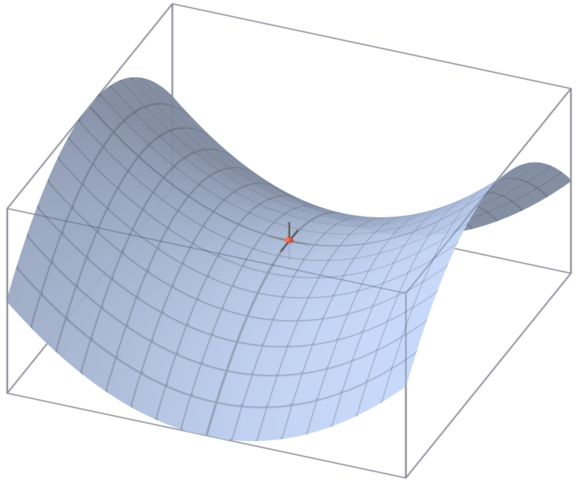
\includegraphics[width=0.7\textwidth]{saddle-point.png}
  \caption{Un punto di sella}
  \label{fig:04-sella}
\end{figure}
%%%%%%%%%%%%%%%%%%%%%%%%%%%%%%%%%%%%%%%%%%%%%%%%%%%%%%%%%%%%%%%%%%%%%%%%%
Notiamo che anche $g''(x_0)$ rimane indipendente da $\calN$ nel limite $\calN\to\infty$. Per svolgere l'integrale (\ref{eq:04-residui}) ragioniamo in questo modo: tenendo conto che nel limite $\calN\to\infty$ il minimo in direzione $x$ è {\em molto profondo} e il massimo in direzione $y$ è {\em molto piccato}, spezziamo l'integrale circolare in due parti: un breve tratto (da $-\varepsilon$ a $\varepsilon$), che possiamo considerare rettilineo, in direzione immaginaria; e poi il resto della circonferenza:
\be
\label{eq:04-spezza}
\frac{1}{2\pi i}\oint \frac{f^\calN}{z^{\calE+1}}\de z =
\frac{1}{2\pi i}\left\{ \int_{-\varepsilon}^{\varepsilon}\frac{f^\calN}{y^{\calE+1}} i \de y
+\int_{C}\frac{f^\calN}{z^{\calE+1}}\de z\right\}
\ee
in cui la curva $C$ nel secondo integrale a destra è quasi tutta la circonferenza tranne il pezzettino di lunghezza $2\varepsilon$ che abbiamo spostato nell'integrale in $\de y$. Come vedremo in seguito, nel limite $\calN\to\infty$ l'integrale su $C$ nella (\ref{eq:04-spezza}) diventa trascurabile; per il momento lo ignoriamo. Per quel che riguarda invece il primo integrale, considerando che solo la regione immediatamente vicina a $x_0$ dà contributi significativi, siamo liberi di mandare $\varepsilon\to\infty$. Se approssimiamo $g(z)$, in direzione $y$, con il suo sviluppo in serie di Taylor al secondo ordine,
\be
g(z) \simeq g(x_0) - \frac{1}{2}y^2g''(x_0)\quad\mbox{\textrm{in direzione}}\ y
\ee
otteniamo immediatamente
\be
\label{eq:04-gammanu}
\Gamma(\calN,U) \simeq \frac{1}{2\pi}\frac{f^\calN(x_0)}{x_0^{\calE+1}}\int_{-\infty}^{\infty}\de y\; e^{-\calN a y^2/2} = \frac{f^\calN(x_0)}{x_0^{\calE+1}\sqrt{2\pi\calN a}}
\ee
in cui abbiamo posto $g''(x_0)\equiv a$. Possiamo quindi scrivere
\be
\frac{1}{\calN}\ln\Gamma(\calN,U) = \ln f(x_0) - \frac{\calE+1}{\calN}\ln x_0 - \frac{1}{2\calN}\ln(2\pi\calN a)
\ee
Notiamo due cose: prima di tutto possiamo porre $(\calE+1)/\calN\simeq U$, perché $\calE\gg 1$; in secondo luogo vediamo che l'ultimo termine scompare nel limite $\calN\to\infty$ in virtù del fatto che $a$ è indipendente da $\calN$. Otteniamo quindi
\be
\label{eq:04-lgamma}
\frac{1}{\calN}\ln\Gamma(\calN,U) = \ln\left(\sum_k w_k e^{-\beta E_k}\right) + \beta U
\ee
Finalmente possiamo scrivere
\bea
\frac{\aspetta{n_r}}{\calN} &=& w_r \frac{1}{\calN}\dpar{\ln\Gamma}{w_r}\Big|_{w_r = 1\;\;\forall\;\;r}\nonumber\\
&=& \left[ \frac{w_r e^{-\beta E_r}}{\sum_k w_k e^{-\beta E_K}} + w_r\dpar{\beta}{w_r}
\left(U - \frac{\sum_k w_k E_k e^{-\beta E_k}}{\sum_k w_k e^{-\beta E_k}} \right)  \right]_{w_r = 1\;\;\forall\;\;r}
\eea
L'ultima parentesi tonda nella precedente è identicamente nulla, e otteniamo
\be
\frac{\aspetta{n_r}}{\calN} = \frac{e^{-\beta E_r}}{\sum_k e^{-\beta E_k}}
\ee
Alla fine di questo lungo viaggio abbiamo scoperto che il valor medio $\aspetta{n_r}$ coincide col valore più probabile $n_r^*$. Ci restano due cose da fare; la prima è dimostrare che l'integrale su $C$, nell'eq. (\ref{eq:04-spezza}), è trascurabile; la seconda è mostrare che le fluttuazioni di $\aspetta{n_r}$ sono ininfluenti e scompaiono nel limite termodinamico. Se non lo fossero l'uguaglianza $n_r^* = \aspetta{n_r}$ potrebbe essere una mera coincidenza numerica, derivante da una distribuzione molto larga. Scopriremo invece che la distribuzione dei set $\nkset$, nel limite $\calN\to\infty$, è talmente piccata intorno al valore più probabile che a tutti gli effetti pratici possiamo considerare $n_r^*$ al posto di $\aspetta{n_r}$.

Iniziamo dal primo problema, l'ininfluenza del secondo integrale nel membro a destra della (\ref{eq:04-spezza}). Dobbiamo dimostrare che nel limite $\calN\to\infty$ l'integrale
\be
\frac{1}{2\pi i}\int_C\frac{f^\calN(z)}{z^{\calE+1}}\de z
\ee
dà un contributo trascurabile. Sappiamo già che $f(z)$ ha, in $x_0$, un minimo molto profondo in direzione reale e un massimo estremamente piccato in direzione immaginaria. Assumiamo ora (ipotesi che andrà verificata in seguito) che per ogni valore di $z$ sulla curva $C$ valga
\be
|f(z)| \le M\quad M < f(x_0)
\ee
Avremo quindi
\be
\frac{1}{2\pi i}\int_C\frac{f^\calN(z)}{z^{\calE+1}}\de z \le
\frac{1}{2\pi}\frac{M^\calN}{x_0^{\calE+1}} \oint\de\theta \simeq
\left(\frac{M}{x_0^U}\right)^\calN = \left(\frac{f(x_0)}{x_0^U}\right)^\calN\left(\frac{M}{f(x_0)}\right)^\calN
\ee
Confrontando il risultato appena ottenuto con la (\ref{eq:04-gammanu}) si vede subito che il secondo integrale nella (\ref{eq:04-spezza}) dà un contributo trascurabile. Ma ciò è vero solo se $M = f(x_0)$ solo per $z = x_0$. Immaginiamo che per un certo angolo $\phi$ tutti i termini della serie che definisce $f(z)$ divengano reali (questo è il disastro che vogliamo evitare). Ciò implicherebbe che tutte le quantità $E_k\phi$ sono multiple intere di $2\pi$:
\be
E_k = m_k\frac{2\pi}{\phi}
\ee
Ricordando che le $E_k$ sono numeri interi, per $2\pi/\phi > 1$ avremmo $2\pi/\phi = p/q$, con $p, q$ interi e $p > 1$. Ciò implicherebbe che $p$ è un divisore comune a tutte le $E_k$, cosa che abbiamo già escluso. Dunque il disastroso angolo $\phi$ non esiste e il secondo integrale dà effettivamente un contributo trascurabile nel limite $\calN\to\infty$.

Resta da verificare che le fluttuazioni non distruggono la nostra costruzione. Dobbiamo dunque trovare il valore di
\be
\aspetta{(\Delta n_r)^2} = \aspetta{[n_r - \aspetta{n_r}]^2} = \aspetta{n_r^2} - \aspetta{n_r}^2
\ee
Proviamo a calcolare (tenendo sempre conto della regola per cui alla fine del calcolo tutte le $w_r$ sono poste uguali a $1$)
\bea
\left( w_r\dpar{}{w_r} \right)\left( w_r\dpar{}{w_r} \right)\ln\Gamma &=&
\left( w_r\dpar{}{w_r} \right) w_r \left[ \frac{1}{\Gamma}\dpar{\Gamma}{w_r} \right] \nonumber \\
&=& w_r\left\{ \frac{\Gamma'}{\Gamma} + w_r\frac{\Gamma''}{\Gamma} \right\} - w_r^2\left( \frac{\Gamma'}{\Gamma} \right)^2
\eea
L'apice su $\Gamma$ indica derivazione rispetto a $w_r$. Nell'ultimo termine riconosciamo immediatamente $\aspetta{n_r}^2$. Per i primi due è necessario un minimo di lavoro, ma si vede facilmente che la loro somma è proprio uguale a
\be
\aspetta{n_r^2} = \frac{1}{\Gamma}\left( w_r\dpar{}{w_r} \right)\left( w_r\dpar{}{w_r} \right)\Gamma
\ee
Tenendo conto della (\ref{eq:04-lgamma}) scriviamo
\be
\frac{\aspetta{(\Delta n_r)^2}}{\calN} = w_r\dpar{}{w_r}\left\{ \frac{w_r e^{-\beta E_r}}{\sum_k w_k e^{-\beta E_k}}
+\dpar{\beta}{w_r}\left[ U - \frac{\sum_k w_k E_k e^{-\beta E_k}}{\sum_k w_k e^{-\beta E_k}}
\right]\right\}
\ee
Il termine tra parentesi quadre nella precedente è identicamente nullo, ma ci resta ancora una derivata da fare:
\be
\frac{\aspetta{(\Delta n_r)^2}}{\calN} = \frac{w_r e^{-\beta E_r}}{\sum_k w_k e^{-\beta E_k}}
- \left( \frac{w_r e^{-\beta E_r}}{\sum_k w_k e^{-\beta E_k}} \right)^2
+ w_r\left( \dpar{\beta}{w_r} \right)\dpar{}{\beta}\left\{ \frac{w_r e^{-\beta E_r}}{\sum_k w_k e^{-\beta E_k}} \right\}
\ee
Riconosciamo immediatamente i primi due termini, e tralasciando per un istante la derivata di $\beta$ rispetto a $w_r$ otteniamo
\be
\label{eq:04-terzu}
\frac{\aspetta{(\Delta n_r)^2}}{\calN} = \frac{\aspetta{n_r}}{\calN} - \left( \frac{\aspetta{n_r}}{\calN} \right)^2
+ w_r \dpar{\beta}{w_r} \frac{\aspetta{n_r}}{\calN} (U - E_r)
\ee
La dipendenza di $\beta$ da $w_r$ (che pure alla fine del conto sono poste tutte a $1$) deriva dal fatto che $\beta$ è definito tramite l'equazione
\be
U = \frac{\sum_k w_k E_k e^{-\beta E_k}}{\sum_k w_k e^{-\beta E_k}}
\ee
con la richiesta $U = \mathrm{costante}$. Utilizziamo quest'ultima relazione per scrivere
\be
\label{eq:04-dlnu}
\de\ln U = 0
\ee
Per semplificare la notazione introduciamo le quantità
\be
s_n = \sum_r w_r E_r^n e^{-\beta E_r}
\ee
e scriviamo dunque $\ln U = \ln s_1 - \ln s_0$. Quindi, per la (\ref{eq:04-dlnu}), variando $\beta$ e solo una delle $w_k$, diciamo $w_r$, abbiamo
\be
\frac{\de s_1}{s_1} - \frac{\de s_0}{s_0} =
\frac{E_r e^{-\beta E_r}\de w_r - s_2\de\beta}{s_1} - \frac{e^{-\beta E_r}\de w_r - s_1\de\beta}{s_0} = 0
\ee
Possiamo quindi scrivere
\be
w_r\dpar{\beta}{w_r} = \frac{w_r e^{-\beta E_r}}{s_0} \frac{E_r - (s_1/s_0)}{(s2/s_0) - (s_1/s_0)^2}
\ee
e ripristinando la solita notazione otteniamo finalmente
\be
w_r\dpar{\beta}{w_r} = \frac{\aspetta{n_r}}{\calN} \frac{E_r - U}{\aspetta{E_r^2} - U^2}
\ee
Inserendo l'ultima equazione nella (\ref{eq:04-terzu}) possiamo scrivere
\be
\frac{\aspetta{(\Delta n_r)^2}}{\calN} = \frac{\aspetta{n_r}}{\calN}
\left\{
1 - \frac{\aspetta{n_r}}{\calN} \left[ 1 + \frac{(E_r-U)^2}{\aspetta{(E_r-U)^2}} \right]
\right\}
\ee
e per la fluttuazione relativa troviamo
\be
\frac{\aspetta{(\Delta n_r)^2}}{\aspetta{n_r}^2} = \frac{1}{\aspetta{n_r}} - \frac{1}{\calN}
\left\{
1 + \frac{(E_r-U)^2}{\aspetta{(E_r-U)^2}}
\right\}
\ee
Se vogliamo che $P_r$ abbia un limite finito, nel limite $\calN\to\infty$ anche $\aspetta{n_r}\to\infty$: quindi le fluttuazioni sono infinitamente soppresse, la distribuzione delle $n_r$ si avvicina a una delta di Dirac e il valore più probabile coincide con il valore medio.

%%%%%%%%%%%%%%%%%%%%%%%%%%%%%%%%%%%%%%%%%%%%%%%%%%%%%%%%%%%%%%%%%%%%%%%%
\section{Significato fisico delle quantità statistiche}
\label{sec:04-significato}
%%%%%%%%%%%%%%%%%%%%%%%%%%%%%%%%%%%%%%%%%%%%%%%%%%%%%%%%%%%%%%%%%%%%%%%%

Riprendiamo l'espressione per la distribuzione canonica:
\be
\label{eq:04-distcan}
P_r \equiv \frac{\aspetta{n_r}}{\calN} = \frac{e^{-\beta E_r}}{\sum_s e^{-\beta E_s}}
\ee
in cui $\beta$ è determinato dall'equazione
\be
\label{eq:04-defbeta}
U = \frac{\sum_r E_r e^{-\beta E_r}}{\sum_r e^{-\beta E_r}} = -\dpar{}{\beta}\ln\left\{ \sum_r e^{-\beta E_r} \right\}
\ee
Per ricavare informazioni sulle varie quantità fisiche del sistema macroscopico ricordiamo alcune relazioni termodinamiche fondamentali che riguardano l'energia libera di Helmholtz $A = U - TS$:
\be
\label{eq:04-dA}
\de A = \de U - T\de S - S\de T = -S\de T - P\de V + \mu\de N
\ee
\be
\label{eq:04-maxdA}
S   = -\dparc{A}{T}{N,V} \quad
P   = -\dparc{A}{V}{N,T} \quad
\mu =  \dparc{A}{N}{V,T}
\ee
e infine
\be
\label{eq:04-defU}
U = A + TS = A - T\dparc{A}{T}{N,V} = -T^2\left[ \dpar{}{T} \left( \frac{A}{T} \right) \right]_{N,V}
= \left[ \dpar{(A/T)}{(1/T)} \right]_{N,V}
\ee
Confrontando la (\ref{eq:04-defU}) con la (\ref{eq:04-defbeta}) ci accorgiamo subito che possiamo stabilire una corrispondenza tra quantità fisiche macroscopiche e le quantità statistiche. In particolare troviamo (come si poteva facilmente immaginare) che
\be
\beta = \frac{1}{kT}
\ee
ma soprattutto
\be
A = -kT \ln\left\{ \sum_r e^{-\beta E_r} \right\}
\ee
che riscriviamo in questo modo:
\be
\label{eq:04-introQ}
A = -kT \ln Q_N(V,T)
\ee
in cui $Q_N(V,T) = \sum_r e^{-\beta E_r}$ è la così detta {\em funzione di partizione canonica} del sistema. La dipendenza di $Q$ da $N$ e $T$ è abbastanza ovvia. La dipendenza da $V$ è data dalla dipendenza diretta dai livelli di energia $E_r$.

Nota la funzione di partizione $Q$ di un sistema, e dunque l'energia libera di Helmholtz $A$, possono essere ricavate tutte le altre quantità termodinamiche. Per entropia, pressione e potenziale chimico abbiamo già visto: equazione (\ref{eq:04-maxdA}). Per il calore specifico a volume costante abbiamo
\be
\label{eq:04-cvA}
C_V = \dparc{U}{T}{N,V} = -T\left( \frac{\partial^2 A}{\partial T^2} \right)_{N,V}
\ee
Occorre tenere presente che l'energia libera $A(N,V,T)$ è una quantità estensiva: ciò implica che dev'essere una funzione omogenea di grado $1$ rispetto a $N$ e $V$, a loro volta estensive. Il fatto che sia omogenea di grado $1$ significa che
\be
A(\alpha N, \alpha V, T) = \alpha A(N,V,T)
\ee
Ricordiamo ora il teorema di Eulero sulle funzioni omogenee: se $f(x_1,\dots x_n)$ è una funzione omogenea di grado $k$, allora deve valere la relazione
\be
\sum_i\dpar{f}{x_i}x_i = kf(x_1,\dots x_n)
\ee
La dimostrazione è abbastanza semplice: definiamo $x_i' = \alpha x_i$. Per definizione di funzione omogenea di grado $k$ otteniamo
\be
f(x_1',\dots x_n') = \alpha^k f(x_1,\dots x_n)
\ee
Derivando rispetto a $\alpha$ entrambi i membri e usando la {\em chain rule} otteniamo
\be
\sum_i\dpar{f}{x_i'}\dpar{x_i'}{\alpha} = k\alpha^{k-1} f(x_1,\dots x_n)
\ee
ma
\be
\dpar{x_i'}{\alpha} = x_i
\ee
e scegliendo $\alpha = 1$ otteniamo la dimostrazione. Questo teorema ci permette di scrivere
\be
\label{eq:04-eulerA}
N\dparc{A}{N}{V,T} + V\dparc{A}{V}{N,T} = A
\ee
Per l'energia libera di Gibbs otteniamo
\be
G = A + PV = A - V\dparc{A}{V}{N,T} = N\dparc{A}{N}{V,T} = N\mu
\ee
in cui nel penultimo passaggio abbiamo usato la (\ref{eq:04-eulerA}).

Per l'entropia, poiché $P_r = \exp(-\beta E_r)/Q$, troviamo
\be
\aspetta{\ln P_r} = -\ln Q -\beta\aspetta{E_r} = \beta(A - U) = -S/k
\ee
e dunque
\be
\label{eq:04-sprob}
S = -k\aspetta{\ln P_r} = -k \sum_r P_r\ln P_r
\ee
Questa è una relazione estremamente interessante perché dimostra che l'entropia di un sistema fisico è determinata completamente e unicamente dai valori $P_r$ della probabilità che il sistema ha di essere in un determinato stato accessibile. Questo fatto ha un'importanza che è difficile sottovalutare, e porta a diverse conclusioni notevoli. Per esempio, se lo stato di minima energia ({\em ground state}) di un sistema è non degenere, a temperatura nulla il sistema non avrà alternative e potrà stare in un unico stato, col risultato che solo una delle $P_r$ vale $1$, e tutte le altre $0$. Otteniamo dunque un'entropia nulla. Questo è il teorema di Nernst, o terzo principio della termodinamica.

Si può notare che la (\ref{eq:04-sprob}) vale anche nel microcanonico: poiché in quel caso ogni microstato è equiprobabile e il numero dei microstati è $\Omega$, abbiamo che $P_r = 1/\Omega$ per ogni $r$. Quindi
\be
S = -k\sum_{r=1}^\Omega\left\{ \frac{1}{\Omega}\ln\left( \frac{1}{\Omega} \right) \right\} = k\ln\Omega
\ee

%%%%%%%%%%%%%%%%%%%%%%%%%%%%%%%%%%%%%%%%%%%%%%%%%%%%%%%%%%%%%%%%%%%%%%%%
\section{Espressioni alternative per la funzione di partizione}
\label{sec:04-espressioni-alternative}
%%%%%%%%%%%%%%%%%%%%%%%%%%%%%%%%%%%%%%%%%%%%%%%%%%%%%%%%%%%%%%%%%%%%%%%%

In tutto ciò che precede bisogna fare attenzione a non confondere gli stati $r$ con energia $E_r$, in cui il sistema fisico può stare, con i possibili livelli di energia del sistema. In altre parole abbiamo definito la funzione di partizione proprio come la somma su tutti gli stati in cui il sistema può trovarsi, e non come una somma sui livelli di energia. Per un sistema con spettro discreto, il livello $i$ sarà o potrà essere degenere; sia dunque $g_i$ il numero di stati che ammettono energia $E_i$. La formula per la funzione di partizione diventa
\be
Q_N(V,T) = \sum_i g_i e^{-\beta E_i}
\ee
e corrispondentemente la probabilità $P_i$ che il sistema sia in uno stato con energia $E_i$ diventa
\be
P_i = \frac{g_i e^{-\beta E_i}}{\sum_k g_k e^{-\beta E_k}}
\ee
Questo perché, chiaramente, tutti gli stati con uguale energia $E_i$ hanno le stesse probabilità di essere raggiunti.
L'introduzione del fattore di molteplicità risulta importante quando consideriamo sistemi classici in cui lo spettro di energia è continuo. Bisogna allora chiedersi quale sia la probabilità $P(E)\,\de E$ di trovare il sistema in uno stato con energia compresa tra $E$ e $E + \de E$. Ovviamente questa probabilità sarà data dal prodotto del peso di Boltzmann $e^{-\beta E}$ per il ``numero'' di livelli contenuti nell'intervallino energetico in considerazione. Scriviamo dunque
\be
P(E)\,\de E \propto g(E)e^{-\beta E}\de E
\ee
in cui $g(E)$ è la densità degli stati intorno al valore di energia $E$. Normalizzando otteniamo
\be
P(E)\,\de E = \frac{g(E)e^{-\beta E}\de E}{\int_0^\infty g(E)e^{-\beta E}\de E}
\ee
Il denominatore dell'equazione precedente è un'espressione alternativa della funzione di partizione del sistema:
\be
\label{eq:04-laplace}
Q_N(V,T) = \int_0^\infty g(E)e^{-\beta E}\de E
\ee
Per il valore di osservazione di un generico osservabile $f$ otteniamo
\be
\aspetta{f\,} = \frac{\int_0^\infty f(E)g(E)e^{-\beta E}\de E}{\int_0^\infty g(E)e^{-\beta E}\de E}
\ee
Notiamo una cosa interessante: osservando la (\ref{eq:04-laplace}) e poiché $\beta > 0$, vediamo che la funzione di partizione $Q(\beta)$ è la trasformata di Laplace della densità degli stati $g(E)$. Possiamo dunque ottenere $g(E)$, nota la funzione di partizione, come la trasformata di Laplace inversa di $Q(\beta)$:
\bea
\label{eq:04-gfromq}
g(E) &=& \frac{1}{2\pi i}\int_{\beta'-i\infty}^{\beta'+i\infty} e^{\beta E}Q(\beta)\de\beta\quad(\beta' > 0)
\nonumber \\
&=& \frac{1}{2\pi}\int_{-\infty}^{\infty}e^{(\beta'+i\beta'')E}Q(\beta'+i\beta'')\de\beta''
\eea
in cui adesso $\beta = \beta' + i\beta''$ è trattato come una variabile complessa. Il cammino d'integrazione corre parallelo all'asse immaginario e può essere deformato se necessario.

%%%%%%%%%%%%%%%%%%%%%%%%%%%%%%%%%%%%%%%%%%%%%%%%%%%%%%%%%%%%%%%%%%%%%%%%
\section{Il gas ideale classico}
\label{sec:04-gas-ideale}
%%%%%%%%%%%%%%%%%%%%%%%%%%%%%%%%%%%%%%%%%%%%%%%%%%%%%%%%%%%%%%%%%%%%%%%%

Consideriamo ora sistemi classici che ammettono una descrizione in termini di spazio delle fasi. Il sistema tipico che abbiamo in mente è il gas ideale classico, che vedremo in dettaglio tra poco. Sia $\dephi \equiv \de^{3N}q\de^{3N}p$ un volumetto elementare nello spazio delle fasi. Dovrebbe risultare chiaro che l'espressione per $P_r$ che abbiamo ricavato nelle sezioni precedenti ci permette di scrivere
\be
\rho(q,p) \propto \exp[-\beta\Ham(q,p)]
\ee
Infatti la densità $\rho$ dei punti rappresentativi nello spazio delle fasi è una misura della probabilità di trovare un punto rappresentativo nelle vicinanze della posizione $(q,p)$, e questa probabilità dipende dall'energia, ovvero dall'hamiltoniana del sistema. Il valore d'osservazione di un generico osservabile $f$ diventa quindi
\be
\aspetta{f} = \frac{\int f(q,p) e^{-\beta\Ham(q,p)}\dephi}{\int e^{-\beta\Ham(q,p)}\dephi}
\ee
Il denominatore di questa espressione è direttamente correlato con la funzione di partizione del sistema, ma per scrivere realmente la funzione di partizione dobbiamo ricordarci della correzione di Gibbs e del fattore $h$ elevato al giusto numero di gradi di liberta: quindi
\be
Q_N(V,T) = \frac{1}{N!h^{3N}}\int e^{-\beta\Ham(q,p)}\dephi
\ee
\`E chiaro che questi ultimi integrali vanno calcolati sull'intero spazio delle fasi.

Consideriamo ora il gas ideale. L'energia è puramente cinetica (nessuna interazione tra gli atomi):
\be
\Ham(q,p) = \sum_{i=1}^{N}\frac{p_i^2}{2m}
\ee
in cui $m$ è la massa delle particelle. Calcolando la funzione di partizione ci accorgiamo subito che l'integrazione sulle coordinate dà solo un fattore $V^N$ (come d'altronde abbiamo già visto nei capitoli precedenti); possiamo dunque scrivere
\be
Q_N(V,T) = \frac{V^N}{N!h^{3N}}\int e^{-(\beta/2m)\sum_i p_i^2}\prod_{i=1}^{N}\de^3 p_i
\ee
Gli integrali sulle $p_i$ in nulla differiscono l'uno dall'altro; otteniamo così
\be
Q_N(V,T) = \frac{V^N}{N!h^{3N}}\left[ \int_0^\infty e^{-p^2/2mkT} (4\pi p^2 \de p)\right]^{N}
\ee
L'integrale può essere calcolato facilmente grazie a un utile trucco. Consideriamo infatti l'integrale gaussiano
\be
I_0(\alpha) = \int_{-\infty}^{\infty}\de x e^{-\alpha x^2} = \sqrt{\pi/\alpha}
\ee
Consideriamo ora
\be
I_2(\alpha) = \int_{-\infty}^{\infty}\de x x^2 e^{-\alpha x^2} = -\dtot{I_0(\alpha)}{\alpha} = \frac{1}{2}\sqrt{\pi/\alpha^3}
\ee
Ora, poiché la nostra funzione integranda è pari, possiamo moltiplicare per $1/2$ ed estendere l'integrale da $-\infty$ a $\infty$. Inoltre nel nostro caso $\alpha = 1/2mkT$. Otteniamo subito
\be
Q_N(V,T) = \frac{1}{N!}\left[ V \left(\frac{2\pi mkT}{h^2}\right)^{3/2} \right]^{N}
\ee
I più volenterosi potrebbero notare che la quantità
\be
\lambda \equiv \frac{h}{\sqrt{2\pi mkT}}
\ee
ha le dimensioni di una lunghezza, in modo tale da rendere la funzione di partizione adimensionale. La quantità $\lambda$ è la lunghezza d'onda termica, o lunghezza d'onda di de Broglie, e la vedremo spesso nel seguito. Quindi in forma compatta
\be
Q_N(V,T) = \frac{1}{N!}(V/\lambda^3)^N
\ee
Per l'energia libera di Helmholtz otteniamo
\be
A(N,V,T) = -kT\ln Q_N(V,T) = NkT\left[ \ln\left\{ \frac{N}{V}\left( \frac{h^2}{2\pi mkT} \right)^{3/2} \right\} - 1 \right]
\ee
La stessa espressione era stata ricavata nel Capitolo \ref{cap:basi}, con un procedimento ben più tortuoso. Tutte le altre grandezze fisiche o relazioni fondamentali (potenziale chimico, entropia, equazione di stato) hanno le stesse espressioni che abbiamo già incontrato, quindi inutile starle a ripetere.

Dobbiamo però notare una cosa importante; considerando la funzione di partizione per una singola particella, otteniamo immediatamente
\be
Q_1(V,T) = V / \lambda^3
\ee
e dunque possiamo scrivere
\be
Q_N(V,T) = \frac{1}{N!}[Q_1(V,T)]^N
\ee
Questo è un risultato di carattere generale, che non vale solo per il gas ideale classico, ma per tutti i sistemi classici nei quali i costituenti elementari sono supposti non interagire tra loro (in ambito quantistico, come vedremo, le cose cambiano notevolmente).

Proviamo ora a calcolare la funzione di partizione del gas ideale classico partendo dalla densità degli stati. Calcoliamo prima di tutto $Q_1(\beta)$ (nel seguito omettiamo la dipendenza dal volume):
\be
\label{eq:04-q1eps}
Q_1(\beta) = \int_0^\infty\de\varepsilon \densa e^{-\beta\varepsilon}
\ee
in cui abbiamo indicato con $\densa$ la densità degli stati di singola particella. Per calcolarla ragioniamo come segue. Sia $\Sigma(P)$ il numero di microstati per una particella racchiusa in un volume $V$ e con momento (in modulo) minore di $P$. Abbiamo
\be
\Sigma(P) = \frac{1}{h^3}\int\de^3 q\int\de^3 p = \frac{4\pi V}{h^3}\int_0^P p^2\de p = \frac{4\pi V P^3}{3h^3}
\ee
Per trovare il numero di microstati con momento compreso nell'intervallo $(p, p+\de p)$ calcoliamo
\be
g(p)\de p = \dtot{\Sigma(p)}{p}\de p = \frac{4\pi V}{h^3}p^2\de p
\ee
Se ora usiamo il fatto che $\varepsilon = p^2/2m$ otteniamo subito
\be
\densa =\frac{2\pi V}{h^2}(2m)^{3/2}\varepsilon^{1/2}\de\varepsilon
\ee
L'integrale (\ref{eq:04-q1eps}) può essere svolto facilmente con il cambio di variabile $x^2\equiv\varepsilon$, e il risultato è, senza nessuna sorpresa
\be
Q_1(\beta) = V / \lambda^3
\ee

Come ultimo punto di questa sezione ci proponiamo di calcolare la densità degli stati $g(E)$ per l'intero sistema come antitrasformata di Laplace della funzione di partizione. Abbiamo, applicando la (\ref{eq:04-gfromq}),
\be
g(E) = \frac{V^N}{N!}\left( \frac{2\pi m}{h^2} \right)^{3N/2}\frac{1}{2\pi i}\int_{\beta'-i\infty}^{\beta'+i\infty}
\frac{e^{\beta E}}{\beta^{3N/2}}\de\beta\quad(\beta' > 0)
\ee
Considerando che l'unico polo della funzione è in $\beta=0$ (un polo di ordine $3N/2$), l'esponenziale al denominatore ci suggerisce di chiudere il cammino di integrazione all'infinito andando verso $\beta\to -\infty$. Dobbiamo sostanzialmente saper svolgere l'integrale
\be
\frac{1}{2\pi i}\oint \de z \frac{e^{z\beta}}{z^{n}}
\ee
in cui il circuito chiuso circonda il punto $z=0$. Se una funzione $f(z)$ presenta un polo di ordine $n$ nel punto $z_0$, il teorema dei residui ci dice che il residuo in quel punto sarà dato da
\be
R = \frac{1}{(n-1)!}\lim_{z\to z_0}\left\{\frac{\de^{n-1}}{\de z^{n-1}}\left[(z-z_0)^n f(z)\right]\right\}_{z=z_0}
\ee
Nel nostro caso abbiamo un polo in $z=0$, con $n = 3N/2$ e $f(z) = e^{zE}/z^n$. Quindi
\be
R = \frac{1}{(n-1)!}\lim_{z\to 0}\left\{\frac{\de^{n-1}}{\de z^{n-1}}\left[e^{zE}\right]\right\}_{z=0}
= \frac{E^{n-1}}{(n-1)!}
\ee
Otteniamo dunque
\be
g(E) = \frac{V^N}{N!}\left(\frac{2\pi m}{h^2}\right)^{3N/2}\frac{E^{3N/2-1}}{(3N/2-1)!}
\ee
che è (per fortuna) il risultato corretto che avevamo già trovato, a patto di confondere $3N/2-1 \simeq 3N/2$, cosa che nel limite termodinamico è perfettamente lecita.

%%%%%%%%%%%%%%%%%%%%%%%%%%%%%%%%%%%%%%%%%%%%%%%%%%%%%%%%%%%%%%%%%%%%%%%%
\section{Fluttuazioni dell'energia}
\label{sec:04-fluttuazioni}
%%%%%%%%%%%%%%%%%%%%%%%%%%%%%%%%%%%%%%%%%%%%%%%%%%%%%%%%%%%%%%%%%%%%%%%%

Nella sezione precedente abbiamo visto, considerando il gas ideale classico, che con il formalismo canonico riusciamo a ottenere, nel limite termodinamico, gli stessi risultati fisici che avevamo ottenuto con il formalismo microcanonico. Questo è un risultato generale che non si applica solo al gas ideale classico. D'altronde il contrario avrebbe significato una catastrofe: se due formalismi diversi che dovrebbero entrambi condurre alla termodinamica ci portano a soluzioni diverse c'è da dubitare di tutti i nostri risultati.

Ci chiediamo però come sia possibile che il miracolo si compia, visto che nel microcanonico l'energia interna del sistema è fissata (o comunque può variare in un piccolo intervallo) mentre nel canonico può, in linea di principio, fluttuare da 0 a infinito.

Prendiamo in considerazione l'energia interna del sistema:
\be
U \equiv \aspetta{E} = \frac{\sum_k E_k e^{-\beta E_k}}{\sum_k e^{-\beta E_k}}
\ee
e proviamo a calcolare la quantità
\be
-\dpar{U}{\beta} = \frac{\sum_k E_k^2 e^{-\beta E_k}}{\sum_k e^{-\beta E_k}}
    - \frac{(\sum_k E_k e^{-\beta E_k})^2}{(\sum_k e^{-\beta E_k})^2}
    = \aspetta{E^2} - \aspetta{E}^2 = \aspetta{(\Delta E)^2}
\ee
in cui la derivata rispetto a $\beta$ è fatta lasciando invariati i livelli di energia $E_k$. Vediamo dunque che la quantità appena calcolata ci fornisce la fluttuazione quadratica media dell'energia interna. Osserviamo ora che
\be
-\dpar{U}{\beta} = kT^2\dpar{U}{T}
\ee
ma tenere tutte le $E_k$ costanti nel processo di derivazione equivale a tenere costante il volume in cui il sistema è racchiuso. Otteniamo dunque, per la fluttuazione relativa dell'energia
\be
\frac{\sqrt{\aspetta{(\Delta E)^2}}}{U} = \frac{\sqrt{kT^2C_V}}{U}
\ee
Notiamo che sia $C_V$ sia $U$ sono quantità estensive, e cioè crescono linearmente con $N$. Nel limite termodinamico otteniamo dunque
\be
\frac{\sqrt{\aspetta{(\Delta E)^2}}}{U} \propto \frac{1}{\sqrt{N}}
\ee
ossia che le fluttuazioni relative scompaiono. In altre parole il valore della densità di energia, anche se in principio può fluttuare, rimane inchiodato al suo valore medio $U/N$ (oppure $U/V$, a seconda dei gusti, visto che in ogni caso $V$, nel limite termodinamico, cresce proporzionalmente a $N$). Questo risultato spiega perché i due \ensembles\ portano agli stessi risultati (nel limite termodinamico!).

Per comprendere meglio la questione chiediamoci in quale maniera l'energia è distribuita tra i vari livelli di energia nell'\ensemble\ canonico, assumendo che l'energia sia una variabile continua. Abbiamo già ottenuto, per la probabilità $P(E)\de E$ che un certo stato abbia energia nell'intervallo $(E,E+\de E)$, il risultato
\be
P(E) \de E \propto g(E) \exp(-\beta E)\de E
\ee
Dunque la densità di probabilità $P(E)$ è il prodotto di due fattori: la densità degli stati, che è una funzione monotonicamente crescente di $E$, e il peso di Boltzmann, che è una funzione monotonicamente decrescente di $E$. L'esponenziale fa sì che $P(E)\to 0$ quando $E\to\infty$, mentre la densità degli stati fa ottiene lo stesso risultato (se si pensa al gas ideale classico come esempio) nel limite $E\to\ 0$. Entrambe le funzioni sono positive; il loro prodotto presenterà dunque un estremo per un certo valore di $E$, diciamo $E^*$. In realtà questo estremo, come vedremo presto, è un massimo. Il valore $E^*$ per il quale c'è il massimo rappresenterà il valore più probabile dell'energia. La condizione per trovare $E^*$ è chiaramente
\be
\frac{\de P(E)}{\de E}|_{E=E^*} = \left[e^{-\beta E}\frac{\de g(E)}{\de E} - \beta g(E)e^{-\beta E}\right]_{E=E^*} = 0
\ee
che possiamo chiaramente riscrivere nel modo seguente:
\be
\frac{\de \ln g(E)}{\de E}|_{E=E^*} = \beta
\ee
Ricordiamo però che il logaritmo della densità degli stati canonica $g(E)$ è, a meno di un fattore $k$, l'entropia microcanonica di un sistema con energia fissata $E$, e ricordando la relazione
\be
\dparc{S(E)}{E}{E=U} = \frac{1}{T}
\ee
otteniamo che all'equilibrio deve valere
\be
E^* = U
\ee
ossia il valore più probabile dell'energia coincide col valor medio. Questo risultato, strettamente parlando, vale solo nel limite termodinamico.

Per analizzare la situazione ancora più a fondo, espandiamo il logaritmo della densità di probabilità $P(E)$ intorno al valore $E^* \simeq U$:
\bea
\ln[e^{-\beta E}g(E)] &=& (-\beta U + S/k) \nonumber \\
&+& \frac{1}{2}\frac{\partial^2}{\partial E^2}\left[\ln\{e^{-\beta E}g(E)\}\right]_{E=U} (E-U)^2 + \cdots \nonumber \\
   &=& -\beta(U-TS) - \frac{(E-U)^2}{2kT^2C_V} + \cdots
\eea
Nel primo passaggio abbiamo sfruttato il fatto che la derivata prima si annulla in virtù della condizione di equilibrio, mentre nel secondo abbiamo usato i passaggi
\be
\left( \frac{\partial^2 S(E)}{\partial E^2} \right)_{E=U} = \left( \frac{\partial}{\partial E}\frac{1}{T} \right)_{E=U}
= - \left( \frac{1}{T^2}\frac{\partial T}{\partial E} \right)_{E=U} = -\frac{1}{T^2 C_V}
\ee
Alla fine otteniamo che nel limite termodinamico la densità di probabilità $P(E)$ è ottimamente approssimata da una gaussiana:
\be
P(E) \propto e^{-\beta(U-TS)}\exp\left( \frac{(E-U)^2}{2kT^2 C_V} \right)
\ee
Va notato che la dispersione della gaussiana coincide col risultato che abbiamo trovato prima per $\aspetta{(\Delta E)^2}$. \`E consolante vedere che mescolando il formalismo canonico con quello microcanonico si ottengono risultati consistenti.

%%%%%%%%%%%%%%%%%%%%%%%%%%%%%%%%%%%%%%%%%%%%%%%%%%%%%%%%%%%%%%%%%%%%%%%%
\section{Il teorema di equipartizione}
\label{sec:04-equipart}
%%%%%%%%%%%%%%%%%%%%%%%%%%%%%%%%%%%%%%%%%%%%%%%%%%%%%%%%%%%%%%%%%%%%%%%%

Consideriamo il valore d'aspettazione della quantità $x_i(\partial\Ham/\partial x_j)$, nella quale $\Ham(q,p)$ è l'hamiltoniana di un sistema fisico e $x_i$ e $x_j$ sono qualsiasi due delle $6N$ coordinate generalizzate $(q,p)$. Utilizzando il formalismo dell'ensemble canonico otteniamo
\be
\gaspetta{x_i\dpar{\Ham}{x_j}} = \frac{\int x_i\dpar{\Ham}{x_j}e^{-\beta\Ham}\dephi}{\int x_i\dpar{\Ham}{x_j}e^{-\beta\Ham}\dephi}
\ee
Consideriamo solo l'integrale al numeratore: integrando su $x_j$ per parti, otteniamo
\be
\int\left[ -\frac{1}{\beta}x_ie^{-\beta\Ham}\Bigg|_{x_1}^{x_2} + \frac{1}{\beta}\int\de x_j\left( \dpar{x_i}{x_j}\right)e^{-\beta\Ham} \right]\de\varphi_j
\ee
$x_1$ e $x_2$ rappresentano gli estremi di integrazione di $x_j$; $\dephi_j$ significa $\dephi$ a cui è stato tolto $\de x_j$. Il primo termine, quello integrato su $x_j$, è nullo. Ciò è facile da comprendere se $x_j$ è un momento, perché l'esponenziale va sempre a zero per $p\to\pm\infty$. Se $x_j$ è una coordinata basta pensare che i limiti di integrazione sono rappresentati dalle pareti della scatola che contiene il sistema. Una parete viene matematicamente modellizzata come un potenziale che va repentinamente a infinito. Dunque anche in questo caso l'esponenziale ammazza tutto. Nel secondo termine notiamo che $\partial x_i/\partial x_j = \delta_{ij}$, e che $\de x_j\dephi_j = \dephi$. Inserendo il tutto nell'equazione di partenza otteniamo
\be
\gaspetta{x_i\dpar{\Ham}{x_j}} = \delta_{ij} kT
\ee
che è indipendente dalla forma precisa di $\Ham$.

Nel caso in cui $x_i = x_j = p_i$ abbiamo
\be
\gaspetta{p_i\dpar{\Ham}{p_i}} = \aspetta{p_i\dot{q}_i} = kT
\ee
mentre invece nel caso $x_i = x_j = q_i$ troviamo
\be
\gaspetta{q_i\dpar{\Ham}{q_i}} = -\aspetta{q_i\dot{p}_i} = kT
\ee
Sommando su $i$ da $1$ a $3N$ otteniamo
\be
\gaspetta{\sum_i p_i\dot{q}_i} = -\gaspetta{\sum_i q_i\dot{p}_i} = 3NkT
\ee
Ora, in molti problemi fisici rilevanti l'hamiltoniana del sistema è una funzione quadratica delle sue coordinate generalizzate; in questo caso, tramite una trasformazione canonica, possiamo sempre scrivere
\be
\label{eq:04-hamab}
\Ham = \sum_k A_k P_k^2 + \sum_k B_k Q_k^2
\ee
Per un tale sistema abbiamo chiaramente
\be
\sum_k\left( P_k\dpar{\Ham}{P_k} + Q_k\dpar{\Ham}{Q_k} \right) = 2\Ham
\ee
e di conseguenza
\be
\aspetta{\Ham} = \frac{1}{2} MkT
\ee
in cui $M$ è il numero totale dei coefficienti $A$ e $B$ diversi da zero nella (\ref{eq:04-hamab}). Ne concludiamo che ciascun termine armonico nell'hamiltoniana trasformata dà un contributo pari a $\frac{1}{2}kT$ all'energia interna del sistema, e dunque un contributo $\frac{1}{2}k$ al calore specifico $C_V$. Questo risultato è noto come il teorema classico dell'equipartizione dell'energia. L'energia termica si equidistribuisce tra i vari gradi di libertà del sistema.

%%%%%%%%%%%%%%%%%%%%%%%%%%%%%%%%%%%%%%%%%%%%%%%%%%%%%%%%%%%%%%%%%%%%%%%%
\section{Sistema di oscillatori armonici}
\label{sec:04-oscarm}
%%%%%%%%%%%%%%%%%%%%%%%%%%%%%%%%%%%%%%%%%%%%%%%%%%%%%%%%%%%%%%%%%%%%%%%%

Consideriamo un sistema di $N$ oscillatori armonici che consideriamo non interagenti. Questo sistema riveste una particolare importanza, come vedremo nel seguito, e ci fornità la base, per esempio, per studiare sia la radiazione di corpo nero (o la statistica di un gas di fotoni) sia il calore specifico dei solidi (ossia la statistica di un gas di fononi).

Partiamo con la situazione classica. Poiché gli oscillatori sono indipendenti possiamo calcolare la funzione di partizione di singola oscillatore e poi elevare alla $N$ per ottenere la funzione di partizione totale. Anticipiamo subito che ometteremo il fattore correttivo di Gibbs $1/N!$ in quanto immaginiamo che ogni oscillatore vibri intorno a una sua posizione d'equilibrio; gli oscillatori sono per così dire localizzati, e quindi distinguibili. Questo sarà un punto che riprenderemo in esame quando vedremo la statistica dei fotoni.

Per il singolo oscillatore (unidimensionale) di frequenza $\omega$ abbiamo l'hamiltoniana
\be
\Ham = \frac{1}{2m}p^2 + \frac{1}{2}m\omega^2 q^2
\ee
e per la funzione di partizione di singolo oscillatore abbiamo l'espressione
\be
Q_1(\beta) = \int_{-\infty}^{\infty}\int_{-\infty}^{\infty}\frac{\de p\de q}{h}\exp\left( -\beta\left[ \frac{1}{2m}p^2 + \frac{1}{2}m\omega^2 q^2\right] \right)
\ee
Riconosciamo subito tranquilli integrali gaussiani e possiamo immediatamente scrivere
\be
Q_1(\beta) = \frac{1}{h}\left(\frac{2\pi}{\beta m\omega^2}\right)^{1/2}\left(\frac{2\pi m}{\beta}\right)^{1/2}
= \frac{1}{\beta\hbar\omega} = \frac{kT}{\hbar\omega}
\ee
Notiamo incidentalmente che almeno dal punto di vista dimensionale il risultato è corretto: sia $kT$ sia $\hbar\omega$ hanno le dimensioni di un'energia, quindi il loro rapporto è adimensionale. Notiamo anche che il risultato rappresenta il conteggio classico dei microstati accessibili al singolo oscillatore, cioè $kT$ diviso la spaziatura tra i livelli quantistici, cioè $\hbar\omega$. Per la funzione di partizione totale abbiamo
\be
Q_N(\beta) = [Q_1(\beta)]^N = \left(\frac{kT}{\hbar\omega}\right)^N
\ee
e quindi per l'energia libera di Helmoltz
\be
A = -kT\ln Q_N = NkT\ln\left(\frac{\hbar\omega}{kT}\right)
\ee
A questo punto è facile ricavare tutte le quantità fisiche rilevanti:
\bea
\mu &=& \phantom{-}\dparc{A}{N}{V,T} = kT\ln\left(\frac{\hbar\omega}{kT}\right) \\
P   &=& \phantom{-}\dparc{A}{V}{N,T} = 0 \\
S   &=&          - \dparc{A}{T}{N,V} = Nk\left[\ln\left(\frac{kT}{\hbar\omega}\right)+1\right]
\eea
Per l'energia interna $U$ possiamo scegliere di calcolarla in due modi:
\be
U = -\dparc{\ln Q_N}{\beta}{E_r} = A + TS
\ee
ma ovviamente in entrambi i casi il risultato è
\be
U = NkT
\ee
Otteniamo infine
\be
C_P = C_V = Nk
\ee
L'energia media per oscillatore è perfettamente in accordo col teorema di equipartizione, e cioè $2\times \frac{1}{2}kT$, poiché abbiamo due termini quadratici indipendenti per singolo oscillatore.

Nota la funzione di partizione possiamo pensare di determinare la densità degli stati $g(E)$ usando l'equazione (\ref{eq:04-gfromq}):
\be
g(E) = \frac{1}{(\hbar\omega)^N}\frac{1}{2\pi i}\int_{\beta'-i\infty}^{\beta'+i\infty}
\frac{e^{\beta E}}{\beta^N}\de\beta\quad(\beta' > 0)
\ee
Il teorema dei residui (vedi il conto fatto per il gas ideale classico: le cose vanno allo stesso modo) ci permette di trovare subito
\be
g(E) = \frac{1}{(\hbar\omega)^N}\frac{E^{N-1}}{(N-1)!}
\ee
Per verificare la correttezza della precedente potremmo pensare di usarla per calcolare l'entropia. Prendendo $N\gg 1$ e usando la formula di Stirling troviamo
\be
S(N,E) = k\ln g(E) \simeq Nk\left[ \ln\left( \frac{E}{N\hbar\omega} \right) + 1 \right]
\ee
e per la temperatura d'equilibrio microcanonica del sistema troviamo subito
\be
T = \dparc{S}{E}{N}^{-1} = \frac{E}{Nk}
\ee
Eliminando $E$ tra le ultime due equazioni ritroviamo l'entropia canonica $S(N,T)$.

Passiamo ora alla situazione quantistica: i livelli di energia del singolo oscillatore sono, come ben noto,
\be
\varepsilon_n = \left( n + \frac{1}{2} \right) \hbar\omega\quad n = 0, 1, 2, \cdots
\ee
In questo caso la funzione di partizione di singolo oscillatore sarà data da
\be
Q_1(\beta) = \sum_{n=0}^{\infty}e^{-\beta(n+1/2)\hbar\omega} = \frac{e^{-\beta\hbar\omega/2}}{1-e^{-\beta\hbar\omega}} =
\left\{ 2\sinh\left( \beta\hbar\omega/2 \right)\right\}^{-1}
\ee
Per la funzione di partizione totale abbiamo
\be
Q_N(\beta) = [Q_1(\beta)]^N = \left\{ 2\sinh\left( \beta\hbar\omega/2 \right)\right\}^{-N}
= e^{-(N/2)\beta\hbar\omega}[1-e^{-\beta\hbar\omega}]^{-N}
\ee
e quindi le quantità fisiche:
\bea
A   &=& NkT\ln[2\sinh(\beta\hbar\omega/2)] = N[\hbar\omega/2 + kT\ln(1-e^{-\beta\hbar\omega})] \\
\mu &=& A/N \\
P   &=& 0 \\
S   &=& Nk[\beta\hbar\omega\coth(\beta\hbar\omega/2)/2 - \ln\{2\sinh(\beta\hbar\omega/2)\}] \nonumber \\
    &=& Nk\left[ \frac{\beta\hbar\omega}{e^{\beta\hbar\omega} - 1} - \ln(1-e^{-\beta\hbar\omega}) \right] \\
U   &=& \frac{1}{2}N\hbar\omega\coth(\beta\hbar\omega/2) = N\left[\frac{\hbar\omega}{2} +
        \frac{\hbar\omega}{e^{\beta\hbar\omega} - 1} \right]
\eea
e finalmente
\bea
C_P &=& C_V = Nk(\beta\hbar\omega/2)^2\textrm{cosech}^2(\beta\hbar\omega/2) \nonumber \\
    &=& Nk(\beta\hbar\omega)^2\frac{e^{\beta\hbar\omega}}{(e^{\beta\hbar\omega}-1)^2}
\eea
L'espressione che abbiamo trovato per $U$ è particolarmente significativa in quanto mostra che l'energia di un sistema di oscillatori quantistici non obbedisce, in generale, al teorema di equipartizione. In particolare notiamo che l'energia media per oscillatore è sempre maggiore di $kT$ e tende al valore classico solo nel limite di alte temperature (ossia nel limite $kT \gg \hbar\omega$). In altre parole il limite classico viene raggiunto solo quando l'energia termica disponibile al singolo oscillatore, $kT$, è molto maggiore della spaziatura tra i livelli energetici. Questa osservazione è vera, come si può facilmente controllare, per tutte le altre quantità fisiche, che in questo limite tendono al loro valore classico.

%%%%%%%%%%%%%%%%%%%%%%%%%%%%%%%%%%%%%%%%%%%%%%%%%%%%%%%%%%%%%%%%%%%%%%%%
\section{La statistica del paramagnetismo}
\label{sec:04-paramagnetismo}
%%%%%%%%%%%%%%%%%%%%%%%%%%%%%%%%%%%%%%%%%%%%%%%%%%%%%%%%%%%%%%%%%%%%%%%%

Studiamo ora un sistema composto da $N$ dipoli magnetici, ciascuno con un momento di dipolo pari a $\pmb{\mu}$. Assumiamo che i dipoli non interagiscano tra di loro. In presenza di un campo magnetico esterno $\mathbf{H}$ i dipoli sperimenteranno una forza torcente che tenderà ad allinearli in direzione del campo. Se nulla ostacolasse questa tendenza, tutti i dipoli finirebbero con l'allinearsi perfettamente al campo: in pratica magnetizzazione completa del sistema. In realtà l'agitazione termica offre una resistenza a questo sviluppo, e a temperatura finita si otterrà solo una magnetizzazione parziale. Chiaramente ci aspettiamo che per $T\to 0$, venendo a mancare l'agitazione termica, il sistema si magnetizzi completamente, e che per $T\to\infty$ si otterrà un sistema completamente disordinato, e cioè con magnetizzazione nulla. A temperature intermedie la situazione sarà governata dal parametro adimensionale $\mu H/kT$.

Poiché i dipoli non interagiscono tra loro possiamo considerare la funzione di partizione di singola dipolo $Q_1(\beta)$ per poi ottenere
\be
Q_N(\beta) = [Q_1(\beta)]^N
\ee
Si noti che omettiamo il fattore correttivo di Gibbs $1/N!$, in quanto immaginiamo che i dipoli siano fissi nelle loro posizioni e siano solo liberi di ruotare nello spazio. In questo caso risultano distinguibili.

Se consideriamo un singolo dipolo, la sua energia sarà data dall'espressione
\be
\epsilon_\theta = -\pmb{\mu}\cdot\mathbf{H} = -\mu H\cos\theta
\ee
in cui $\theta$ è l'angolo formato da il dipolo e il campo. Il segno meno serve ad assicurare che l'energia diminuisca tanto più il dipolo è allineato al campo. In via puramente formale possiamo scrivere
\be
Q_1(\beta) = \sum_\theta\exp(\beta\mu H \cos\theta)
\ee
Con i dovuti aggiustamenti questa espressione puramente formale sarà valida sia nel caso classico che nel caso quantistico. Se consideriamo il campo $\mathbf{H}$ orientato in direzione $z$, per il momento magnetico del sistema otteniamo il risultato
\be
M_z = N\aspetta{\mu\cos\theta} = \frac{\sum_\theta \mu\cos\theta\exp(\beta\mu H\cos\theta)}{\sum_\theta \exp(\beta\mu H\cos\theta)}
\ee
e troviamo subito
\be
M_z = \frac{N}{\beta}\dpar{}{H}\ln Q_1(\beta) = -\dparc{A}{H}{T}
\ee

%-----------------------------------------------------------------------
% PARAMAGNETISMO CLASSICO
%-----------------------------------------------------------------------

\subsection{Paramagnetismo classico}

Classicamente possiamo riscrivere la somma su tutte le possibili orientazioni del dipolo come un integrale:
\be
Q_1(\beta) = \int_0^{2\pi}\de\phi\int_0^\pi e^{\beta\mu H \cos\theta}\sin\theta\de\theta = 4\pi\frac{\sinh(\beta\mu H)}{\beta\mu H}
\ee
(l'integrale in $\de\theta$ si esegue facilmente notando che $\sin\theta\de\theta = -\de\cos\theta$). Otteniamo dunque
\be
m_z \equiv \frac{M_z}{N} = \mu\left\{ \coth(\beta\mu H)-\frac{1}{\beta\mu H} \right\}
\equiv \mu L(\beta\mu H)
\ee
in cui $L(x)$ è la funzione di Langevin:
\be
L(x) = \coth x - \frac{1}{x}
\ee
(vedi figura \ref{fig:04-langevin}). Se abbiamo $N_0$ dipoli per volume unitario, la magnetizzazione del sistema, ossia il momento magnetico medio per unità di volume, sarà data da
\be
M_{z0} = N_0 m_z = N_0\mu L(x)\quad(x=\beta\mu H)
\ee
Se $x \gg 1$, cioè $\mu H \gg kT$, la funzione $L(x)$ sarà circa uguale a $1$. Otteniamo cioè un sistema in regime di saturazione magnetica: $m_z \simeq \mu$. Nell'altro limite, $\mu H \ll kT$, quindi per $x\to 0$, possiamo espandere $L(x)$ in serie di Taylor ottenendo
\be
L(x) = \frac{x}{3} - \frac{x^3}{45} + \cdots
\ee
e in prima approssimazione otteniamo
\be
M_{z0} \simeq \frac{N_0\mu^2 H}{3kT}
\ee
Otteniamo quindi, per la suscettività isoterma ad alte temperature il risultato
\be
\chi_T = \lim_{H\to 0}\dparc{M_{z0}}{H}{T} \simeq \frac{N_0\mu^2}{3kT} \equiv \frac{C}{T}
\ee
Questa è la legge di Curie del paramagnetismo, e la costante $C$ è detta costante di Curie del sistema.

%%%%%%%%%%%%%%%%%%%%%%%%%%%%%%%%%%%%%%%%%%%%%%%%%%%%%%%%%%%%%%%%%%%%%%%%%
\begin{figure}[h]
  \centering
  \begin{tikzpicture}[domain={0.0001:12},xscale=0.75,yscale=3]
  \draw[->] (-0.5,0) -- (12.5,0) node[anchor=north] {$x$};
  \draw[->] (0,-0.05) -- (0,1.5) node[anchor=east] {$L(x)$};
  \draw[dashed] (0,1) -- (12,1);
  \draw[densely dotted] (0,0) -- (3.6,1.2);

  \draw[thick,samples=100,smooth] plot[id=can-lang] function{1/tanh(x)-1/x};

  \foreach \x in {2,4,6,8,10}
    \draw (\x cm,1pt) -- (\x cm,-1pt) node[anchor=north] {$\x$};
  \foreach \y in {0.5,1}
    \draw (1pt,\y cm) -- (-1pt,\y cm) node[anchor=east] {$\y$};
\end{tikzpicture}

  \caption{La funzione di Langevin}
  \label{fig:04-langevin}
\end{figure}
%%%%%%%%%%%%%%%%%%%%%%%%%%%%%%%%%%%%%%%%%%%%%%%%%%%%%%%%%%%%%%%%%%%%%%%%%

%-----------------------------------------------------------------------
% PARAMAGNETISMO QUANTISTICO
%-----------------------------------------------------------------------

%%%%%%%%%%%%%%%%%%%%%%%%%%%%%%%%%%%%%%%%%%%%%%%%%%%%%%%%%%%%%%%%%%%%%%%%%
\subsection{Paramagnetismo quantistico}
%%%%%%%%%%%%%%%%%%%%%%%%%%%%%%%%%%%%%%%%%%%%%%%%%%%%%%%%%%%%%%%%%%%%%%%%%

Esiste una relazione tra il momento angolare $\mathbf{l}$ e il momento magnetico $\pmb{\mu}$ del dipolo: quindi $\pmb{\mu}$ non può avere orientazione qualsiasi rispetto al campo esterno. In particolare abbiamo
\be
\pmb{\mu} =\left( g\frac{e}{2mc} \right)\mathbf{l}
\ee
con
\be
l^2 = J(J+1)\hbar^2 \quad J = \frac{1}{2}\,,\,\frac{3}{2}\,,\,\frac{5}{2}\,,\,\cdots \quad \mbox{\textrm{oppure}}\,\,
J = 0\,,\,1\,,\,2\,,\,\cdots
\ee
La quantità $g(e/2mc)$ è il rapporto giromagnetico del dipolo; $g$ è il fattore di Lande. Se il momento angolare netto del dipolo è dovuto solamente allo spin dell'elettrone, allora $g = 2$; se invece è dovuto solo al momento orbitale, allora $g=1$. In generale il momento angolare totale è dovuto a entrambi, e troviamo
\be
g = \frac{3}{2} + \frac{S(S+1) - L(L+1)}{2J(J+1)}
\ee
In totale possiamo scrivere
\be
\mu^2 = g^2\mu_B^2 J(J+1)
\ee
in cui $\mu_B = e\hbar/2mc$ è il magnetone di Bohr. Per la componente lungo l'asse $z$ abbiamo
\be
\mu_z = g\mu_B m \quad m = -J\,,\,-J+1\,,\,\cdots\,,\,J-1\,,\,J
\ee
Possiamo finalmente scrivere l'espressione per la funzione di partizione di singolo dipolo:
\be
Q_1(\beta) = \sum_{m = -J}^{J}\exp(\beta g\mu_B m H)
\ee
Per semplicità di notazione introduciamo $x \equiv \beta g\mu_B J H$, ottenendo
\be
Q_1(\beta) = \sum_{m = -J}^{J}e^{mx/J} = e^{-x}\sum_{k = 0}^{2J}e^{kx/J}
\ee
Per semplificare la notazione poniamo $y \equiv e^{x/J}$, ottenendo
\be
Q_1(\beta) = e^{-x}\sum_{k = 0}^{2J}y^k
\ee
e per sommare la serie ricorriamo a un trucco: moltiplichiamo e dividiamo l'espressione per $y-1$, ottenendo
\be
Q_1(\beta) = \frac{e^{-x}}{e^{x/J}-1}\sum_{k = 0}^{2J}\left( y^{k+1} - y^{k}\right)
\ee
Ora è chiaro che nella sommatoria tutti i termini si cancellano tra loro; gli unici superstiti sono per $k=0$ e per $k=2J$. Troviamo dunque
\be
Q_1(\beta) = \frac{e^{-x}(e^{(2J+1)x/J}-1)}{e^{x/J}-1}
\ee
e con un minimo di manipolazioni algebriche riusciamo finalmente a ricavare
\be
Q_1(\beta) = \frac{\sinh\left\{\left(1+1/2J\right) x \right\} }{\sinh\left\{ x/2J\right\}}
\ee
Come nel caso classico possiamo scrivere
\be
M_z = N m_z = \frac{N}{\beta}\dpar{}{H}\ln Q_1(\beta)
    = N(g\mu_BJ) B_J(x)
\ee
in cui $B_J(x)$, la funzione di Brillouin di ordine $J$, è data da
\be
B_J(x) = (1+1/2J)\coth\{(1+1/2J)x\} - \frac{1}{2J}\coth\{x/2J\}
\ee
(vedi figura \ref{fig:04-brillouin}).
%%%%%%%%%%%%%%%%%%%%%%%%%%%%%%%%%%%%%%%%%%%%%%%%%%%%%%%%%%%%%%%%%%%%%%%%%
\begin{figure}[h]
  \centering
  \begin{tikzpicture}[domain={0.0001:12},xscale=0.75,yscale=3]
  \draw[->] (-0.5,0)  -- (12.5,0) node[anchor=north] {$x$};
  \draw[->] (0,-0.05) -- (0,1.5)  node[anchor=east]  {$B_J(x)$};
  \draw[dashed] (0,1) -- (12,1);
  \draw[densely dotted] (0,0) -- (3.6,1.2);
  \draw[densely dotted] (0,0) -- (1.2,1.2);
  
  \draw[thick,samples=100,smooth] plot[id=can-brillfunc1] function{1/tanh(x)-1/x};
  \draw[thick,samples=100,smooth] plot[id=can-brillfunc2] function{2/tanh(2*x)-1/tanh(x)};

  \foreach \x in {2,4,6,8,10}
    \draw (\x cm,1pt) -- (\x cm,-1pt) node[anchor=north] {$\x$};
  \foreach \y in {0.5,1}
    \draw (1pt,\y cm) -- (-1pt,\y cm) node[anchor=east] {$\y$};
\end{tikzpicture}

  \caption{Due funzioni di Brillouin. Dall'alto in basso: $J = 1/2$, $J=\infty$ (che corrisponde alla funzione di Langevin). Funzioni di Brillouin con valori intermedi di $J$ si situano all'interno delle due curve mostrate.}
  \label{fig:04-brillouin}
\end{figure}
%%%%%%%%%%%%%%%%%%%%%%%%%%%%%%%%%%%%%%%%%%%%%%%%%%%%%%%%%%%%%%%%%%%%%%%%%
Consideriamo alcuni casi speciali; vediamo subito che per campi forti e basse temperature ($x \gg 1$) la funzione $B_J(x) \simeq 1$ per qualsiasi valore di J, e questo corrisponde a una situazione di saturazione magnetica. D'altro canto, per alte temperature e campi deboli ($x \ll 1$) possiamo espandere ottenendo
\be
B_J(x) = \frac{1}{3}(1+1/J) x + \cdots
\ee
e troviamo
\be
m_z = \frac{g^2\mu_B^2 J(J+1) H}{3kT}
\ee
Notiamo che la legge di Curie, ossia $\chi \propto 1/T$ è ancora soddisfatta, ma ora la costante di Curie è data da
\be
C_J = \frac{N_0 g^2 \mu_B^2 J(J+1)}{3k} = \frac{N_0\mu^2}{3k}
\ee
Vediamo ora la dipendenza del risultato dal numero quantico $J$. Consideriamo prima $J\to\infty$, con l'accordo che allo stesso tempo $g\to 0$ in modo tale che $\mu$ resti costante. Ci si accorge subito che la funzione di Brillouin diventa indipendente da $J$ e tende, come limite, alla funzione di Langevin. Questo risultato non può sorprendere perché stiamo andando verso il limite classico. All'altro estremo abbiamo il caso $J=1/2$, $g=2$. Otteniamo subito
\be
m_z = \mu_B B_{1/2}(x) = \mu_B\tanh x
\ee
Per $x\ll 1$ otteniamo una costante di Curie pari a
\be
C_{1/2} = \frac{N_0\mu_B^2}{k}
\ee

%%%%%%%%%%%%%%%%%%%%%%%%%%%%%%%%%%%%%%%%%%%%%%%%%%%%%%%%%%%%%%%%%%%%%%%%
\section{La distribuzione di Maxwell delle velocità}
\label{sec:04-maxwell}
%%%%%%%%%%%%%%%%%%%%%%%%%%%%%%%%%%%%%%%%%%%%%%%%%%%%%%%%%%%%%%%%%%%%%%%%

Nota anche come distribuzione di Maxwell--Boltzmann, la distribuzione delle velocità in un gas ideale classico è stata ottenuta per la prima volta da Maxwell ben prima che il formalismo canonico fosse sviluppato. Armati di questo formalismo, possiamo recuperarla in pochi passi.

Consideriamo un gas ideale classico nel quadro di riferimento concettuale fornito dall'\ensemble\ canonico. Il sistema è all'equilibrio termico a temperatura $T$, è contenuto in un volume $V$ ed è formato da $N$ ``molecole'' monoatomiche di massa $m$, senza gradi di libertà interni. Ci chiediamo qual è il numero $N(E)$ di molecole nel gas con energia compresa nell'intervallo $(E,E+\de{E})$. La risposta è abbastanza semplice:
%
\be
\frac{N(E)}{N} \equiv f_{E}(E)\de{E} = \frac{g(E)e^{-\beta E}\de{E}}{Q_{N}}
\ee
%
in cui $g(E)$ è la densità degli stati e $Q_{N}$ la funzione di partizione canonica del sistema. Se prendo la precedente equazione per una sola particella posso calcolare la probabilità che la particella abbia energia compresa tra $\varepsilon$ e $\varepsilon+\de{\varepsilon}$:
%
\be
f_{\varepsilon}(\varepsilon)\de{\varepsilon} = \frac{a(\varepsilon)e^{-\beta\varepsilon}\de{\varepsilon}}{Q_{1}}
\ee
%
in cui
%
\be
a(\varepsilon) = \frac{2\pi V}{h^{3}}\sqrt{(2m)^{3}\varepsilon}
\ee
%
e $Q_{1}$ è la funzione di partizione di singola particella:
%
\be
Q_{1} = \frac{V}{h^{3}}\left(\frac{2\pi m}{\beta}\right)^{3/2}
\ee
%
Otteniamo dunque
%
\be
f_{\varepsilon}(\varepsilon)\de{\varepsilon} = 2 (\beta/\pi)^{3/2}\varepsilon^{1/2}\de{\varepsilon}
\ee
%

Possiamo ora passare dalla distribuzione in energia alla distribuzione in velocità, ricordando che l'energia della singola molecola nel gas ideale è puramente cinetica. Otteniamo così la distribuzione di Maxwell delle velocità:
%
\be
f_{v}(v)\de{v} = \sqrt{\frac{2(m\beta)^{3}}{\pi}}v^{2}e^{-\beta mv^{2}/2}\de{v}
\ee
%
in cui $v$ è il modulo della velocità.

Poiché nessuna direzione spaziale è privilegiata sulle altre, la funzione di distribuzione si fattorizza in questo modo:
%
\be
f_{v}(v)\de{v} = f_{x}(v_{x})f_{y}(v_{y})f_{z}(v_{z})\de{v_{x}}\de{v_{y}}\de{v_{z}}
\ee
%
e poiché
%
\be
4\pi v^{2}\de{v} = \de{v_{x}}\de{v_{y}}\de{v_{z}}
\ee
%
possiamo scrivere
%
\be
f_{v}(v)\de{v} = \left(\frac{\beta m}{2\pi}\right)^{3/2}e^{-\beta m(v_{x}^{2}+v_{y}^{2}+v_{z}^{2})/2}\de{v_{x}}\de{v_{y}}\de{v_{z}}
\ee
%
e quindi in definitiva
%
\be
f_{k}(v_{k}) = \sqrt{\frac{m}{2\pi kT}}e^{-mv_{k}^{2}/2kT}\de{v_{k}}
\ee
con $k = x, y, z$.

%%%%%%%%%%%%%%%%%%%%%%%%%%%%%%%%%%%%%%%%%%%%%%%%%%%%%%%%%%%%%%%%%%%%%%%%
\subsection{Velocità più probabile, velocità media}
%%%%%%%%%%%%%%%%%%%%%%%%%%%%%%%%%%%%%%%%%%%%%%%%%%%%%%%%%%%%%%%%%%%%%%%%

Per il calcolo della velocità più probabile chiediamo la condizione di estremizzazione, ossia poniamo la derivata di $f_{v}(v)$ rispetto a $v$ uguale a zero (vedi figura \ref{fig:04-maxwell}). Si ottiene facilmente
%
\be
v^{*} = \sqrt{\frac{2kT}{m}}
\ee
%
Per quel che riguarda invece la velocità media, applichiamo la definizione:
%
\be
\langle v \rangle = \int_{0}^{\infty} \de{v}\; v f_{v}(v)
\ee
%
(ricordiamo che la $f_{v}(v)$ è correttamente normalizzata a $1$). Ponendo $u = v^{2}$ abbiamo
%
\be
\langle v \rangle = \sqrt{\frac{2m^{3}\beta^{3}}{\pi}}\frac{1}{2}\int_{0}^{\infty} \de{u}\; e^{-\beta mu/2}
\ee
%
da cui otteniamo facilmente
%
\be
\label{eq:04-vmediaMB}
\langle v \rangle = \sqrt{\frac{8kT}{\pi m}}
\ee
%
La forma della distribuzione (vedi Figura \ref{fig:04-maxwell}) implica naturalmente $\langle v \rangle > v^{*}$.

%%%%%%%%%%%%%%%%%%%%%%%%%%%%%%%%%%%%%%%%%%%%%%%%%%%%%%%%%%%
\begin{figure}[!ht]
  \centering
  \begin{tikzpicture}[domain={0:3},xscale=3.8,yscale=3.8]
  \draw[->] (-0.05,0) -- (3,0) node[anchor=north] {$v$};
  \draw[->] (0,-0.05) -- (0,1) node[anchor=east] {$f(v)$};
  \draw[dashed] (1,0) -- (1,0.9) node[anchor=east] {$v^*$};
  \draw[densely dotted] (1.12838,0) -- (1.12830,0.9) node[anchor=west] {$\langle v \rangle$};

  \draw[thick,samples=100,smooth] plot[id=mbdist] function{4/sqrt(pi)*x**2*exp(-x**2)};

  \foreach \x in {0,0.5,1,1.5,2,2.5}
    \draw (\x cm,1pt) -- (\x cm,-1pt) node[anchor=north] {$\x$};
  \foreach \y in {0,0.2,0.4,0.6,0.8}
    \draw (1pt,\y cm) -- (-1pt,\y cm) node[anchor=east] {$\y$};
\end{tikzpicture}

  \caption{La distribuzione di Maxwell delle velocità. Le unità sono scelte in modo tale che $m\beta/2 = 1$. Si nota come il valor medio di $v$ sia più grande del valore più probabile.}
  \label{fig:04-maxwell}
\end{figure}
%%%%%%%%%%%%%%%%%%%%%%%%%%%%%%%%%%%%%%%%%%%%%%%%%%%%%%%%%%%

Per una molecola di azoto (il maggiore costituente dell'atmosfera) a temperatura ambiente si trova $v^{*} \simeq 422\;\mbox{m/s}$, una velocità ovviamente comparabile con quella del suono nell'aria.

%%%%%%%%%%%%%%%%%%%%%%%%%%%%%%%%%%%%%%%%%%%%%%%%%%%%%%%%%%%%%%%%%%%%%%%%
\section{Considerazioni cinetiche}
\label{sec:04-conskin}
%%%%%%%%%%%%%%%%%%%%%%%%%%%%%%%%%%%%%%%%%%%%%%%%%%%%%%%%%%%%%%%%%%%%%%%%

Consideriamo un gas ideale racchiuso in un contenitore di volume $V$ e mantenuto a una temperatura $T$. Vogliamo calcolare quante molecole, in media e in un tempo $\de{t}$, colpiscono una delle pareti del contenitore, diciamo una delle due pareti perpendicolari all'asse $x$, quella più a destra guardando la scatola in figura \ref{fig:04-effusione}.
%%%%%%%%%%%%%%%%%%%%%%%%%%%%%%%%%%%%%%%%%%%%%%%%%%%%%%%%%%%%%%%%%%%%%%%%
\begin{figure}[h!b]
  \centering
  \begin{tikzpicture}[scale=0.5]
  \draw[fill=gray!30!white] (5,0)--(5,5)--(7,7)--(7,2)--(5,0);
  \draw (5,0)--(0,0)--(0,5)--(5,5);
  \draw (0,5)--(2,7)--(7,7);
  \draw[dotted] (0,0)--(2,2)--(2,7);
  \draw[dotted] (2,2)--(7,2);
  \draw[dashed] (4.5,0)--(4.5,5)--(6.5,7)--(6.5,2)--(4.5,0);
\end{tikzpicture}


  \caption{Considerazioni cinetiche ed effusione di un gas. La parete di cui si parla nel testo è quella ombreggiata. Con una linea tratteggiata si è cercato di delineare l'elemento di volume $\de{V}$: le molecole che si trovano in questo volume e viaggiano verso destra colpiscono la parete in un tempo $\de{t}$. Naturalmente detto elemento di volume varia da molecola a molecola, e per questo quindi occorre integrare sulla distribuzione $f_v(v)$.}
  \label{fig:04-effusione}
\end{figure}
%%%%%%%%%%%%%%%%%%%%%%%%%%%%%%%%%%%%%%%%%%%%%%%%%%%%%%%%%%%%%%%%%%%%%%%%

Sia $A$ l'area della parete e $\hat x$ il versore in direzione $x$; consideriamo una particolare molecola con velocità $\myvec{v}$. Qualunque siano le componenti $y$ e $z$ della velocità, questa molecola colpirà la parete in questione nei prossimi $\de{t}$ secondi solo se è a una distanza inferiore o uguale a $\myvec{v}\cdot\hat x\,\de{t} = v_x\de{t}$ dalla parete. Per ottenere il numero totale di molecole che urtano la parete bisognerà dunque moltiplicare questa distanza per la densità $n = N/V$, per l'area $A$ della parete, per la distribuzione $f_v(v)$ e infine integrare su tutte le possibili velocità, tenendo presente che in $\de{v_x}$ occorre integrare solo da $0$ a $\infty$ (solo sulle molecole che si muovono in verso positivo). Chiamando $\de{N}$ il numero di molecole che colpiscono la parete in un tempo $\de{t}$ otteniamo:
\bea
\label{eq:04-pereff}
\de{N} &=& nA\de{t}\int_0^\infty\de{v_x} v_x f_{x}(v_x)\iint_{-\infty}^{\infty}\de{v_y}\de{v_z}f_{y}(v_y)f_{z}(v_z)\nonumber\\
&=& nA\sqrt{\dfrac{kT}{2\pi m}}
\eea
Ogni singolo urto trasferisce alla parete una certa quantità di moto; assumendo urti perfettamente elastici abbiamo che la quantità di moto trasferita in un singolo urto sarà pari alla variazione della quantità di moto della molecola presa con il segno negativo, cioè $2mv_x$. Per ottenere la quantità di moto totale trasferita in un tempo $\de{t}$ dobbiamo scrivere una formula identica alla (\ref{eq:04-pereff}), con $2mv_x^2$ al posto di $v_x$. Ma la derivata della quantità di moto rispetto al tempo è pari alla forza esercitata dal gas sulla parete, e dividendo per l'area otteniamo la pressione. Quindi
\bea
\label{eq:04-prescine}
P &=& 2mn\int_0^\infty\de{v_x} v_x^2 f_{x}(v_x)\iint_{-\infty}^{\infty}\de{v_y}\de{v_z}f_{y}(v_y)f_{z}(v_z)\nonumber\\
&=& \dfrac{NkT}{V}
\eea
Ritroviamo così la pressione di un gas ideale classico.

%%%%%%%%%%%%%%%%%%%%%%%%%%%%%%%%%%%%%%%%%%%%%%%%%%%%%%%%%%%%%%%%%%%%%%%%
\subsection{L'effusione di un gas}
\label{subsec:04-effusione}
%%%%%%%%%%%%%%%%%%%%%%%%%%%%%%%%%%%%%%%%%%%%%%%%%%%%%%%%%%%%%%%%%%%%%%%%

Se si pratica un piccolo foro di area $S$ sulla famosa parete, il gas fuoriesce dal contenitore effondendo nel vuoto. Assumiamo che il processo venga regolato in modo tale che la temperatura $T$ resti costante, almeno per un periodo di tempo finito (è noto che in generale l'effusione di un gas da un contenitore comporta il raffreddamento del gas che rimane dentro; pensate alle bombolette spray).

Per calcolare il {\em rate} di effusione, ossia il numero di molecole che fuoriescono dal contenitore per unità di tempo, è sufficiente considerare l'eq. (\ref{eq:04-pereff}) con l'area $S$ al posto dell'area $A$. Infatti le molecole che ``urtano'' il foro sono proprio quelle che escono. Otteniamo
%
\be
\frac{\de{N}}{\de{t}} = -nS\int_{0}^{\infty}\de{v_{x}} v_{x}f_{x}(v_{x})\int\int\limits_{0}^{\infty}\de{v_{y}}\de{v_{z}}f_{y}(v_{y})f_{z}(v_{z})
\ee
%
in cui il segno meno è dovuto al fatto che $N$ diminuisce in seguito all'effusione; in definitiva, confrontando con la (\ref{eq:04-vmediaMB}), abbiamo
%
\be
\frac{\de{N}}{\de{t}} = -\frac{nS}{4}\langle v \rangle
\ee
%
Poiché il gas è tenuto a temperatura costante $T$ abbiamo $PV = NkT$, e dall'equazione per $N$ otteniamo un'equazione per la pressione $P$:
%
\be
\frac{\de{P}}{P} = -\frac{\de{t}}{\tau_{0}}
\ee
%
in cui abbiamo introdotto la costante di tempo $\tau_{0} = \frac{4V}{S\langle v \rangle}$. Otteniamo quindi
%
\be
P(t) = P(0)e^{-t/\tau_{0}}
\ee
%

%%%%%%%%%%%%%%%%%%%%%%%%%%%%%%%%%%%%%%%%%%%%%%%%%%%%%%%%%%%%%%%%%%%%%%%%%
\section{Potenziale esterno: un esempio}
\label{sec:04-potesterno}
%%%%%%%%%%%%%%%%%%%%%%%%%%%%%%%%%%%%%%%%%%%%%%%%%%%%%%%%%%%%%%%%%%%%%%%%%

Notiamo subito una cosa: nonostante esista un potenziale esterno, il sistema è ancora non--interagente, nel senso che le particelle che lo compongono non interagiscono tra loro ma solo col potenziale esterno. Questo potenziale dovrà naturalmente soddisfare una serie di requisiti:
\begin{itemize}
\item dev'essere indipendente dal tempo;
\item deve variare lentamente sulla scala delle distanze tipiche tra le particelle e delle eventuali interazioni microscopiche;
\item non deve modificare in maniera sostanziale le eventuali interazioni intermolecolari (esempio: un forte campo elettrico applicato a molecole facilmente polarizzabili)
\end{itemize}

Consideriamo dunque come esempio un gas ideale classico racchiuso in un cilindro di area di base $S$ e altezza $L$. Il gas è sottoposto alla forza gravitazionale, considerata costante, e quindi a un potenziale lineare. Ci chiediamo quale sia la pressione esercitata dal gas sulla faccia superiore del cilindro.

Chiamando $y$ la coordinata verticale, per non confonderci con la fugacità, abbiamo che l'Hamiltoniana di singola particella è
%
\be
\Ham = \frac{1}{2m}p^{2} + mgy
\ee
%
in cui $g$ è l'accelerazione di gravità. La funzione di partizione di singola particella può essere scritta come
%
\be
Q_{1} = \frac{1}{h^{3}}\int\de{p}\,(4\pi p^{2})e^{-\beta p^{2}/2m}\int_{S}\de{x}\,\de{z}
\int_{0}^{L}\de{y}\,e^{-\beta mgy}
\ee
%
e un semplice calcolo ci fornisce
%
\be
Q_{1} = \frac{2\pi S}{gh^{3}}\frac{(2\pi m)^{1/2}}{\beta^{5/2}}(1-e^{-\beta mgL})
\ee
%
Dalla funzione di partizione otteniamo subito l'energia libera di Helmholtz:
%
\be
A = -kT\ln Q_{N} = -NkT(\ln Q_{1} - \ln N + 1)
\ee
%
in cui abbiamo usato la formula di Stirling per calcolare il $\ln(N!)$. In generale derivando $A$ rispetto a $V$ si ottiene la pressione sulle pareti del contenitore, ma questa volta non possiamo derivare direttamente in questo modo perché la forza di gravità fa sì che la densità delle molecole, e dunque la pressione, non sia costante ma vari con l'altezza.

Però se vogliamo sapere la pressione sulla faccia superiore del cilindro possiamo scrivere $V = SL$ e derivare rispetto a $L$:
%
\be
\label{eq:04-PaL}
P(L) = -\frac{1}{S}\dpar{A}{L} = \frac{Nmg}{S}\frac{e^{-\beta mgL}}{1-e^{-\beta mgL}}
\ee
%

Se invece vogliamo sapere come varia la pressione in funzione dell'altezza dobbiamo seguire un'altra strada.
Notiamo che in condizioni di equilibrio, pur se sottoposto a un generico potenziale esterno, $U(\myvec{r})$, nel gas non possono avvenire spostamenti netti di materia. Ciò significa che il potenziale chimico deve essere costante, e in particolare non deve dipendere da $y$. Riprenderemo questo discorso nella sezione \ref{sec:05-potesternoGC} del Capitolo \ref{cap:grancanonico}, dopo che avremo sviluppato il formalismo dell'ensemble grancanonico.

%%%%%%%%%%%%%%%%%%%%%%%%%%%%%%%%%%%%%%%%%%%%%%%%%%%%%%%%%%%%%%%%%%%%%%%%%
\section{Esercizi per il Capitolo \ref{cap:canonico}}
%%%%%%%%%%%%%%%%%%%%%%%%%%%%%%%%%%%%%%%%%%%%%%%%%%%%%%%%%%%%%%%%%%%%%%%%%

%-----------------------------------------------------------------------
% GAS ULTRARELATIVISTICO
%-----------------------------------------------------------------------
\begin{Exercise}[title={Ancora sul gas ideale classico ultrarelativistico},
label={ex:04-guc}]
Si ripeta l'esercizio \ref{ex:03-gicur} utilizzando il formalismo canonico. Inoltre si calcoli la densità degli stati partendo dalla funzione di partizione. Si confronti il risultato con il numero degli stati ottenuto col formalismo microcanonico.
\end{Exercise}

%-----------------------------------------------------------------------
% OSCILLATORI DI FERMI
%-----------------------------------------------------------------------
\begin{Exercise}[title={Oscillatori di Fermi, la vendetta canonica},
label={ex:04-oscfermi}]
Riconsiderare l'esercizio \ref{ex:03-oscfermi} alla luce del formalismo canonico.
\end{Exercise}

%-----------------------------------------------------------------------
% EQUILIBRIO CHIMICO
%-----------------------------------------------------------------------
\begin{Exercise}[title={Equilibrio chimico},label={ex:04-eqchim}]
Si consideri un gas ideale classico composto da atomi di tipo $a$, atomi di tipo $b$ e molecole $ab$. Il sistema è racchiuso in un volume $V$ e le reazioni
\be
a + b \rightleftharpoons ab
\ee
avvengono all'equilibrio a una temperatura $T$. Chiamando $n_x$ le densità ($n_x = N_x/V$) e $Q_x$ le funzioni di partizione di singola particella, si dimostri che vale la relazione
\be
\frac{n_{ab}}{n_a n_b} = V\frac{Q_{ab}}{Q_a Q_b}
\ee
\end{Exercise}

%-----------------------------------------------------------------------
% ENTROPIA GAS IDEALE CLASSICO
%-----------------------------------------------------------------------
\begin{Exercise}[title={Entropia di un gas ideale classico},label={ex:04-esps}]
Mostrare che per un gas ideale classico vale la relazione
\be
\frac{S}{Nk} = \ln\left(\frac{Q_1}{N}\right) + T\dparc{\ln Q_1}{T}{P}
\ee
in cui $Q_1$ è la funzione di partizione canonica di singola particella.
\end{Exercise}

%-----------------------------------------------------------------------
% OSSIGENO MOLECOLARE CON SPIN 1
%-----------------------------------------------------------------------
\begin{Exercise}[title={Ossigeno molecolare con spin 1},label={ex:05-ossigenomol}]
	Consideriamo  un gas ideale di $N$  molecole di ossigeno con spin $S$ unitario, cioè $s_z =-1, 0, +1 $. Supponiamo che il gas sia contenuto una scatole di volume $V$ e che su di esso agisca un campo magnetico $H$ diretto lungo $z$. L'hamiltoniana del sistema è
  \be
  \mathcal{H} = \sum_{i=1}^{N}\left[\dfrac{p_i^2}{2m} - \mu H s_i^z\right]
  \ee
  dove $\{p_i \}$ sono i momenti rispetto al centro di massa della molecola.
  \begin{enumerate}
    \item Calcolare la funzione di partizione (semiclassica) $Q(T,N,V)$ trattando i gradi di libertà traslazionali $\{p_i , q_i \}$ classicamente, ma considerando i gradi di libertà di spin come quantizzati.
    \item Quali sono le probabilità che $s_i^z$  di una specifica molecola assuma i valori -1, 0, +1 a una certa temperatura $T$ ?
    \item Trovare il momento di dipolo magnetico medio $\langle M \rangle / V$ dove $M = \mu\sum_{i=1}^{N}s_i^z.$
    \item Calcolare la suscettività a campo nullo $\chi =\dfrac{\partial \langle M \rangle}{\partial H}_{H=0} $
  \end{enumerate}
\end{Exercise}

%-----------------------------------------------------------------------
% GADOLINIO
%-----------------------------------------------------------------------

\begin{Exercise}[title={Gadolinio},label={ex:06-gadolinio}]
	Il solfato di Gadolinio è un metallo delle terre rare che  obbedisce alla legge di Langevin del paramagnetismo fino a temperature di pochi Kelvin. Il suo momento magnetico molecolare è $7.21\cdot 10^{-23} A\,m^2$. Determinare il grado di saturazione magnetica (magnetizzazione) a $2\,K$ in un campo $H = 2\, Wb\,m^{-2} = 2\, T$.
\end{Exercise}

%-----------------------------------------------------------------------
% SISTEMA CON N LIVELLI N-DEGENERE
%-----------------------------------------------------------------------

\begin{Exercise}[title={Degenerazione con legge di potenza},label={ex:07-degdipotenza}]
Si consideri un sistema composto da $N$ particelle distinguibili non interagenti. I livelli d'energia di singola particella sono
\be
\varepsilon_n = n\varepsilon \qquad n = 0,1,2,\dots\qquad \varepsilon = cost
\ee
Ogni livello ha una degenerazione pari a $g_n = \lambda^n$.
\begin{enumerate}
\item Si calcoli la temperatura oltre la quale, nella descrizione canonica, il sistema perde di di significato.
\item Nel range di temperature ammesse si calcolino l'energia interna e il calore specifico.
\end{enumerate}
\end{Exercise}

%-----------------------------------------------------------------------
% GAS MOLECOLARE ED ENERGIA ROTAZIONALE
%-----------------------------------------------------------------------

\begin{Exercise}[title={Gas molecolare ed energia rotazionale},label={ex:08-polarroads}]
Consideriamo una molecola con un momento di inerzia $I$ e un momento di dipolo $\mu$. Il contributo rotazionale all'hamiltoniana è
\be
H_{rot} = \dfrac{1}{2I}\left(p_{\theta}^2 + \dfrac{p^2_{\phi}}{\sin^2{\theta}}\right) -\mu E\cos{\theta}
\ee
dove $E$ è un campo elettrico esterno, $\phi \in [0, 2\pi], \theta \in [0, \pi]$ sono gli angoli azimutali e polari e $p_\phi, p_\theta$ sono i loro momenti coniugati.
\begin{enumerate}
\item Calcolare il contributo rotazionale  alla funzione di partizione di singolo dipolo.
\item Calcolare la polarizzazione media P = $\mu\cos\theta$ di ogni dipolo.
\item Trovare la polarizzabilità  a campo elettrico nullo.
\item Calcolare l'energia rotazionale per unità di particella ad energia finita e studiarne i limiti ad alta e bassa temperatura.
\item Calcolare il calore specifico e studiarne i limiti.
\end{enumerate}
\end{Exercise}

%-----------------------------------------------------------------------
% SISTEMA A DUE LIVELLI DEGENERI
%-----------------------------------------------------------------------

\begin{Exercise}[title={Sistema a due livelli degeneri},label={ex:09-sist2liv}]
  Consideriamo un sistema a due livelli energetici tali che il livello a energia $\epsilon_1$ ha degenerazione $g_1$, mentre il livello a energia $\epsilon_2 > \epsilon_1$ ha degenerazione $g_2$. Dette rispettivamente $p_1$ e $p_2$ le probabilità che una particella si trovi a livello  $\epsilon_1$  e  $\epsilon_2$, mostrare che
  \begin{enumerate}
  \item \be
  S = -k\left[p_1\ln\left(\dfrac{p_1}{g_1}\right)+ p_2\ln\left(\dfrac{p_2}{g_2}\right)\right]
  \ee
  \item Assumendo che le $p_i$ siano date dalla distribuzione canonica mostrare che
  \be
  S = k\left[p_1\ln{g_1}+ \ln\lbrace 1 +\left(\dfrac{g_2}{g_1}\right)e^{-x}\rbrace + \dfrac{x}{1 +\left(\dfrac{g_1}{g_2}\right)e^{x}} \right]
  \ee
  dove $x= (\epsilon_2 -\epsilon_1)/kT$. Assumendo $g_1=g_2=1$ confrontare il risultato con l'oscillatore di Fermi.
  \item Derivare l'espressione precedente partendo dalla funzione di partizione.
  \item Verificare che per $T\to 0$ $S\to k\ln g_1$ e interpretare il risultato.
  \end{enumerate}
\end{Exercise}

%-----------------------------------------------------------------------
% OSCILLATORE ANARMONICO: CASO CLASSICO
%-----------------------------------------------------------------------

\begin{Exercise}[title={Oscillatore anarmonico: caso classico},label={ex:10-oanacl}]
L'energia potenziale di un oscillatore anarmonico monodimensionale può essere scritta come
\be
V(q) = cq^2 -gq^3 -fq^4
\ee
dove $c,g,f$ sono costanti positive e in generale, $g$ e $f$ possono essere assunte molto piccole in valore. Mostrare che il contributo principale ai termini anarmonici nel calcolo del calore specifico dell'oscillatore, assunto classico, è dato da
\be
\dfrac{3}{2}\left(\dfrac{f}{c^2}+\dfrac{5g^2}{4c^3}\right)T
\ee
e, allo stesso ordine, che il valore medio della coordinata di posizione $q$ è dato  da
\be
\dfrac{3gkT}{4c^2}
\ee
\end{Exercise}

%-----------------------------------------------------------------------
% OSCILLATORE ANARMONICO: CASO QUANTISTICO
%-----------------------------------------------------------------------

\begin{Exercise}[title={Oscillatore anarmonico: caso quantistico},label={ex:11-oanaqt}]
I livelli di energia di un oscillatore anarmonico quantistico monodimensionale possono essere approssimati a
\be
\varepsilon_n = \left(n+\frac{1}{2}\right)\hbar\omega - x\left(n+\dfrac{1}{2}\right)^2\hbar\omega; \qquad n=0,1,2\dots
\ee
Il parametro $x$, che solitamente è molto minore di 1, rappresenta il grado di anarmonicità. Mostrare che, al primo ordine in $x$ e al quarto ordine in $u\equiv \hbar\omega\beta$, il calore specifico di un sistema di tali $N$ oscillatori è dato da
\be
C = Nk\left[\left(1-\dfrac{1}{12}u^2 + \dfrac{1}{240}u^4\right)+ 4x\left(\dfrac{1}{u}+\dfrac{1}{80}u^3\right)\right]
\ee
Notare che il termine correttivo cresce con la temperatura.
\end{Exercise}
%%%%%%%%%%%%%%%%%%%%%%%%%%%%%%%%%%%%%%%%%%%%%%%%%%%%%%%%%%%%%%%%%%%%%%


\vskip 0.75cm
\begin{flushright}
{\em Ultimo aggiornamento del Capitolo: 22.04.2017}
\end{flushright}

%%%%%%%%%%%%%%%%%%%%%%%%%%%%%%%%%%%%%%%%%%%%%%%%%%%%%%%%%%%%%%%%%%%%%%%%%
\chapter{L'\ensemble\ grancanonico}
\label{cap:grancanonico}
%%%%%%%%%%%%%%%%%%%%%%%%%%%%%%%%%%%%%%%%%%%%%%%%%%%%%%%%%%%%%%%%%%%%%%%%%

Uno dei passi che ci ha portato dal microcanonico al canonico è stato quello di considerare il fatto che l'energia interna di un sistema macroscopico non è direttamente misurabile. La medesima cosa, in realtà, si può dire del numero di particelle che costituiscono lo stesso sistema macroscopico: saranno $10^{23} + 1$ o $10^{23} - 1$? Pur rimanendo vero che cambia poco (e in effetti nel limite termodinamico non cambia nulla: l'\ensemble\ grancanonico (che andremo a definire tra pochissimo), in questo limite, riproduce i risultati dei due \ensembles\ precedenti) tutto quel che al meglio possiamo fare è inferire il numero medio di costituenti elementari si un sistema macroscopico da osservazioni indirette.

Ma c'è di più: in alcune situazioni fisiche (o chimiche) il numero dei costituenti elementari di un sistema macroscopico può cambiare. Si pensi banalmente alla transizione di fase dell'acqua da liquido a vapore; alla transizione abbiamo due sistemi in equilibrio: uno costituito dall'acqua e l'altro da vapor acqueo.

Ma c'è ancora di più: in realtà il formalismo dell'\ensemble\ grancanonico (come vedremo in seguito) rivelerà tutto il suo potere nel caso della statistica quantistica. Seguiamo dunque per il numero $N$ di particelle lo stesso tragitto che abbiamo seguito, nei confronti dell'energia, passando dal microcanonico al canonico: lasciamo che $N$ possa liberamente fluttuare da $0$ a $\infty$. Come nel caso precedente, possiamo vedere la cosa in due modi: o consideriamo il nostro sistema fisico come un sottosistema che può scambiare, con una riserva, sia energia sia particelle, o lo consideriamo come membro di un \ensemble, i cui elementi sono liberi di condividere energia e particelle. Cominciamo col primo punto di vista.

%%%%%%%%%%%%%%%%%%%%%%%%%%%%%%%%%%%%%%%%%%%%%%%%%%%%%%%%%%%%%%%%%%%%%%%%%
\section{Contatto con una riserva}
\label{sec:05-contatto}
%%%%%%%%%%%%%%%%%%%%%%%%%%%%%%%%%%%%%%%%%%%%%%%%%%%%%%%%%%%%%%%%%%%%%%%%%

Consideriamo dunque il nostro sistema fisico $A$ in contatto con una riserva $A'$. $A$ può scambiare con $A'$ sia energia sia particelle. In ogni caso il numero totale di particelle in $A_0 = A + A'$, e cioè $N_0$, è costante, e così pure l'energia di $A_0$, uguale a $E_0$. Dunque, se in un certo dato istante il sistema $A$ si trova in uno stato con energia $E_r$ e numero di particelle $N_s$, abbiamo due relazioni che devono essere contemporaneamente soddisfatte:
\bea
N_s + N_s' = N_0\nonumber \\
E_r + E_r' = E_0
\eea
Non è difficile a questo punto indovinare che andremo a espandere intorno al caso $E_r \ll E_r'$ e $N_s \ll N_s'$. Ora, esattamente come abbiamo fatto nel caso del formalismo canonico, assumiamo che la probabilità $P_{r,s}$ che il sistema $A$ si trovi in uno stato con energia $E_r$ e numero di particelle $N_s$ sia direttamente proporzionale al numero di microstati $\Omega'(N_s', E_r')$ del sistema $A'$ compatibili con le condizioni poste. Ma
\bea
\ln\Omega'(N_s',E_r') &=& \ln\Omega'(N_0,E_0) \nonumber \\
&+& (N_s'-N_0)\dparc{\ln\Omega'}{N_s'}{N_s'=N_0}
+ (E_r'-E_0)\dparc{\ln\Omega'}{E_r'}{E_r'=E_0} \nonumber \\
&\simeq& \mathrm{cost} - \alpha' N_s - \beta' E_r
\eea
in cui $\alpha' = -\mu'/kT'$ e $\beta' = 1/kT'$. $T'$ e $\mu'$ sono rispettivamente la temperatura e il potenziale chimico del sistema $A'$. Ma all'equilibrio dovremo necessariamente avere $\alpha = \alpha'$ e $T = T'$. Da questa condizione e dall'equazione precedente ricaviamo necessariamente
\be
P_{r,s} \propto \exp(-\alpha N_s -\beta E_r)
\ee
e normalizzando
\be
P_{r,s} = \frac{e^{-\alpha N_s - \beta E_r}}{\sum_{\rho,\sigma}e^{-\alpha N_\sigma - \beta E_\rho}}
\ee

%%%%%%%%%%%%%%%%%%%%%%%%%%%%%%%%%%%%%%%%%%%%%%%%%%%%%%%%%%%%%%%%%%%%%%%%%
\section{L'\ensemble\ grancanonico}
\label{sec:05-ensemble}
%%%%%%%%%%%%%%%%%%%%%%%%%%%%%%%%%%%%%%%%%%%%%%%%%%%%%%%%%%%%%%%%%%%%%%%%%

Immaginiamo ora $\calN$ sistemi identici. I sistemi hanno in totale un numero di particelle pari a $\calN\aspetta{N}$, e un'energia pari a $\calN U$. Resta inteso che $U$ è l'energia media dei sistemi, che assumeremo essere l'energia interna del nostro sistema fisico originale, e $\aspetta{N}$ il numero medio di particelle. Nel seguito, per non appesantire la notazione, scriveremo sempre $N$ al posto di $\aspetta{N}$, a meno che questo non ingeneri confusione. Dunque da questo punto in poi, salvo avviso contrario, $N$ rappresenta il valore d'aspettazione del numero di particelle del sistema (un'osservabile, quindi) e non più una quantità fissa.
Sia $\nrs$ il numero di elementi dell'\ensemble\ con energia $E_r$ e numero di particelle $N_s$; il nostro \ensemble\ grancanonico è ora sottoposto a tre vincoli:
\bea
\label{eq:05-condgcan}
\sum_{r,s} \nrs &=& \calN\nonumber \\
\sum_{r,s} N_s\nrs &=& \calN N\nonumber \\
\sum_{r,s} E_r \nrs &=& \calN U
\eea
Qualsiasi insieme $\nrsset$ dei numeri $\nrs$ che soddisfi le condizioni (\ref{eq:05-condgcan}) rappresenta uno dei possibili modi di distribuire energia e particelle tra gli elementi dell'\ensemble. Ciascuno di questi modi può essere realizzato in $\Wnrs$ modi, con
\be
\label{eq:05-wnrs}
\Wnrs = \frac{\calN!}{\prod_{r,s}\nrs!}
\ee
Ora, esattamente come nel caso del canonico, possiamo calcolare la probabilità $P_{r,s}$ di trovare il nostro sistema fisico in uno stato con energia $E_r$ e numero di particelle $N_s$ o tramite il metodo del valore più probabile o tramite il metodo del valor medio (nel secondo caso avremo a che fare con integrali in due variabili complesse). In ogni caso il risultato è lo stesso, e la derivazione così facile che è lasciata come esercizio:
\be
\label{eq:05-gcp}
P_{r,s} = \lim_{\calN\to\infty}\frac{\aspetta{\nrs}}{\calN} = \frac{e^{-\alpha N_s - \beta E_r}}{\sum_{\rho,\sigma}e^{-\alpha N_\sigma - \beta E_\rho}}
\ee
I parametri $\alpha$ e $\beta$ sono soluzione delle equazioni
\bea
\label{eq:05-gcnu}
N = \frac{\sum_{r,s} N_s e^{-\alpha N_s - \beta E_r}}{\sum_{r,s} e^{-\alpha N_s - \beta E_r}} =
-\dpar{}{\alpha}\left\{ \ln\sum_{r,s} e^{-\alpha N_s - \beta E_r}  \right\} \nonumber \\
U = \frac{\sum_{r,s} E_r e^{-\alpha N_s - \beta E_r}}{\sum_{r,s} e^{-\alpha N_s - \beta E_r}} =
-\dpar{}{\beta}\left\{ \ln\sum_{r,s} e^{-\alpha N_s - \beta E_r}  \right\}
\eea
con $N$ e $U$ preassegnati.

%%%%%%%%%%%%%%%%%%%%%%%%%%%%%%%%%%%%%%%%%%%%%%%%%%%%%%%%%%%%%%%%%%%%%%%%%
\section{Significato fisico delle quantità statistiche}
\label{sec:05-significato}
%%%%%%%%%%%%%%%%%%%%%%%%%%%%%%%%%%%%%%%%%%%%%%%%%%%%%%%%%%%%%%%%%%%%%%%%%

Iniziamo con l'introdurre il $q$--potenziale:
\be
q \equiv \ln\sum_{r,s} e^{-\alpha N_s - \beta E_r}
\ee
$q$ è funzione di $\alpha$, di $\beta$ e dei livelli $E_r$. E perché non anche di $N_s$, chiederanno subito i miei piccoli lettori? Il motivo è molto semplice: nell'espressione $\sum_{r,s}$, la somma su $s$ in realtà significa: $\sum_{N_s=0}^\infty$, chiaro? Le quantità $E_r$ possono essere modificate, per esempio, variando il volume; su $N_s$ si somma direttamente sopra, è una variabile {\em dummy}.

Chiarito questo punto, possiamo calcolare il differenziale totale $\de q$. Facendo uso delle (\ref{eq:05-gcp}, \ref{eq:05-gcnu}) otteniamo
\be
\label{eq:05-deqpot}
\de q = -N\de\alpha - U\de\beta - \frac{\beta}{\calN}\sum_{r,s}\aspetta{\nrs}\de E_r
\ee
(dove con $N$, lo scrivo per l'ultima volta, spero, si intende $\aspetta{N}$).
Per ricavare il terzo dermine nel lato destro della (\ref{eq:05-deqpot}) ragioniamo come segue: differenziamo dapprima rispetto a una sola delle $E_r$, ottenendo:
\be
-\beta \frac{e^{-\alpha N_s - \beta E_r}}{\sum{\rho,\sigma -\alpha N_\sigma - \beta E_\rho}}\de{E_r}
\ee
e riconosciamo che la frazione nella precedente è proprio $P_{r,s}$, che possiamo scrivere come $\aspetta{n_{r,s}}/\calN$. Sommando su $r$ e $s$ otteniamo il risultato.

Dalla (\ref{eq:05-deqpot}) ricaviamo
\be
\label{eq:05-preQ}
\de(q + \alpha N + \beta U) = \beta\left( \frac{\alpha}{\beta} + \de U - \frac{1}{\calN}\sum_{r,s}\aspetta{\nrs}\de E_r \right)
\ee
Compariamo quest'ultima equazione con la prima legge della termodinamica:
\be
\delta Q = \de U + \delta W - \mu\de N
\ee
Il differenziale (non esatto) del lavoro può essere scritto come $\delta W = P\de V$, e allo stesso tempo la pressione può essere scritta come
\be
P = -\dparc{U}{V}{S,N}
\ee
Ma
\be
\de U\big|_S = \frac{1}{\calN}\sum_{r,s}\aspetta{\nrs}\de E_r
\ee
perché se $S = \mathrm{costante}$ non devo differenziare le $P_{r,s}$. Il risultato netto è che il membro di destra della (\ref{eq:05-preQ}) è $\beta\delta Q$, $\beta$ può essere identificato con $1/kT$ e $\mu = -\alpha/\beta$. Abbiamo quindi
\be
q = \frac{S}{k} - \alpha N - \beta U = \frac{TS + \mu N - U}{kT}
\ee
Ma $\mu N = G = U - TS + PV$, e alla fine troviamo
\be
q \equiv \ln\sum_{r,s} e^{-\alpha N_s - \beta E_r} = \frac{PV}{kT}
\ee
\`E utile a questo punto introdurre la fugacità:
\be
z = e^{\mu/kT}
\ee
In termini della fugacità possiamo scrivere
\be
q = \ln\sum_{r,s} z^{N_s}e^{-\beta E_r} = \ln\sum_{N_s=0}^{\infty}z^{N_s}Q_{N_s}(V,T)\quad\quad(\mathrm{con}\ Q_0=1)
\ee
e possiamo scrivere, introducendo la funzione di granpartizione,
\be
q(z,V,T) = \ln\calQ(z,V,T)
\ee
Da come è stata definita, sembra che per calcolare la funzione di granpartizione di un sistema occorra prima calcolarne la funzione di partizione. In generale, e in linea di principio, questo è vero, ma non sempre. Ci sono situazioni (e lo vedremo quando ci occuperemo dei gas ideali quantistici) in cui calcolare la funzione di partizione è pressoché impossibile mentre risulta più facile calcolare direttamente la funzione di granpartizione.

Siamo ora in posizione per scrivere la ricetta completa che ci permette di passare dalla meccanica statistica grancanonica alla termodinamica. Abbiamo:
\bea
P(z,V,T) &=& \frac{kT}{V}q(z,V,T) = \frac{kT}{V}\ln\calQ(z,V,T) \label{eq:05-granCP} \\
N(z,V,T) &=& z\left[ \dpar{}{z}q(z,V,T) \right]_{V,T} = kT\left[ \dpar{}{\mu}q(\mu,V,T) \right]_{V,T} \label{eq:05-granCN} \\
U(z,V,T) &=& -\left[ \dpar{}{\beta}q(z,V,T) \right]_{z,V} = kT^2\left[ \dpar{}{T}q(z,V,T) \right]_{z,V} \label{eq:05-granCU}
\eea
Eliminando $z$ tra la (\ref{eq:05-granCP}) e la (\ref{eq:05-granCN}) otteniamo la relazione che lega pressione, volume, temperatura e numero di particelle, ossia in parole povere l'equazione di stato del sistema. D'altro canto eliminando $z$ tra la (\ref{eq:05-granCN}) e la (\ref{eq:05-granCU}) otteniamo $U$ come funzione di $N,V,T$, e possiamo facilmente arrivare a $C_V$.

Per l'energia libera di Helmoltz abbiamo
\be
A = \mu N - PV = NkT\ln z - kT\ln\calQ(z,V,T) = -kT\ln\left( \frac{\calQ(z,V,T)}{z^N} \right)
\ee
e per l'entropia
\be
S = \frac{U-A}{T} = kT\dparc{q}{T}{z,V} - Nk\ln z + kq
\ee

%%%%%%%%%%%%%%%%%%%%%%%%%%%%%%%%%%%%%%%%%%%%%%%%%%%%%%%%%%%%%%%%%%%%%%%%%
\section{Esempi}
\label{sec:05-esempi}
%%%%%%%%%%%%%%%%%%%%%%%%%%%%%%%%%%%%%%%%%%%%%%%%%%%%%%%%%%%%%%%%%%%%%%%%%

In questa sezione vedremo un paio di esempi per vedere come funziona il formalismo del $q$-potenziale. Non sono dimostrazioni della potenza del metodo: quella verrà fuori naturalmente quando ci occuperemo della statistica quantistica.

Cominciamo dal padre di tutti gli esempi, il gas ideale classico. Ricordiamo che per la funzione di partizione possiamo scrivere
\be
Q_N(V,T) = \frac{[Q_1(V,T)]^N}{N!}
\ee
in cui $Q_1$ è la funzione di partizione di singola particella. In linea del tutto generale possiamo scrivere
\be
Q_1(V,T) = Vf(T)
\ee
in cui $f(T)$ è funzione della sola temperatura. Abbiamo quindi, per la funzione di granpartizione,
\be
\calQ(z,V,T) = \sum_{M} z^M Q_M = \sum_{M}\frac{[zVf(T)]^M}{M!} = e^{zVf(T)}
\ee
che fornisce subito
\be
q(z,V,T) = zVf(T)
\ee
Utilizzando le formule della sezione precedente otteniamo subito
\bea
P &=& \phantom{-} zkTf(T) \label{eq:05-gcgiP} \\
N &=& \phantom{-} zVf(T)  \label{eq:05-gcgiN} \\
U &=& \phantom{-} zVkT^2f'(T) \label{eq:05-gcgiU} \\
A &=& \phantom{-} NkT\ln z - zVkTf(T) \label{eq:05-gcgiA} \\
S &=& -Nk\ln z + zVk[Tf'(T) + f(T)] \label{eq:05-gcgiS}
\eea
Eliminando $z$ tra la (\ref{eq:05-gcgiP}) e la (\ref{eq:05-gcgiN}) otteniamo l'equazione di stato: $PV = NkT$. Notiamo che questa relazione vale per qualsiasi $f(T)$ che sia funzione della sola temperatura. Per l'energia interna abbiamo
\be
U = NkT^2f'(T)/f(T)
\ee
che ci permette di scrivere subito
\be
C_V = Nk\frac{2Tf(T)f'(T) + T^2\{f(T)f''(T)-[f'(T)]^2\}}{[f(T)]^2}
\ee
In molti casi $f(T)$ è proporzionale a una certa potenza della temperatura: $f(T) = cT^n$. Quindi avremo
\be
U = n(NkT)\quad\quad\quad C_V = n(Nk)
\ee
Il prossimo esempio riguarda un sistema di particelle localizzate (si pensi a un sistema di oscillatori armonici) non interagenti. In questo caso possiamo scrivere
\be
Q_N(V,T) = [Q_1(V,T)]^N \equiv [\phi(T)]^N
\ee
perché abbiamo visto che per sistemi del genere la funzione di partizione di singola particella non può dipendere dal volume. Otteniamo dunque
\be
\calQ(z,V,T) = \sum_{M}[z\phi(T)]^M = \frac{1}{1-z\phi(T)}
\ee
in cui è chiaro che la quantità $z\phi(T)$ deve essere minore di $1$, altrimenti la serie non converge. Cominciando dalla pressione, vediamo che
\be
P = \frac{kT}{V}q(z,T) = -\frac{kT}{V}\ln[1-z\phi(T)]
\ee
e poiché sia $z$ sia $T$ sono quantità intensive, la pressione va a zero nel limite termodinamico (ma vedi dopo). Otteniamo poi:
\bea
N &=& \phantom{-} \frac{z\phi(T)}{1-z\phi(T)} \label{eq:05-gcoaN} \\
U &=& \phantom{-} \frac{zkT^2\phi'(T)}{1-z\phi(T)} \label{eq:05-gcoaU} \\
A &=& \phantom{-} NkT\ln z + kT\ln[1-z\phi(T)] \label{eq:05-gcoaA} \\
S &=& -Nk\ln z - k\ln[1-z\phi(T)] + \frac{zkT\phi'(T)}{1-z\phi(T)} \label{eq:05-gcoaS}
\eea
Dalla (\ref{eq:05-gcoaN}) otteniamo
\be
z\phi(T) = \frac{N}{N+1} \simeq 1 - \frac{1}{N}\quad\quad(N\gg 1)
\ee
da cui si vede che la condizione $z\phi(T) < 1$ è, sia pure di un soffio che svanisce nel limite termodinamico, soddisfatta. L'equazione precedente ci dice anche che la pressione, nel limite termodinamico, svanisce come $\ln(N)/N$, perché
\be
1-z\phi(T) = \frac{1}{N+1} \simeq \frac{1}{N}
\ee
L'eliminazione di $z$ dalle altre equazioni ci permette di scrivere
\bea
\frac{U}{N}  &=& \phantom{-} \frac{kT^2\phi'(T)}{\phi(T)} \\
\frac{A}{N}  &=& -kT\ln\phi(T) + O\left( \frac{\ln N}{N} \right) \\
\frac{S}{Nk} &=& \phantom{-}\ln\phi(T) + T\phi'(T) + O\left( \frac{\ln N}{N} \right)
\eea

%-----------------------------------------------------------------------
% EQUILIBRIO SOLIDO-VAPORE
%-----------------------------------------------------------------------
\subsection{Equilibrio solido--vapore}

Come corollario dei due esempi precedenti consideriamo il problema dell'equilibrio solido--vapore. Abbiamo dunque un sistema fisico con un singolo componente elementare ma diviso in due fasi, una solida e una di vapore, all'equilibrio a temperatura $T$. Il tutto è racchiuso in un contenitore di volume $V$. Le due fasi sono libere di scambiarsi particelle, e dunque la condizione di equilibrio indica che i potenziali chimici nelle due fasi devono essere uguali. Avremo dunque
\be
z_g = \frac{N_g}{V_gf(T)}
\ee
per la fase gassosa, e
\be
z_s \simeq \frac{1}{\phi(T)}
\ee
per la fase solida. Uguagliando le ultime due otteniamo, per la densità della fase di vapore
\be
\label{eq:05-cfs}
N_g/V = f(T)/phi(T)
\ee
in cui abbiamo posto $V_g\simeq V$. Se la densità nella fase di vapore non è troppo elevata possiamo considerare il gas come un gas ideale monoatomico: quindi
\be
f(T) = \left(\frac{2\pi mkT}{h^2}\right)^{3/2}
\ee
mentre possiamo approssimare la fase solida come un set di oscillatori armonici tridimensionali caratterizzati da una singola frequenza $\omega$ (modello di Einstein): dunque
\be
\phi(T) = [2\sinh(\hbar\omega/2kT)]^{-3}
\ee
Tuttavia, per una corretta comparazione tra la funzione $f(T)$ e $\phi(T)$, occorre tenere presente che un atomo in un solido è energeticamente più stabile di un atomo libero --- questo perché occorre fornire energia al solido per far evaporare gli atomi. Sia $\epsilon$ il valore di questa soglia energetica (per atomo). A questo punto possiamo scrivere, per la pressione di vapore all'equilibrio,
\be
P = \frac{N_g}{V}kT = kT \frac{f(T)}{\phi(T)}e^{-\epsilon/kT}
\ee
Notiamo che la (\ref{eq:05-cfs}) fornisce la condizione necesaria per la formazione della fase solida. La condizione chiaramente è
\be
N > V\frac{f(T)}{\phi(T)}
\ee
in cui $N$ è il numero totale di atomi nel sistema. Alternativamente possiamo pensare che esista una temperatura critica, $T_c$, determinata dalla relazione
\be
\frac{f(T_c)}{\phi(T_c)} = \frac{N}{V}
\ee

%%%%%%%%%%%%%%%%%%%%%%%%%%%%%%%%%%%%%%%%%%%%%%%%%%%%%%%%%%%%%%%%%%%%%%%%%
\section{Fluttuazioni}
\label{sec:05-fluttuazioni}
%%%%%%%%%%%%%%%%%%%%%%%%%%%%%%%%%%%%%%%%%%%%%%%%%%%%%%%%%%%%%%%%%%%%%%%%%

Per stabilire l'eventuale corrispondenza con gli altri due \ensembles\ dovremo tener conto, questa volta, non solo delle fluttuazioni dell'energia ma anche del numero di particelle. In questa sezione reintroduciamo momentaneamente la notazione $\aspetta{N}$ per indicare il numero medio di particelle nel sistema.

Ricordando che
\be
\aspetta{N} = \frac{\sum_{r,s}N_s e^{-\alpha N_s -\beta E_r}}{\sum_{r,s}e^{-\alpha N_s -\beta E_r}}
\ee
vediamo subito che
\be
\aspetta{(\Delta N)^2} \equiv \aspetta{N^2} - \aspetta{N}^2 = -\dparc{\aspetta{N}}{\alpha}{T,V} = kT\dparc{\aspetta{N}}{\mu}{T,V}
\ee
Dalla precedente otteniamo, per le fluttuazioni della densità di particelle $\aspetta{n} = \aspetta{N}/V$,
\be
\frac{\aspetta{(\Delta n)^2}}{\aspetta{n}^2} = \frac{\aspetta{(\Delta N)^2}}{\aspetta{N}^2} = \frac{kT}{\aspetta{N}^2}\dparc{\aspetta{N}}{\mu}{T,V}
\ee
In termini della quantità $v = 1/\aspetta{n}$ possiamo scrivere
\be
\frac{\aspetta{(\Delta n)^2}}{\aspetta{n}^2} = \frac{kTv^2}{V^2}\dparc{(V/v)}{\mu}{T,V} = -\frac{kT}{V}\dparc{v}{\mu}{T}
\ee
Per scrivere il risultato in forma più pratica ricordiamo la relazione termodinamica
\be
\de\mu = v\de P - s\de T
\ee
per cui a $T$ costante $\de\mu = v\de P$. Dunque
\be
\label{eq:05-fluttNGran}
\frac{\aspetta{(\Delta n)^2}}{\aspetta{n}^2} = -\frac{kT}{V}\left[\frac{1}{v}\dparc{v}{P}{T} \right] \equiv \frac{kT}{V}\kappa_T
\ee
in cui $\kappa_T$ è la compressibilità isoterma del sistema. Otteniamo un risultato importante: ordinariamente abbiamo che le fluttuazioni quadratiche medie nella densità sono $O(N^{-1/2})$ e dunque completamente trascurabili nel limite termodinamico; esistono però eccezioni a questa situazione, in particolare durante le transizioni di fase. In queste situazioni la compressibilità isoterma di un sistema può diventare enorme, e al limite divergere al punto critico. Per esempio sperimentalmente si trova, per il punto critico liquido--vapore, $\kappa_T(T_c) \sim N^{0.63}$. Quindi le fluttuazioni crescono più rapidamente di $N^{1/2}$, e vanno come $N^{0.82}$. Nella regione di transizione, e specialmente al punto critico, potremo osservare grandi fluttuazioni nella densità. Risulta chiaro che in queste situazioni i tre ensemble non possono dare gli stessi risultati: il formalismo corretto da usare è quello del grancanonico.

Esaminiamo ora le fluttuazioni dell'energia (ristabiliamo la notazione per cui il valore d'aspettazione del numero di particelle è scritto semplicemente $N$). Con l'usuale procedura otteniamo
\be
\label{eq:05-primafgc}
\aspetta{(\Delta E)^2} = \aspetta{E^2} - \aspetta{E}^2 = -\dparc{U}{\beta}{z,V} = kT^2\dparc{U}{T}{z,V}
\ee
Abbiamo
\be
\label{eq:05-secondafgc}
\dparc{U}{T}{z,V} = \dparc{U}{T}{N,V} + \dparc{U}{N}{T,V}\dparc{N}{T}{z,V}
\ee
Considerando che
\be
N = -\dparc{\ln\calQ}{\alpha}{\beta,V} \quad\quad\quad U = -\dparc{\ln\calQ}{\beta}{\alpha,V}
\ee
abbiamo
\be
\dparc{N}{\beta}{\alpha,V} = \dparc{U}{\alpha}{\beta,V}
\ee
e quindi
\be
\label{eq:05-terzafgc}
\dparc{N}{T}{z,V} = \frac{1}{T}\dparc{U}{\mu}{T,V}
\ee
Sostituendo la (\ref{eq:05-secondafgc}) e la (\ref{eq:05-terzafgc}) nella (\ref{eq:05-primafgc}) otteniamo
\be
\aspetta{(\Delta E)^2} = kT^2C_V + kT\dparc{U}{N}{T,V}\dparc{U}{\mu}{T,V}
\ee
e usando la {\em chain rule} otteniamo finalmente
\be
\aspetta{(\Delta E)^2} = \aspetta{(\Delta E)^2}_{\mathrm{can}} +
\left\{
\dparc{U}{N}{T,V}
\right\}^2 \aspetta{(\Delta N)^2}
\ee
Vediamo dunque che le fluttuazioni di energia del grancanonico sono composte dalla somma della stessa espressione canonica più un termine che dipende dalla fluttuazione del numero di particelle.

%%%%%%%%%%%%%%%%%%%%%%%%%%%%%%%%%%%%%%%%%%%%%%%%%%%%%%%%%%%%%%%%%%%%%%%%%
\section{Ritorno sul potenziale esterno}
\label{sec:05-potesternoGC}
%%%%%%%%%%%%%%%%%%%%%%%%%%%%%%%%%%%%%%%%%%%%%%%%%%%%%%%%%%%%%%%%%%%%%%%%%

Nella sezione \ref{sec:04-potesterno} del Capitolo \ref{cap:canonico} abbiamo studiato il gas ideale classico in presenza di un potenziale esterno, in particolare di una forza gravitazionale costante. In questa sezione riprendiamo il problema per mostrare come il formalismo grancanonico ci permetta di arrivare facilmente a esprimere la pressione in funzione dell'altezza. Ricapitoliamo le condizioni che deve soddisfare il potenziale esterno:
\begin{itemize}
\item dev'essere indipendente dal tempo;
\item deve variare lentamente sulla scala delle distanze tipiche tra le particelle e delle eventuali interazioni microscopiche;
\item non deve modificare in maniera sostanziale le eventuali interazioni intermolecolari (esempio: un forte campo elettrico applicato a molecole facilmente polarizzabili)
\end{itemize}
Sotto queste condizioni possiamo immaginare di isolare, all'interno del nostro sistema, un sottosistema intorno alla coordinata $\myvec{r}$ tale che il potenziale $U(\myvec{r})$ possa essere considerato sostanzialmente costante all'interno del sottosistema, anche se il sottosistema stesso è da intendersi come macroscopico a tutti gli effetti pratici. Nel caso del gas in un cilindro possiamo pensare a un cilindretto posto a quota $y$, di altezza $\de{y}$ e la cui base sia parallela alla base del cilindro. All'interno di questo sottosistema possiamo considerare il potenziale gravitazionale come costante e pari a $mgy$.

Nel Capitolo \ref{cap:canonico} abbiamo scoperto che la funzione di partizione di {\em singola particella} per un gas ideale classico è
\be
Q_1 = V/\lambda^3
\ee
in cui $\lambda$ è la lunghezza d'onda termica. Invece in questo Capitolo abbiamo visto che il $q$--potenziale del sistema è
\be
q(z,V,T) = \ln\calQ(z,V,T) = zV/\lambda^3
\ee
in cui la $z = e^{\mu/kT}$. Per il gas ideale classico possiamo quindi scrivere
\be
q(z,V,T) = zQ_1
\ee
D'altronde per il numero medio di particelle $N$ abbiamo
\be
\label{eq:05-conGC0}
N = z\left[ \dpar{}{z}q(z,V,T) \right]_{V,T} = zQ_1
\ee
Nessuno però può negarci il diritto di scrivere
\be
\label{eq:05-conGC1}
Q_1 = \sum_\varepsilon e^{-\beta\varepsilon}
\ee
in cui la somma è su tutti i livelli di energia di singola particella del sistema. Possiamo però anche scrivere
\be
\label{eq:05-conGC2}
N = \sum_\varepsilon \langle n_\varepsilon\rangle
\ee
nella quale $\langle n_\varepsilon\rangle$ rappresenta il valore d'aspettazione del numero di particelle sul livello d'energia $\varepsilon$.

Confrontando la (\ref{eq:05-conGC0}) con la (\ref{eq:05-conGC2}) e usando la (\ref{eq:05-conGC1}) otteniamo, per un gas ideale classico,
\be
\langle n_\varepsilon\rangle = e^{(\mu-\varepsilon)/kT}
\ee
Questo risultato, che andremo presto a utilizzare per l'obiettivo che ci siamo posti in questa sezione, risulterà utile anche in futuro, quando dovremo confrontare la stessa quantità, ma calcolata usando un formalismo completamente quantistico, quindi quando studieremo gas ideali di Bose--Einstein o di Fermi--Dirac.

La presenza di un potenziale esterno cambia le carte in tavola. Da una parte abbiamo che il potenziale chimico del sistema in equilibrio non può che essere costante, perché all'equilibrio non possiamo ammettere spostamenti netti di materia da una parte all'altra del sistema. Dall'altra, insistendo a chiamare $\varepsilon$ solo la parte cinetica dell'energia di una molecola, dobbiamo scrivere
\be
\langle n_\varepsilon\rangle = e^{[(\mu-mgy) - \varepsilon]/kT}
\ee
Possiamo dunque pensare al sistema con un campo esterno come a un sistema {\em senza} campo esterno ma con un {\em potenziale chimico effettivo}
\be
\mu_{\textrm{eff}}(y) = \mu - mgy
\ee
che dipende dalle coordinate. La variazione di $\mu_{\textrm{eff}}$ con $y$ è costruita in modo tale da generare una densità {\em dipendente dalla posizione} che mantiene il sistema all'equilibrio.

Per un gas ideale classico, la relazione che lega il potenziale chimico alla densità è
\be
\mu = kT\ln(n\lambda^3)
\ee
Nelle condizioni imposte dall'esistenza del potenziale gravitazionale, nelle quali la densità $n$ dipende necessariamente dalle coordinate, dobbiamo invece scrivere
\be
\mu_{\textrm{eff}}(y) = \mu - mgy = kT\ln(n(y)\lambda^3)
\ee
Poiché stiamo studiando un sottostistema (macroscopico) all'equilibrio a temperatura $T$, l'equazione di stato dei gas ideali continua a essere valida, e possiamo scrivere
\be
\mu - mgy = kT\ln\left(\dfrac{P(y)\lambda^3}{kT}\right)
\ee
e derivando rispetto a $y$, considerando che $\mu$ è constante, otteniamo
\be
\dfrac{\de{P(y)}}{P(y)} = -\dfrac{mg}{kT}\de{y}
\ee
che integrata ci dà facilmente
\be
P(y) = P(0)e^{-mgy/kT}
\ee
La precedente è la {\em formula barometrica dell'atmosfera isoterma}, ottenuta per la prima volta da Boltzmann (con un metodo completamente diverso).

Sostituendo $y = L$ in questa equazione e normalizzando correttamente (tutto ciò è lasciato come esercizio) otteniamo, per la pressione sulla faccia superiore del cilindro, la stessa espressione che avevamo ottenuto in precedenza, eq. (\ref{eq:04-PaL}).

%%%%%%%%%%%%%%%%%%%%%%%%%%%%%%%%%%%%%%%%%%%%%%%%%%%%%%%%%%%%%%%%%%%%%%%%%
\section{Esercizi per il Capitolo \ref{cap:grancanonico}}
%%%%%%%%%%%%%%%%%%%%%%%%%%%%%%%%%%%%%%%%%%%%%%%%%%%%%%%%%%%%%%%%%%%%%%%%%

%-----------------------------------------------------------------------
% EQUIVALENZA TRA ENSEMBLES
%-----------------------------------------------------------------------

\begin{Exercise}[title={Equivalenza tra \ensembles},label={ex:05-eqcgc}]
\noindent
Si consideri un gas ideale classico composto da $N$ particelle {\em distinguibili}. Si calcolino l'energia libera di Helmholtz $A$, l'energia interna $U$ e l'entropia $S$ in termini di $Q_1$ (funzione di partizione di singola particella), sia nel canonico ($C$) sia nel grancanonico ($G$). Si verifichi che $U_G = U_C$, e che nel limite termodinamico vale la relazione
\be
\frac{S_G-S_C}{Nk} = -\frac{A_G-A_C}{NkT} \simeq \frac{\ln N}{N}
\ee
\end{Exercise}

%%%%%%%%%%%%%%%%%%%%%%%%%%%%%%%%%%%%%%%%%%%%%%%%%%%%%%%%%%%%%%%%%%%%%%%%%

%-----------------------------------------------------------------------
% SCATOLA CON PARETI ASSORBENTI 1 MOLECOLA
%-----------------------------------------------------------------------

\begin{Exercise}[title={Scatola a sorpresa},label={ex:05-sas}]
\noindent
Si consideri una scatola di volume $V$ in cui è contenuto un gas ideale classico composto da $N$ molecole monoatomiche; il sistema è all'equilibrio a una temperatura $T$ e una pressione $P$. Le pareti del contenitore hanno $N_0$ centri di assorbimento; ognuno di questi centri può ospitare al massimo una molecola di gas. Nel caso in cui una molecola venga assorbita, assume un'energia pari a $-\varepsilon$. Si calcoli la fugacità del gas in funzione di pressione e temperatura. Si calcoli inoltre il numero medio $\aspetta{N_a}$ di molecole assorbite in funzione di $P$ e $T$ e si discutano i limiti di pressione piccola e grande.
\end{Exercise}

%-----------------------------------------------------------------------
% SCATOLA CON PARETI ASSORBENTI 2 MOLECOLA
%-----------------------------------------------------------------------

\begin{Exercise}[title={Scatola a dobbia sorpresa},label={ex:05-sa2s}]
\noindent
Si ripeta l'esercizio precedente assumendo che ogni centro di assorbimento possa assobire al massimo due molecole di gas.
Sia $-\varepsilon$ l'energia di una molecola assorbita. Sapendo che i numero di particelle è fissato ed è maggiore di $2N_0$, si calcoli l'equazione di stato del gas in presenza di pareti assorbenti e trovare il numero medio di particelle assobite nel limite per $T\to 0$ e $T\to\infty$.
\end{Exercise}

%%%%%%%%%%%%%%%%%%%%%%%%%%%%%%%%%%%%%%%%%%%%%%%%%%%%%%%%%%%%%%%%%%%%%%

\vskip 0.75cm
\begin{flushright}
{\em Ultimo aggiornamento del Capitolo: 22.04.2017}
\end{flushright}

%%%%%%%%%%%%%%%%%%%%%%%%%%%%%%%%%%%%%%%%%%%%%%%%%%%%%%%%%%%%%%%%%%%%%%%%
\chapter{Sistemi interagenti: un'introduzione}
\label{cap:interagenti}
%%%%%%%%%%%%%%%%%%%%%%%%%%%%%%%%%%%%%%%%%%%%%%%%%%%%%%%%%%%%%%%%%%%%%%%%

In questo breve Capitolo daremo una trattazione semplificata del formalismo necessario al trattamento di sistemi interagenti classici, fermandoci al caso dei gas reali e al calcolo, in prima approssimazione, dell'equazione di stato di van der Waals.

Attraverso lo studio empirico della relazione tra pressione, volume e temperatura dei gas reali, van der Vaals arrivò a un'equazione di stato fenomenologica:
\be
\label{eq:06-vanderWaals}
\left(
P + \dfrac{a}{v^2}
\right)(v-b) = kT
\ee
in cui $v = V/N$ è il volume specifico. Le quantità $a$ e $b$ sono quantità fenomenologiche, da adattare di volta in volta allo specifico gas ideale studiato. L'equazione (\ref{eq:06-vanderWaals}) è valida per un grande range di temperature, e cessa di valere solo quando siamo costretti a prendere in considerazione gli effetti quantistici (vedi Capitoli successivi). In prima approssimazione possiamo considerare $a$ e $b$ indipendenti dalla temperatura.

%%%%%%%%%%%%%%%%%%%%%%%%%%%%%%%%%%%%%%%%%%%%%%%%%%%%%%%%%%%%%%%%%%%%%%%%
\section{Espansione in cluster di un gas classico}
%%%%%%%%%%%%%%%%%%%%%%%%%%%%%%%%%%%%%%%%%%%%%%%%%%%%%%%%%%%%%%%%%%%%%%%%

Se le $N$ particelle di un gas interagiscono tra loro, possiamo scrivere, in tutta generalità,
\be
\Ham = \sum_{i=1}^{N} \dfrac{p_i^2}{2m} + \calU(r_1, r_2 \dots r_N)
\ee
Una prima approssimazione consiste nel considerare un potenziale $\calU$ che sia la somma di tutte le possibili interazioni a due corpi, descritte da un potenziale
$u_{ij}(r_{ij})$, con $i,j = 1, 2\dots N$ e $r_{ij}$ uguale al modulo del raggio vettore che unisce la coppia di particelle $(i,j)$. In questo modo abbiamo
\be
\Ham = \sum_{i=1}^{N} \dfrac{p_i^2}{2m} + \sum_{i<j} u_{ij}(r_{ij})
\ee
in cui il limite inferiore sulla seconda somma è dato dal fatto che non vogliamo contare la stessa coppia due volte. Possiamo subito scrivere la funzione di partizione totale del sistema, funzione di partizione che stavolta, in virtù delle interazioni, non può essere scritta come produttoria sulle funzioni di partizione di singola particella:
\be
Q_N(V,T) = \dfrac{1}{N!h^{3N}}\int e^{-\beta\sum_i p^2_i/2m}\,\de^{3N}p 
\int e^{-\beta\sum_{i<j}u_{ij}} \,\de^{3N}r
\ee
L'integrale sui momenti è immediato, e otteniamo
\be
Q_N(V,T) = \dfrac{1}{N!\lambda^{3N}}\int \prod_{i<j}\left(e^{-\beta u_{ij}}\right)\,\de^{3N}r \equiv \dfrac{1}{N!\lambda^{3N}}Z_N(V,T)
\ee
in cui nell'ultima abbiamo definito la quantità $Z_N(V,T)$, che è quella che ci rimane da calcolare. Introduciamo ora la quantità $f_{ij} \equiv e^{-\beta u_{ij}} - 1$. Il motivo di questa definizione può diventare chiaro se guardiamo la figura \ref{fig:06-deffij}. Nella figura abbiamo graficato un potenziale intermolecolare tipico, e in particolare il potenziale di Lennard-Jones
\be
u(r) = 4\varepsilon\left[
\dfrac{\sigma}{r^{12}} - \dfrac{\sigma}{r^{6}}
\right]
\ee
con $\varepsilon = \sigma = 1$, e la risultante funzione $f_{ij}$. Il minimo del potenziale si ottiene per un valore $r_0 = 2^{1/6}\sigma$, ed è lo stesso valore per il quale la funzione $f_{ij}$ ha un massimo. Si noti che il termine repulsivo del potenziale, proporzionale a $r^{-12}$, crea una vera e propria barriera: per $r < r_0$ sale così velocemente che difficilmente le particelle possono avvicinarsi a una distanza minore di $r_0$. 
Al contempo il termine attrattivo, proporzionale a $r^{-6}$, va a zero molto velocemente, e per valori pari a $3\sigma$ lo possiamo considerare sostanzialmente nullo. 

%%%%%%%%%%%%%%%%%%%%%%%%%%%%%%%%%%%%%%%%%%%%%%%%%%%%%%%%%%%%%%%%%%%%%%%%%
\begin{figure}[h]
  \centering
  \begin{tikzpicture}[domain={0.92:2.5},xscale=7,yscale=1]
  \draw[->] (0.8,-1.3) -- (2.5,-1.3) node[anchor=north] {$x$};
  \draw[->] (0.8,-1.3) -- (0.8,4);
  \draw[densely dotted] (0.8,0) -- (2.5,0);
  
  \draw[thick,blue,samples=100,smooth] plot[id=int-uLJ] function{4*(x**(-12)-x**(-6))};
  \draw[thick,red,samples=100,smooth,domain={0.8:2.5}]  plot[id=int-fLJ] function{exp(-4*(x**(-12)-x**(-6)))-1};

  \draw[blue] (1.0,2.6) node{$u(r)$};
  \draw[red]  (1.4,1.0) node{$f(r)$};

  \foreach \x in {0.8,1.3,1.8,2.3}
    \draw (\x cm,-1.35) -- (\x cm,-1.25) node[anchor=north] {$\x$};
  \foreach \y in {-1, 0, 1, 2}
    \draw (0.81,\y cm) -- (0.79,\y cm) node[anchor=east] {$\y$};
\end{tikzpicture}


  \caption{Potenziale di Lennard--Jones $u(r)$ con $\epsilon=\sigma=1$. Nella figura è mostrata anche la rispettiva funzione $f(r)$.}
  \label{fig:06-deffij}
\end{figure}
%%%%%%%%%%%%%%%%%%%%%%%%%%%%%%%%%%%%%%%%%%%%%%%%%%%%%%%%%%%%%%%%%%%%%%%%%

Come si vede la funzione $u_{ij}$, andando a infinito così velocemente verso l'origine, non è un buon ``parametro d'espansione''. Al contrario la funzione $f_{ij}$ è praticamente costante (e uguale a $-1$) per $r < r_0$, sale rapidamente a moderati valori positivi in un range molto limitato e poi crolla a zero velocemente; sembra quindi un buon ``parametro d'espansione'', anche se va chiarito il concetto di ``parametro d'espansione'' riferito a una funzione.
Scriviamo dunque
\bea
\label{eq:06-expaZN1}
Z_N(V,T) &=& \int \prod_{i<j}\left( 1 + f_{ij} \right)\,\de^{3N}r \nonumber \\
&=& \int \left[ 1 + \sum_{i<j}f_{ij} + \sum_{i<j<k<l} f_{ij}f_{kl} + \cdots
\right]\,\de^{3N}r
\eea
Il primo termine nella (\ref{eq:06-expaZN1}) è pari a $V^N$; il che d'altronde dovrebbe risultare ovvio, perché in assenza di interazioni (tutte le $f_{ij} = 0$) dobbiamo ritrovare l'espressione per la funzione di partizione di un gas ideale, come infatti è il caso. Il secondo termine, $\sum_{i<j} f_{ij}$, corrisponde in realtà a $N(N-1)/2$ termini, perché tale è il numero di coppie $(i,j)$ distinte che possiamo formare avendo a disposizione $N$ particelle, e così via.

%%%%%%%%%%%%%%%%%%%%%%%%%%%%%%%%%%%%%%%%%%%%%%%%%%%%%%%%%%%%%%%%%%%%%%%%%
\begin{figure}[h]
  \centering
  \begin{tikzpicture}[scale=0.7]

\draw ( 0,2) circle (0.5cm);
\draw ( 2,2) circle (0.5cm);
\draw ( 4,2) circle (0.5cm);
\draw ( 0,0) circle (0.5cm);
\draw ( 2,0) circle (0.5cm);
\draw ( 4,0) circle (0.5cm);

\draw ( 8,2) circle (0.5cm);
\draw (10,2) circle (0.5cm);
\draw (12,2) circle (0.5cm);
\draw ( 8,0) circle (0.5cm);
\draw (10,0) circle (0.5cm);
\draw (12,0) circle (0.5cm);

\draw ( 0,2) node{1};
\draw ( 2,2) node{2};
\draw ( 4,2) node{3};
\draw ( 0,0) node{4};
\draw ( 2,0) node{5};
\draw ( 4,0) node{6};

\draw ( 8,2) node{1};
\draw (10,2) node{2};
\draw (12,2) node{3};
\draw ( 8,0) node{4};
\draw (10,0) node{5};
\draw (12,0) node{6};

\draw[thick] (0,1.5) -- (0,0.5);
\draw[thick] (0.5,0) -- (1.5,0);
\draw[thick] (2.5,2) -- (3.5,2);
\draw[thick] (4,1.5) -- (4,0.5);

\draw[thick] (8,1.5) -- (8,0.5);
\draw[thick] (8.35355339,0.35355339) -- (9.64644661,1.64644661);
\draw[thick] (10.5,0) -- (11.5,0);

\draw ( 2,-1) node{$t_A$};
\draw (10,-1) node{$t_B$};

\end{tikzpicture}


  \caption{Come associare grafici ai vari termini dell'espansione di $Z_N(V,T)$. Vedi il testo per la spiegazione.}
  \label{fig:06-graph1}
\end{figure}
%%%%%%%%%%%%%%%%%%%%%%%%%%%%%%%%%%%%%%%%%%%%%%%%%%%%%%%%%%%%%%%%%%%%%%%%%

Per motivi che saranno chiari in seguito, è conveniente associare un grafico a ogni termine dell'espansione (\ref{eq:06-expaZN1}). Cominciamo col disegnare $N$ cerchietti, numerandoli da $1$ a $N$; cosa che è chiaramente infattibile dal punto di vista pratico se $N$ è dell'ordine del numero di Avogadro, ma non lasciamoci trattenere da queste quisquilie sperimentali. Prendiamo un generico termine dell'espansione e tracciamo una linea tra il cerchietto $i$ e il cerchietto $j$ se e solo se nel termine che stiamo considerando compare un fattore $f_{ij}$. Si comprende subito che tra due qualsiasi cerchietti potrà essere tirata una e una sola linea. Il grafico così ottenuto rappresenterà tutti i {\em cluster} da cui è costituito il termine che stiamo considerando. Per fare un esempio pratico, prendiamo $N=6$ (siamo dunque ben lontani dal limite termodinamico) e consideriamo, l'espansione (\ref{eq:06-expaZN1}), il termine
\be
\label{eq:06-tA}
t_A = \int f_{1,4}f_{2,3}f_{3,6}f_{4,5}\;
\de^3r_1\de^3r_2\de^3r_3\de^3r_4\de^3r_5\de^3r_6
\ee
Varie cose dovrebbero saltare all'occhio del lettore non troppo disattento:
\begin{itemize}
\item il termine $t_A$ è graficamente descritto nella parte sinistra della figura \ref{fig:06-graph1};
\item questo termine è composto da due cluster, ciascuno formato da tre particelle;
\item è ovvio fattorizzare l'integrale (\ref{eq:06-tA}) in due integrali non altrimenti scomponibili:
\be
t_A = \left(
\int f_{1,4}f_{4,5}\;\de^3r_1\de^3r_4\de^3r_5
\right)
\left(
\int f_{2,3}f_{3,6}\;\de^3r_2\de^3r_3\de^3r_6
\right)
\ee
\end{itemize}
Allo stesso modo notiamo che a destra della figura \ref{fig:06-graph1} abbiamo il termine $t_B$ definito da tre cluster: uno formato da una sola particella, uno formato da due particelle e l'ultimo da tre. Possiamo scrivere al volo
\be
t_B = \left(
\int \de^3r_3
\right)
\left(
\int f_{5,6} \de^3r_5\de^3r_6
\right)
\left(
\int f_{1,4}f_{2,4}\de^3r_1\de^3r_2\de^3r_4
\right)
\ee
Dopo questo esempio siamo pronti a definire un {\em grafico a N-particelle}: è una collezione di $N$ circoli distinti, numerati da $1$ a $N$, con linee che connettono alcuni dei circoli, o anche tutti. Si può disegnare una sola linea tra due circoli. Un grafico con lo stesso numero di linee ma etichette diverse (dove un'etichetta è evidentemente rappresentata dalla coppia $(i,j)$ di particelle connesse) rappresenta un termine diverso che però fa parte dello stesso gruppo. A partire da questa definizione siamo pronti a scrivere
\be
Z_N(V,T) = \sum\left(\text{tutti i grafici a $N$--particelle distinti}\right)
\ee
Introduciamo ora il concetto di $\ell$--cluster: si tratta di un grafico a $\ell$--particelle in cui ciascun circolo è direttamente o indirettamente collegato a tutti gli altri circoli presenti nel cluster. Un esempio di $5$--cluster lo si trova in figura \ref{fig:06-5cluster}.
%%%%%%%%%%%%%%%%%%%%%%%%%%%%%%%%%%%%%%%%%%%%%%%%%%%%%%%%%%%%%%%%%%%%%%%%%
\begin{figure}[h]
  \centering
  \begin{tikzpicture}[scale=0.7]

\draw ( 2,2) circle (0.5cm);
\draw ( 4,2) circle (0.5cm);
\draw ( 0,0) circle (0.5cm);
\draw ( 2,0) circle (0.5cm);
\draw ( 4,0) circle (0.5cm);

\draw ( 2,2) node{1};
\draw ( 4,2) node{2};
\draw ( 0,0) node{3};
\draw ( 2,0) node{4};
\draw ( 4,0) node{5};

\draw[thick] (0.5,0) -- (1.5,0);
\draw[thick] (2.5,2) -- (3.5,2);
\draw[thick] (2,1.5) -- (2,0.5);
\draw[thick] (4,1.5) -- (4,0.5);
\draw[thick] (2.35355339,1.64644661) -- (3.64644661,0.35355339);

\end{tikzpicture}


  \caption{Esempio di un $5$--cluster.}
  \label{fig:06-5cluster}
\end{figure}
%%%%%%%%%%%%%%%%%%%%%%%%%%%%%%%%%%%%%%%%%%%%%%%%%%%%%%%%%%%%%%%%%%%%%%%%%
Dovrebbe risultare ovvio che un tale cluster non può essere decomposto in cluster più semplici, ovvero che la sua espressione non può essere fattorizzata in integrali indipendenti. Il termine descritto dal cluster in figura \ref{fig:06-5cluster} è infatti
\be
t = \int f_{1,2}f_{1,4}f_{1,5}f_{2,5}f_{3,4}\,\de^3r_1\de^3r_2\de^3r_3\de^3r_4\de^3r_5
\ee
Notiamo anche che un gruppo di $\ell$ particelle (tranne che per $\ell = 1, 2$: infatti gli $1$--cluster e i $2$--cluster sono banali) può portare a un certo numero di $\ell$--cluster, alcuni dei quali avranno un valore uguale. Per esempio, per $\ell = 3$ possiamo ottenere $4$ distinti $3$--cluster, quelli che  troviamo in figura \ref{fig:06-3cluster}.
%%%%%%%%%%%%%%%%%%%%%%%%%%%%%%%%%%%%%%%%%%%%%%%%%%%%%%%%%%%%%%%%%%%%%%%%%
\begin{figure}[h]
  \centering
  \begin{tikzpicture}[scale=0.5]

\draw ( 0,0) circle (0.5cm);
\draw ( 4,0) circle (0.5cm);
\draw ( 6,0) circle (0.5cm);
\draw (10,0) circle (0.5cm);
\draw (12,0) circle (0.5cm);
\draw (16,0) circle (0.5cm);
\draw (18,0) circle (0.5cm);
\draw (22,0) circle (0.5cm);

\draw ( 2,2) circle (0.5cm);
\draw ( 8,2) circle (0.5cm);
\draw (14,2) circle (0.5cm);
\draw (20,2) circle (0.5cm);

\draw ( 0,0) node{2};
\draw ( 4,0) node{3};
\draw ( 6,0) node{2};
\draw (10,0) node{3};
\draw (12,0) node{2};
\draw (16,0) node{3};
\draw (18,0) node{2};
\draw (22,0) node{3};

\draw ( 2,2) node{1};
\draw ( 8,2) node{1};
\draw (14,2) node{1};
\draw (20,2) node{1};

\draw ( 5,1) node{$=$};
\draw (11,1) node{$=$};
\draw (17,1) node{$\ne$};

\draw[thick] (2.35355339,1.64644661) -- (3.64644661,0.35355339);
\draw[thick] (1.64644661,1.64644661) -- (0.35355339,0.35355339);

\draw[thick] (7.64644661,1.64644661) -- (6.35355339,0.35355339);
\draw[thick] (6.5,0) -- (9.5,0);

\draw[thick] (12.5,0) -- (15.5,0);
\draw[thick] (14.35355339,1.64644661) -- (15.64644661,0.35355339);

\draw[thick] (19.64644661,1.64644661) -- (18.35355339,0.35355339);
\draw[thick] (18.5,0) -- (21.5,0);
\draw[thick] (20.35355339,1.64644661) -- (21.64644661,0.35355339);

\end{tikzpicture}

  \caption{Tutti i possibili $3$--cluster.}
  \label{fig:06-3cluster}
\end{figure}
%%%%%%%%%%%%%%%%%%%%%%%%%%%%%%%%%%%%%%%%%%%%%%%%%%%%%%%%%%%%%%%%%%%%%%%%%

Possiamo introdurre ora l'integrale di cluster $b_\ell$, definito da
\be
b_\ell(V,T) = \dfrac{1}{\ell!\lambda^{3(\ell-1)}V}\sum\left(
{\text{su tutti i possibili $\ell$--cluster}}
\right)
\ee
Questa quantità ci farà comodo in seguito. Per il momento ci limitiamo a notare che nel limite di volume infinito, $b_\ell(V,T)$ tende a un limite, chiamiamolo $\bslash_\ell(T)$, che non dipende dal volume stesso. Per capire questo fatto possiamo immaginare, negli integrali coinvolti nel calcolo di $b_\ell$, di fissare la coordinata $r_1$ e di integrare sulle $(\ell-1)$ coordinate che rimangono. Tutte le $f_{ij}$ coinvolte nell'integrale, come abbiamo visto, sono diverse da zero in un range molto limitato, e il risultato di queste $(\ell-1)$ integrazioni, a parte effetti di bordo che spariscono come termini di superficie quando il volume va a infinito, non possono dipendere dal volume. Infine integriamo sulla coordinata rimasta libera, $r_1$, e otteniamo un esplicito fattore $V$ che si cancella con il $V$ a denominatore nella definizione di $b_\ell(V,T)$. Tutto questo a patto che la forma del contenitore non sia troppo stramba, così che il termine di superficie dato dagli effetti di bordo possa sparire nel limite termodinamico. Vediamo, come esempio, i primi tre coefficienti.
\bea
\label{eq:06-bslash-esempi}
b_1 &=& \dfrac{1}{V}\int \de^3r = 1 \nonumber \\
b_2 &=& \dfrac{1}{2\lambda^3 V}\int f_{1,2}\,\de^3r_1\,\de^3r_2 \simeq \dfrac{1}{2\lambda^3}\int f_{1,2}\,
\de^3r_{1,2} \nonumber \\
    &=& \dfrac{2\pi}{\lambda^3}\int_0^\infty f(r)r^2\,\de r =  \dfrac{2\pi}{\lambda^3}\int_0^\infty
        \left( e^{-u(r)/kT} - 1 \right) r^2\,\de r \nonumber \\
b_3 &=& \dfrac{1}{6\lambda^6 V}\int
( f_{1,2}f_{1,3} + f_{1,2}f_{2,3} + f_{1,3}f_{2,3} + f_{1,2}f_{1,3}f_{2,3} ) \; \de^3 r_1\de^3 r_2\de^3 r_3 \nonumber \\
&\simeq& \dfrac{1}{6\lambda^6} \left[ 3\int f_{1,2}f_{1,3}\;\de r_{1,2}\de r_{1,3}
+ \int f_{1,2}f_{1,3}f_{2,3}\;\de r_{1,2}\de r_{1,3} \right] \nonumber \\
&=& 2b_2^2 + \dfrac{1}{6\lambda^6}\int [\cdots]
\eea
Nella precedente abbiamo usato ovunque la notazione $r_{i,j} \equiv |r_i - r_j|$; i quattro termini nell'integrale che definisce $b_3$ sono i quattro $3$--cluster nella figura \ref{fig:06-3cluster}.

Risulta abbastanza facile capire che un generico grafico a $N$--particelle consisterà in un certo numero $m_1$ di $1$--cluster, un certo numero $m_2$ di $2$--cluster, un certo numero $m_3$ di $3$--cluster e così via. Risulta anche facile capire che il set $\{m_\ell\}$, che rappresenta la scomposizione in $\ell$--cluster di un dato grafico a $N$--particelle, non può essere arbitrario, ma deve soddisfare la condizione
\be
\label{eq:06-mellcond}
\sum_{\ell=1}^N \ell m_\ell = N
\ee
Dovrebbe anche risultare chiaro che un dato set $\{m_\ell\}$ non specifica un singolo grafico a $N$--particelle, ma un gruppo di grafici che sebbene simili sono distinti. Chiamiamo $S\{m_\ell\}$ la somma dei valori dei grafici che compongono questo gruppo, ossia tutti i grafici distinti descritti da un certo set $\{m_\ell\}$; quindi date tutte le definizioni è chiaro che possiamo scrivere
\be
Z_N(V,T) = \sideset{}{'}\sum_{\{m_\ell\}} S\{m_\ell\}
\ee
in cui l'apice sulla somma ci ricorda del vincolo (\ref{eq:06-mellcond}); sempre per le definizioni date, avremo che
\be
S\{m_\ell\} = F\{m_\ell\}\prod_\ell \left(b_\ell \ell! \lambda^{3(\ell-1)}V\right)^{m_\ell}
\ee
in cui $W\{m_\ell\}$ è un peso statistico che conta i modi in cui le $N$ particelle possono essere riarrangiate nel vari $\ell$--cluster. Si può far vedere che
\be
W\{m_\ell\} = N!\prod_\ell\dfrac{1}{m_\ell!(\ell!)^{m_\ell}}
\ee
Mettendo tutto insieme otteniamo
\be
Z_N(V,T) = N!\lambda^{3N}\sideset{}{'}\sum_{\{m_\ell\}}\left\{
\prod_\ell\left[\left( b_\ell V/\lambda^3\right)^{m_\ell}\dfrac{1}{m_\ell!}
\right]
\right\}
\ee
nella quale abbiamo usato
\be
\prod_\ell\left(
\lambda^{3(\ell-1)}
\right)^{m_\ell} = \lambda^{3\sum \ell m_\ell}\prod_\ell\left(
\dfrac{1}{\lambda^2}
\right)^{m_\ell} = \lambda^{3N}\prod_\ell\left(
\dfrac{1}{\lambda^2}
\right)^{m_\ell}
\ee
e infine troviamo, per la funzione di partizione del sistema,
\be
Q_N(V,T) = \sideset{}{'}\sum_{\{m_\ell\}}\left\{
\prod_\ell\left[
\left( b_\ell V/\lambda^3\right)^{m_\ell}\dfrac{1}{m_\ell!}
\right]
\right\}
\ee
Il vincolo (\ref{eq:06-mellcond}) rende molto complicato il calcolo di $Q_N(V,T)$. Possiamo risolvere facilmente il problema passando al formalismo grancanonico. Qui si mostra come a volte è possibile calcolare la funzione di granpartizione senza calcolare prima la funzione di partizione, benché la prima sia definita in termini della seconda.

Scriviamo dunque
\be
\calQ(z,V,T) = \sum_{N=0}^\infty z^N Q_N(V,T)
\ee
e poiché
\be
z^N = z^{{\scriptscriptstyle\sum} \ell m_\ell} = \prod_\ell\left( z^\ell \right)^{m_\ell}
\ee
possiamo scrivere
\be
\calQ(z,V,T) = \sum_{N=0}^\infty \left\{
  \sideset{}{'}\sum_{\{m_\ell\}} \left[
    \prod_\ell\left\{ \left( b_\ell V/\lambda^3\right)^{m_\ell}\dfrac{1}{m_\ell!} \right\}
  \right]
\right\}
\ee
Ma ora vediamo che la somma su tutti i possibili valori di $N$ è tale da eliminare il vincolo dalla somma su $\{m_\ell\}$; in altre parole possiamo sommare su tutti gli $m_\ell$ indipendentemente l'uno dall'altro, e ognuno andrà da $0$ a $\infty$. Quindi
\be
\calQ(z,V,T) = \sum_{m_1, m2\dots = 0}^\infty \left[
\prod_\ell\left\{ \left( b_\ell V/\lambda^3\right)^{m_\ell}\dfrac{1}{m_\ell!} \right\}
\right]
\ee
Intercambiando l'ordine della prima sommatoria con la produttoria otteniamo
\bea
\calQ(z,V,T) &=& \prod_{\ell=1}^\infty \left\{
\sum_{m_\ell=0}^\infty \left[
\left( b_\ell V/\lambda^3\right)^{m_\ell}\dfrac{1}{m_\ell!}
\right]
\right\} \nonumber \\
&=& \prod_{\ell=1}^\infty \exp\left( b_\ell z^\ell V/\lambda^3 \right) = 
\exp\left( \sum_{\ell=1}^\infty b_\ell z^\ell V/\lambda^3  \right)
\eea
Possiamo quindi scrivere
\bea
\label{eq:06-PVNkT}
\dfrac{P}{kT} &=& \lim_{V\to\infty}\left(
\dfrac{1}{V}\ln\calQ
\right) = \dfrac{1}{\lambda^3}\sum_{\ell=1}^\infty \bslash_\ell z^\ell \nonumber \\
n = \dfrac{N}{V} &=&\lim_{V\to\infty}\left(
\dfrac{z}{V}\dpar{\ln\calQ}{z} 
\right) = \dfrac{1}{\lambda^3}\sum_{\ell=1}^\infty \ell \bslash_\ell z^\ell
\eea
Come abbiamo già visto quando abbiamo studiato il formalismo grancanonico, per ottenere l'equazione di stato dobbiamo ottenere la fugacità $z$ in funzione della densità $n$ dalla seconda delle 
(\ref{eq:06-PVNkT}) e sostituire il risultato nella prima. Il problema, in questo caso, è che $n$ è dato come una serie di potenze in $z$: dobbiamo quindi invertire la serie, e quindi ottenere $z$ come una serie di potenze in $n$. L'inversione di una serie di potenze si effettua in maniera iterativa. Prima di tutto scriviamo
\be
n\lambda^3 = \bslash_1 z + 2\bslash_2 z^2 + 3\bslash_3 z^3 + \cdots
\ee
e isoliamo $z$ sul lato sinistro della nuova equazione:
\be
\label{eq:06-inversa}
z = \dfrac{n\lambda^3 - 2\bslash_2 z^2 - 3\bslash_3 z^3 - \cdots}{\bslash_1}
\ee
Otteniamo la soluzione all'ordine $1$ se trascuriamo, nella (\ref{eq:06-inversa}), i termini $O(z^2)$ e superiori. Abbiamo quindi
\be
\label{eq:06-z1}
z^{(1)} = \dfrac{n\lambda^3}{\bslash_1}
\ee
Possiamo ottenere l'equazione di stato all'ordine più basso se sostituiamo questo valore nella prima delle (\ref{eq:06-PVNkT}), con l'accorgimento che dobbiamo dobbiamo, come prima, trascurare i termini $O(z^2)$ e superiori. Si ottiene facilmente $PV = NkT$, ossia l'equazione di stato dei gas ideali (cosa che non è affatto sorprendente ma che ci conforta).

Per ottenere la prima correzione all'equazione di stato occorre andare all'ordine superiore: prendiamo quindi il valore di $z$ fornito dalla (\ref{eq:06-z1}) e inseriamolo nella (\ref{eq:06-inversa}), ricordandoci che stavolta dobbiamo trascurare termini $O(z^3)$ e superiori. Troviamo
\be
z^{(2)} = \dfrac{n\lambda^3 - 2\bslash_2(n\lambda^3)^2/\bslash_1^2}{\bslash_1}
= \dfrac{n\lambda^3}{\bslash_1}\left(
1 - \dfrac{2\bslash_2(n\lambda^3)}{\bslash_1^2}
\right)
\ee
Se portassimo avanti l'inversione della serie, scopriremmo che in realtà stiamo espandendo $z$ in serie di potenze di $n\lambda^3$, e quindi sostituendo questa espansione nella prima delle (\ref{eq:06-PVNkT}) otterremo la quantità $PV/NkT$ come una serie di potenze in $n\lambda^3$. In tutta generalità possiamo scrivere
\be
\dfrac{PV}{NkT} = \sum_{\ell=1}^\infty a_\ell(T) (n\lambda^3)^{\ell-1}
\ee
e quest'ultima equazione è nota con il nome di {\em espansione del viriale}. I coefficienti $a_\ell$ possono essere calcolati iterativamente come abbiamo mostrato prima, e troviamo
\bea
a_1 &=& \bslash_1 = 1 \nonumber \\
a_2 &=& -\bslash_2 = -\dfrac{2\pi}{\lambda^3}\int_0^\infty \left( 
e^{-u(r)/kT} - 1 
\right) r^2\,\de r \nonumber\\
a_3 &=& 4\bslash_2^2 - 2\bslash_3 = 4\bslash_2^2 - 2\left(
2\bslash_2^2 + \dfrac{1}{6\lambda^6}\int f_{1,2}f_{1,3}f_{2,3}\,\de^3 r_{1,2}\,\de^3 r_{1,3}
\right) \nonumber \\
&=& -\dfrac{1}{3\lambda^6}\int[\cdots]
\eea
Mentre i primi due coefficienti del viriale sono banali, notiamo che il terzo dipende solo dall'unico $3$--cluster {\em irriducibile}, ossia il quarto a destra nella figura \ref{fig:06-3cluster}. Un $\ell$--cluster irriducibile è un$\ell$--cluster che non può essere decomposto in due $\ell$--cluster separati eliminando una sola linea (è evidente, per esempio, che gli altri tre cluster nella figura \ref{fig:06-3cluster} sono riducibili). Si può dimostrare che questa proprietà del terzo coefficiente del viriale vale anche a tutti gli ordini superiori, ossia che il coefficiente $a_\ell$ dipende solo dagli $\ell$--cluster irriducibili.

Questo fatto costituisce una formidabile analogia con l'espansione in potenze della costante d'accoppiamento delle teorie di campo quantistiche e relativistiche: in questo caso infatti si può mostrare che occorre calcolare solo diagrammi di Feynman {\em one--particle--irreducible}, ossia diagrammi che, una volta eliminate tutte le gambe asintotiche esterne, non possono essere spezzati in sottodiagrammi indipendenti tagliando un solo propagatore.

\subsection{L'equazione di van der Waals}

Calcoliamo ora il secondo coefficiente del viriale nel caso di un potenziale semplificato. Per la parte repulsiva consideriamo le particelle come sfere rigide, quindi un potenziale infinito sotto una certa distanza $r_0$, mentre la parte attrattiva la prendiamo uguale al potenziale di Lennard-Jones:
\be
u(r) = \left\{
\begin{array}{ll}
\infty & \textrm{se\ } r < r_0 \\
-u_0(r_0/r)^6 & \textrm{se\ } r \ge r_0
\end{array} \right.
\ee
In questo caso abbiamo
\be
a_2 = \dfrac{2\pi}{\lambda^3}\left[
\int_0^{r_0} r^2\,\de r + \int_{r_0}^\infty \left\{
1 - \exp\left( \dfrac{u_0}{kT}(r_0/r)^6\right)
\right\}r^2\,\de r
\right]
\ee
Nel secondo integrale assumiamo che valga $u_0/kT(r_0/r)^6 \ll 1$, ed espandiamo l'esponenziale. Otteniamo quindi
\be
a_2 = \dfrac{2\pi}{3\lambda^3}r_0^3\left( 1 -\dfrac{u_0}{kT} \right)
\ee
Un po' di manipolazioni algebriche ci portano al risultato cercato, ossia l'equazione di van der Waals:
\be
\left( P + \dfrac{a}{v^2} \right)(v - b) = kT
\ee
a patto di identificare
\bea
a &=& \dfrac{2\pi r_0^3 u_0}{3} \nonumber \\
b &=& \dfrac{2\pi r_0^3}{3}
\eea
Notiamo che il risultato per $b$ è esattamente lo stesso che avevamo ottenuto nell'esercizio \ref{ex:02-sfere}. Occorre considerare infatti che $r_0$ è la distanza di minimo avvicinamento tra due particelle, e quindi sostanzialmente il doppio del ``raggio effettivo'' di una particella.

%%%%%%%%%%%%%%%%%%%%%%%%%%%%%%%%%%%%%%%%%%%%%%%%%%%%%%%%%%%%%%%%%%%%%%

\vskip 0.75cm
\begin{flushright}
{\em Ultimo aggiornamento del Capitolo: 22.04.2017}
\end{flushright}

%%%%%%%%%%%%%%%%%%%%%%%%%%%%%%%%%%%%%%%%%%%%%%%%%%%%%%%%%%%%%%%%%%%%%%%%
\chapter{Costruzione della Statistica Quantistica}
\label{cap:quantistica}
%%%%%%%%%%%%%%%%%%%%%%%%%%%%%%%%%%%%%%%%%%%%%%%%%%%%%%%%%%%%%%%%%%%%%%%%

\begin{minipage}{0.35\textwidth}\end{minipage}\hfill
\begin{minipage}{0.65\textwidth}
\flushright{\em
Se Dio ha creato il mondo come un meccanismo perfetto, nella Sua infinità bontà
avrà almeno concesso, alle nostre menti imperfette, di poter comprendere piccole
parti dell'Universo senza dover risolvere innumerevoli equazioni differenziali, 
lasciandoci usare i dadi con un discreto successo.}

\vskip 0.25cm
M. Born\\
(in risposta alla famosa affermazione di Einstein:\\
``Dio non gioca a dadi con l'Universo'')
\end{minipage}
\vskip 1.0cm

Fino a questo momento, con la teoria degli \ensembles, che ha caratteristiche estremamente generali, abbiamo considerato sistemi classici, conditi con la ricetta di Gibbs, oppure sistemi quantistici composti da entità elementari {\em distinguibili}. Quando si ha a che fare con sistemi quantistici composti da entità elementari {\em indistinguibili} occorre riscrivere la teoria degli \ensembles in un linguaggio adatto. Nel far questo non verrà introdotta alcuna idea fisica innovativa, ma solo il caro vecchio linguaggio degli operatori e delle funzioni d'onda. Come vedremo poi nel seguito in realtà per fare i conti, almeno nel caso dei sistemi ideali, non occorre neanche sporcarsi le mani con operatori o funzioni d'onda: nonostante ciò la riscrittura della meccanica statistica in termini quantistici fornisce gli strumenti necessari a inquadrare il problema sotto la giusta luce.

Vedremo che anche nel limite di sistemi ideali, cioè composti da entità elementari non--interagenti, i sistemi quantistici mostrano comportamenti fisici completamente diversi dalle loro controparti classiche; comportamenti che da un punto di vista classico risultano assolutamente sorprendenti, e che servono a spiegare, almeno in prima approssimazione, il comportamento di un numero molto grande di sistemi fisici reali.

Scopriremo che il limite classico spiega in maniera coerente il perché la correzione di Gibbs funziona, e al tempo stesso troveremo un criterio quantitativo per capire in quali condizioni fisiche un sistema può essere trattato classicamente. Allo stesso tempo scopriremo l'origine della correzione $h^m$, in cui $m$ è il numero di gradi di libertà del sistema, che è necessaria a calcolare il numero di microstati a partire dal volume del sistema nello spazio delle fasi.

%%%%%%%%%%%%%%%%%%%%%%%%%%%%%%%%%%%%%%%%%%%%%%%%%%%%%%%%%%%%%%%%%%%%%%%%
\section{La matrice densità}
%%%%%%%%%%%%%%%%%%%%%%%%%%%%%%%%%%%%%%%%%%%%%%%%%%%%%%%%%%%%%%%%%%%%%%%%

Consideriamo un \ensemble\ di $\calN$ sistemi identici, con $\calN \gg 1$. Tutti i sistemi hanno la stessa hamiltoniana, che indichiamo con l'operatore $\Hamop$. Al tempo $t$ lo stato fisico dei vari sistemi sarà denotato dalle funzioni d'onda normalizzate $\psik(\myvec{r}_i,t)$, con $k = 1\dots\calN$. Nel seguito, tranne quando necessario, ometteremo la dipendenza delle $\psik$ dalle coordinate $\myvec{r}_i$.

L'evoluzione temporale delle funzioni $\psik(t)$ sarà determinata dall'equazione di Schr\"odinger:
\be
\label{eq:schr}
\Hamop\psik(t) = i\hbar \dot\psi^{(k)}(t)
\ee
Se introduciamo un insieme completo di funzioni ortonormali, $\phi_n$, possiamo scrivere
\be
\label{eq:expapsi}
\psik(t) = \sum_n\ank(t)\phi_n
\ee
nella quale i coefficienti dell'espansione sono dati da
\be
\label{eq:defank}
\ank(t) = \int\phi_n^*\psik(t)\de\tau
\ee
Nell'ultima equazione $\de\tau$ è l'elemento di volume nello spazio delle coordinate per il sistema in esame. Notiamo che la dipendenza dal tempo è stata presa in carico dai coefficienti $\ank$. Inserendo l'espansione (\ref{eq:expapsi}) nella (\ref{eq:schr}) e utilizzando la (\ref{eq:defank}) possiamo scrivere
\bea
i\hbar\dotank(t) &=& i\hbar \int\phi_n^*\dot\psi^{(k)}(t)\de\tau 
                  =         \int\phi_n^*\Hamop\psik(t)\de\tau \nonumber\\
                 &=&        \int\phi_n^*\Hamop\left\{\sum_m \amk(t)\phi_m\right\}\de\tau \nonumber\\
                 &=& \sum_m \Ham_{nm}\amk(t)
\eea
nella quale $\Ham_{nm}$ è l'elemento di matrice dell'hamiltoniana tra i vettori della base:
\be
\Ham_{nm} = \int\phi_n^*\Hamop\phi_m\de\tau
\ee

Come dovrebbe risultare chiaro, i coefficienti complessi $\ank(t)$ rappresentano delle ampiezze di probabilità. Per chiarezza, il numero reale $|\ank(t)|^2$ rappresenta la probabiltà che misurando il sistema $k$ al tempo $t$ lo si trovi nel particolare stato $\phi_n$. Per normalizzazione dobbiamo avere
\be
\label{eq:normank}
\sum_n|\ank(t)|^2 = 1\qquad \forall\;\,k
\ee

Introduciamo ora l'operatore densità $\hat\rho(t)$ per mezzo dei suoi elementi di matrice:
\be
\label{eq:oprho}
\rho_{mn}(t) = \frac{1}{\calN}\sum_{k=1}^{\calN}\left\{\amk(t)\anks(t)\right\}
\ee
Chiaramente $\rho_{mn}(t)$ rappresenta una media sull'\ensemble; in particolare l'elemento diagonale $\rho_{nn}(t)$ è la media sull'\ensemble\ della probabilità $|a_n(t)|^2$, che è a sua volta frutto di una media quantistica. Vediamo dunque che incontriamo un processo in cui è coinvolta una doppia operazione di media: una dovuta alla natura probabilistica della funzione d'onda e l'altra alla natura statistica dell'\ensemble. $\rho_{nn}(t)$ rappresenta la probabilità che scelto un sistema {\em a caso} dall'\ensemble\ al tempo $t$ lo si trovi nello stato $\phi_n$. La condizione di normalizzazione (\ref{eq:normank}) ci dà naturalmente
\be
\label{eq:normrho}
\sum_n \rho_{nn}(t) = 1
\ee

Vogliamo ora trovare le equazioni del moto, ovvero l'evoluzione temporale, degli elementi della matrice $\rho_{mn}(t)$. Con un po' di passaggi, e utilizzando il fatto che l'hamiltoniana è hermitiana, $\Ham^*_{nl} = \Ham_{ln}$, troviamo
\bea
i\hbar\dot\rho_{mn}(t) &=& \frac{1}{\calN}\ \sum_{k=1}^{\calN}\left\{i\hbar\left[
\dotamk(t)\anks(t) + \amk(t)\dotanks(t) 
\right]\right\} \nonumber\\
&=& \frac{1}{\calN}\ \sum_{k=1}^{\calN}\left\{
\left[\sum_l\Ham_{ml}\alk(t)\right]\anks(t) - 
\amk(t)\left[ \sum_l\Ham^*_{nl}\alks(t)\right] \right\} \nonumber \\
&=& \sum_l \left\{\Ham_{ml}\rho_{ln}(t)-\rho_{ml}(t)\Ham_{ln}  \right\} \nonumber\\
&=& \left(\Hamop\hat\rho - \hat\rho\Hamop\right)_{mn}
\eea
Otteniamo quindi
\be
\label{eq:quantliouv}
i\hbar\dot\rhop = [\Hamop,\rhop]
\ee
che rappresenta l'equivalente quantistico del teorema di Liouville classico. Come ci si poteva aspettare, le parentesi di Poisson lasciano il posto, a meno di un fattore $i\hbar$, al commutatore. In completa equivalenza col caso classico otteniamo quindi che la matrice densità deve commutare con l'hamiltoniana del sistema.

Se le $\phi_n$ sono le autofunzioni dell'energia, abbiamo
\be
\Ham_{mn} = E_n\delta_{mn}
\ee
e come immediata conseguenza anche la matrice densità, in questa rappresentazione, deve essere diagonale:
\be
\rho_{mn} = \rho_n\delta_{mn}
\ee
L'elemento diagonale $\rho_n$ rappresenta la probabilità che un sistema scelto a caso nell'ensemble, a un tempo qualsiasi, si trovi in un autostato $\phi_n$. Tale probabilità dipenderà ovviamente dal valore di $E_n$, ma in modo che cambia a seconda del tipo di \ensemble\ in cui scegliamo di lavorare. In rappresentazioni diverse da quelle dell'energia $\rhop$ non sarà più necessariamente diagonale, ma come vedremo sarà necessariamente simmetrica:
\be
\rho_{mn} = \rho_{nm}
\ee
Questa condizione è detta {\em bilancio dettagliato}. 

Arriviamo infine al valore d'aspettazione di una quantità fisica $G$. Naturalmente questo valore d'aspettazione sarà il risultato di una doppia media: una media quantistica e una media statistica sull'\ensemble. Abbiamo
\bea
\langle G\rangle &=& 
\dfrac{1}{\calN}\sum_{k=1}{\calN}\int\phi^{*(k)}\hat G\phi^{(k)}\de{\tau}\nonumber\\
&=& \dfrac{1}{\calN}\sum_{k=1}{\calN}\left[
\sum_{mn}\amks\ank G_{nm}
\right]\nonumber\\
&=&\sum_{mn}\rho_{mn}G_{nm} = \sum_m(\rhop\,\hat G)_{nn} = \textrm{Tr}(\rhop\,\hat G)
\eea
Nel caso in cui le funzioni d'onda $\psi^{(k)}$ o le funzioni di base $\phi_n$ non fossero normalizzate, otteniamo naturalmente
\be
\langle G\rangle = \dfrac{\textrm{Tr}(\rhop\,\hat G)}{\textrm{Tr}(\rhop)}
\ee
Notiamo che essendo espresso come una traccia (o come rapporto di due tracce), il valore d'aspettazione di qualsiasi osservabile è indipendente dalla scelta delle funzioni di base $\phi_n$.

%%%%%%%%%%%%%%%%%%%%%%%%%%%%%%%%%%%%%%%%%%%%%%%%%%%%%%%%%%%%%%%%%%%%%%%%
\section{{\em Ensembles} quantistici}
%%%%%%%%%%%%%%%%%%%%%%%%%%%%%%%%%%%%%%%%%%%%%%%%%%%%%%%%%%%%%%%%%%%%%%%%

%%%%%%%%%%%%%%%%%%%%%%%%%%%%%%%%%%%%%%%%%%%%%%%%%%%%%%%%%%%%%%%%%%%%%%%%
\subsection{Microcanonico}
%%%%%%%%%%%%%%%%%%%%%%%%%%%%%%%%%%%%%%%%%%%%%%%%%%%%%%%%%%%%%%%%%%%%%%%%

Partiamo naturalmente dal microcanonico. Avremo dunque un macrostato rappresentato da un numero di particelle $N$, un volume $V$ e un'energia libera di fluttuare tra i limiti $E-\Delta/2$ e $E+\Delta/2$. La quantità rilevante è il numero di microstati $\Gamma(N,V,E;\Delta)$ compatibili con il macrostato del sistema. Nella rappresentazione dell'energia abbiamo, come abbiamo visto
\be
\rho_{mn} = \rho_n\delta_{mn}
\ee
e invocando il principio delle uguali probabilità a priori otteniamo
\be
\label{eq:rhomicro}
\rho_n = \left\{ \begin{array}{ll}
 1/\Gamma(N,V,E;\Delta)\quad & \textrm{se lo stato è accessibile}\\
 0 & \textrm{altrimenti}
  \end{array} \right.
\ee

Nel caso in cui $\Gamma = 1$ (cosa che per esempio si verifica a $T=0$ per sistemi con un {\em ground--state} non degenere) abbiamo il cosi detto {\em caso puro}. La matrice densità assume una forma molto semplice: è composta da $0$ ovunque tranne per l'elemento in alto a sinistra che è uguale a $1$. In questo caso $\rho$ soddisfa la condizione
\be
\label{eq:rho2rho}
\rho^2 = \rho
\ee
come è facile verificare. Se fossimo in una diversa rappresentazione avremmo
\be
\rho_{mn} = a_m a^{*}_n
\ee
in quanto l'indice $(k)$ sulle $a$ è diventato completamente superfluo: tutti gli elementi dell'\ensemble\ sono nell'unico stato possibile. Abbiamo quindi ancora
\be
\rho_{mn}^2 = \sum_l \rho_{ml}\rho_{ln} = \sum_l a_m a_l^* a_l a_n^* = a_m a_n^* = \rho_{mn}
\ee
per via della condizione di normalizzazione $\sum_l a_l^* a_l = 1$. Vediamo dunque che la relazione (\ref{eq:rho2rho}) vale, nel caso di stato puro, in qualsiasi rappresentazione.

Se $\Gamma > 1$ abbiamo il così detto {\em caso misto}. A causa delle particolarità del microcanonico, nel quale l'energia $E$ è tenuta costante (a meno di piccole fluttuazioni casuali), con un minimo di riflessione vediamo che la matrice densità deve continuare a rimanere della forma (\ref{eq:rhomicro}) in qualsiasi rappresentazione. Se così non fosse, infatti, partendo da una certa base $\phi_n$ e usando una trasformazione unitaria potremmo portarci nella base degli autostati dell'energia e trovare una $\rho$ in cui non tutti gli elementi diagonali sono uguali, il che è una contraddizione.

Per soddisfare questo importante vincolo abbiamo bisogno di un nuovo postulato, che però sembra estremamente ragionevole. Questo postulato è quello delle {\em fasi random a priori}. Scriviamo i coefficienti complessi $\amk$ in forma polare, assumendo che, qualunque sia la base scelta, la dipendenza dall'elemento $(k)$ dell'\ensemble\ sia completamente contenuta nella fase:
\be
\amk = a_m e^{i\theta^{(k)}_m}
\ee
e che queste fasi siano completamente random, ossia completamente scorrelate passando da un elemento dell'\ensemble\ all'altro. Dal punto di vista fisico ciò equivale a richiedere che non ci sia correlazione ({\em entanglement}) tra i vari sistemi ideali che costituiscono l'\ensemble, e questa sembra una richiesta molto ragionevole. Otteniamo dunque
\bea
\rho_{mn} &=& \dfrac{1}{\calN}\sum_k\amk\anks = 
\dfrac{1}{\calN}\sum_k a_m a_n e^{i(\theta^{(k)}_m-\theta^{(k)}_n)} \nonumber\\
&=& a_m a_n\left\langle e^{i(\theta^{(k)}_m-\theta^{(k)}_n)}\right\rangle = a_n^2\delta_{mn}
\eea

%%%%%%%%%%%%%%%%%%%%%%%%%%%%%%%%%%%%%%%%%%%%%%%%%%%%%%%%%%%%%%%%%%%%%%%%
\subsection{Canonico}
%%%%%%%%%%%%%%%%%%%%%%%%%%%%%%%%%%%%%%%%%%%%%%%%%%%%%%%%%%%%%%%%%%%%%%%%

Abbiamo ancora una volta, nella rappresentazione dell'energia:
\be
\rho_{mn} = \rho_n\delta_{mn}
\ee
Considerando che $\rho_n$ è la probabilità di trovare uno qualunque dei sistemi dell'\ensemble, a un tempo qualsiasi, nell'autostato con energia $E_n$, dobbiamo avere
\be
\rho_n = Ce^{-\beta E_n}
\ee
$C$ è una costante di normalizzazione, e troviamo immediatamente
\be
C = \dfrac{1}{\sum_n e^{-\beta E_n}} = \dfrac{1}{Q_N(\beta)}
\ee
Per altro possiamo scrivere
\bea
\rhop &=& \sum_n\ket{\phi_n}\dfrac{e^{-\beta E_n}}{Q_N(\beta)}\bra{\phi_n}
= \dfrac{e^{-\beta\Hamop}}{Q_N(\beta)}\sum_n\ket{\phi_n}\bra{\phi_n}\nonumber\\
&=& \dfrac{e^{-\beta\Hamop}}{\textrm{Tr}(e^{-\beta\Hamop})}
\eea
nella quale abbiamo usato la relazione di completezza della base $\phi_n$, ossia
\be
\sum_n\ket{\phi_n}\bra{\phi_n} = 1
\ee
Naturalmente l'esponenziale dell'operatore hamiltoniano va inteso, appunto, nel solito senso operatoriale:
\be
e^{-\beta\Hamop} = \sum_k(-1)^k\dfrac{(\beta\Hamop)^k}{k!}
\ee
Per una generica osservabile $G$ otteniamo
\be
\label{eq:aspecanoq}
\langle G \rangle = \textrm{Tr}(\rhop\,\hat G) = 
\dfrac{\textrm{Tr}(\hat G\,e^{-\beta\Hamop})}{\textrm{Tr}(e^{-\beta\Hamop})}
\ee

%%%%%%%%%%%%%%%%%%%%%%%%%%%%%%%%%%%%%%%%%%%%%%%%%%%%%%%%%%%%%%%%%%%%%%%%
\subsection{Grancanonico}
%%%%%%%%%%%%%%%%%%%%%%%%%%%%%%%%%%%%%%%%%%%%%%%%%%%%%%%%%%%%%%%%%%%%%%%%

L'unica differenza rispetto al canonico è che ora $\rhop$ deve commutare, oltre che con l'hamiltoniana, anche con l'operatore $\hat N$ ``numero di particelle''. Per sistemi ideali (non--interagenti) $\hat N$ commuta necessariamente con $\Hamop$, quindi è possibile trovare una base comune. Possiamo scrivere subito, nella base $(E,N)$,
\be
\rhop = \dfrac{e^{-\beta(\Hamop-\mu\hat N)}}{\textrm{Tr}(e^{-\beta(\Hamop-\mu\hat N)})}
= \dfrac{e^{-\beta(\Hamop-\mu\hat N)}}{\calQ(\mu,V,T)}
\ee
Per una generica osservabile fisica $G$ otteniamo
\be
\langle G \rangle = 
\dfrac{\textrm{Tr}(\hat G\,e^{-\beta(\Hamop-\mu\hat N)})}{\calQ(\mu,V,T)}
= \dfrac{\sum_{N=0}^{\infty}z^N \langle G \rangle_N Q_N(\beta)}{\sum_{N=0}^{\infty}z^N Q_N(\beta)}
\ee
nella quale $Q_N(\beta)$ è la funzione di partizione canonica (quantistica) per un sistema con $N$ particelle, e $\langle G \rangle_N$ è il valore d'aspettazione canonico di $G$, eq. (\ref{eq:aspecanoq}).

%%%%%%%%%%%%%%%%%%%%%%%%%%%%%%%%%%%%%%%%%%%%%%%%%%%%%%%%%%%%%%%%%%%%%%%%
\section{Esempi}
%%%%%%%%%%%%%%%%%%%%%%%%%%%%%%%%%%%%%%%%%%%%%%%%%%%%%%%%%%%%%%%%%%%%%%%%

Nel caso in cui il sistema sia composto da una singola particella o un solo elemento microscopico, il formalismo quantistico deve di necessità riprodurre gli stessi risultati che abbiamo già ottenuto nel caso classico. Questo è quel che andiamo ora a verificare tramite un paio di esempi.

%%%%%%%%%%%%%%%%%%%%%%%%%%%%%%%%%%%%%%%%%%%%%%%%%%%%%%%%%%%%%%%%%%%%%%%%
\subsection{Elettrone in un campo magnetico}
%%%%%%%%%%%%%%%%%%%%%%%%%%%%%%%%%%%%%%%%%%%%%%%%%%%%%%%%%%%%%%%%%%%%%%%%

Un elettrone possiede uno spin intrinseco $\frac{1}{2}\hbar\hat{\mathbf{\sigma}}$, in cui $\hat\sigma$ è l'operatore di spin di Pauli, e un momento magnetico $\mu_B = e\hbar/2mc$. In presenza di un campo magnetico $\myvec{B}$, orientato per esempio lungo l'asse $z$, lo spin dell'elettrone ha due possibili orientazioni: o è parallelo al campo o è antiparallelo al campo. L'hamiltoniana magnetica, con il campo orientato lungo l'asse $z$, è:
\be
\Hamop = -\mu_B(\hat\sigma\cdot\myvec{B}) = -\mu_B\,B\,\hat\sigma_z
\ee
Ci poniamo nella rappresenzatione in cui $\hat\sigma_z$ è diagonale:
\be
\sigma_x = \left(
\begin{array}{rr}
 0  &  1 \\
 1  &  0
\end{array}
\right)
\qquad
\sigma_y = \left(
\begin{array}{rr}
 0  & -i \\
 i  &  0
\end{array}
\right)
\qquad
\sigma_z = \left(
\begin{array}{rr}
 1  &  0 \\
 0  & -1
\end{array}
\right)
\ee
Possiamo dunque scrivere subito
\be
\rhop = \dfrac{e^{-\beta\Hamop}}{\textrm{Tr}(e^{-\beta\Hamop})}
= \dfrac{1}{e^{\beta\mu_B B}+e^{-\beta\mu_B B}} \left(
\begin{array}{cc}
 e^{\beta\mu_B B} &  0 \\
 0                &  e^{-\beta\mu_B B}
\end{array}
\right)
\ee
Per il valore d'aspettazione di $\hat\sigma_z$ otteniamo dunque
\be
\langle \sigma_z\rangle = \textrm{Tr}(\rhop\,\hat\sigma_z) = \tanh(\beta\mu_B B)
\ee
in perfetto accordo con quanto avevamo già trovato col formalismo classico.

%%%%%%%%%%%%%%%%%%%%%%%%%%%%%%%%%%%%%%%%%%%%%%%%%%%%%%%%%%%%%%%%%%%%%%%%
\subsection{Particella libera in una scatola}
\label{subsec:freeqpart}
%%%%%%%%%%%%%%%%%%%%%%%%%%%%%%%%%%%%%%%%%%%%%%%%%%%%%%%%%%%%%%%%%%%%%%%%

Scriviamo l'hamiltoniana per una particella libera:
\be
\Hamop = -\dfrac{\hbar^2}{2m}\nabla^2 =
-\dfrac{\hbar^2}{2m} \left(
\dfrac{\partial^2}{\partial x^2} + \dfrac{\partial^2}{\partial y^2} + 
\dfrac{\partial^2}{\partial z^2}
\right)
\ee
Confiniamo la particella in una scatola cubica di lato $L$ e imponiamo condizioni periodiche al contorno. In questo caso le autofunzioni dell'energia, opportunamente normalizzate, possono essere scritte come
\be
\phi_E(\myvec{r}) = \dfrac{1}{L^{3/2}}e^{i\myvec{k}\cdot\myvec{r}}
\ee
il cui il vettore d'onda $\myvec{k}$ è dato da
\be
\label{eq:kn}
\myvec{k} = (k_x, k_y, k_z) = \dfrac{2\pi}{L}(n_x, n_y, n_z) = \dfrac{2\pi}{L}\myvec{n}
\ee
Il vettore $\myvec{n}$ è a componenti intere, $0, \pm 1, \pm 2, \dots$, e gli autovalori dell'energia sono dati da
\be
E = \dfrac{\hbar^2 k^2}{2m}
\ee

Calcoliamo $\rhop$ nella rappresentazione delle coordinate. Applicando la definizione possiamo scrivere
\be
\rho(\myvec{r},\myvec{r}') = 
\dfrac{\bra{\myvec{r}} e^{-\beta\Hamop} \ket{\myvec{r}'}}{\Tr{e^{-\beta\Hamop}}}
\ee
Inseriamo ora il set completo degli autostati dell'energia,
\be
\sum_E \ket{E}\bra{E} = 1
\ee
ottenendo
\be
\bra{\myvec{r}} e^{-\beta\Hamop} \ket{\myvec{r}'} = \sum_E\bra{\myvec{r}} e^{-\beta\Hamop}\ket{E}
\braket{E}{\myvec{r}'} = \sum_E e^{-\beta E}\braket{\myvec{r}}{E}\braket{E}{\myvec{r}'}
\ee
Ma per definizione abbiamo
\be
\braket{\myvec{r}}{E} = \phi_E(\myvec{r})
\ee
e possiamo dunque scrivere
\bea
\bra{\myvec{r}} e^{-\beta\Hamop} \ket{\myvec{r}'} &=& \sum_E e^{-\beta E}\phi_E(\myvec{r})\phi^*_E(\myvec{r}')
\nonumber\\
&=& \dfrac{1}{L^3}\sum_{\myvec{k}}\exp\left\{
-\dfrac{\beta\hbar^2}{2m}k^2 + i\myvec{k}\cdot(\myvec{r}-\myvec{r}')
\right\}
\eea
La somma su $\myvec{k}$ è in realtà una somma su $\myvec{n}$. Nel limite termodinamico i livelli d'energia sono così ravvicinati che possiamo tranquillamente passare dalla somma all'integrale. L'eq. (\ref{eq:kn}) ci permette di scrivere, con un leggero abuso (o forse misuso) di notazione,
\be
\dfrac{\den{3}{k}}{(2\pi)^3} \simeq \dfrac{\den{3}{n}}{L^3}
\ee
e otteniamo dunque
\be
\label{eq:rho1int}
\bra{\myvec{r}} e^{-\beta\Hamop} \ket{\myvec{r}'} = \dfrac{1}{(2\pi)^3}\int_{-\infty}^{\infty}
\den{3}{k}\exp\left\{
-\dfrac{\beta\hbar^2}{2m}k^2 + i\myvec{k}\cdot(\myvec{r}-\myvec{r}')
\right\}
\ee
Nell'equazione precedente c'è un integrale gaussiano ``mascherato''. Consideriamo infatti
\be
I = \int_{-\infty}^{\infty}\de{x}e^{-ax^2 + bx}
\ee
Dopo aver messo in evidenza $-a$ possiamo scrivere, aggiungendo e togliendo una costante,
\be
-a\left(x^2 -\dfrac{b}{a}x\right) = -a\left(x-\dfrac{b}{2a}\right)^2 + \dfrac{b^2}{4a}
\ee
e con il cambio di variabile $y = x-b/2a$ otteniamo
\be
I = e^{b^2/4a}\int_{-\infty}^{\infty}\de{y}e^{-ay^2} = e^{b^2/4a}\sqrt{\pi/a}
\ee
Con questo risultato a disposizione possiamo risolvere l'integrale in (\ref{eq:rho1int}) ottenendo, con un minimo di passaggi algebrici,
\be
\bra{\myvec{r}} e^{-\beta\Hamop} \ket{\myvec{r}'} = \lambda^{-3}\,\exp\left\{
-\dfrac{mkT}{2\hbar^2}|\myvec{r}-\myvec{r}'|^2
\right\}
\ee
in cui $\lambda = h/\sqrt{2\pi mkT}$ è la lunghezza d'onda termica.

Per la funzione di partizione di singola particella troviamo quindi
\be
Q_1(\beta) = \Tr{e^{-\beta\Hamop}} = \int_{-\infty}^{\infty}\de{\myvec{r}}\,
\bra{\myvec{r}}e^{-\beta\Hamop}\ket{\myvec{r}} = V/\lambda^3
\ee
cioè esattamente lo stesso risultato che avevamo ottenuto col formalismo classico. È da notare però che col formalismo classico, per arrivare a questo risultato, abbiamo dovuto dividere il volume dello spazio delle fasi, in maniera abbastanza arbitraria, per un fattore $h^3$ al fine di ottenere il corretto conteggio dei microstati.

Infine possiamo scrivere:
\be
\rho(\myvec{r},\myvec{r}') = \dfrac{1}{V}\exp\left\{
-\dfrac{mkT}{2\hbar^2}|\myvec{r}-\myvec{r}'|^2
\right\}
\ee
Come avevamo anticipato, la matrice densità è simmetrica.

%%%%%%%%%%%%%%%%%%%%%%%%%%%%%%%%%%%%%%%%%%%%%%%%%%%%%%%%%%%%%%%%%%%%%%%%
\section{Gas ideale quantistico}
%%%%%%%%%%%%%%%%%%%%%%%%%%%%%%%%%%%%%%%%%%%%%%%%%%%%%%%%%%%%%%%%%%%%%%%%

Possiamo considerare i conti della sezione precedente come un allenamento necessario ad affrontare il calcolo della matrice densità per un gas ideale quantistico. Abbiamo dunque $N$ particelle {\em identiche} di massa $m$, non interagenti, racchiuse in un volume $V$, all'equilibrio termico a temperatura $T$.

In questa sezione non terremo conto di un'eventuale componente di spin della funzione d'onda, che può essere comunque inserita facilmente, se necessario. L'hamiltoniana totale del sistema sarà semplicemente la somma delle hamiltoniane di singola particella:
\be
\Hamop(\myvec{q},\myvec{p}) = \sum_{i=1}^N\Hamop_i(q_i,p_i)
\ee
nella quale tutte le $\Hamop_i$ sono formalmente identiche, differendo solo per gli argomenti da cui dipendono. La soluzione dell'equazione di Schr\"odinger indipendente dal tempo è
\be
\Hamop(\myvec{q},\myvec{p})\psi_E(\myvec{q}) = E\psi_E(\myvec{q})
\ee
Il fatto che le particelle non interagiscano tra loro porta alla fattorizzazione della funzione d'onda totale del sistema:
\be
\psi_E(\myvec{q}) = \prod_{i=1}^N u_i(q_i)
\ee
in cui le $u_i$ sono soluzioni di
\be
\Hamop_i(q_i,p_i) u_i(q_i) = \varepsilon_i u_i(q_i)
\ee
e abbiamo naturalmente $E = \sum_{i=1}^N\varepsilon_i$. Introduciamo ora il solito set $\{n_k\}$, in cui $n_k$ rappresenta il numero di particelle che sono nell'autostato $\varepsilon_k$ di singola particella. Specificare il set $\{n_k\}$ significa specificare un particolare microstato del sistema, e il set deve ovviamente soddisfare i due vincoli
\bea
\sum_k n_k &=& N\nonumber\\
\sum_k n_k\varepsilon_k &=& E
\eea
Possiamo allora scrivere, ponendo $u_i(q_m) \equiv u_i(m)$ per semplificare la notazione, 
\be
\label{eq:psiboltz}
\psi_E(\myvec{q}) = \prod_{m=1}^{n_1}u_1(m) \prod_{m=n_1+1}^{n_2}u_2(m) \cdots
\ee
Immaginiamo ora di operare una permutazione $P$ sulle coordinate delle particelle. Chiamando $Pm$ la permutazione delle coordinate della particella $m$-ma otteniamo, per la funzione d'onda permutata,
\be
\label{eq:psiboltzP}
P\psi_E(\myvec{q}) = \prod_{m=1}^{n_1}u_1(Pm) \prod_{m=n_1+1}^{n_2}u_2(Pm) \cdots
\ee
In statistica classica, in cui le particelle, sebbene {\em identiche}, sono in realtà {\em distinguibili}, lo scambio delle coordinate di due particelle che sono in livelli energetici diversi porta, come abbiamo visto, a un microstato nuovo, {\em fisicamente distinto} da quello originale. Questo significa che un certo set $\{n_k\}$ porta a
\be
W\{n_k\} = \dfrac{N!}{n_1! n_2! \cdots}
\ee
microstati distinti. La correzione di Gibbs cancella $N!$ al numeratore ma lascia ancora un residuo, perché il peso statistico di un certo set deve essere pari a $W\{n_k\} = 1$ se il set è ammesso, $0$ se non è ammesso per qualche motivo.

In realtà, seguendo il precetto quantistico della reale {\em indistinguibilità} delle particelle, ogni stato ottenuto come una permutazione delle coordinate deve essere visto come lo stesso identico microstato di partenza. In altre parole, un certo set $\{n_k\}$ deve identificare un solo microstato (o nessun microstato se il set non è ammesso).

La funzione d'onda in (\ref{eq:psiboltz}), che chiameremo funzione d'onda {\em boltzmanniana} e indicheremo con il simbolo $\psi_B(\myvec{q})$, non è adatta a descrivere lo stato di un sistema formato da particelle indistinguibili, perché sotto l'operazione di permutazione delle coordinate porta a una funzione d'onda che è matematicamente e fisicamente diversa da quella originale, e quindi a un microstato distinto da quello di partenza.

La soluzione è quella di definire una nuova funzione d'onda che sia una combinazione lineare di tutte le $N!$ funzioni d'onda di tipo (\ref{eq:psiboltzP}) che si ottengono da (\ref{eq:psiboltz}) tramite tutte le permutazioni possibili di $N$ coordinate. Chiamando genericamente $\psi$ questa nuova funzione d'onda, se operiamo una permutazione su $\psi$ dobbiamo necessariamente avere
\be
|P\psi|^2 = |\psi|^2
\ee
e ciò porta alle due possibilità seguenti:
\be
P\psi = \psi \qquad \textrm{per ogni\ } P
\ee
e quindi a una funzione d'onda $\psi_S$ che è {\em simmetrica} nei suoi argomenti, oppure
\be
P\psi = \left\{
\begin{array}{ll}
+\psi & \textrm{se\ } P \textrm{\ è una permutazione {\em pari}} \\
-\psi & \textrm{se\ } P \textrm{\ è una permutazione {\em dispari}}
\end{array} \right.
\ee
e quindi a una funzione d'onda $\psi_A$ che è {\em antisimmetrica} nei suo argomenti. Possiamo scrivere, in tutta generalità,
\bea
\label{eq:sa}
\psi_S(\myvec{q}) &=& \dfrac{1}{\sqrt{N!}}\sum_P P\psi_B(\myvec{q})\nonumber\\
\psi_A(\myvec{q}) &=& \dfrac{1}{\sqrt{N!}}\sum_P \delta_P P\psi_B(\myvec{q})
\eea
in cui nell'espressione per $\psi_A$ il coefficiente $\delta_P$ vale $+1$ o $-1$ a seconda che la permutazione $P$ sia pari o dispari.

Notiamo che la funzione d'onda $\psi_A(\myvec{q})$ può essere scritta come un {\em determinante di Slater}:
\be
\psi_A(\myvec{q}) = \dfrac{1}{\sqrt{N!}} \left|
\begin{array}{cccc}
u_i(1) & u_i(2) & \cdots & u_i(N) \\
u_j(1) & u_j(2) & \cdots & u_j(N) \\
\cdot  & \cdot  & \cdots & \cdot  \\
\cdot  & \cdot  & \cdots & \cdot  \\
\cdot  & \cdot  & \cdots & \cdot  \\
u_k(1) & u_k(2) & \cdots & u_k(N) 
\end{array}
\right|
\ee
Il prodotto degli elementi diagonali, cioè il termine dominante, ci dà proprio $\psi_B$, mentre gli altri termini rappresentano le varie permutazioni, in cui gli eventuali segni meno sono automaticamente presi in considerazione quando espandiamo il determinante. Scambiare due colonne della matrice equivale a una permutazione, e di conseguenza $\psi_A$ cambia segno, come deve. Inoltre, se due particelle si trovano nello stesso stato energetico, allora due righe della matrice diventano uguali e il determinante, e quindi la funzione d'onda $\psi_A$, si annulla identicamente; ciò significa che un tale stato è impossibile da realizzare fisicamente. Questo risultato è equivalente al {\em principio di esclusione di Pauli}, per il quale due elettroni non possono stare nello stesso stato di singola particella. Questo risultato si estende in realtà a tutte le particelle con spin semi--intero, quindi a tutti i {\em fermioni}. Elettroni, protoni, neutroni, neutrini, atomi di He$3$ e tutte le altre particelle o sistemi microscopici con spin semi--intero obbediscono dunque alla statistica di {\em Fermi--Dirac}. Per queste particelle i possibili set $\{n_k\}$ sono tali che
\be
W_{\textrm{FD}}\{n_k\} = \left\{
\begin{array}{ll}
1 & \textrm{se\ \ }\sum_k n_k^2 = N \\
0 & \textrm{se\ \ }\sum_k n_k^2 > N
\end{array}
\right.
\ee
Nessun problema di questo genere sussiste nel caso di una funzione d'onda simmetrica, e in particolare non c'è nessuna restrizione sui possibili valori di $n_k$. Le particelle con spin intero, come fotoni, fononi, pioni, ma anche sistemi microscopici come atomi di He$^4$, sono dette {\em bosoni} e obbediscono alla statistica di {\em Bose--Einstein}. Per queste particelle vale
\be
W_{\textrm{BE}}\{n_k\} = 1 \qquad \textrm{per\ } n_k = 0,\; 1,\; 2,\; \dots
\ee

I risultati di questa sezione, anche se ottenuti per sistemi in cui le particelle non interagiscono tra loro, continuano a essere validi anche per sistemi interagenti. In quest'ultimo caso certamente non potremo fattorizzare la funzione d'onda totale del sistema, ma detta funzione d'onda dovrà continuare a essere o simmetrica o antisimmetrica.

%%%%%%%%%%%%%%%%%%%%%%%%%%%%%%%%%%%%%%%%%%%%%%%%%%%%%%%%%%%%%%%%%%%%%%%%
\section{La matrice densità canonica di un gas quantistico ideale}
%%%%%%%%%%%%%%%%%%%%%%%%%%%%%%%%%%%%%%%%%%%%%%%%%%%%%%%%%%%%%%%%%%%%%%%%

Vogliamo calcolare la matrice densità, nella rappresentazione delle coordinate, del sistema che abbiamo appena illustrato, applicando il formalismo canonico. In questa sottosezione useremo un formalismo leggermente diverso da quel che abbiamo usato finora.

Prima di tutto notiamo che specificare il set $(\myvec{k}_1,\;\myvec{k}_2,\;\cdots\;\myvec{k}_N) \equiv \{\myvec{k}\}$ equivale a specificare un certo autovalore $E$ dell'energia, dato che
\be
E = \sum_i \dfrac{\hbar^2k_i^2}{2m}
\ee
Indichiamo dunque le autofunzioni dell'energia col simbolo $\ket{\{\myvec{k}\}}$:
\be
\Hamop \ket{\{\myvec{k}\}} = \left(\sum_i \dfrac{\hbar^2k_i^2}{2m}\right)\ket{\{\myvec{k}\}}
\ee
in cui $\ket{\{\myvec{k}\}}$ è evidentemente lo stato prodotto degli autostati di singola particella:
\be
\ket{\{\myvec{k}\}} = \ket{\myvec{k}_1}\ket{\myvec{k}_2}\cdots\ket{\myvec{k}_N}
\ee
Nella rappresentazione delle coordinate abbiamo
\be
\braket{\{\myvec{r}\}}{\{\myvec{k}\}} = \dfrac{1}{V^{N/2}}\exp\left(
i\sum_{\alpha=1}^{N}\myvec{k}_\alpha \cdot \myvec{r}_\alpha
\right)
\ee
Vogliamo calcolare la quantità
\be
\bra{\{\myvec{r}\}}e^{-\beta\Hamop}\ket{\{\myvec{r}'\}} =
\dfrac{1}{N!}\sum_{PP'}\sum_{\{\myvec{k}\}}' \delta_P \delta_{P'}
e^{-\beta\hbar^2 K^2/2m}\braket{P\{\myvec{r}\}}{\{\myvec{k}\}}\braket{\{\myvec{k}\}}{P'\{\myvec{r}'\}}
\ee
Nell'equazione precedente abbiamo inserito un set completo di autostati dell'energia,
\be
1 = \sum_{\{\myvec{k}\}}\ket{\{\myvec{k}\}}\bra{\{\myvec{k}\}}
\ee
e l'apice sulla sommatoria ricorda che la sommatoria stessa è vincolata dalla relazione
\be
\label{eq:sumk2}
K^2 = \sum_{\alpha=1}^Nk_\alpha^2
\ee
Detto altrimenti, non possiamo sommare su ogni $\myvec{k}_{\alpha}$ indipendentemente l'uno dall'altro, ma solo in modo tale che il vincolo (\ref{eq:sumk2}) sia rispettato; in altre parole ancora, il vincolo implementa la condizione per la quale un determinato set di numeri d'occupazione, $\{\myvec{n}\}$, deve comparire una e una sola volta nella somma. Inoltre, 
$\braket{P\{\myvec{r}\}}{\{\myvec{k}\}}$ rappresenta evidentemente una possibile permutazione della funzione d'onda boltzmanniana, vedi eq. (\ref{eq:psiboltzP}). Infine, abbiamo posto
\be
\delta_P = (\pm 1)^{[P]}
\ee
in cui $[P]$ è la parità della permutazione $P$. Il segno positivo vale per i bosoni, quello negativo per i fermioni, in modo da poter trattare i due tipi di particelle in maniera unificata.

Il vincolo sulla sommatoria può essere eliminato notando che se sommiamo su tutti i $\myvec{k}_\alpha$ indipendentemente l'uno dall'altro otteniamo solamente $N!$ volte la somma originale. Possiamo dunque scrivere
\bea
&&\bra{\{\myvec{r}\}}e^{-\beta\Hamop}\ket{\{\myvec{r}'\}} =
\dfrac{1}{(N!)^2}\sum_{PP'}\delta_P \delta_{P'}\sum_{\{\myvec{k}\}}\dfrac{1}{V^N}\nonumber\\
&&\times\exp\left\{\sum_\alpha [ -\beta\hbar^2 k_\alpha^2 / 2m 
+ i \myvec{k}_\alpha\cdot(\myvec{r}_{P\alpha}-\myvec{r}_{P'\alpha}') ]
\right\}
\eea
Come nel caso della particella singola, scriviamo un'integrale al posto della somma sui vettori d'onda, ottendendo:
\bea
\label{eq:rhocangas1}
&&\bra{\{\myvec{r}\}}e^{-\beta\Hamop}\ket{\{\myvec{r}'\}} =
\dfrac{1}{(N!)^2}\sum_{PP'}\delta_P \delta_{P'}\prod_{\alpha=1}^N
\int \dfrac{\den{3}{k_\alpha}}{(2\pi)^3}\nonumber\\
&&\times\exp\left\{\sum_\alpha [ -\beta\hbar^2 k_\alpha^2 / 2m 
+ i \myvec{k}_\alpha\cdot(\myvec{r}_{P\alpha}-\myvec{r}_{P'\alpha}') ]
\right\}
\eea
Ciascuno degli integrali nell'ultima equazione è pari a
\be
\dfrac{1}{\lambda^3}\exp\left\{
-\dfrac{\pi}{\lambda^2}(\myvec{r}_{P\alpha}-\myvec{r}_{P'\alpha}')^2
\right\}
\ee
e se nell'eq. (\ref{eq:rhocangas1}) poniamo $\gamma = P'\alpha$ otteniamo
\be
\bra{\{\myvec{r}\}}e^{-\beta\Hamop}\ket{\{\myvec{r}'\}} =
\dfrac{1}{\lambda^{3N}(N!)^2}\sum_{PP'}\delta_P \delta_{P'}
\exp\left\{
-\dfrac{\pi}{\lambda^2}\sum_\gamma(\myvec{r}_{P(P')^{-1}\gamma}-\myvec{r}_\gamma')^2
\right\}
\ee
in cui abbiamo usato il fatto che la somma su $\alpha$, nell'esponenziale, è completamente equivalente alla somma su $\gamma$. Notiamo ora che $\delta_{(P')^{-1}} = \delta_{P'}$, e che definendo $Q = P(P')^{-1}$ abbiamo $\delta_{Q} = \delta_{P} \delta_{P'}$. Una delle due somme sulle permutazioni diventa banale, fornendo solo un fattore $N!$ al numeratore. Con le posizioni $Q\to P$ e $\gamma\to\alpha$ otteniamo dunque
\be
\label{eq:rhocangiq1}
\bra{\{\myvec{r}\}}\rhop\ket{\{\myvec{r}'\}} =
\dfrac{1}{\lambda^{3N}N!\,Q_N(\beta)}\sum_{P}\delta_P
\exp\left\{
-\dfrac{\pi}{\lambda^2}\sum_\alpha(\myvec{r}_{P\alpha}-\myvec{r}_\alpha')^2
\right\}
\ee
che costituisce il nostro risultato per la matrice densità. $Q_N(\beta)$ è ovviamente la funzione di partizione canonica, che si ottiene dalla condizione di normalizzazione $\Tr{\rhop} = 1$. Il risultato (\ref{eq:rhocangiq1}) può essere riscritto come
\be
\label{eq:rhocangiq2}
\bra{\{\myvec{r}\}}\rhop\ket{\{\myvec{r}'\}} =
\dfrac{1}{\lambda^{3N}N!\,Q_N(\beta)}\sum_{P}\delta_P
\prod_\alpha f(\myvec{r}_{P\alpha}-\myvec{r}_\alpha')
\ee
in cui abbiamo introdotto la funzione
\be
f(\myvec{x}) = \exp\left( 
-\pi x^2/\lambda^2
\right)
\ee
e la condizione di normalizzazione ci fornisce
\be
Q_N(\beta) = \dfrac{1}{\lambda^{3N} N!} \int \prod_{\alpha=1}^{N}
\de{\myvec{r}_\alpha} \sum_P \delta_P f(\myvec{r}_{P\alpha}-\myvec{r}_\alpha)
\ee
Non ci imbarcheremo nel difficile compito di calcolare esplicitamente la funzione di partizione canonica, perché come vedremo nei capitoli successivi è molto più facile calcolare direttamente la funzione di partizione grancanonica. Possiamo però fare qualche utile osservazione. In primo luogo notiamo che il termine {\em leading} della sommatoria su $P$ è dato dalla permutazione identica. In questo caso $f(0) = 1$, e il termine leading è dato quindi da $1$. Se approssimiamo la somma su $P$ solo col termine {\em leading} otteniamo
\be
Q_N(V,T) = \dfrac{1}{\lambda^{3N} N!} \int \prod_{\alpha=1}^{N}
\de{\myvec{r}_\alpha} = \dfrac{1}{N!}\left(\dfrac{V}{\lambda^3}\right)^N
\ee
che è esattamente il risultato classico per la funzione di partizione canonica di un gas ideale. Questo risultato ci permette di stabilire un criterio quantitativo per decidere in quali situazioni fisiche un gas ideale può essere trattato classicamente. Notiamo infatti che la funzione $f(\myvec{r}_{i}-\myvec{r}_j)$ può essere approssimata con $1$ quando la distanza tipica tra due particelle qualsiasi $i$ e $j$ è molto maggiore di $\lambda$, la lunghezza d'onda termica. Il volume medio a disposizione di una singola particella è dato da $v = V/N = 1/n$, in cui $n$ è la densità numerica del gas e $v$ è chiamato {\em volume specifico}. Quando la distanza tipica tra due particelle è molto maggiore di $\lambda$ avremo
\be
\label{eq:condnl3}
\lambda^3 / v = n\lambda^3 \ll 1
\ee
e questa è esattamente la condizione che ci dice quando possiamo trattare il gas ideale in modo classico.

Il termine più importante dopo il termine {\em leading} sarà dato dalla permutazione di una singola coppia di particelle. Se scambiamo tra loro, poniamo, le particelle $1$ e $2$ e teniamo conto che esistono $N(N-1)/2$ possibili coppie che permutate tra loro danno lo stesso contributo, possiamo scrivere:
\be
Q_N(V,T) = \dfrac{1}{\lambda^{3N} N!} \int \prod_{\alpha=1}^{N}
\de{\myvec{r}_\alpha}\left\{
1 \pm \dfrac{N(N-1)}{2}\exp\left[
-\dfrac{2\pi(\myvec{r}_1-\myvec{r}_2)^2}{\lambda^2}
\right]
\right\}
\ee
in cui il segno positivo è per i bosoni e quello negativo per i fermioni. Nella precedente, tutti gli integrali con $\alpha$ diverso da $1$ e $2$ daranno semplicemente un contributo pari a $V$. Per i due rimanenti, ponendo $\myvec{r}\equiv\myvec{r}_1-\myvec{r}_2$, possiamo scrivere
\be
\int\de{\myvec{r}_1}\de{\myvec{r}_2} \exp\left[
-\dfrac{2\pi(\myvec{r}_1-\myvec{r}_2)^2}{\lambda^2}
\right]
= V\int\de{\myvec{r}}\; e^{-2\pi r^2/\lambda^2} = \dfrac{\lambda^3 V}{2^{3/2}}
\ee
In definitiva otteniamo
\be
Q_N(V,T) = \dfrac{1}{N!}\left(\dfrac{V}{\lambda^3}\right)^N\left[
1 \pm \dfrac{N(N-1)\lambda^3}{2^{5/2}V} + \cdots
\right]
\ee
Calcoliamo ora l'energia libera di Helmoltz,
\be
\label{eq:Aapprox}
\dfrac{A}{kT} = -\ln Q_N(V,T) \simeq -N\ln(V/\lambda^3) - N\ln N + N \mp \dfrac{N^2\lambda^3}{2^{5/2}V}
+ \cdots
\ee
nella quale abbiamo approssimato $N(N-1)\simeq N^2$ e abbiamo espanso il logaritmo di
$1 \pm \frac{N(N-1)\lambda^3}{2^{5/2}V}$. Dall'energia libera di Helmoltz ricaviamo subito la pressione
\be
P = -\dparc{A}{V}{N,T} = \dfrac{NkT}{V}\left(
1 \mp \dfrac{n\lambda^3}{2^{5/2}}
\right)
\ee
in cui stavolta il segno negativo è per i bosoni e quello positivo per i fermioni. Dobbiamo notare alcune cose. In primo luogo, il termine {\em leading} dell'espressione precedente fornisce, come è ovvio che sia, l'equazione di stato dei gas ideali classici. Inoltre vediamo che a parità di condizioni $(N,V,T)$ un gas di bosoni ha una pressione {\em minore} di quella dell'equivalente gas classico, mentre un gas di fermioni ha una pressione {\em maggiore}. Inoltre ci accorgiamo di come il parametro di espansione sia proprio $n\lambda^3$, in linea con i ragionamenti che ci hanno portato alla (\ref{eq:condnl3}). In effetti se continuassimo l'espansione otterremmo un termine proporzionale a $(n\lambda^3)^2$, e così via. Nei prossimi capitoli ritroveremo questo risultato, sulla base di considerazioni più precise.

%%%%%%%%%%%%%%%%%%%%%%%%%%%%%%%%%%%%%%%%%%%%%%%%%%%%%%%%%%%%%%%%%%%%%%%%
\section{Il potenziale statistico}
%%%%%%%%%%%%%%%%%%%%%%%%%%%%%%%%%%%%%%%%%%%%%%%%%%%%%%%%%%%%%%%%%%%%%%%%

Per interpretare il risultato appena ottenuto è forse il caso di fare un passo indietro e tornare, almeno temporaneamente, al mondo classico. Consideriamo un gas classico le cui particelle interagiscano {\em debolmente} tra di loro tramite un potenziale a coppie del tipo
\be
U(\myvec{r}) = \sum_{i<j}u(\myvec{r}_i-\myvec{r}_j) \equiv \sum_{i<j} u(r_{ij})
\ee
%%%%%%%%%%%%%%%%%%%%%%%%%%%%%%%%%%%%%%%%%%%%%%%%%%%%%%%%%%%%%%%%%%%%%%%%%
\begin{figure}[h]
  \centering
\begin{tikzpicture}[domain={0:1.8},xscale=4,yscale=1.5]
  \draw[->] (0,-1.2) -- (0,3); % node[anchor=north] {$(\eps-\mu)/kT$};
  \draw[->] (-0.1,0) -- (2,0) node[anchor=north] {$\sqrt{2\pi}r/\lambda$}; 
  \draw plot[id=psbe,domain={0.0:1.8}] function{-log(1+exp(-x**2))};
  \draw plot[id=psfd,domain={0.3:1.8}] function{-log(1-exp(-x**2))};
  \draw (0.3,1.8)   node{FD};
  \draw (0.3,-0.85) node{BE};

\end{tikzpicture}
  \caption{Il potenziale statistico per le due statistiche quantistiche.} 
  \label{fig:potstat}
\end{figure}
%%%%%%%%%%%%%%%%%%%%%%%%%%%%%%%%%%%%%%%%%%%%%%%%%%%%%%%%%%%%%%%%%%%%%%%%%

In altre parole il potenziale tra una coppia $(i,j)$ di particelle dipende solo dalla loro distanza relativa $r_{ij}$. Dunque l'hamiltoniana del sistema sarà
\be
\Ham = \Ham_0 + U(\myvec{r})
\ee
in cui $\Ham_0$ è l'hamiltoniana libera. Per la funzione di partizione del sistema possiamo scrivere
\be
Q = \dfrac{1}{h^{3N}N!}\int \de{\omega}e^{-\beta\Ham_0}e^{-\beta U} = Q_0\left\langle
\exp(-\beta U)
\right\rangle_0
\ee
in cui $\langle\cdots\rangle_0$ indica il valore d'aspettazione ottenuto usando solo l'hamiltoniana libera. Per piccoli valori di $\beta U$ (quindi alte temperature e potenziale che tende velocemente a zero) possiamo espandere l'esponenziale,
\be
Q \simeq Q_0\langle 1 - \beta U\rangle_0
\ee
e per l'energia libera di Helmoltz otteniamo
\be
A \simeq A_0 + \langle U\rangle_0
\ee
Ma
\be
\langle U\rangle_0 = \sum_{i<j}\int\dfrac{\de{\myvec{r}_i}\de{\myvec{r}_j}}{V^2}u(r_{ij})
\simeq \dfrac{N^2}{2V}\int\de{\myvec{r}}\,u(r)
\ee
e quindi
\be
\label{eq:Apotstat}
A \simeq A_0 + \dfrac{N^2}{2V}\int\de{\myvec{r}}\,u(r)
\ee
Confrontando l'ultima equazione con la (\ref{eq:Aapprox}) vediamo che in prima approssimazione possiamo trattare un gas quantistico come un gas classico che interagisce tramite un potenziale che viene chiamato {\em potenziale statistico}.

L'analisi che abbiamo appena svolto è troppo superficiale per calcolare il potenziale statistico $u_s$, ma con un'analisi più attenta si potrebbe dimostrare che per ottenere lo stesso risultato in (\ref{eq:Aapprox}) ma usando il formalismo classico occorre introdurre il potenziale statistico
\be
u_s(r) = -kT\ln\left[1 \pm \exp(-2\pi r^2/\lambda^2) \right]
\ee
I potenziali statistici per bosoni e fermioni sono mostrati (in unità arbitrarie) in figura \ref{fig:potstat}. Si vede che il potenziale bosonico è sempre attrattivo, mentre quello fermionico è sempre repulsivo.
%%%%%%%%%%%%%%%%%%%%%%%%%%%%%%%%%%%%%%%%%%%%%%%%%%%%%%%%%%%%%%%%%%%%%%%%
\chapter{Gas ideali quantistici}
\label{cap:ensquant}
%%%%%%%%%%%%%%%%%%%%%%%%%%%%%%%%%%%%%%%%%%%%%%%%%%%%%%%%%%%%%%%%%%%%%%%%

%%%%%%%%%%%%%%%%%%%%%%%%%%%%%%%%%%%%%%%%%%%%%%%%%%%%%%%%%%%%%%%%%%%%%%%%
\section{Gas ideale nel microcanonico quantistico}
%%%%%%%%%%%%%%%%%%%%%%%%%%%%%%%%%%%%%%%%%%%%%%%%%%%%%%%%%%%%%%%%%%%%%%%%

Prendiamo come al solito un sistema, all'equilibrio termodinamico, formato da $N$ particelle non interagenti e {\em indistinguibili}, racchiuse in un volume $V$ e con un energia totale (fissata) $E$. La terna $(N,V,E)$ rappresenta l'insieme dei parametri microcanonici che definiscono, dal punto di vista termodinamico, il macrostato d'equilibrio del sistema.

La quantità di interesse, quella da cui poi è possibile calcolare tutte le proprietà termodinamiche del sistema {\em via} la sua connessione con l'entropia, è $\Omega(N,V,E)$, cioè il numero di microstati {\em distinti} accessibili al sistema compatibilmente con il macrostato d'equilibrio $(N,V,E)$.

%%%%%%%%%%%%%%%%%%%%%%%%%%%%%%%%%%%%%%%%%%%%%%%%%%%%%%%%%%%%%%%%%%%%%%%%
\subsection{Divisione in celle di energia}
%%%%%%%%%%%%%%%%%%%%%%%%%%%%%%%%%%%%%%%%%%%%%%%%%%%%%%%%%%%%%%%%%%%%%%%%
Come abbiamo già avuto modo di notare parecchie volte in precedenza, in un sistema macroscopico di questo tipo i livelli di energia di {\em singola particella} sono estremamente vicini l'uno all'altro; sembra dunque ragionevole, per semplificare i calcoli, dividere lo spettro energetico del sistema in ``gruppi di livelli'', ovverlo ``celle di energia'' (vedi figura \ref{fig:cellen}).
%%%%%%%%%%%%%%%%%%%%%%%%%%%%%%%%%%%%%%%%%%%%%%%%%%%%%%%%%%%%%%%%%%%%%%%%
\begin{figure}[h!t]
\label{fig:cellen}
\centering
\begin{tikzpicture}
  \draw[thick] (0,0)--(5,0);
  \draw[->,thick] (0,0)--(0,5) node[anchor=east] {$\eps$};  
  \foreach \y in {0.2,0.4,0.6,0.8}
  	\draw[gray] (0,\y)--(5,\y);
  \draw (0,1)--(5,1);
  \draw (-0.4,0.4) node{$\eps_1$};
  \draw (5.8,0.4) node{$g_1$, $n_1$};
  \foreach \y in {1.1,1.2,1.3,1.4,1.5,1.6,1.7,1.8,1.9}
  	\draw[gray] (0,\y)--(5,\y);
  \draw (0,2)--(5,2);
  \draw (-0.4,1.4) node{$\eps_2$};
  \draw (5.8,1.4) node{$g_2$, $n_2$};
  \foreach \y in {2.05,2.1,2.15,2.2,2.25,2.3,2.35,2.4,2.45,2.5,2.55,2.6,2.65,2.7,2.75,2.8,2.85,2.9,2.95}
  	\draw[gray] (0,\y)--(5,\y);
  \draw (0,3)--(5,3);
  \draw (-0.4,2.4) node{$\eps_3$};
  \draw (5.8,2.4) node{$g_3$, $n_3$};
  \draw[dotted] (2.5,3.2)--(2.5,4.8);
\end{tikzpicture}
\caption{Suddivisione (arbitraria) dei livelli energetici di singola particella in celle. La cella $i$--ma ha un'energia media $\eps_i$, ha $g_i$ livelli e contiene $n_i$ particelle.}
\end{figure}
%%%%%%%%%%%%%%%%%%%%%%%%%%%%%%%%%%%%%%%%%%%%%%%%%%%%%%%%%%%%%%%%%%%%%%%%
Sia $\eps_{i}$ l'energia {\em media} della cella $i$-ma e $g_{i}$ il numero (arbitrario) di ``veri'' livelli di energia contenuti nella cella $i$-ma. Supponiamo che la cella contenga $n_{i}$ particelle. Ai fini del nostro calcolo assumiamo che sia $g_{i}$ sia $n_{i}$ siano molto grandi ($g_{i}\gg 1$, $n_{i}\gg 1$). Occorre ricordare e sottolineare che questa divisione in celle di energia è completamente arbitraria, e dunque alla fine dovrà scomparire dal risultato. In particolare il risultato non dovrà dipendere da $g_{i}$, ossia dal modo in cui abbiamo raggruppato i livelli originari del sistema in celle.

Dunque, le $n_{i}$ particelle si disporranno in un certo modo sui $g_{i}$ livelli della cella, e otteniamo una distribuzione $\{n_{i}\}\equiv (n_{0}, n_{1}, n_{2}\dots)$ che dovrà soddisfare i due vincoli seguenti:
\bea
\sum_{i}n_{i} = N \nonumber \\
\sum_{i}n_{i}\eps_{i} = E
\label{eq:vincoliqui}
\eea
Chiamiamo $w(i)$ il numero di microstati {\em distinti} associati alla cella $i-$ma, nella quale $n_{i}$ particelle vengono accomodate su $g_{i}$ livelli; il numero di microstati {\em distinti} dell'intero sistema associati allo specifico set $\nset$ si scrive come
\be
W\nset = \prod_{i}w(i)
\ee
e per definizione abbiamo infine
\be
\Omega(N,V,E) = \sideset{}{'}\sum_{\nset} W\nset
\ee
in cui l'apice sulla somma ricorda che è una somma condizionata dai vincoli dati dalle eq. (\ref{eq:vincoliqui}). Distinguiamo ora i tre casi possibili.

%%%%%%%%%%%%%%%%%%%%%%%%%%%%%%%%%%%%%%%%%%%%%%%%%%%%%%%%%%%%%%%%%%%%%%%%
\subsection{Distribuzione di Bose--Einstein}
%%%%%%%%%%%%%%%%%%%%%%%%%%%%%%%%%%%%%%%%%%%%%%%%%%%%%%%%%%%%%%%%%%%%%%%%
Per trovare $w(i)$ dobbiamo affrontare il problema di sistemare $n_{i}$ oggetti {\em indistinguibili} in $g_{i}$ ``scatole'' {\em distinguibili}. È, a dire la verità, un conto che abbiamo già affrontato: consideriamo $g_{i}+1$ ``stanghette'' (di cui due, quelle agli estremi, fissate: vedi figura \ref{fig:scapal}) e $n_{i}$ ``palline''; il numero richiesto equivale a tutte le permutazioni possibili di $n_{i} + g_{i} - 1$ oggetti, tenendo conto dell'indistinguibilità di palline e stanghette (ma non delle scatole!). Otteniamo quindi facilmente
\be
w_{\textrm{\scriptsize BE}}(i) = \frac{(n_{i} + g_{i} - 1)!}{n_{i}!(g_{i} - 1)!}
\ee
e dunque
\be
W_{\textrm{\scriptsize BE}}\nset = \prod_{i}\frac{(n_{i} + g_{i} - 1)!}{n_{i}!(g_{i} - 1)!}
\ee

%%%%%%%%%%%%%%%%%%%%%%%%%%%%%%%%%%%%%%%%%%%%%%%%%%%%%%%%%%%%%%%%%%%%%%%%
\subsection{Distribuzione di Fermi--Dirac}
%%%%%%%%%%%%%%%%%%%%%%%%%%%%%%%%%%%%%%%%%%%%%%%%%%%%%%%%%%%%%%%%%%%%%%%%
In questo caso, tralasciando il fattore di degenerazione dovuto allo spin, di cui sarà comunque facile tenere conto in seguito, ogni livello può ospitare al massimo una particella, e quindi avremo di necessità $n_{i} \le g_{i}$. Otteniamo quindi $w(i)$ come il numero di modi in cui i $g_{i}$ livelli possono essere divisi in due gruppi: un gruppo costituito da $n_{i}$ livelli occupati e un gruppo formato dai rimanenti $(g_{i}-n_{i})$ livelli occupati:
\be
w_{\textrm{\scriptsize FD}}(i) = \frac{g_{i}!}{n_{i}!(g_{i} - n_{i})!}
\ee
e dunque
\be
W_{\textrm{\scriptsize FD}}\nset = \prod_{i}\frac{g_{i}!}{n_{i}!(g_{i} - n_{i})!}
\ee

%%%%%%%%%%%%%%%%%%%%%%%%%%%%%%%%%%%%%%%%%%%%%%%%%%%%%%%%%%%%%%%%%%%%%%%%
\subsection{Distribuzione di Maxwell--Boltzmann (caso classico)}
%%%%%%%%%%%%%%%%%%%%%%%%%%%%%%%%%%%%%%%%%%%%%%%%%%%%%%%%%%%%%%%%%%%%%%%%
Rideriviamo la statistica di Maxwell--Boltzmann per completezza, anche se è già stata ampiamente trattata. In questo caso le particelle devono in realtà essere considerate come {\em distinguibili}; a causa del fattore correttivo globale di Gibbs convienve considerare direttamente $W_{\textrm{\scriptsize MB}}\nset$. Se consideriamo la singola cella, vediamo che ciascuna delle $n_{i}$ particelle può stare in ognuno dei $g_{i}$ livelli, e tutti gli stati risultati devono essere contati come distinti. Il numero di questi stati è chiaramente pari a $(g_{i})^{n_{i}}$ (è come contare il numero di combinazioni di una schedina del totocalcio: $13$ partite --- ovvero particelle --- che possono stare ognuna, indipendentemente dalle altre, in tre possibili stati: 1, X o 2; il risultato è notoriamente $3^{13}$).

Inoltre il set $\{n_{i}\}$ stesso può essere ottenuto in $N!/(n_{1}! n_{2}!\dots)$ modi diversi, e applicando la correzione di Gibbs otteniamo
\be
W_{\textrm{\scriptsize FD}}\nset = \prod_{i}\frac{(g_{i})^{n_{i}}}{n_{i}!}
\ee

\subsection{Il calcolo dell'entropia}

Calcoliamo l'entropia del sistema:
\be
S(N,V,E) \equiv k\ln\Omega(N,V,E) = k\ln\left[\sideset{}{'}\sum_{\nset}W\nset\right]
\ee
Abbiamo già avuto modo di osservare (vedi sezione \ref{TODO}) %TODO
che il logaritmo della sommatoria, nell'espressione a destra, può essere ben approssimato, nel limite termodinamico, dal logaritmo del termine più grande nella somma. Possiamo dunque scrivere
\be
S(N,V,E) \simeq k\ln W\nsetstar
\ee
in cui $\nsetstar$ è chiaramente il set $(n_1^*,\,n_2^*,\,\ldots\,n_i^*,\,\ldots)$ che massimizza $W$. Gli $n_{i}^{*}$ sono chiaramente i valori {\em più probabili} dei numeri di distribuzione $n_{i}$. $W$ va massimizzato tenendo conto dei vincoli (\ref{eq:vincoliqui}), e quindi usiamo il metodo dei moltiplicatori di Lagrange; inoltre invece di massimizzare $W$ massimizziamo il suo logaritmo, ovvero l'entropia. L'equazione che ci interessa è:
\be
\delta\ln W\{n_{i}\} - \left[ \alpha\sum_{i}\delta n_{i} + \beta\sum_{i}\eps_{i}\delta n_{i}\right] = 0
\label{eq:varlnW}
\ee
Usando l'approssimazione di Stirling otteniamo: \\

\smallskip\noindent
\textsc{Distribuzione di Maxwell--Boltzmann}
\bea
\ln W\nset &=& \ln\prod_{i}\frac{g_{i}^{n_{i}}}{n_{i}!} = \sum_{i}\left[ n_{i}\ln g_{i} -\ln n_{i}!\right]\nonumber \\
&\simeq& \sum_{i}\left[ n_{i}\ln g_{i} -n_{i}\ln n_{i} + n_{i}\right] = 
\sum_{i}\left[ n_{i}\ln(g_{i}/n_{i}) + n_{i}\right]
\eea
\textsc{Distribuzione di Bose--Einstein}
\bea
\ln W\{n_{i}\} &=& \sum_{i}\left[ \ln(n_{i} + g_{i} - 1)! - \ln n_{i}! - \ln(g_{i}-1)!\right] \nonumber\\
&\simeq& \sum_{i}\left[ (n_{i}+g_{i}-1)\ln(n_{i}+g_{i}-1) - n_{i}\ln n_{i} - (g_{i}-1)\ln(g_{i}-1)\right]\nonumber\\
&\simeq& (\mbox{approssimando}\;g_{i}-1\;\mbox{con}\;g_{i})\nonumber\\
&\simeq& \sum_{i}\left[ n_{i}\ln\left(\frac{g_{i}}{n_{i}}+1\right) + g_{i}\ln\left(\frac{n_{i}}{g_{i}}+1\right)\right]
\eea
\textsc{Distribuzione di Fermi--Dirac}
\bea
\ln W\{n_{i}\} &=& \sum_{i}\left[ \ln g_{i}! - \ln n_{i}! - \ln(g_{i}-n_{i})!\right]\nonumber\\
&\simeq& \sum_{i}\left[ g_{i}\ln g_{i} - n_{i}\ln n_{i} - (g_{i}-n_{i})\ln(g_{i}-n_{i})\right]\nonumber\\
&=& \sum_{i}\left[ n_{i}\ln\left(\frac{g_{i}}{n_{i}}-1\right) - g_{i}\ln\left(1-\frac{n_{i}}{g_{i}}\right)\right]
\eea
I tre risultati possono essere condensati in una sola formula introducendo un parametro $a$, in questo modo:
\be
\ln W\nset = \sum_{i}\left[ n_{i}\ln\left(\frac{g_{i}}{n_{i}}-a\right) -\frac{g_{i}}{a}\ln\left(1-a\frac{n_{i}}{g_{i}}\right)\right]
\ee
in cui $a=-1$ rappresenta il caso Bose--Einstein, $a=1$ il caso Fermi--Dirac e il $\lim_{a\to 0}$ il caso Maxwell--Boltzmann.

%%%%%%%%%%%%%%%%%%%%%%%%%%%%%%%%%%%%%%%%%%%%%%%%%%%%%%%%%%%%%%%%%%%%%%%%
\subsection{Il calcolo di $n_{i}^{*}$}
\label{subsec:neps}
%%%%%%%%%%%%%%%%%%%%%%%%%%%%%%%%%%%%%%%%%%%%%%%%%%%%%%%%%%%%%%%%%%%%%%%%

Dobbiamo calcolare la variazione di $\ln W\nset$ per una variazione $\delta\mathbf{n}$. Scriviamo
\be
\delta \ln W\nset = \ln W\{\mathbf{n}+\delta\mathbf{n}\} - \ln W\nset
\ee
e anche, con un leggero abuso di notazione,
\be
\ln W\{\mathbf{n}+\delta\mathbf{n}\} = \ln W\nset + \sum_i \delta n_{i} \dpar{\ln W\nset}{n_{i}} + O((\delta n_{i})^{2})
\ee
Calcolando la derivata
\be
\delta n_{i}\dpar{\ln W\nset}{n_{i}} = \ln\left(\frac{g_{i}}{n_{i}} - a\right) \delta n_{i}
\ee
otteniamo la condizione di massimizzazione
\be
\sum_{i}\left[\ln\left(\frac{g_{i}}{n_{i}} - a\right) -\alpha -\beta\eps_{i}\right]_{n_{i} = n_{i}^{*}}\delta n_{i} = 0
\ee
A questo punto i $\delta n_{i}$ sono arbitrari (non sono più vincolati dall'eq. \ref{eq:vincoliqui}), e perché la somma sia nulla dobbiamo avere che siano nulli separatamente tutti i coefficienti delle variazioni, quindi:
\be
\ln\left(\frac{g_{i}}{n_{i}^{*}} - a\right) -\alpha -\beta\eps_{i} = 0
\ee
da cui si ottiene subito
\be
\frac{n_{i}^{*}}{g_{i}} = \frac{1}{e^{\alpha+\beta\eps_{i}} + a}
\label{eq:nimicro}
\ee
Osserviamo che $n_{i}^{*}/g_{i}$ è il valore più probabile del numero di particelle per livello di energia nella cella $i$-ma: lo reinterpretiamo come il valore più probabile del numero di particelle in un {\em singolo} livello di energia $\eps_{i}$. In questo modo il nostro risultato finale è, come desiderato, indipendente da $g_{i}$, ma va comunque ricordato che, come osservato in precedenza, la procedura di dividere lo spettro d'energia in celle è completamente arbitraria, e sarà dunque meglio ricavare (come faremo in seguito) il risultato (\ref{eq:nimicro}) senza ricorrere a questo espediente.

In ogni caso il risultato che abbiamo appena ottenuto può essere utilizzato per ricavare informazioni importanti, che ci saranno di guida nelle considerazioni che svolgeremo in seguito.

%%%%%%%%%%%%%%%%%%%%%%%%%%%%%%%%%%%%%%%%%%%%%%%%%%%%%%%%%%%%%%%%%%%%%%%%
\subsection{Quantità termodinamiche}.
%%%%%%%%%%%%%%%%%%%%%%%%%%%%%%%%%%%%%%%%%%%%%%%%%%%%%%%%%%%%%%%%%%%%%%%%

Partiamo come al solito dall'entropia, che con un minimo di passaggi algebrici scriviamo in questa forma:
\be
\dfrac{S}{k} \simeq \ln W\nsetstar = \sum_{i}\left[ n_{i}(\alpha + \beta\eps_{i}) + \frac{g_{i}}{a}
\ln\left( 1+ae^{-\alpha-\beta\eps_{i}} \right) \right]
\ee
Poiché $\sum_{i}n_{i}\alpha = \alpha N$ e $\sum_{i}n_{i}\beta\eps_{i} = \beta E$ possiamo scrivere
\be 
\frac{1}{a}\sum_{i}g_{i}\ln\left(1+ae^{-\alpha-\beta\eps_{i}}\right) = \frac{S}{k} - \alpha N -\beta E
\ee
L'interpretazione di $\alpha$ e $\beta$ è la solita, e cioè
\be
\alpha = -\frac{\mu}{kT} 
\quad\quad 
\beta = \frac{1}{kT}
\ee
e possiamo scrivere
\be
\frac{TS + \mu N - E}{kT} = \frac{G - (E-TS)}{kT} = \frac{PV}{kT}
\ee
ottenendo quindi infine
\be
\label{eq:qpot1}
\frac{PV}{kT} = \frac{1}{a}\sum_{i} g_{i}\ln\left( 1+ae^{(\mu-\eps_{i})/kT} \right)
\ee
Nel caso della statistica di Maxwell--Boltzmann ricaviamo immediatamente, mandando $a\to 0$, l'equazione di stato dei gas perfetti:
\be
PV = kT\sum_{i}g_{i}e^{-\alpha-\beta\eps_{i}} = kT\sum_{i}n_{i}^{*} = NkT
\ee
Notiamo che il termine a destra della (\ref{eq:qpot1}), essendo uguale a $PV/kT$, deve corrispondere al $q$--potenziale del sistema. Prima di fare questa identificazione sarà meglio svolgere il conto nel grancanonico per eliminare dal discorso l'arbitraria suddivisione dell'energia in celle.

%%%%%%%%%%%%%%%%%%%%%%%%%%%%%%%%%%%%%%%%%%%%%%%%%%%%%%%%%%%%%%%%%%%%%%%%
\section{Gas ideali quantistici nel canonico e nel grancanonico}
%%%%%%%%%%%%%%%%%%%%%%%%%%%%%%%%%%%%%%%%%%%%%%%%%%%%%%%%%%%%%%%%%%%%%%%%

Tenendo conto dei conti quantistici che abbiamo svolto nel capitolo precedente, possiamo scrivere la funzione di partizione canonica di un gas ideale in questo modo:
\be
\label{eq:partcanq}
Q_N(V,T) = \sideset{}{'}\sum_{\nset} g\nset e^{-\beta\sum_\eps n_\eps\eps}
\ee
in cui $n_\eps$ è il numero di particelle nel livello di energia di singola particella $\eps$; dovranno ovviamente valere le seguenti relazioni:
\bea
\label{eq:vicanq}
\sum_\eps n_\eps &=& N\nonumber\\
\sum_\eps n_\eps\eps &=& E
\eea
L'apice sulla somma in (\ref{eq:partcanq}) ci ricorda che non possiamo sommare su tutti i set di distribuzione $\nset$ ma solo su quelli che soddisfano il vincolo espresso dalla prima delle (\ref{eq:vicanq}), perché nel canonico il numero di particelle $N$ è fissato. Il fattore di peso statistico $g\nset$ cambia a seconda della statistica che usiamo. Nel caso di Maxwell--Boltzmann abbiamo
\be
\label{eq:gqMB}
g_{\text{MB}}\nset = \dfrac{1}{\prod_\eps n_\eps!}
\ee
nel caso di Bose--Einstein abbiamo
\be
g_{\text{BE}}\nset = 1
\ee
e infine nel caso di Fermi--Dirac abbiamo
\be
g_{\text{FD}}\nset = \left\{
\begin{array}{ll}
1 & \text{se tutti gli\ } n_\eps = 0 \text{\ o\ } $1$ \\
0 & \text{altrimenti}
\end{array} \right.
\ee
Va notato che ora stiamo lavorando con gli stati di singola particella come veri stati individuali, senza richiedere il raggruppamento nelle celle d'energia che abbiamo introdotto in precedenza.

Prima di tutto recuperiamo un risultato noto, ossia la funzione di partizione canonica nel caso di Maxwell--Boltzmann. Moltiplicando per $1 = N!/N!$ possiamo scrivere
\be
Q_N(V,T) = \dfrac{1}{N!}\sideset{}{'}\sum_{\nset}\left[
\dfrac{N!}{\prod_\eps n_\eps!}\prod_\eps\left(
e^{-\beta\eps}
\right)^{n_\eps}
\right]
\ee
Ma ora proprio a causa del vincolo (\ref{eq:vicanq}) possiamo usare il teorema multinomiale e scrivere
\be
Q_N(V,T) = \dfrac{1}{N!}\left[
\sum_\eps e^{-\beta\eps}
\right]^N = \dfrac{1}{N!}[Q_1(V,T)]^N = \dfrac{1}{N!}\left(\dfrac{V}{\lambda^3}\right)^N
\ee
È rassicurante osservare come il formalismo quantistico applicato alla statistica di Maxwell--Boltzmann abbia riprodotto il ben noto caso classico.

Nel caso dei gas quantistici propriamente detti, invece, il teorema multinomiale non è di nessun aiuto, e il vincolo cui è sottoposta la sommatoria che definisce la funzione di partizione canonica rende il calcolo molto complicato. Passiamo quindi direttamente al formalismo grancanonico, in cui, sorprendentemente, il calcolo risulta invece molto semplice. Scriviamo la funzione di partizione grancanonica:
\bea
\calQ(z,V,T) &=& \sum_{N=0}^{\infty}\left[
z^N \sideset{}{'}\sum_{\nset} e^{-\beta\sum_\eps n_\eps\eps}
\right] \nonumber\\
&=& \sum_{N=0}^{\infty}\left[
\sideset{}{'}\sum_{\nset}\prod_\eps\left(
ze^{-\beta\eps}
\right)^{n_\eps}
\right]
\eea
Ma ora la doppia sommatoria nell'equazione che precede, la prima su tutti i possibili valori di $N$ e la seconda, vincolata, sui possibili set $\nset$, ha il miracoloso effetto di far sparire il vincolo: possiamo quindi sommare su tutti gli $n_\eps$ {\em indipendentemente} l'uno dall'altro, e questo ci semplifica notevolmente la vita. Possiamo dunque scrivere
\bea
\calQ(z,V,T) &=& \sum_{n_0,\,n_1,\,\ldots} \left[
\left( ze^{-\beta\eps_0}\right)^{n_0}
\left( ze^{-\beta\eps_1}\right)^{n_1}\cdots
\right]\nonumber\\
&=& 
\left[\sum_{n_0}\left( ze^{-\beta\eps_0}\right)^{n_0}\right]
\left[\sum_{n_1}\left( ze^{-\beta\eps_1}\right)^{n_1}\right]\cdots
\eea
Nel caso di Bose--Einstein gli $n_\eps$ possono assumere qualsiasi valore da $0$ a $\infty$. Se poniamo la condizione $z\exp(-\beta\eps) < 1$ per ogni $\eps$ possiamo risommare le serie geometriche e scrivere
\be
\calQ_{\text{BE}}(z,V,T) = \prod_\eps\dfrac{1}{1-ze^{-\beta\eps}}
\ee
Nel caso di Fermi--Dirac invece, $n_\eps = 0, 1$. Otteniamo dunque immediatamente
\be
\calQ_{\text{FD}}(z,V,T) = \prod_\eps \left( 1+ze^{-\beta\eps} \right)
\ee
Dallo studio del grancanonico nel caso classico sappiamo che possiamo scrivere, per il $q$--potenziale,
\be
q(z,V,T) = \dfrac{PV}{kT} = \ln \calQ(z,V,T) = \mp \sum_\eps \ln\left(
1 \mp z e^{-\beta\eps}
\right)
\ee
in cui il segno negativo vale per i bosoni mentre il segno positivo vale per i fermioni.

Reintroducendo il parametro $a$ possiamo scrivere, per tutte e tre le statistiche,
\be
q(z,V,T) = \dfrac{PV}{kT} =  \dfrac{1}{a} \sum_\eps \ln\left(
1 + a z e^{-\beta\eps}
\right)
\ee
e ricordiamo che il limite $a\to 0$ vale nel caso MB, il caso $a=-1$ vale per $BE$ e il caso $a=1$ vale per $FD$. È facile vedere che nel limite $a\to 0$ ritroviamo il noto risultato classico
\be
q_{\text{MB}} = z\sum_\eps e^{-\beta\eps} = z\,Q_1
\ee
Applicando le formule valide per l'\ensemble\ grancanonico possiamo scrivere
\bea
N &=& z\dparc{q}{z}{V,T} = \sum_\eps \dfrac{1}{z^{-1}e^{\beta\eps} + a}\nonumber\\
U &=& -\dparc{q}{\beta}{z,V} = \sum_\eps \dfrac{\eps}{z^{-1}e^{\beta\eps} + a}
\eea
Osservando le equazioni precedenti sembra logico concludere che il valore d'aspettazione $\langle n_\eps\rangle$ per il numero medio di particelle sul livello $\eps$ sia pari a
\be
\langle n_\eps\rangle = \dfrac{1}{z^{-1}e^{\beta\eps} + a}
\ee
Questo può essere controllato con un conto esplicito:
\be
\label{eq:numocceps}
\langle n_\eps\rangle = -\dfrac{1}{\beta}\dparc{q}{\eps}{z,T,\;\text{tutte le altre\ }\eps} = \dfrac{1}{z^{-1}e^{\beta\eps} + a}
\ee
Troviamo quindi un risultato che avevamo anticipato, ossia che il valore medio $\langle n_\eps\rangle$ è uguale al valore più probabile $n_\eps^*$.

%%%%%%%%%%%%%%%%%%%%%%%%%%%%%%%%%%%%%%%%%%%%%%%%%%%%%%%%%%%%%%%%%%%%%%%%
\section{Statistica dei numeri d'occupazione}
%%%%%%%%%%%%%%%%%%%%%%%%%%%%%%%%%%%%%%%%%%%%%%%%%%%%%%%%%%%%%%%%%%%%%%%%

L'equazione (\ref{eq:numocceps}) ci fornisce il numero medio d'occupazione di un livello d'energia $\eps$ di singola particella come funzione esplicita della quantità $(\eps-\mu)/kT$, in cui $\mu$ è evidentemente il potenziale chimico del sistema:
\be
\langle n_\eps\rangle = \dfrac{1}{e^{(\eps-\mu)/kT} + a}
\ee
L'andamento funzionale di questa quantità, per le tre diverse statistiche, è mostrato in figura \ref{fig:numocc}.
%%%%%%%%%%%%%%%%%%%%%%%%%%%%%%%%%%%%%%%%%%%%%%%%%%%%%%%%%%%%%%%%%%%%%%%%
\begin{figure}[h!t]
  \centering
\begin{tikzpicture}[domain={-2.2:2.2},xscale=2.5,yscale=3]
  \draw[->] (0,0) -- (0,2) node[anchor=east] {$\langle n_\eps\rangle$};
  \foreach \y in {1}
    \draw (1pt,\y cm) -- (-1pt,\y cm) node[anchor=east] {$\y$};
  \draw[->] (-2.2,0) -- (2.2,0) node[anchor=north] {$(\eps-\mu)/kT$};
  \draw[dotted,gray] (-2.2,1)--(2.2,1);
  \draw plot[id=numocc1,domain={-0.5:2.1}] function{exp(-x)};
  \draw plot[id=numocc2,domain={0.5:2.1}] function{1/(exp(x)-1)};
  \draw plot[id=numocc3,domain={-2.1:2.1}] function{1/(exp(x)+1)};
  \draw (-1.8,0.7) node{FD};
  \draw (-0.7,1.5) node{MB};
  \draw (0.8,1.5)  node{BE};

\end{tikzpicture}
  \caption{Il numero d'occupazione medio $\langle n_\eps\rangle$ per le tre statistiche.} 
  \label{fig:numocc}
\end{figure}
%%%%%%%%%%%%%%%%%%%%%%%%%%%%%%%%%%%%%%%%%%%%%%%%%%%%%%%%%%%%%%%%%%%%%%%%
È necessario notare alcuni fatti. Prima di tutto, osserviamo che le due curve ``quantistiche'' convergono alla curva classica (MB) per grandi valori di $(\eps-\mu)/kT$. In questo limite vediamo anche che il valore di $\langle n_\eps\rangle$ va esponenzialmente a zero. Dunque il fattore statistico classico $g_{\text{MB}}{\nset}$, vedi eq. (\ref{eq:gqMB}), tende molto velocemente a $1$; la distinzione tra trattamento classico e trattamento quantistico diventa insignificante. Siamo però costretti a osservare che il limite classico lo si raggiunge per alte temperature. Ciò implica che in questo limite il potenziale chimico $\mu$ deve essere negativo e molto grande in valore assoluto; proprio perché, {\em per qualsiasi valore di} $\eps$, la quantità $(\eps-\mu)/kT$ sta andando all'infinito (positivo) mentre anche la stessa $T$, che sta al denominatore, va all'infinito. Dunque in questo limite la fugacità $z = \exp(\mu/kT)$ tende a $0$. Per un gas ideale classico abbiamo
\be
q(z,V,T) = \dfrac{PV}{kT} = \dfrac{zV}{\lambda^3}
\ee
e utilizzando l'equazione di stato $P/kT = N/V = n$ otteniamo
\be
z = n\lambda^3
\ee
Dunque il fatto che $z$ diventi molto piccola nel limite classico, per tutte le statistiche, esprime di nuovo la condizione di {\em classicità} che abbiamo già ricavato:
\be
n\lambda^3 \ll 1
\ee
Per terminare la discussione sul caso classico notiamo che sebbene abbiamo disegnato la curva (MB) anche per valori piccoli e addirittura negativi dell'ordinata, la curva stessa ha senso solo nella parte destra del grafico. Infatti non appena $\langle n_\eps\rangle$ diventa sostanzialmente diverso da zero l'approssimazione classica smette di avere alcun senso.

Nel caso (BE) notiamo che deve valere la condizione $ze^{-\beta\eps} < 1$ per ogni valore di $\eps$. In particolare dovrà valere per lo stato di minima energia, $\eps = 0$. Quindi per un gas di BE avremo sempre $z < 1$, cioè $\mu < 0$. Come vedremo meglio nel prossimo capitolo, nel limite in cui $z\to 1$ compare un fenomeno fisico molto interessante, la così detta {\em condensazione di Bose--Einstein}.

Nel gas di (FD) invece il valore di $z$ non ha nessun limite; partendo da $0$ può crescere indefinitamente. Questo significa che $\mu$ può diventare positivo. Anche in questo caso vedremo che esiste un limite, quello in cui $T\to 0$ e $\mu \to\mu_0$, che ha delle profondissime implicazioni fisiche (gas degenere di Fermi).

%%%%%%%%%%%%%%%%%%%%%%%%%%%%%%%%%%%%%%%%%%%%%%%%%%%%%%%%%%%%%%%%%%%%%%%%
\section{Rivisitazione delle considerazioni cinetiche}
%%%%%%%%%%%%%%%%%%%%%%%%%%%%%%%%%%%%%%%%%%%%%%%%%%%%%%%%%%%%%%%%%%%%%%%%
Nel capitolo \ref{cap:complementi}, e in particolare nella sezione \ref{sec:conskin}, abbiamo svolto alcune considerazioni cinetiche, in particolare sulla pressione di un gas ideale e sulla sua effusione, utilizzando la statistica di Maxwell--Boltzmann. In questa sezione ci occuperemo delle stesse questioni, ma usando la statistica generalizzata valida anche per i casi quantistici.

Abbiamo visto che possiamo scrivere
\be
N = \sum_\eps \langle n_\eps \rangle
\ee
L'energia $\eps$ è in tutta generalità una funzione del momento $p$; passando dunque all'integrale e usando la densità degli stati $g(p)$ possiamo scrivere
\be
\label{eq:nconskin2}
\dfrac{N}{V} = \dfrac{4\pi}{h^3}\int_0^\infty \dfrac{p^2}{z^{-1}e^{\eps(p)}-1}
\ee
Passiamo alla pressione: possiamo scrivere
\bea
\label{eq:pconskin21}
PV &=& \dfrac{kT}{a}\sum_\eps \log\left(
1 + aze^{-\beta\eps(p)}
\right) \nonumber\\
&=& \dfrac{4\pi VkT}{a h^3}\int_0^\infty \de{p}\,p^2\,\log\left(
1 + aze^{-\beta\eps(p)}
\right)
\eea
in cui siamo ancora una volta passati all'integrale usando la densità degli stati. Integrando per parti otteniamo
\bea
\label{eq:pconskin22}
P &=& \dfrac{4\pi kT}{ah^3} \left\{
\left[
\dfrac{p^3}{3} \log\left(1 + aze^{-\beta\eps(p)}\right)
\right]_0^\infty \right. \nonumber \\
&+& \left. \int_0^\infty \dfrac{p^3}{3}\dfrac{aze^{-\beta\eps(p)}}{1+aze^{-\beta\eps(p)}}
\, \beta \, \dfrac{\de{\eps}}{\de{p}}\,\de{p}
\right\} \nonumber \\
&=& \dfrac{4\pi}{3h^3}\int_0^\infty \de{p}\, p^2 \dfrac{1}{z^{-1}e^{\beta\eps(p)}}
\left( p\dfrac{\de{\eps}}{\de{p}} \right)
\eea
risultato ottenuto considerando che la parentesi quadra svanisce a entrambi i limiti d'integrazione. Confrontando la (\ref{eq:pconskin22}) con la (\ref{eq:nconskin2}) otteniamo
\be
\label{eq:pkinognistat}
P = \dfrac{n}{3}\left\langle p\dfrac{\de{\eps}}{\de{p}}\right\rangle 
= \dfrac{n}{3}\langle pv \rangle
\ee
Notiamo che questo risultato vale qualunque sia la statistica utilizzata. Notiamo anche che se $\eps$ è della forma $\eps \propto p^s$ abbiamo
\be
p\dfrac{\de{\eps}}{\de{p}} = s\eps
\ee
e dunque
\be
P = \dfrac{s}{3}n\langle \eps \rangle = \dfrac{sU}{3V}
\ee
Non si tarda a riconoscere il caso $s=1$, cioè $\eps = cp$ (caso ultrarelativistico), e quello $\eps = p^2/2m$ (caso non relativistico). Anche quest'ultima equazione è valida qualunque sia la statistica usata.

\begin{Exercise}
Usando la (\ref{eq:pkinognistat}) recuperare, usando la statistica di MB, l'equazione di stato dei gas ideali classici.
\end{Exercise}

\noindent
Per calcolare il {\em rate} di effusione per unità di area, dobbiamo calcolare quante molecole, nell'unità di tempo, colpiscono una determinata parete del contenitore (diciamo quella perpendicolare all'asse $z$, verso l'alto) e poi dividere per l'area stessa della parete. Ripeteremo con poche variazioni i ragionamenti fatti nella sottosezione \ref{subsec:effusione}. Qualunque sia la statistica utilizzata, chiamiamo $f(\myvec{v})$ la distribuzione in velocità delle molecole del gas, considerandola normalizzata:
\be
4\pi\int_0^\infty \de{v}\,v^2\,f(v) = 1
\ee
Il numero totale di particelle che nell'intervallo di tempo $\de{t}$ colpiscono un'area unitaria della parete di cui sopra sarà dato (vedi sottosezione \ref{subsec:effusione}) da
\bea
\label{eq:effgen}
R &=& n \iint_{-\infty}^{\infty}\de{v_x} \, \de{v_y}\int_0^\infty \de{v_z} \, v_z \,
f(\myvec{v}) \nonumber \\
&=& \int_0^{2\pi}\de{\phi}\int_0^{\pi/2}\de{\theta}\int_0^{\infty}
v \cos\theta \, f(v) \, v^2\de{v} \, \sin\theta \, \de{\theta} \, \de{\phi}
\nonumber \\
&=& \pi n\int_0^\infty \de{v} \, v^3 \, f(v) = \dfrac{n}{4}\langle v \rangle
\eea
Anche questo risultato, identico a quello ottenuto nella sottosezione \ref{subsec:effusione}, è indipendente dalla statistica usata, e continua a valere anche nel caso ultrarelativistico; come vedremo ciò sarà importante nello studio della raziazione di corpo nero.
%%%%%%%%%%%%%%%%%%%%%%%%%%%%%%%%%%%%%%%%%%%%%%%%%%%%%%%%%%%%%%%%%%%%%%%%
\chapter{Sistemi ideali di Bose--Einstein}
%%%%%%%%%%%%%%%%%%%%%%%%%%%%%%%%%%%%%%%%%%%%%%%%%%%%%%%%%%%%%%%%%%%%%%%%
\label{cap:bose}

%%%%%%%%%%%%%%%%%%%%%%%%%%%%%%%%%%%%%%%%%%%%%%%%%%%%%%%%%%%%%%%%%%%%%%%%
\section{Equazioni fondamentali per un gas ideale di Bose--Einstein}
%%%%%%%%%%%%%%%%%%%%%%%%%%%%%%%%%%%%%%%%%%%%%%%%%%%%%%%%%%%%%%%%%%%%%%%%

Torniamo alle formule fondamentali per un gas ideale di BE:
%%%%%
\bea
\label{eq:bosefund}
\dfrac{PV}{kT} &=& \ln\calQ = -\sum_\eps\ln\left(1 - \zembe\right) \nonumber\\
%%%%%
N              &=& \sum_\eps \langle n_\eps\rangle = \sum_\eps \dfrac{1}{\zmebe-1}
\eea
%%%%%
Ricordiamo che la fugacità $z$ è collegata al potenziale chimico $\mu$:
%%%%%
\be
z \equiv e^{\mu/kT}
\ee
%%%%%
e che la quantità $\zembe$ deve essere minore di $1$ per qualsiasi valore di $\eps$.

Poiché siamo interessati al limite termodinamico dobbiamo considerare il limite di grandissimi valori di $V$; in questo limite i livelli di energia di singola particella diventano così fitti che sembra lecito, nelle (\ref{eq:bosefund}), sostituire integrali alle somme, a patto di utilizzare la densità degli stati non--relativistica:
%%%%%
\be
a(\eps)\de\eps = \dfrac{2\pi V}{h^3}(2m)^{3/2}\eps^{1/2}\de\eps
\ee
%%%%%
Notiamo tuttavia che il fattore $\eps^{1/2}$ in $a(\eps)$ fa in modo che al livello $\eps=0$ venga dato peso statistico nullo. Mentre questo da un lato sembra inessenziale, visto che in fondo stiamo solo eliminando dall'integrale un insieme di misura nullo, dall'altro è scorretto da un punto di vista di principio. I più curiosi potranno trovare risposta a questo dilemma nell'appendice F del Pathria (terza edizione), nella quale la sommatoria sui livelli di energia è trattata esattamente. La risposta finale, in ogni caso, è la stessa che troveremo seguendo questa strategia semplificata. Per sicurezza riscriviamo le somme separando i termini con $\eps=0$:
%%%%%
\bea
\dfrac{P}{kT} &=& -\dfrac{\ln(1 - z)}{V} - \dfrac{1}{V}\sum_{\eps>0}\ln\left(1 - \zembe\right) \nonumber\\
%%%%%
\dfrac{N}{V}  &=& \dfrac{N_0}{V} + \dfrac{1}{V}\sum_{\eps>0}\dfrac{1}{\zmebe-1}
\eea
%%%%%
in cui $N_0 = z/(1-z)$ rappresenta il numero di bosoni nel livello di energia $\eps=0$. Questo termine ha tutta l'aria di diventare pericoloso quando $z\to 1$. Per il momento notiamo solo che possiamo ricavare $z = N_0/(1+N_0)$ e quindi il primo termine a destra nella prima delle equazioni che precedono può essere scritto come $\ln(1+N_0)/V$. Poiché $N_0$ non può eccedere $N$ otteniamo che questo termine svanisce logaritmicamente nel limite termodinamico; quindi non ce ne occuperemo più.

Adesso alle somme possiamo sostituire gli integrali senza pericolo, estendendo comunque gli integrali da $0$ a $\infty$, perché in ogni caso il termine $\eps=0$ è soppresso dalla densità degli stati. Per la densità numerica, $n = N/V$, otteniamo dunque
%%%%%
\be
\label{eq:nintbose1}
\dfrac{N}{V} = \dfrac{1}{V}\dfrac{z}{1-z} + \dfrac{2\pi(2m)^{3/2}}{h^3}\int_0^\infty 
\dfrac{\eps^{1/2}\de\eps}{\zmebe - 1}
\ee
%%%%%
mentre per la pressione
%%%%%
\be
\label{eq:pintbose1}
\dfrac{P}{kT} = - \dfrac{2\pi(2m)^{3/2}}{h^3}\int_0^\infty
\eps^{1/2}\ln\left(1 - \zembe\right)\de\eps
\ee
%%%%%
Nell'ultima equazione abbiamo omesso il termine che abbiamo scoperto andare logaritmicamente a zero nel limite termodinamico. Con il cambio di variabile $\beta\eps = x$ otteniamo, per la (\ref{eq:nintbose1}),
%%%%%
\be
\label{eq:nintbose2}
\dfrac{N-N_0}{V} = \dfrac{2}{\pi^{1/2}}\bfrac{2\pi mkT}{h^2}^{3/2}\int_0^\infty
\dfrac{x^{1/2}}{\zmex-1}\de x
\ee
%%%%%
Introducendo le funzioni di Bose--Einstein
%%%%%
\be
\label{eq:defgBE1}
\gBE{\nu}(z) \equiv \dfrac{1}{\Gamma(\nu)}\int_0^\infty
\dfrac{x^{\nu-1}}{\zmex-1}\de x
\ee
%%%%%
possiamo finalmente scrivere, riconoscendo nell'eq. (\ref{eq:nintbose2}) la lunghezza d'onda termica $\lambda = h/\sqrt{2\pi mkT}$,
%%%%%
\be
\label{eq:nintbose3}
\dfrac{N-N_0}{V} = \dfrac{\gBE{3/2}(z)}{\lambda^3} 
\ee
%%%%%
Con lo stesso cambio di variabile $x = \beta\eps$ otteniamo, per la (\ref{eq:pintbose1}),
%%%%%
\be
\dfrac{P}{kT} = -\dfrac{4}{3\pi^{1/2}\lambda^3}\int_0^\infty\de(x^{3/2})\ln(1-\zemx)
\ee
%%%%%
che possiamo facilmente integrare per parti, ottenendo
%%%%%
\be
\dfrac{P}{kT} = \dfrac{4}{3\pi^{1/2}\lambda^3}\left\{
\int_0^\infty \dfrac{x^{3/2}}{\zmex-1}\de x - \left[x^{3/2}\ln(1-\zemx)\right]_0^\infty
\right\}
\ee
%%%%%
È facile vedere che l'ultimo termine a destra è nullo in entrambi gli estremi d'integrazione, e ricorrendo ancora alle funzioni di Bose--Einstein possiamo finalmente scrivere
%%%%%
\be
\label{eq:pintbose2}
\dfrac{P}{kT} = \dfrac{\gBE{5/2}(z)}{\lambda^3}
\ee
%%%%%

%%%%%%%%%%%%%%%%%%%%%%%%%%%%%%%%%%%%%%%%%%%%%%%%%%%%%%%%%%%%%%%%%%%%%%%%
\section{Espansione del viriale}
%%%%%%%%%%%%%%%%%%%%%%%%%%%%%%%%%%%%%%%%%%%%%%%%%%%%%%%%%%%%%%%%%%%%%%%%

Prima di qualsiasi altra considerazione cerchiamo di ricavare l'energia interna di un gas di Bose ideale. In linea del tutto generale possiamo scrivere
%%%%%
\bea
\label{eq:defUBE}
U &=& -\bfrac{\partial\ln\calQ}{\partial\beta}_{z,V} =  
kT^2\left[\dparu{T}\bfrac{PV}{kT}\right]_{z,V} \nonumber\\
%%%%%
  &=& kT^2 V \gBE{5/2}(z)\dfrac{\de\lambda^{-3}}{\de T} = 
\dfrac{3}{2}kT\dfrac{V}{\lambda^3}\gBE{5/2}(z)
\eea
%%%%%
Per fare i conti abbiamo usato l'eq. (\ref{eq:pintbose2}) e il fatto che $\lambda\propto T^{-1/2}$. Dal confronto tra la (\ref{eq:defUBE}) e la (\ref{eq:pintbose2}) otteniamo subito un risultato assolutamente generale:
%%%%%
\be
\label{eq:relUPBE}
P = \dfrac{2U}{3V}
\ee
%%%%%

Nei capitoli precedenti abbiamo visto che il limite termodinamico classico comporta che il potenziale chimico tende a $-\infty$ per qualsiasi temperatura, e quindi $z\to 0$. Nel limite di $z$ piccoli possiamo espandere le funzioni di Bose--Einstein in serie di Taylor, ottenendo l'importante risultato:
\be
\label{eq:esp0gBE}
\gBE{\nu}(z) = z + \dfrac{z^2}{2^\nu} + \dfrac{z^3}{3^\nu} + \cdots = \sum_{s=1}^\infty \dfrac{z^s}{s^\nu}
\ee
%%%%%%%%%%%%%%%%%%%%%%%%%%%%%%%%%%%%%%%%%%%%%%%%%%%%%%%%%%%%%%%%%%%%%%%%
\begin{Exercise}[title={Espansione delle funzioni di Bose}, label={ex:bosexp}]
Dimostrare la (\ref{eq:esp0gBE}).

[{\em Suggerimento}\ Utilizzare la definizione di funzione $\Gamma$, eq. (\ref{eq:defGamma}), per il calcolo degli integrali.]$\quad\bullet$ 
\end{Exercise}
%%%%%%%%%%%%%%%%%%%%%%%%%%%%%%%%%%%%%%%%%%%%%%%%%%%%%%%%%%%%%%%%%%%%%%%%
Se ci fermiamo al primo termine dell'espansione otteniamo il limite classico. Infatti in questo limite ($z$ molto piccolo) abbiamo $N_0 \simeq z$ e possiamo quindi trascurarlo rispetto a $N$, che è una quantità estensiva. Possiamo subito scrivere 
\bea
\dfrac{N}{V} &\simeq& \dfrac{z}{\lambda^3} \nonumber\\
\dfrac{P}{kT} &\simeq& \dfrac{z}{\lambda^3}
\eea
Eliminando la $z$, come da prescrizione, otteniamo l'equazione di stato:
\be
PV = NkT
\ee
Notiamo che al primo ordine otteniamo $z = n\lambda^3$; questo risultato sottolinea ancora una volta come il vero parametro d'espansione intorno al caso classico sia $n\lambda^3$.

Se $z$ è piccolo ma non completamente trascurabile, non è una cattiva idea tenere conto del secondo termine dell'espansione in serie delle $\gBE{\nu}(z)$. In questo modo catturiamo i primi effetti puramente quantistici:
\bea
\label{eq:virBE1}
n\lambda^3 = \dfrac{N\lambda^3}{V} &=& z + \dfrac{z^2}{2\sqrt{2}} + \cdots \nonumber\\
\dfrac{P\lambda^3}{kT} &=& z + \dfrac{z^2}{4\sqrt{2}} + \cdots
\eea
Per eliminare $z$ dalle equazioni che precedono dobbiamo invertire la prima serie, ossia ottenere l'espansione di $z$ in termini di $n\lambda^3$, e poi sostituire il risultato nella seconda.
Partendo da $z = n\lambda^3 - z^2/2\sqrt{2}$ possiamo procedere in maniera iterativa, scrivendo:
\bea
z^{(1)} &=& n\lambda^3 \nonumber \\
z^{(2)} &=& n\lambda^3 \left(1 - \dfrac{n\lambda^3}{2\sqrt{2}}\right)
\eea
e qui ci fermiamo perché abbiamo raggiunto il secondo ordine. Sostituendo (con cautela, tenendo conto che dobbiamo rimanere al secondo ordine) nella seconda delle (\ref{eq:virBE1}) otteniamo
\be
\dfrac{P\lambda^3}{kT} = n\lambda^3\left(1 - \dfrac{n\lambda^3}{4\sqrt{2}}\right)
\ee
e in definitiva
\be
\dfrac{PV}{NkT} = 1 - \dfrac{n\lambda^3}{4\sqrt{2}}
\ee
Per un gas ideale classico avremmo ottenuto $PV/NkT = 1$. Vediamo subito che nel caso dei un gas ideale di Bose, almeno in prima approssimazione, riotteniamo un risultato che abbiamo già visto nei capitoli precedenti, ossia che a parità di $N$, $V$ e $T$ la pressione $P$ è {\em inferiore} a quella che si otterrebbe nel caso classico.

Abbiamo appena calcolato il primo termine non banale di quella che si chiama {\em espansione in serie del viriale}. Le serie definite dalle (\ref{eq:virBE1}) possono essere invertite esattamente, e il risultato, una volta eliminata $z$ in favore di $n\lambda^3$, è:
\be
\label{eq:virBEtot}
\dfrac{PV}{NkT} = \sum_{\ell=1}^\infty a_\ell \left( n\lambda^3\right)^{\ell-1}
\ee
I coefficienti del viriale, $a_\ell$, possono essere calcolati termine a termine con la tecnica mostrata sopra. Il primo termine è ovviamente $a_1 = 1$, e abbiamo appena calcolato il primo termine non banale, $a_2 = -1/4\sqrt{2}$.
%%%%%%%%%%%%%%%%%%%%%%%%%%%%%%%%%%%%%%%%%%%%%%%%%%%%%%%%%%%%%%%%%%%%%%%%
\begin{Exercise}[title={Terzo coefficiente}, label={ex:bosevir}]
Ricavare il coefficiente $a_3$ dell'espansione del viriale per un gas ideale di Bose.$\quad\bullet$
\end{Exercise}
%%%%%%%%%%%%%%%%%%%%%%%%%%%%%%%%%%%%%%%%%%%%%%%%%%%%%%%%%%%%%%%%%%%%%%%%
Possiamo ottenere un primo risultato particolare: se ci fermiamo al primo ordine non banale dello sviluppo, utilizzando la (\ref{eq:relUPBE}) otteniamo, per il calore specifico a volume costante,
\be
\dfrac{C_V}{Nk} = \dfrac{1}{Nk}\bfrac{\partial U}{\partial T}_{N,V} =
\dfrac{3}{2}\left[\dparu{T}\bfrac{PV}{Nk}\right]_{N,V}
\ee
Ricordando che $\lambda^3 = cT^{-3/2}$ in cui $c$ non dipende da $T$, troviamo
\be
\dfrac{C_V}{Nk} = \dfrac{3}{2}\dfrac{\de}{\de T}\left(T + a_2ncT^{-1/2}\right)
= \dfrac{3}{2}\left(1-\dfrac{1}{2}a_2 n\lambda^3\right)
\ee
Sappiamo che nel limite classico $C_V/Nk$ deve andare al valore $3/2$, e qui, come prima correzione, abbiamo ottenuto un valore più grande di $3/2$, perché il secondo coefficiente del viriale è negativo; d'altronde sappiamo anche che nel limite $T\to0$ il calore specifico si annulla. Questo significa che da qualche parte il calore specifico deve avere un massimo. Nel seguito vedremo che questo massimo ha il carattere di una cuspide ed è collegato a una transizione di fase molto particolare.

%%%%%%%%%%%%%%%%%%%%%%%%%%%%%%%%%%%%%%%%%%%%%%%%%%%%%%%%%%%%%%%%%%%%%%%%
\section{Transizione di fase di Bose--Einstein}
%%%%%%%%%%%%%%%%%%%%%%%%%%%%%%%%%%%%%%%%%%%%%%%%%%%%%%%%%%%%%%%%%%%%%%%%

Quando $T$ va verso zero e il parametro $n\lambda^3$ cresce, la serie del viriale non ci è più di nessun aiuto. Chiamando $N_e$ il numero di bosoni nei livelli di energia $\eps > 0$, quindi $N_e = N - N_0$, il valore di $z$ deve essere ricavato risolvendo l'equazione implicita
\be
\label{eq:defNeBE}
N_e = \dfrac{V\gBE{3/2}(z)}{\lambda^3}
\ee
Come abbiamo visto in precedenza, se $z \ll 1$ allora $N_0$ è trascurabile rispetto a $N$ e quindi $N_e \simeq N$. Le cose cambiano drasticamente quando $z\simeq 1$ (ricordiamo che $0 \le z \le 1$). Quando $z$ si avvicina a $1$ dobbiamo capire cosa succede alla funzione $\gBE{3/2}(z)$. Dalla sua espansione in serie vediamo subito che $\gBE{3/2}(z)$ cresce monotonicamente con $z$ e raggiunge il suo massimo per $z=1$:
\be
\gBE{3/2}(1) = 1 + \dfrac{1}{2^{3/2}} + \dfrac{1}{3^{3/2}} + \cdots
= \sum_{s=1}^\infty \dfrac{1}{s^{3/2}} \equiv \zeta(3/2)
\ee
in cui $\zeta(x)$ è la funzione $\zeta$ di Riemann, e sappiamo che $\zeta(3/2) = 2.612\dots$

Se ora riconsideriamo l'eq. (\ref{eq:defNeBE}) troviamo una sorpresa: per $V$ e $T$ fissati il valore di $N_e$ è limitato:
\be
\label{eq:limNe}
N_e \le \dfrac{V}{\lambda^3}\zeta(3/2)
\ee
Ora, finché $N$ è minore di questo valore limite va tutto bene: i bosoni sono distribuiti sugli stati $\eps > 0$, a tutti gli effetti pratici $N \simeq N_e$ e il valore di $z$ è determinato dalla soluzione dell'eq. (\ref{eq:defNeBE}).

Ma il fisico quadratico medio, si sa, è perverso: cosa succederà mai, si chiede il mefistofelico personaggio, se a $T$ e $V$ fissati continuo a inserire bosoni nel sistema {\em dopo} che il limite critico (\ref{eq:limNe}) è stato raggiunto? È evidente che questi {\em nuovi} bosoni non possono essere accomodati nei livelli $\eps>0$, visto che il limite critico è stato raggiunto e superato. A queste particelle non resta altro da fare se non precipitare il prima che sia possibile nello stato $\eps=0$, andando così a incrementare il valore di $N_0$. Va notato che nulla vieta a $N_0$ di aumentare in maniera indefinita. A questo punto $z$ non può più essere calcolata tramite la (\ref{eq:defNeBE}); dobbiamo invece usare la formula
\be
z = \dfrac{N_0}{N_0+1}\simeq 1 - \dfrac{1}{N_0}
\ee
che ci restituisce un valore molto prossimo a $1$, visto che $N_0$ può crescere senza limiti.

Il fenomeno per cui i bosoni si accumulano sul livello $\eps=0$ è conosciuto come {\em condensazione di Bose--Einstein}. È molto simile a una transizione di fase, e anzi, di fatto la è, a patto che non si dimentichi che è una transizione nello spazio dei momenti (o delle energie) e non nello spazio delle coordinate. Inoltre la sua origine è puramente quantistica, visto che abbiamo completamente trascurato gli effetti dovuti alle interazioni tra particelle.

Finora abbiamo tenuto $V$ e $T$ costanti e variato $N$, ottenendo la condizione perché si verifichi la condensazione di Bose--Einstein:
\be
\label{eq:disdens}
\dfrac{N}{V} > T^{3/2}\bfrac{2\pi mk}{h^2}^{3/2}\zeta(3/2)
\ee
Possiamo ora chiederci cosa succede se partiamo da una situazione in cui il sistema, in equilibrio a una certa temperatura $T$, non è condensato, e quindi con una densità minore della densità critica definita dalla (\ref{eq:disdens}). Possiamo pensare di abbassare la temperatura, mantendendo la densità costante; a un certo punto, arrivati a una temperatura critica $T_c$, la diseguaglianza (\ref{eq:disdens}) verrà comunque soddisfatta, anche tenendo costante il rapporto $N/V$. Otteniamo così una temperatura critica
\be
\label{eq:TCBE}
T_c = \dfrac{h^2}{2\pi mk}\left[\dfrac{N}{V\zeta(3/2)}\right]^{2/3}
\ee
Per $T > T_c$ il numero di particelle nel livello $\eps = 0$, cioè $z/(1-z)$, è $O(1)$, cioè completamente trascurabile rispetto a $N$.

La situazione cambia drasticamente per $T < T_c$; in questo caso il sistema può essere visto come una mistura di due fasi:
\begin{enumerate}
\item una {\em fase normale}, composta da $N_e$ particelle distribuite sui livelli $\eps > 0$, e la frazione di particelle $N_e/N$ è pari a $(T/T_c)^{3/2}$
\item una {\em fase condensata}, composta da $N_0 = N-N_e$ particelle accumulate nel livello $\eps = 0$.
\end{enumerate}
Il risultato $N_e/N = (T/T_c)^{3/2}$ può essere ricavato in questo modo. Esattamente a temperatura critica il valore di $N_0$ è ancora trascurabile rispetto a $N$, quindi la (\ref{eq:TCBE}) ci dice che $N = cT_c^{3/2}$ in cui $c$ è una costante. Appena scendiamo a una temperatura $T$ sotto temperatura critica, una frazione finita di particelle deve condensare nel livello $\eps=0$, e la stessa equazione ci dice che il numero di particelle che rimangono sui livelli $\eps>0$ è: $N_e = cT^{3/2}$. Dal rapporto otteniamo il risultato esposto. In figura (\ref{fig:n0sun}) sono mostrati graficamente i comportamenti di $N_0/N$ e di $N_e/N$ in funzione di $T/T_c$.
%%%%%%%%%%%%%%%%%%%%%%%%%%%%%%%%%%%%%%%%%%%%%%%%%%%%%%%%%%%%%%%%%%%%%%
\begin{figure}[!ht]
	\centering
	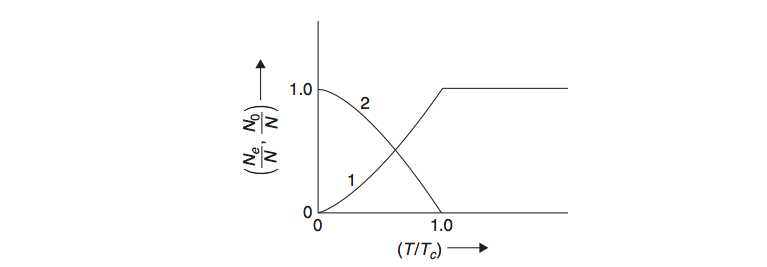
\includegraphics[width=1.0\textwidth]{Bose-N0suN.png}
	\caption{Frazione del numero di particelle nella fase normale e nella fase condensata in funzione di $T/T_c$.}
	\label{fig:n0sun}
\end{figure}
%%%%%%%%%%%%%%%%%%%%%%%%%%%%%%%%%%%%%%%%%%%%%%%%%%%%%%%%%%%%%%%%%%%%%%

È interessante anche capire la variazione di $z$ al variare di $T$, ma è più semplice considerare $z$ come funzione di $v/\lambda^3$. Ricordiamo che $v$ è il volume specifico, ossia l'inverso della densità $n$: $v = V/N$. Di conseguenza $v/\lambda^3$ è proporzionale a $T^{3/2}$. Per $T < T_c$ abbiamo visto che vale $z \simeq 1 - 1/N_0$, e poiché nel limite termodinamico $N_0$ diverge abbiamo $z \simeq 1$. Sempre dalla (\ref{eq:TCBE}) abbiamo che il valore critico di $v/\lambda^3$, cioè il valore corrispondente a $T_c$, è pari a $1/\zeta(3/2)$, che vale circa $(2.612)^{-1}$.
Per $v/\lambda^3 > (2.612)^{-1}$ il valore di $z$ è determinato implicitamente dalla relazione
\be
\gBE{3/2}(z) = \lambda^3/v < 2.612
\ee
Per valori molto grandi di $v/\lambda^3$, e cioè per valori molto piccoli di $n\lambda^3$, ritroviamo la situazione classica, ossia $z\simeq (v/\lambda^3)^{-1}$. La situazione è riassunta in figura (\ref{fig:zvsT}).
%%%%%%%%%%%%%%%%%%%%%%%%%%%%%%%%%%%%%%%%%%%%%%%%%%%%%%%%%%%%%%%%%%%%%%
\begin{figure}[!ht]
	\centering
	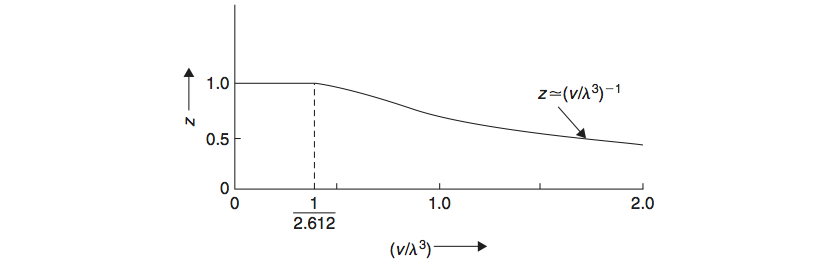
\includegraphics[width=1.0\textwidth]{Bose-zvsT.png}
	\caption{Fugacità di un gas ideale di Bose in funzione di $v/\lambda^3$.}
	\label{fig:zvsT}
\end{figure}
%%%%%%%%%%%%%%%%%%%%%%%%%%%%%%%%%%%%%%%%%%%%%%%%%%%%%%%%%%%%%%%%%%%%%%

%%%%%%%%%%%%%%%%%%%%%%%%%%%%%%%%%%%%%%%%%%%%%%%%%%%%%%%%%%%%%%%%%%%%%%
\section{Termodinamica del gas ideale di Bose}
%%%%%%%%%%%%%%%%%%%%%%%%%%%%%%%%%%%%%%%%%%%%%%%%%%%%%%%%%%%%%%%%%%%%%%

In questa sezione esamineremo le principali caratteristiche termodinamiche di un gas ideale di Bose.

%%%%%%%%%%%%%%%%%%%%%%%%%%%%%%%%%%%%%%%%%%%%%%%%%%%%%%%%%%%%%%%%%%%%%%
\subsection{La pressione}
%%%%%%%%%%%%%%%%%%%%%%%%%%%%%%%%%%%%%%%%%%%%%%%%%%%%%%%%%%%%%%%%%%%%%%

Esaminiamo il diagramma $(P,T)$, cioè la variazione di $P$ in funzione della temperatura $T$ tenendo fissata la densità $n = N/V$ (oppure $v = 1/n$) a un valore costante. Per $T \le T_c$ la pressione è data dall'eq.(\ref{eq:pintbose2}) con $z=1$. Otteniamo quindi
\be
\label{eq:pundertc}
P(T) = \dfrac{kT}{\lambda^3}\zeta(5/2)\quad\quad T \le T_c
\ee
in cui notiamo che la pressione è proporzionale a $T^{5/2}$ ed è indipendente da $V$; ciò significa che in queste condizioni il gas è {\em infinitamente comprimibile}.

Esattamente a temperatura critica, utilizziamo la (\ref{eq:nintbose3}) per scrivere
\be
\dfrac{1}{\lambda^3_c} = \dfrac{N}{V}\dfrac{1}{\zeta(3/2)}
\ee
in cui $\lambda^3_c$ è il valore di $\lambda^3$ per $T=T_c$. Sostituendo la precedente nella (\ref{eq:pundertc}) otteniamo, per la pressione a $T=T_c$:
\be
\label{eq:pattc}
P(T_c) = \dfrac{\zeta(5/2)}{\zeta(3/2)}NkT_c/V
\ee
Il rapporto $\zeta(5/2)/\zeta(3/2)$ vale circa $0.5134$, e dunque vediamo che a temperatura critica la pressione di un gas ideale di Bose è circa la metà del valore che otterremmo per un gas ideale classico.

Per $T > T_c$ il valore della pressione è dato da
\be
\label{eq:povertc}
P(T) = \dfrac{NkT}{V}\dfrac{\gBE{5/2}(z)}{\gBE{3/2}(z)}
\ee
e per eliminare $z$ allo scopo di ottenere l'equazione di stato dobbiamo risolvere la relazione implicita
\be
\gBE{3/2}(z) = n\lambda^3
\ee
A meno di non essere vicini al limite classico, in cui possiamo utilizzare l'espansione del viriale e $P$ tende asintoticamente al valore $NkT/V$, non esiste un modo semplice per esprimere la pressione e occorre adattarsi a una soluzione numerica. La situazione è riassunta in figura
(\ref{fig:PvsT}).
%%%%%%%%%%%%%%%%%%%%%%%%%%%%%%%%%%%%%%%%%%%%%%%%%%%%%%%%%%%%%%%%%%%%%%
\begin{figure}[!ht]
	\centering
	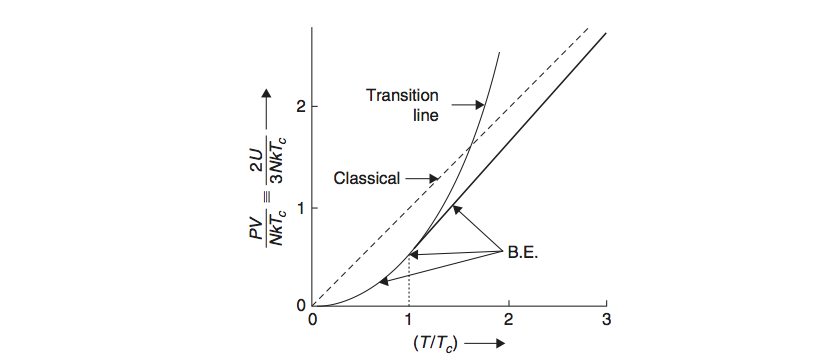
\includegraphics[width=1.0\textwidth]{Bose-PvsT.png}
	\caption{Pressione di un gas ideale di Bose in funzione di $T/T_c$.}
	\label{fig:PvsT}
\end{figure}
%%%%%%%%%%%%%%%%%%%%%%%%%%%%%%%%%%%%%%%%%%%%%%%%%%%%%%%%%%%%%%%%%%%%%%

%%%%%%%%%%%%%%%%%%%%%%%%%%%%%%%%%%%%%%%%%%%%%%%%%%%%%%%%%%%%%%%%%%%%%%
\subsection{Il calore specifico}
%%%%%%%%%%%%%%%%%%%%%%%%%%%%%%%%%%%%%%%%%%%%%%%%%%%%%%%%%%%%%%%%%%%%%%

Per calcolare il calore specifico a volume costante sotto la temperatura critica possiamo sfruttare la relazione che lega l'energia interna alla pressione e al volume:
\be
U = \dfrac{3}{2}PV
\ee
e quindi fare uso del'eq. (\ref{eq:pundertc}). Tenendo conto che $C_V = (\partial U/\partial T)_{N,V}$, possiamo scrivere
\be
\dfrac{C_V}{Nk}  = \dfrac{3V}{2N}\,\zeta(5/2)\dfrac{\de}{\de T}\bfrac{T}{\lambda^3}
= \dfrac{15}{4}\,\zeta(5/2)\dfrac{v}{\lambda^3}\quad\quad T < T_c
\ee
Vediamo quindi che quando $T$ va a zero, $C_V\to 0$ come $T^{3/2}$. 

Esattamente a $T = T_c$ abbiamo
\be
\dfrac{C_V(T_c)}{Nk} = \dfrac{15\,\zeta(5/2)}{4\,\zeta(3/2)} \simeq 1.925
\ee
che è considerevolmente più grande del valore classico pari a $3/2$.

Per $T>T_c$, ma lontani dal limite classico, tutto quel che possiamo ottenere è come al solito una relazione implicita. Utilizzando le espressioni generali per $P$ e per $N$ e la relazione che lega $U$ a $P$ otteniamo facilmente
\be
\label{eq:cvgeneric}
\dfrac{C_V}{Nk} = \dfrac{3}{2}\dfrac{\partial}{\partial T}\left(T\,\dfrac{\gBE{5/2}(z)}{\gBE{3/2}(z)}  \right)_{N,V}
\ee
il problema della quale consiste nel capire come calcolare $(\partial z/\partial T)_{N,V}$. Possiamo infatti scrivere
\be
\dfrac{C_V}{Nk} = \dfrac{3}{2}\left[\dfrac{\gBE{5/2}(z)}{\gBE{3/2}(z)}
+ T\dpard{z}{T}{N}{V}\dfrac{\partial}{\partial z}\bfrac{\gBE{5/2}(z)}{\gBE{3/2}(z)}\right]
\ee
Occupiamoci prima di tutto dell'ultima derivata. Scrivendo le funzione di Bose $\gBE{\nu}(z)$ in serie di potenze,
\be
\gBE{\nu}(z) = z + \dfrac{z^2}{2^\nu} + \dfrac{z^3}{3^\nu} + \cdots
\ee
ci accorgiamo subito che valgono le relazioni di ricorsione:
\be
\label{eq:grec}
z\dpar{\gBE{\nu}(z)}{z} = z + \dfrac{z^2}{2^{\nu-1}} + \dfrac{z^3}{3^{\nu-1}} + \cdots = \gBE{\nu-1}(z)
\ee
per cui otteniamo facilmente
\be
\label{eq:derz}
\dfrac{\partial}{\partial z}\bfrac{\gBE{5/2}(z)}{\gBE{3/2}(z)} = 
\dfrac{1}{z}\left(1 - \dfrac{\gBE{5/2}(z)\gBE{1/2}(z)}{\gBE{3/2}^2(z)} \right)
\ee
Poi notiamo che poiché $\gBE{3/2}(z) \propto T^{-3/2}$ allora
\be
\left[\dparu{T}\gBE{3/2}(z)\right]_{N,V} = -\dfrac{3}{2T}\gBE{3/2}(z)
\ee
ma avremmo ben potuto scrivere
\be
\left[\dparu{T}\gBE{3/2}(z)\right]_{N,V} = \dpard{z}{T}{N}{V}\dfrac{\partial\gBE{3/2}(z)}{\partial z} = \dpard{z}{T}{N}{V} \dfrac{1}{z}\,\gBE{1/2}(z)
\ee
in cui nell'ultimo passaggio abbiamo usato la relazione di ricorsione (\ref{eq:grec}). Otteniamo quindi
\be
\dpard{z}{T}{N}{V} = -\dfrac{3z}{2T}\dfrac{\gBE{3/2}(z)}{\gBE{1/2}(z)}
\ee
Utilizzando tutti i risultati parziali possiamo finalmente scrivere
\be
\label{eq:cvbose}
\dfrac{C_V}{Nk} = \dfrac{15\,\gBE{5/2}(z)}{4\,\gBE{3/2}(z)} - \dfrac{9\,\gBE{3/2}(z)}{4\,\gBE{1/2}(z)}
\ee
nella quale come al solito a $z$ come funzione di $T$ occorre sostituire il valore ricavato dall'equazione implitica $n\lambda^3 = \gBE{3/2}(z)$. Nel limite $z\to 1$ il secondo termine si annulla a causa della divergenza di $\gBE{1/2}(z)$ e recuperiamo il valore che avevamo calcolato per $T = T_c$; lo stesso limite che otteniamo arrivando a $T_c$ dal basso. Questo significa che il calore specifico è continuo alla transizione. La sua derivata, tuttavia, presenta una discontinuità.
%%%%%%%%%%%%%%%%%%%%%%%%%%%%%%%%%%%%%%%%%%%%%%%%%%%%%%%%%%%%%%%%%%%%%%
\begin{Exercise}
Dimostrare che per un gas di Bose ideale vale la relazione:
\be
\bfrac{\partial C_V}{\partial T}_{T\to T_c^-} -
\bfrac{\partial C_V}{\partial T}_{T\to T_c^+} =
\dfrac{27\,Nk}{16\,\pi T_c}\zeta^2(3/2)\quad\bullet
\ee
\end{Exercise}
%%%%%%%%%%%%%%%%%%%%%%%%%%%%%%%%%%%%%%%%%%%%%%%%%%%%%%%%%%%%%%%%%%%%%%
\noindent
Per $T > T_c$ il calore specifico decresce verso il suo valore limite classico:
\be
\bfrac{C_V}{Nk}_{z\to0} = \dfrac{15}{4} - \dfrac{9}{4} = \dfrac{3}{2}
\ee

%%%%%%%%%%%%%%%%%%%%%%%%%%%%%%%%%%%%%%%%%%%%%%%%%%%%%%%%%%%%%%%%%%%%%%
\subsection{Isoterme e adiabatiche}
%%%%%%%%%%%%%%%%%%%%%%%%%%%%%%%%%%%%%%%%%%%%%%%%%%%%%%%%%%%%%%%%%%%%%%

Consideriamo la variazione della pressione al variare del volume, tenendo la temperatura fissata. In questo caso otterremo la transizione per un determinato valore critico del volume, o meglio del volume specifico:
\be
v_c = \lambda^3/\zeta(3/2)
\ee
Notiamo che $v_c\propto T^{-3/2}$. Per $v < v_c$ la pressione non dipende dal volume e si riduce all'espressione (\ref{eq:pundertc}). Abbiamo quindi, ricordando che $P_0 \propto T$, 
\be
P_0v_c^{5/3} = \textrm{costante}
\ee
La regione a sinistra di questa linea, nel piano $(P,V)$, appartiene alla fase mista. La linea stessa è la linea di transizione, mentre a destra abbiamo solo la fase normale. La situazione è riassunta in figura (\ref{fig:bose-isoterme}).
%%%%%%%%%%%%%%%%%%%%%%%%%%%%%%%%%%%%%%%%%%%%%%%%%%%%%%%%%%%%%%%%%%%%%%%%
\begin{figure}[!ht]
	\centering
	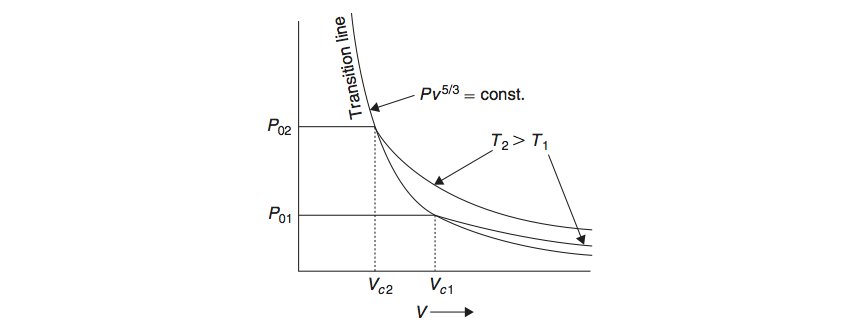
\includegraphics[width=1.0\textwidth]{Bose-isoterme.png}
	\caption{Isoterme di un gas ideale di Bose.}
	\label{fig:bose-isoterme}
\end{figure}
%%%%%%%%%%%%%%%%%%%%%%%%%%%%%%%%%%%%%%%%%%%%%%%%%%%%%%%%%%%%%%%%%%%%%%%%

Per poter studiare le adiabatiche dobbiamo trovare una formula per l'entropia del sistema: utilizzando l'espressione termodinamica
\be
G = U - TS + PV = N\mu
\ee
possiamo scrivere
\be
\dfrac{S}{Nk} = \dfrac{U + PV}{NkT} - \dfrac{\mu}{kT}
\ee
Inseriamo in questa equazione le relazioni ricavate in precedenza per $U$ e $P$, ottenendo:
\bea
\dfrac{S}{Nk} &=& \dfrac{5\,\gBE{5/2}(z)}{2\,\gBE{3/2}(z)} - \ln z\quad\quad T > T_c \nonumber\\
\dfrac{S}{Nk} &=& \dfrac{5}{2}\dfrac{v}{\lambda^3}\,\zeta(5/2)\quad\quad\quad\;\; T \le T_c
\eea
In un processo adiabatico sia $S$ sia $N$ devono rimanere costanti. La prima delle relazioni precedenti implica che sia $z$ sia $v/\lambda^3$ devono rimanere costanti per $T > T_c$. Lo stesso è vero per $T \le T_c$. Per un processo adiabatico otteniamo quindi
\bea
vT^{3/2}  &=& \textrm{costante} \nonumber\\
P/T^{5/2} &=& \textrm{costante}
\eea
ed eliminando $T$ otteniamo l'equazione per un'adiabatica:
\be
Pv^{5/3} = \textrm{costante}
\ee
Notiamo che questo risultato, che vale per ogni temperatura, è identico a quello classico, ma mentre nel caso classico l'esponente $5/3$ è il rapporto $C_P/C_V$ nel caso di Bose questo non è vero. Si può infatti dimostrare che $C_P/C_V > 5/3$ e tende al valore classico solo nel limite $n\lambda^3 \to 0$.

Infine notiamo che per $T < T_c$ possiamo scrivere
\be
S = kN_e\dfrac{5\,\zeta(5/2)}{2\,\zeta(3/2)} \propto N_e
\ee
il che equivale a dire che le particelle nel livello $\eps = 0$ non contribuiscono all'entropia.


%%%%%%%%%%%%%%%%%%%%%%%%%%%%%%%%%%%%%%%%%%%%%%%%%%%%%%%%%%%%%%%%%%%%%%%%
\section{La radiazione di corpo nero}
%%%%%%%%%%%%%%%%%%%%%%%%%%%%%%%%%%%%%%%%%%%%%%%%%%%%%%%%%%%%%%%%%%%%%%%%

La storia del corpo nero inizia intorno al 1860 quando Kirchhoff definisce che
cosa si intende per corpo nero e formula alcune leggi generali sulle sue proprietà. Kirchhoff, basandosi su dati sperimentali, arrivò a enunciare questa legge:
\begin{quote}
Per una data temperatura $T$ e una data frequenza $\nu$ della radiazione elettromagnetica, il rapporto tra potere emissivo e quello d'assorbimento è lo stesso per tutti i corpi.
\end{quote}
In formule possiamo scrivere
\be
\label{eq:funibb}
\dfrac{e(\nu,T)}{a(\nu,T)} = f(\nu,T)
\ee
in cui $f(\nu,T)$ è una funzione universale. Kirchhoff immaginò allora un oggetto il cui potere d'assorbimento fosse pari a $1$, per ogni frequenza e ogni temperatura, e chiamò quest'oggetto {\em corpo nero}. Dalla definizione (\ref{eq:funibb}) è chiaro che la funzione universale $f(\nu,T)$ coincide con la funzione $e_{\text{cn}}(\nu,T)$ d'emissione del corpo nero.

Fu lo stesso Kirchhoff a suggerire un'implementazione pratica dell'oggetto ideale {\em corpo nero}. Immaginò una cavità di volume $V$ tenuta a una temperatura costante $T$: la radiazione all'interno della cavità arriverà, prima o poi, all'equilibrio termico con le pareti del contenitore. Se ora si pratica un piccolo foro in una delle pareti del contenitore, le dimensioni del quale non compromettano l'equilibrio tra radiazione e pareti, la radiazione uscente dal foro avrà tutte le caratteristiche di una radiazione di corpo nero. In questo caso, è bene stare attenti a non confondersi, il corpo nero è rappresentato dal {\em foro}, non dall'interno del contenitore. Infatti le dimensioni del contenitore sono tali che qualsiasi tipo di radiazione entrante nel foro stesso sarà presto assorbita dalle pareti del contenitore, senza poterne riuscire (se non sotto forma di radiazione all'equilibrio termico a temperatura $T$, appunto). Il foro dunque assorbe tutta la radiazione incidente, ed emette secondo la funzione universale di corpo nero.

%%%%%%%%%%%%%%%%%%%%%%%%%%%%%%%%%%%%%%%%%%%%%%%%%%%%%%%%%%%%%%%%%%%%%%%%
\subsection{La teoria di Planck}
%%%%%%%%%%%%%%%%%%%%%%%%%%%%%%%%%%%%%%%%%%%%%%%%%%%%%%%%%%%%%%%%%%%%%%%%
Nel 1900 Planck, nel tentativo di trovare una formula che descrivesse nella maniera corretta l'enorme mole di dati sperimentali che si erano accumulati negli anni precedenti sulla radiazione di corpo nero, ipotizzò che le cariche elettriche presenti sulle pareti della cavità si muovessero come oscillatori armonici, ma con energie quantizzate: $\eps_n = n\hbar\omega$, con $n = 0,\,1,\,2,\,\ldots$, $\omega$ la frequenza (angolare) dell'oscillatore e $\hbar$ una ``costante di natura'' da determinare tramite il confronto con i dati sperimentali. Si noti l'esclusione dell'energia di punto zero, $\hbar\omega/2$, che contribuirebbe all'energia totale del sistema, nel limite termodinamico, come una costante infinita. Ma l'energia è definita a meno di una costante additiva arbitraria, e possiamo tranquillamente trascurare questo termine. Escludendo dunque l'energia di punto zero, utilizzando l'ensemble canonico e, si noti bene, la statistica di MB, l'energia media del singolo oscillatore può essere scritta come 
\be
\label{eq:ensingmod}
\langle \eps \rangle = \dfrac{\hbar\omega}{e^{\hbar\omega/kT} - 1}
\ee
All'equilibrio termico, le onde elettromagnetiche nella cavità avranno le stesse frequenze degli oscillatori armonici. La formula di Rayleigh
\be
\label{eq:rayl}
g(\omega)\de{\omega} = \dfrac{\omega^2}{\pi^2 c^3}\de{\omega}
\ee
rappresenta il numero di modi normali di vibrazione per unità di volume all'interno della cavità, nell'intervallo di frequenze $(\omega,\;\omega+\de{\omega})$. Nel ricavare la formula (\ref{eq:rayl}), in cui $c$ è la velocità della luce, Rayleigh tenne conto del fatto che le onde elettromagnetiche sono solo trasversali e hanno quindi un fattore $2$ di degenerazione.

Se dunque la (\ref{eq:ensingmod}) rappresenta l'energia del singolo modo normale di vibrazione di frequenza $\omega$, basta moltiplicare per la densità degli stati (\ref{eq:rayl}) per ottenere la densità di energia $u(\omega)\de{\omega}$ associata all'intervallo di frequenze
$(\omega,\;\omega+\de{\omega})$:
\be
\label{eq:bbplanck}
u(\omega)\de{\omega} = \dfrac{1}{\pi^2 c^3}\dfrac{\hbar\omega^3}{e^{\hbar\omega/kT} - 1}
\de{\omega}
\ee
che è esattamente la formula di Planck per la distribuzione della densità di energia della radiazione all'interno della cavità. Integrando su tutte le frequenze $\omega$ si ottiene la densità di energia totale.

%%%%%%%%%%%%%%%%%%%%%%%%%%%%%%%%%%%%%%%%%%%%%%%%%%%%%%%%%%%%%%%%%%%%%%%%
\subsection{Il punto di vista di Bose}
%%%%%%%%%%%%%%%%%%%%%%%%%%%%%%%%%%%%%%%%%%%%%%%%%%%%%%%%%%%%%%%%%%%%%%%%
Nel 1924 l'idea che il campo elettromagnetico dovesse essere quantizzato e che esistessero {\em particelle di luce} chiamate fotoni, i quanti del campo, era ormai largamente condivisa; se non altro dai fisici. Un fino ad allora oscuro ricercatore indiano, Bose, non riusciva a farsi pubblicare un articolo in cui derivava la legge di Planck a partire dal concetto di fotone, sulla base di un nuovo tipo di statistica, diversa da quella di Boltzmann. Invece di rassegnarsi all'oblio e sicuro dei suoi risultati, spedì l'articolo ad Einstein, il quale lo trovò così interessante da farlo pubblicare immediatamente. Non solo: in pochi mesi elaborò i risultati di Bose ed estese la nuova statistica a tutte le particelle che ora si chiamano bosoni.

Il lavoro di Bose e Einstein può essere rapidamente riassunto in questo modo. La famosa cavità di cui sopra è piena di particelle di massa nulla e spin pari a $1$: i fotoni. La trasversalità delle onde elettromagnetiche fa sì però che ogni fotone abbia solo $2$ possibili polarizzazioni, e non $3$. Questo gas di particelle ultrarelativistiche è all'equilibrio termico a temperatura $T$, e un singolo fotone di frequenza $\omega$ ha energia pari a $\hbar\omega$. Ci domandiamo quale sia la densità degli stati, in funzione dell'energia, per un gas ultrarelativistico. Il conto è presto fatto, perché possiamo scrivere $\eps = pc$ e usare la densità degli stati in funzione del momento, che abbiamo già calcolato:
\be
g(p)\de{p} = \dfrac{4\pi V}{h^3} p^2\de{p} = \dfrac{V}{2\pi^2\hbar^3} p^2\de{p}
\ee
Passando alle energie, possiamo scrivere
\be
g(\eps)\de{\eps} = \dfrac{V}{2\pi^2\hbar^3 c^3} \eps^2\de{\eps}
\ee
e sapendo che $\eps = \hbar\omega$ abbiamo
\be
g(\omega)\de{\omega} = \dfrac{V}{2\pi^2\hbar^3 c^3} \hbar^3\omega^2\de{\omega}
\ee
Il conto non è ancora completo, perché per ogni fotone abbiamo due possibili stati di polarizzazione, quindi dobbiamo moltiplicare il risultato per un fattore $2$, e se vogliamo ottenere la densità degli stati {\em per unità di volume} dobbiamo ancora dividere per un fattore $V$. Abbiamo dunque
\be
\label{eq:gomega}
g(\omega)\de{\omega} = \dfrac{\omega^2}{\pi^2 c^3}\de{\omega}
\ee
che senza troppe sorprese coincide con il risultato di Rayleigh, eq(\ref{eq:rayl}).

C'è un altro punto che occorre chiarire. Nel ricavare la statistica necessaria per trattare i fotoni Einstein seguì essenzialmente il procedimento che abbiamo visto nella sottosezione \ref{subsec:neps}, con un'importante differenza: non esiste un principio di conservazione del numero fotonico. I fotoni all'interno della cavità sono continuamente assorbiti e poi riemessi dalle pareti; di conseguenza non può esserci il vincolo sul numero totale $N$ di fotoni, perché tale numero è di principio indefinito. Se cade il vincolo su $N$ allora il moltiplicatore di Lagrange $\alpha$ non ha più ragione di esistere, col risultato netto che la formula per $\langle n_\eps \rangle$ diventa
\be
\label{eq:nepsfotoni}
\langle n_\eps \rangle = \dfrac{1}{e^{\eps/kT} - 1}
\ee
L'equazione precedente ci dice che per un gas di fotoni $z=1$; quindi il potenziale chimico $\mu$ è pari a 0. Allo stesso risultato si arriva con un tipo di ragionamento leggermente diverso: poiché il numero totale di particelle, per un gas di fotoni, è {\em indefinito}, il valore medio d'equilibrio, $\langle N \rangle$, deve essere ottenuto dalla condizione di minimo dell'energia libera di Von Helmoltz rispetto a una variazione di $N$ stesso, ossia
\be
\dparc{A}{N}{\langle N \rangle,\,V,\,T} = 0
\ee
L'equazione precedente implica $\mu = 0$, e quindi $z = 1$.

Usando la (\ref{eq:gomega}) e la (\ref{eq:nepsfotoni}) si ottiene immediatamente
\be
u(\omega)\de{\omega} = \dfrac{1}{\pi^2 c^3}\dfrac{\hbar\omega^3}{e^{\hbar\omega/kT} - 1}
\de{\omega}
\ee
che coincide con la formula di Planck.

%%%%%%%%%%%%%%%%%%%%%%%%%%%%%%%%%%%%%%%%%%%%%%%%%%%%%%%%%%%%%%%%%%%%%%%%
\subsection{Una visione globale è necessaria}
%%%%%%%%%%%%%%%%%%%%%%%%%%%%%%%%%%%%%%%%%%%%%%%%%%%%%%%%%%%%%%%%%%%%%%%%
Un lettore non troppo disattento potrebbe ragionevolmente chiedersi, a questo punto, come sia stato possibile, per Planck, ricavare il risultato {\em esatto} per la radiazione di corpo nero pur usando la statistica di Boltzmann e non la corretta statistica quantistica. È presto detto: gli elementi della statistica usata da Planck sono {\em i livelli di energia di un oscillatore armonico}; il numerello $n_s$ per Planck rappresenta il {\em livello d'energia} di un oscillatore armonico di energia pari a $n_s \hbar\omega$. Ma i livelli di energia sono {\em distinguibili}. Nel caso della trattazione di Bose--Einstein invece, $n_s$ rappresenta il {\em numero di fotoni} su un particolare livello di energia, e i fotoni sono {\em indistinguibili}. Anche se forniscono gli stessi risultati le due trattazioni seguono percorsi paralleli e tra di loro esistono profonde differenze concettuali.

%%%%%%%%%%%%%%%%%%%%%%%%%%%%%%%%%%%%%%%%%%%%%%%%%%%%%%%%%%%%%%%%%%%%%%%%
\begin{figure}[h!t]
  \centering
\begin{tikzpicture}[xscale=1.0,yscale=2.0]
  \draw[->] (0,-0.1) -- (0,2) node[anchor=east] {$u'(x)$};
%  \foreach \y in {1}
%    \draw (1pt,\y cm) -- (-1pt,\y cm) node[anchor=east] {$\y$};
  \draw[->] (-0.1,0) -- (10,0) node[anchor=north] {$x \equiv \hbar\omega/kT$};
  \draw[thick] plot[smooth, id=bbplanck, domain={0.01:9.0}] function{x**3/(exp(x)-1)};
  \draw[dashed,color=blue] plot[smooth, id=bbrj, domain={0.0:1.2}] function{x**2};
  \draw[dashed,color=red] plot[smooth, id=bbwien,   domain={0.0:9.0}] function{x**3*exp(-x)};
%  \draw (-1.8,0.7) node{FD};
%  \draw (-0.7,1.5) node{MB};
%  \draw (0.8,1.5)  node{BE};
\end{tikzpicture}
  \caption{La formula di Planck (linea solida) messa a confronto con quella di Wien (linea tratteggiata rossa) e con la catastrofe ultravioletta di Rayleigh--Jeans (linea tratteggiata blu).} 
  \label{fig:confrontoplanck}
\end{figure}
%%%%%%%%%%%%%%%%%%%%%%%%%%%%%%%%%%%%%%%%%%%%%%%%%%%%%%%%%%%%%%%%%%%%%%%%

In ogni caso il risultato che ormai porta giustamente il nome di Planck, può essere scritto, in forma adimensionale, come
\be
\label{eq:adimbb}
u'(x)\,\de{x} = \dfrac{x^3}{e^x - 1}\,\de{x}
\ee
in cui
\be
u'(x) = \dfrac{\pi^2 \hbar^3 c^3}{(kT)^4} u(x) \quad \text{con} \quad x = \dfrac{\hbar\omega}{kT}
\ee 
Nel limite di basse frequenze, ossia $x \ll 1$, la formula di Planck si riduce all'approssimazione classica di Rayleigh--Jeans (1905), ossia
\be
u'(x) \sim x^2
\ee
che porta al ben noto fenomeno della {\em catastrofe ultravioletta}. Va notato che la formula di Rayleigh--Jeans può essere facilmente ottenuta tramite il teorema di equipartizione, assegnando un'energia pari a $kT/2$ a ogni grado di libertà armonico del sistema. Nel limite di alte frequenze, quindi per $x \gg 1$, la formula di Planck si riduce invece alla formula di Wien (1896):
\be
u'(x) \sim x^3e^{-x}
\ee
Vedi figura \ref{fig:confrontoplanck} per un confronto visuale tra le tre espressioni.

Per la densità totale di energia nella cavità otteniamo
\be
\dfrac{U}{V} = \int_{0}^{\infty} \de{x}\, u(x) =
\dfrac{(kT)^4}{\pi^2 \hbar^3 c^3}\int_{0}^{\infty} \de{x}\,\dfrac{x^3}{e^x-1}
= \dfrac{\pi^2 k^4}{15\hbar^3 c^3}\,T^4
\ee
Se ora viene aperto un piccolo foro su una delle pareti della cavità, i fotoni effonderanno all'esterno. Il {\em rate} di effusione della radiazione, cioè della densità di energia, per unità di area dell'apertura, sarà dato dall'eq. (\ref{eq:effgen}):
\be
\label{eq:stefboltz}
R = \dfrac{U}{4V}c = \dfrac{\pi^2 k^4}{60 \hbar^3 c^2} T^4 \equiv \sigma T^4
\ee
Nella precedente, nota come equazione di Stefan--Boltzmann, $\sigma$ è nota come costante di Stefan, ed è data da
\be
\sigma = \dfrac{\pi^2 k^4}{60 \hbar^3 c^2} \simeq 5.670 \times 10^{-8} \text{\ W\,m}^{-2}
\text{\,K}^{-4}
\ee
L'equazione (\ref{eq:stefboltz}) fu ricavata da Stefan, nel 1879, a partire da dati sperimentali, e solo cinque anni dopo dedotta, sulla base di considerazioni termodinamiche, da Boltzmann.

Per proseguire lo studio termodinamico della radiazione di corpo nero sarà opportuno calcolare la funzione di granpartizione del sistema. Come al solito partiamo da
\be
\dfrac{PV}{kT} = \ln \calQ(V,T) = -\sum_\eps\ln\left(
1-e^{-\eps/kT}
\right)
\ee
nella quale abbiamo ovviamente posto $z=1$. Sostituendo l'integrale alla somma, utilizzando la densità degli stati ultrarelativistica, ossia
\be
a(\eps)\,\de{\eps} = \dfrac{8\pi V}{h^3 c^3}\eps^2\,\de{\eps}
\ee
otteniamo, dopo aver posto $x = \eps/kT$ e la solita integrazione per parti,
\be
PV = \dfrac{8\pi V}{3h^3 c^3}(kT)^4\int_0^\infty \de{x}\,\dfrac{x^3}{e^x-1}
= \dfrac{8\pi^5 V}{45 h^3 c^3}(kT)^4 = \dfrac{U}{3}
\ee
cioè un ben noto risultato. Per l'energia libera di Von Helmoltz, poiché il potenziale chimico è zero, otteniamo
\be
A = -PV = -\dfrac{U}{3}
\ee
e quindi, per l'entropia,
\be
S = \dfrac{U-A}{T} = \dfrac{4U}{3T}\propto VT^3
\ee
Per un processo adiabatico avremo
\be
VT^3 = \text{costante}
\ee
Queste considerazioni sono importanti per la termodinamica dell'universo in espansione, giacché è difficile immaginare un processo più adiabatico di questo.

Possiamo infine provare a calcolare il numero di fotoni {\em all'equilibrio} in una cavità di volume $V$ a temperatura $T$. Otteniamo
%%%%%
\be
N = \dfrac{V}{\pi^2 c^3} \int_0^\infty \de{\omega}\, 
\dfrac{\omega^2}{e^{\hbar\omega/kT}-1} = \dfrac{2V \zeta(3)(kT)^3}{\pi^2 h^3 c^3} \propto VT^3
\ee
%%%%%
Questo conto deve essere preso però con un grano di sale. Infatti la formula (\ref{eq:fluttNGran}) ci insegna che le fluttuazioni di $N$ sono proporzionali a
$(\partial P / \partial V)^{-1}$, e la derivata va fatta a $T$ costante. Ma la legge di Stefan--Boltzmann ci dice che $U/V = \sigma T^4$, quindi sappiamo che $P = 2\sigma T^4/3$;  dunque la pressione a $T$ costante non dipende dal volume. Nel caso di un gas di fotoni le fluttuazioni di $N$ sono infinite e dunque calcolare il numero medio di fotoni è un'operazione che lascia un po' il tempo che trova.

%%%%%%%%%%%%%%%%%%%%%%%%%%%%%%%%%%%%%%%%%%%%%%%%%%%%%%%%%%%%%%%%%%%%%%%%
\section{Il calore specifico dei solidi}
%%%%%%%%%%%%%%%%%%%%%%%%%%%%%%%%%%%%%%%%%%%%%%%%%%%%%%%%%%%%%%%%%%%%%%%%

Studiando il calore specifico dei solidi incontriamo un problema matematicamente molto simile a quello della radiazione di corpo nero. Stiamo qui immaginando un solido come una collezione di $N$ atomi (o molecole) che vibrano intorno alle rispettive posizioni di equilibrio a causa dell'agitazione termica.

La legge di Dulong--Petit, che è puramente sperimentale, stabilisce che il calore specifico dei solidi è indipendente dalla temperatura ed è uguale per tutti i solidi\footnote{Il calore specifico dei metalli pone una problematica particolare, che sarà discussa nel capitolo \ref{cap:fermi}.}. Il suo valore (normalizzato) è pari a
\be
\label{eq:dulpet}
\dfrac{C_V}{Nk} = 3
\ee
È notevole che tranne poche eccezioni (solidi con altissima temperatura di fusione, come il diamante) tutti i solidi, a temperature intorno a quella ambiente, rispettino questa legge sperimentale. Vediamo come possiamo comprendere questo risultato.

Sia $x_i$ una coordinata dell'$i$--mo atomo ($i = 1,\,2,\,\ldots\,,\,3N$) e $\bar x_i$ il suo valore al minimo del potenziale in cui l'atomo è immerso: in pratica la posizione di equilibrio. Scrivendo $\xi_i = x_i - \bar x_i$ otteniamo, per l'energia cinetica del sistema:
\be
K = \dfrac{1}{2}m\sum_{i=1}^{3N}\dot x_i^2 = \dfrac{1}{2}m\sum_{i=1}^{3N}\dot \xi_i^2
\ee
Inoltre espandiamo in serie di Tyalor il potenziale $\Phi(\myvec{x})$:
\bea
\Phi(\myvec{x}) &=& \Phi(\bar{\myvec{x}}) + \sum_i \dparc{\Phi}{x_i}{\myvec{x}=\bar{\myvec{x}}}
\xi_i \nonumber \\
 &+& \dfrac{1}{2}\sum_{i,j}
 \left(\dfrac{\partial^2\Phi}{\partial x_i\partial x_j}\right)_{\myvec{x}=\bar{\myvec{x}}}
 \xi_i\,\xi_j + \cdots 
\eea
Il primo termine rappresenta l'energia di punto zero del solido, quando tutti gli atomi sono a riposo, e lo denoteremo col simbolo $\Phi_0$. Il termine lineare nelle $\xi_i$ è ovviamente nullo perché la funzione $\Phi$ ha un minimo per $\myvec{x}=\bar{\myvec{x}}$, mentre il secondo termine rappresenta le componenti armoniche. Se assumiamo che le ampiezze di vibrazione non siamo molto grandi possiamo fermiarci qui nello sviluppo, ottenendo l'approssimazione armonica, cioè
\be
\Ham = \Phi_0 + \left\{
\dfrac{1}{2}m\sum_i \dot\xi_i^2 + \dfrac{1}{2}\sum_{i,j}\alpha_{ij}\xi_i\,\xi_j
\right\}
\ee
in cui abbiamo posto
\be
\alpha_{ij} = \left(\dfrac{\partial^2\Phi}{\partial x_i\partial x_j}\right)_{\myvec{x}=\bar{\myvec{x}}}
\ee
Possiamo ora introdurre una trasformazione lineare delle coordinate, da $\xi_i$ alle così dette {\em coordinate normali} $q_i$; la matrice $\alpha_{ij}$ viene diagonalizzata da questa trasformazione e otteniamo
\be
\label{eq:hamphon}
\Ham = \Phi_0 + \dfrac{1}{2}m\sum_i\left(
\dot q_i^2 + \omega_i^2 q_i^2
\right)
\ee
Le $\omega_i$ sono le frequenze caratteristiche del modi normali del sistema. Dunque in prima approssimazione il solido può essere visto come un sistema di $3N$ oscillatori armonici unidimensionali non interagenti, ognuno con la sua frequenza caratteristica $\omega_i$.

Per capire il risultato sperimentale di Dulong-Petit, immaginiamo che tutte le frequenze siano eccitate: il sistema ha dunque $6N$ gradi di libertà armonici, e per il principio di equipartizione dell'energia, trattando il sistema classicamente, abbiamo che la sua energia interna, a parte la costante $\Phi_0$, sarà data da $U = 3NkT$, da cui segue la (\ref{eq:dulpet}).

Dal punto di vista sperimentale il problema è che la legge di Dulong-Petit cessa di valere a piccole temperature; $C_V$ diventa una funzione di $T$, diversa da materiale a materiale, che però mantiene un certo grado di universalità. Infatti con l'abbassarsi della temperatura il calore specifico scende verso $0$, e quando $T\to 0$ si annulla come $T^3$.

Il problema nasce evidentemente dal fatto che a piccole temperature non possiamo più usare l'approssimazione classica per il sistema di oscillatori armonici; dobbiamo risolverci a usare il formalismo quantistico. Dal punto di vista classico i $3N$ modi normali di vibrazione corrispondono a onde di distorsione del reticolo che definisce il solido, ossia a onde sonore. Dal punto di vista quantistico questi modi saranno quantizzati, dando origine ai così detti {\em fononi}, cioè i quanti del campo vibrazionale, allo stesso modo in cui i fotoni sono i quanti del campo elettromagnetico.

Un'importante differenza rispetto al caso del corpo nero è che per i fotoni il numero di modi normali possibili è infinito, mentre per i fononi tale numero è limitato dal numero di atomi nel solido. Allo stesso modo dei fotoni, però, il numero dei fononi non è ben definito, e quindi anche i fononi hanno potenziale chimico nullo.

Per gli autovalori dell'hamiltoniana (\ref{eq:hamphon}) possiamo scrivere l'espressione
\be
E\nset = \Phi_0 + \sum_i \left(
n_i + \dfrac{1}{2}\hbar\omega_i
\right)
\ee
dove $n_i$ rappresenta il livello eccitato dell'oscillatore $i$--mo. Oppure possiamo cambiare punto di vista, e dire che $n_i$ rappresenta il numero medio di fononi nell'$i$--mo livello di energia. Considerando le cose in questo modo è immediato scrivere un'espressione per l'energia interna del sistema:
\be
U(T) = \left\{
\Phi_0 + \dfrac{1}{2}\hbar\sum_i \omega_i
\right\}
+ \sum_i \dfrac{\hbar\omega_i}{e^{\hbar\omega_i/kT} - 1}
\ee
Il termine tra parentesi graffe, che denoteremo con $\tilde\Phi_0$, rappresenta l'energia di legame del solido, mentre la somma rappresenza la parte dell'energia che dipende dalla temperatura. Otteniamo quindi facilmente
\be
\label{eq:cvsolidigen}
C_V(T) = \dfrac{\de{U}}{\de{T}} = k\sum_i \dfrac{\left(\hbar\omega_i/kT\right)^2 e^{\hbar\omega_i/kT}
}
{\left(
e^{\hbar\omega_i/kT}-1
\right)^2}
\ee
Per procedere oltre non ci resta che conoscere lo spettro di frequenze del particolare solido di cui vogliamo studiare il calore specifico. Ottenere questa informazione da principi primi è sostanzialmente impossibile; o ci limitiamo a misurarlo sperimentalmente e usare questa informazione nella formula, oppure lo calcoliamo sotto alcune ragionevoli assunzioni.

%%%%%%%%%%%%%%%%%%%%%%%%%%%%%%%%%%%%%%%%%%%%%%%%%%%%%%%%%%%%%%%%%%%%%%%%
\subsection{Il modello di Einstein}
%%%%%%%%%%%%%%%%%%%%%%%%%%%%%%%%%%%%%%%%%%%%%%%%%%%%%%%%%%%%%%%%%%%%%%%%
Il primo ad applicare la (\ref{eq:cvsolidigen}) fu Einstein nel 1907. La sua assunzione è molto cruda, ma porta a risultati in accordo almeno qualitativo con i fatti sperimentali. Einstein si è limitato ad assumere che tutte le frequenze $\omega_i$ fossero uguali. Chiamando $\omega_E$ il valore comune a tutte le $\omega_i$ otteniamo immediatamente
\be
\dfrac{C_V(T)}{Nk} = 3E(x)
\ee
in cui $E(x)$ è la così detta funzione di Einstein:
\be
\label{eq:feinsteincv}
E(x) = \dfrac{x^2e^x}{(e^x-1)^2}
\ee
con
\be
x = \dfrac{\hbar\omega_E}{kT} \equiv \dfrac{\Theta_E}{T}
\ee
Nell'ultima equazione abbiamo definito la temperatura di Einstein:
\be
\Theta_E \equiv \hbar\omega_E/k
\ee
Il limite $T \gg \Theta_E$ corrisponde a $x \ll 1$. Abbiamo quindi
\be
E(x) = \dfrac{x^2(1 + x + x^2/2 \cdots)}{x^2(1 + x/2 + x^2/6 + \cdots)^2} = 1 - \dfrac{x^2}{12} + \cdots
\ee
Nel limite di alte temperature la legge di Dulong-Petit è dunque ripristinata, con una correzione che muore quadraticamente con $\Theta_E/T$. Se invece $T \ll \Theta_E$, cioè $x \gg 1$, otteniamo
\be
\lim_{x\to \infty} E(x) \sim e^{-x} = 0
\ee
Quindi per $T\to 0$ il calore specifico scende esponenzialmente a 0. Sebbene il modello di Einstein riproduca qualitativamente l'andamento del calore specifico dei solidi, fallisce nel 
predire l'andamento come $T^3$ quando $T\to 0$.

%%%%%%%%%%%%%%%%%%%%%%%%%%%%%%%%%%%%%%%%%%%%%%%%%%%%%%%%%%%%%%%%%%%%%%%%
\subsection{Il modello di Debye}
%%%%%%%%%%%%%%%%%%%%%%%%%%%%%%%%%%%%%%%%%%%%%%%%%%%%%%%%%%%%%%%%%%%%%%%%
Il modello di Einstein fu migliorato da Peter Debye nel 1912. In primo luogo Debye ipotizzò uno spettro continuo di frequenze da $0$ a una frequenza limite $\omega_D$, detta frequenza di Debye. Il taglio è fatto in modo tale che il numero totale di modi normali di vibrazione sia pari a $3N$; in formule
\be
\int_0^{\omega_D} g(\omega) \, \de{\omega} = 3N
\ee
in cui $g(\omega)\de{\omega}$ rappresenta il numero di modi normali di vibrazione le cui frequenze cadono nell'intervallo $(\omega, \omega+\de{\omega})$; cioè in altre parole la densità degli stati necessaria per passare dalla somma sulle frequenze all'integrale.

La seconda ipotesi di Debye riguarda proprio la forma funzionale di $g(\omega)$. Debye decise di assumere la stessa forma funzionale che nel caso delle onde elettromagnetiche, con le ovvie e dovute modifiche. Prima di tutto occorre sostituire alla velocità della luce la velocità del suono nel materiale, e inoltre tenere conto che le onde sonore, oltre ad avere modi trasversi di propagazione, hanno anche modi longitudinali. Occorre anche tenere conto del fatto che i modi trasversi hanno una degenerazione pari a $2$; scrivendo $c_L$ per la velocità di propagazione dei modi longitudinali e $c_T$ per la velocità di quelli trasversi otteniamo
\be
\int_0^{\omega_D}\left(
\dfrac{\omega^2}{2\pi^2 c_L^3} + \dfrac{\omega^2}{\pi^2 c_T^3}
\right)\de{\omega} = \dfrac{3N}{V}
\ee
dalla quale ricaviamo subito
\be
\label{eq:omegaD}
\omega_D^3 = 18\pi^2 \dfrac{N}{V} \left(
\dfrac{1}{c_L^3} + \dfrac{2}{c_T^3}
\right)^{-1}
\ee
In definitiva possiamo scrivere lo spettro di frequenze di Debye come
\be
g(\omega) = \left\{
\begin{array}{ll}
\dfrac{9N\omega^2}{\omega_D^3} & \quad\quad  \text{per\ } \omega \le \omega_D \\
0 & \quad\quad \text{per\ } \omega > \omega_D
\end{array}
\right.
\ee
È da notare che sebbene il modello di Debye rappresenti un'approssimazione molto cruda dello spettro di frequenze di un solido, avvicinandosi alla realtà solo per basse frequenze, ossia nella banda acustica, nondimeno i suoi risultati sono in ottimo accordo con i dati sperimentali. A quanto pare per quantità medie, come il calore specifico, i dettagli fini dello spettro non sono molto importanti.

Applicando il modello di Debye all'eq. (\ref{eq:cvsolidigen}) e sostituendo alla somma un'integrale sulle frequenze, otteniamo
\be
\label{eq:cvdebye1}
\dfrac{C_V(T)}{Nk} = 3D(x_0)
\ee
in cui $D(x_0)$ è la funzione di Debye
\be
\label{eq:debyefunc}
D(x_0) = \dfrac{3}{x_0^3}\int_0^{x_0} \de{x} \dfrac{x^4 e^x}{(e^x - 1)^2}
\ee
con
\be
x_0 = \dfrac{\hbar\omega_D}{kT} \equiv \dfrac{\Theta_D}{T}
\ee
Integrando per parti la (\ref{eq:debyefunc}) otteniamo
\be
D(x_0) = -\dfrac{3x_0}{e^{x_0}-1} + \dfrac{12}{x_0^3}\int_0^{x_0}\de{x}\dfrac{x^3}{e^x-1}
\ee
in cui $\Theta_D = \hbar\omega_D/k$ è ovviamente la temperatura di Debye del solido. Studiamo il limite $T \gg \Theta_D$, che significa $x_0 \ll 1$. La funzione integranda può essere espansa in serie perché $x \le x_0$, e otteniamo
\bea
D(x_0) &=& -\dfrac{3}{1 + x_0/2 + x_0^2/6 + \cdots} + 
\dfrac{12}{x_0^3}\int_0^{x_0}\de{x}\,\dfrac{x^2}{1 + x/2 + + x^2/6 + \cdots} \nonumber \\
&=& -3(1 - x_0/2 + x_0^2/12 + \cdots) + \dfrac{12}{x_0^3}\,x_0^3\,(1/3 - x_0/8 + x_0^2/60 + \cdots)
\nonumber \\
&=& 1 - \dfrac{x_0^2}{20} + \cdots
\eea
Dunque nel limite $T \to \infty$ recuperiamo la legge di Dulong-Petit con correzioni che svaniscono quadraticamente con $\Theta_D/T$.

Nel limite opposto, $T \ll \Theta_D$, cioè per $x_0 \gg 1$, il primo termine a destra della (\ref{eq:debyefunc}) va a zero esponenzialmente, e il limite superiore dell'integrale può essere spostato all'infinito. Otteniamo quindi
\be
D(x_0) \simeq \dfrac{12}{x_0^3}\int_0^\infty\de{x}\,\dfrac{x^3}{e^x-1}
= \dfrac{12}{x_0^3}\,\Gamma(4)\,\zeta(4) = \dfrac{4\pi^4}{5}\left(
\dfrac{T}{\Theta_D}
\right)^3
\ee
Dunque a basse temperature ritroviamo il risultato sperimentale, cioè che il calore specifico dei solidi si annulla, per $T \to 0$, come $T^3$. Ovviamente un fit dei dati sperimentali può condurre a una stima del valore di $\Theta_D$; un'altra stima può essere fatta calcolando $\Theta_D$ sulla base delle costanti elastiche del solido, e quindi a partire da $c_L$ e $c_T$, vedi eq. (\ref{eq:omegaD}). Queste due stime sono in ottimo accordo quantitativo tra loro.




%%%%%%%%%%%%%%%%%%%%%%%%%%%%%%%%%%%%%%%%%%%%%%%%%%%%%%%%%%%%%%%%%%%%%%%%
\chapter{Sistemi ideali di Fermi--Dirac}
\label{cap:fermi}
%%%%%%%%%%%%%%%%%%%%%%%%%%%%%%%%%%%%%%%%%%%%%%%%%%%%%%%%%%%%%%%%%%%%%%%%

Nel seguito per brevità mi riferirò a un sistema di Fermi--Dirac semplicemente
come a un sistema di Fermi.

%%%%%%%%%%%%%%%%%%%%%%%%%%%%%%%%%%%%%%%%%%%%%%%%%%%%%%%%%%%%%%%%%%%%%%%%
\section{Equazioni fondamentali per un gas ideale di Fermi}
%%%%%%%%%%%%%%%%%%%%%%%%%%%%%%%%%%%%%%%%%%%%%%%%%%%%%%%%%%%%%%%%%%%%%%%%

Cominciamo con lo scrivere le relazioni per la pressione $P$ e il numero medio
di particelle $N$ che abbiamo ricavato in precedenza:
\bea
\label{eq:fermifund}
\dfrac{PV}{kT} &\equiv& \ln\calQ = \sum_\eps\ln\left(1 + \zembe\right)
\nonumber\\
N &\equiv&\sum_\eps \langle n_\eps\rangle = \sum_\eps \dfrac{1}{\zmebe+1}
\eea
Contrariamente al caso di Bose, nel caso di Fermi $z$ può assumere qualsiasi
valore: $0 \le z < \infty$. Il principio di esclusione di Pauli fa sì che in
nessun livello di energia possano accumularsi più di $g$ particelle, in cui $g$
è il fattore di degenerazione dovuto allo spin (per particelle di spin $1/2$,
come gli elettroni, $g = 2$). Quindi non ci sarà nessun fenomeno simile alla
condensazione di Bose--Einstein, e non dobbiamo preoccuparci di trattare in
maniera particolare il livello $\eps =0$, come abbiamo fatto nel caso di Bose.
Il comportamento quantistico di un gas di Fermi è completamente diverso da
quello di un gas di Bose, ma non per questo meno interessante.

Senza ripetere tutti i passaggi che portano dalle somme (\ref{eq:fermifund})
agli integrali, passaggi che sono in tutto e per tutto simili a quelli che
abbiamo visto nel capitolo precedente, a parte un segno meno di differenza,
scriviamo direttamente i risultati fondamentali:
\bea
\label{eq:fermifundint}
\dfrac{P}{kT} &=& \dfrac{g}{\lambda^3}\,\fFD{5/2}(z) \nonumber\\
\dfrac{N}{V}  &=& \dfrac{g}{\lambda^3}\,\fFD{3/2}(z)
\eea
in cui abbiamo messo ``a mano'' il fattore di degenerazione $g$ e abbiamo
introdotto le funzioni di Fermi--Dirac
\be
\label{eq:deffFD}
\fFD{\nu}(z) = \dfrac{1}{\Gamma(\nu)}\int_0^\infty\de x
\dfrac{x^{\nu-1}}{\zmex+1}
\ee
Allo stesso modo delle funzioni $\gBE{\nu}(z)$, anche le funzioni di
Fermi--Dirac ammettono uno sviluppo in serie, ma stavolta a segni alterni:
\be
\label{eq:expFD}
\fFD{\nu}(z) = z - \dfrac{z^2}{2^\nu} + \dfrac{z^3}{3^\nu} - \cdots
= \sum_{s=1}^\infty (-1)^{s-1} \dfrac{z^s}{s^\nu}
\ee
%%%%%%%%%%%%%%%%%%%%%%%%%%%%%%%%%%%%%%%%%%%%%%%%%%%%%%%%%%%%%%%%%%%%%%%%
\begin{Exercise}[title={Espansione delle funzioni di Fermi},
label={ex:fermiexp}]
Dimostrare la (\ref{eq:expFD}).

[{\em Suggerimento}\ Vedi l'esercizio equivalente per le funzioni di
Bose]$\quad\bullet$
\end{Exercise}
%%%%%%%%%%%%%%%%%%%%%%%%%%%%%%%%%%%%%%%%%%%%%%%%%%%%%%%%%%%%%%%%%%%%%%%%
\noindent
Eliminando la $z$, le (\ref{eq:fermifundint}) permettono in linea di principio
di scrivere l'equazione di stato di un gas ideale di Fermi.

%%%%%%%%%%%%%%%%%%%%%%%%%%%%%%%%%%%%%%%%%%%%%%%%%%%%%%%%%%%%%%%%%%%%%%%%
\section{Espansione del viriale}
%%%%%%%%%%%%%%%%%%%%%%%%%%%%%%%%%%%%%%%%%%%%%%%%%%%%%%%%%%%%%%%%%%%%%%%%

Analogamente al caso di Bose, possiamo scrivere, per l'energia interna,
\bea
\label{eq:defUFD}
U &=& -\bfrac{\partial\ln\calQ}{\partial\beta}_{z,V} =  
kT^2\left[\dparu{T}\bfrac{PV}{kT}\right]_{z,V} \nonumber\\
&=& kT^2 gV \fFD{5/2}(z)\dfrac{\de\lambda^{-3}}{\de T} = 
\dfrac{3}{2}kT\dfrac{gV}{\lambda^3}\fFD{5/2}(z) =
\dfrac{3}{2}NkT\dfrac{\fFD{5/2}(z)}{\fFD{3/2}(z)}
\eea
e otteniamo la solita relazione tra pressione e energia interna:
\be
\label{eq:relUPFD}
P = \dfrac{2U}{3V}
\ee

\textbf{TODO}

%%%%%%%%%%%%%%%%%%%%%%%%%%%%%%%%%%%%%%%%%%%%%%%%%%%%%%%%%%%%%%%%%%%%%%%%
\section{Il limite di degenerazione}
%%%%%%%%%%%%%%%%%%%%%%%%%%%%%%%%%%%%%%%%%%%%%%%%%%%%%%%%%%%%%%%%%%%%%%%%

Nel limite $T\to 0$, il valor medio dei numeri d'occupazione diventa
\be
\aspne = \dfrac{1}{e^{(\mu-\eps)/kT} + 1} = \left\{ \begin{array}{ll}
 1 & \eps <\mu_0\\
 0 & \eps >\mu_0
  \end{array} \right.
\ee
in cui $\mu_0$ è il valore del potenziale chimico a $T=0$. La funzione $\aspne$
diventa una funzione a gradino. Tutti i livelli di energia con $\eps < \mu_0$
sono riempiti, e tutti i livelli di energia con $\eps > \mu_0$ sono vuoti. Al
valore limite $\mu_0$, che gioca un ruolo importantissimo in molti sistemi
fisici, viene dato il nome di {\em energia di Fermi} del sistema, indicata dal
simbolo $\eps_F$. Il corrispondente valore del momento, il {\em momento di
Fermi}, si indica con $p_F$.

Per calcolare $\eps_F$, scriviamo prima di tutto l'equazione generale per il
numero medio di particelle $N$:
\be
N = \int_0^\infty \de\eps \, a(\eps) \aspne
\ee
in cui $a(\eps)$ è la solita densità degli stati (non--relativistica) del
sistema, moltiplicata per il fattore di degenerazione di spin, $g$:
\be
a(\eps) = \dfrac{gV}{h^3}2\pi(2m)^{3/2}\eps^{1/2}
\ee
Nel limite $T\to0$ $\aspne$ può essere sostituita con la funzione a gradino:
quindi
\be
\dfrac{N}{V}= \dfrac{1}{V}\int_0^{\eps_F} \de\eps\,a(\eps) = \dfrac{4\pi
g(2m)^{3/2}}{3h^3}\eps_F^{3/2}
\ee
da cui otteniamo facilmente
\be
\label{eq:computEF}
\eps_F = \dfrac{h^2}{2m}\bfrac{3n}{4\pi g}^{2/3}
\ee
e, per il momento di Fermi,
\be
\label{eq:computePF}
p_F = h\bfrac{3n}{4\pi g}^{1/3}
\ee
Per l'energia di punto zero, ossia l'energia del sistema quando $T\to 0$,
troviamo un valore diverso da zero; cosa che è nettamente in contrasto col
comportamento di un gas ideale classico, in cui l'energia interna va a zero
linearmente con la temperatura. Per essere specifici possiamo scrivere
\be
E_0 = \int_0^{\eps_F}\de\eps\,\eps\,a(\eps)
= \dfrac{2\pi g(2m)^{3/2} V}{h^3}\int_0^{\eps_F}\de\eps\,\eps^{3/2}
= \dfrac{4\pi gV(2m)^{3/2}}{5h^3}\eps_F^{5/2}
\ee
Se ora dividiamo per $N$ otteniamo
\be
\dfrac{E_0}{N} = \dfrac{3}{5}\eps_F
\ee
Utilizzando la relazione tra pressione e energia interna, che vale a qualsiasi
temperatura, otteniamo
\be
P_0 = \dfrac{2E_0}{3V} = \dfrac{2}{5}n\eps_F
\ee
Considerando che $\eps_F\propto n^{2/3}$ otteniamo che $P_0\propto n^{5/3}$.
Sembra proprio che anche allo zero assoluto il gas di Fermi continui a
esercitare una certa attività. Tutto questo è dovuto al principio di esclusione
di Pauli, quindi a un fenomeno puramente quantistico. Questo peculiare
comportamento del gas di Fermi nel limite degenere $(T\to 0)$ spiega, come
vedremo, parecchi fenomeni fisici che resterebbero altrimenti misteriosi.

Una volta definita l'energia di Fermi di un sistema, possiamo anche definire la
sua {\em temperatura} di Fermi:
\be
T_F = \eps_F/k
\ee
Quando la temperatura di un sistema costituito da fermioni è molto inferiore
alla sua temperatura di Fermi, il caso degenere costituisce una buona
approssimazione del sistema stesso.

%%%%%%%%%%%%%%%%%%%%%%%%%%%%%%%%%%%%%%%%%%%%%%%%%%%%%%%%%%%%%%%%%%%%%%%%
\section{Espansione a bassa temperatura}
%%%%%%%%%%%%%%%%%%%%%%%%%%%%%%%%%%%%%%%%%%%%%%%%%%%%%%%%%%%%%%%%%%%%%%%%

Come nel caso dei sistemi di Bose, per valori intermedi di $z$ l'unica
soluzioneconsiste nel risolvere le equazioni numericamente. Quando
$n\lambda^3\to 0$
possiamo ricorrere all'espansione del viriale, e quando $T=0$ possiamo fare i
conti esattamente, trovando una prima approssimazione nel caso di piccole
temperature. Il calcolo però del calore specifico, per esempio, richiede una
temperatura anche solo leggermente diversa da zero, per poter fare la derivata
rispetto alla temperatura stessa. Dobbiamo ricorrere a un'espansione a bassa
temperatura per poter calcolare le prime correzioni al caso degenere.

In figura (\ref{fig:nefd}) è mostrato l'andamento qualitativo di $\aspne$ per
tre valori della temperatura, $T_2 < T < T_1$ (le unità di misura sono
altamentearbitrarie). Vediamo che a temperatura $T_2$ la funzione $\aspne$ si
avvicina a
una funzione a gradino.
%%%%%%%%%%%%%%%%%%%%%%%%%%%%%%%%%%%%%%%%%%%%%%%%%%%%%%%%%%%%%%%%%%%%%%
\begin{figure}[!ht]
	\centering
	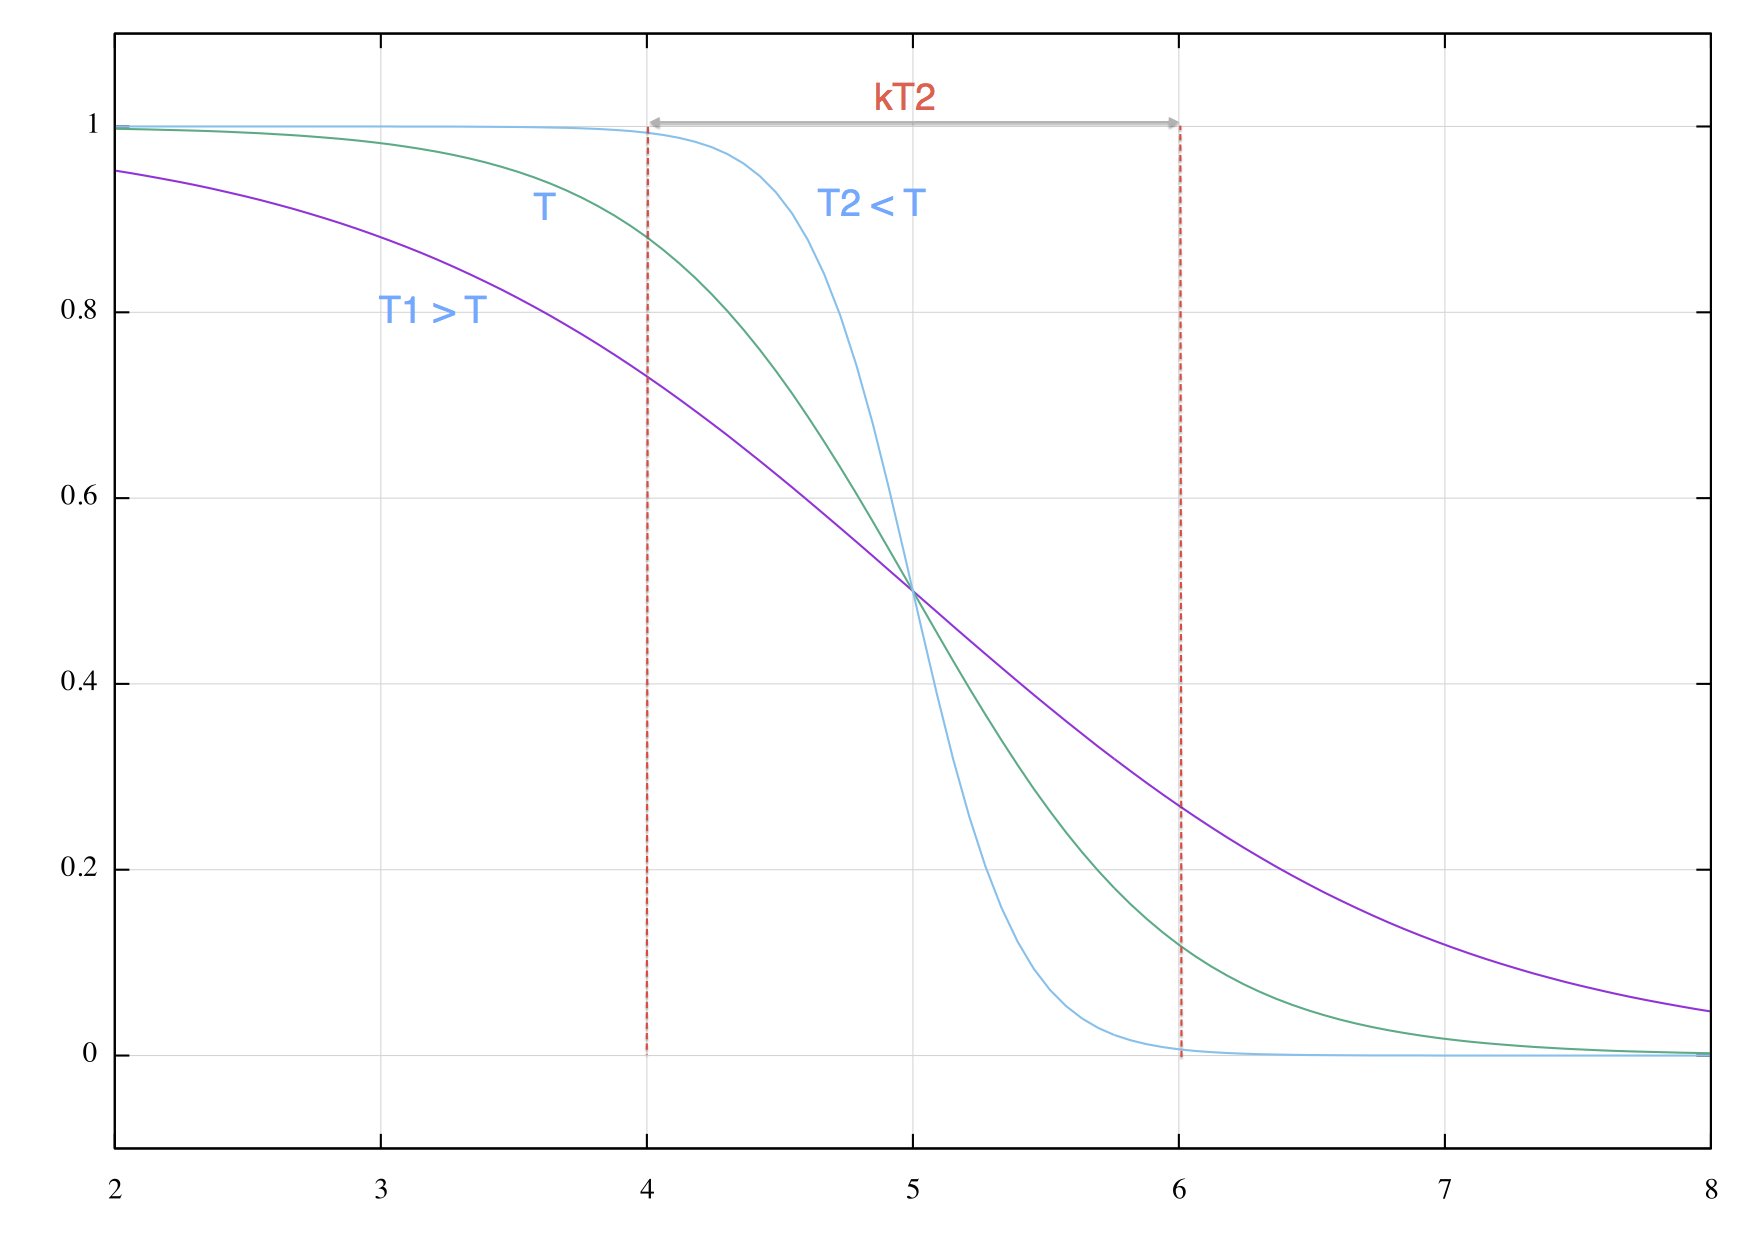
\includegraphics[width=1.0\textwidth]{nefd.png}
	\caption{Andamento qualitativo di $\aspne$ per la statistica di Fermi.}
	\label{fig:nefd}
\end{figure}
%%%%%%%%%%%%%%%%%%%%%%%%%%%%%%%%%%%%%%%%%%%%%%%%%%%%%%%%%%%%%%%%%%%%%%
\noindent
Per un valore $T$ della temperatura, la funzione $\aspne$ differisce in maniera
significativa da $0$ e da $1$ solo in un intervallo che ha un ordine di
grandezza $O(kT)$. Un argomento euristico ma profondo per capire questo
comportamento è il seguente: a temperatura $T$ l'energia termica che possiamo
fornire a una particella è proprio $O(kT)$. Se la particella si trova in un
livello di energia $\eps$ molto più basso di $\eps_F$ allora non può saltare al
livello $\eps+kT$, semplicemente perché lo trova già occupato. Solo le
particelle che si trovano a una distanza $O(kT)$ dal livello di Fermi possono
saltare per andare a occupare stati non ancora occupati, sopra il livello di
Fermi, ma a loro volta non possono andare più lontano di $O(kT)$, perché solo
quella è l'energia a disposizione. Questo argomento può essere reso più
rigoroso, come mostra il seguente esercizio.
%%%%%%%%%%%%%%%%%%%%%%%%%%%%%%%%%%%%%%%%%%%%%%%%%%%%%%%%%%%%%%%%%%%%%%
\begin{Exercise}
Si consideri un sistema costituito da fermioni a una temperatura $T \ll T_F$;
$T_F$ è la temperatura di Fermi del sistema. Si calcoli in quale intervallo la
funzione $\aspne$ è significativamente diversa da $0$ e da $1$.

\noindent
[{\em Suggerimento } Approssimare $\aspne$ con una spezzata e calcolare la
derivata prima di $\aspne$ nel punto di flesso, che corrisponde a
$\eps_F$]$\quad\bullet$
\end{Exercise}
%%%%%%%%%%%%%%%%%%%%%%%%%%%%%%%%%%%%%%%%%%%%%%%%%%%%%%%%%%%%%%%%%%%%%%

Fortunatamente le funzioni di Fermi ammettono un'espansione a bassa
temperatura.I dettagli possono essere trovati nell'appendice \textbf{TODO}. In
realtà a
temperatura $T=0$ il valore di $z$ è $\infty$. A piccole temperature le
funzioni$\fFD{\nu}(z)$ possono essere espresse come un'espansione asintotica in
potenze
di $(\,\ln z\,)^{-1}$. Per i valori di $\nu$ cui siamo interessati otteniamo
\bea
\fFD{5/2}(z) &=& \dfrac{8}{15\pi^{1/2}}(\,\ln z\,)^{5/2}\left[   
1 + \dfrac{5\pi^2}{8}(\,\ln z\,)^{-2} + \cdots
\right] \nonumber\\
\fFD{3/2}(z) &=& \dfrac{4}{3\pi^{1/2}}(\,\ln z\,)^{3/2}\left[   
1 + \dfrac{\pi^2}{8}(\,\ln z\,)^{-2} + \cdots
\right] \nonumber\\
\fFD{1/2}(z) &=& \dfrac{2}{\pi^{1/2}}(\,\ln z\,)^{1/2}\left[   
1 - \dfrac{\pi^2}{24}(\,\ln z\,)^{-2} + \cdots
\right]
\eea
Armati di queste espansioni otteniamo facilmente
\be
\dfrac{N}{V} = \dfrac{4\pi g}{3}\bfrac{2m}{h^2}^{3/2}(\,kT\ln z\,)^{3/2}\left[ 
1 + \dfrac{\pi^2}{8}(\,\ln z\,)^{-2} + \cdots\right]
\ee
che nell'approssimazione zero ci dà
\be
kT\ln z \equiv \mu \simeq \bfrac{3n}{4\pi g}\dfrac{h^2}{2m}
\ee
risultato identico, ovviamente, a quello del caso degenere: $\mu_0 = \eps_F$.
All'ordine successivo otteniamo
\be
\label{eq:muexpf}
kT\ln z \equiv \mu \simeq \eps_F \left[ 
1 - \dfrac{\pi^2}{12}\bfrac{kT}{\eps_F}^{2}\right]
\ee
Per la densità di energia interna abbiamo
\be
\dfrac{U}{N} = \dfrac{3}{5}(\,kT\ln z\,)\left[ 
1 + \dfrac{\pi^2}{2}(\,\ln z\,)^{-2} + \cdots\right]
\ee
che con l'aiuto della (\ref{eq:muexpf}) diventa
\be
\label{eq:ufd}
\dfrac{U}{N} = \dfrac{3}{5}\eps_F\left[ 
1 + \dfrac{5\pi^2}{12}\bfrac{kT}{\eps_F}^{2} + \cdots\right]
\ee
e da questa ricaviamo subito la pressione:
\be
P = \dfrac{2U}{3V} = \dfrac{2}{5}n\eps_F\left[ 
1 + \dfrac{5\pi^2}{12}\bfrac{kT}{\eps_F}^{2} + \cdots\right]
\ee
Infine, derivando la (\ref{eq:ufd}) rispetto a $T$ tenendo $z$, $N$ e $V$
costanti, otteniamo
\be
\dfrac{C_V}{Nk} = \dfrac{\pi^2}{2}\dfrac{kT}{\eps_F} + \cdots =
\dfrac{\pi^2}{2}\dfrac{T}{T_F} + \cdots
\ee
Vediamo quindi che per gas ideali di Fermi il calore specifico va a zero
linearmente con $T/T_F$. Questo risultato ci sarà molto utile in seguito, per
spiegare il calore specifico dei metalli.

%%%%%%%%%%%%%%%%%%%%%%%%%%%%%%%%%%%%%%%%%%%%%%%%%%%%%%%%%%%%%%%%%%%%%%
\section{Fenomeni magnetici in un gas di Fermi ideale}
%%%%%%%%%%%%%%%%%%%%%%%%%%%%%%%%%%%%%%%%%%%%%%%%%%%%%%%%%%%%%%%%%%%%%%

È interessante studiare il comportamento dei fermioni in presenza di un campo
magnetico. Ci aspettiamo che la statistica di Fermi--Dirac modifichi in maniera
sostanziale i risultati che abbiamo ottenuto studiando, per esempio, il
paramagnetismo con la statistica di Maxwell--Boltzmann. Le nostre aspettative
non andranno deluse. Abbiamo visto che classicamente troviamo la legge di
Curie,ossia il fatto che la suscettività magnetica è proporzionale a $T^{-1}$
nel
limite di alte temperature; a basse temperature otteniamo invece una
saturazionemagnetica completa. Sperimentalmente questo non è quel che si
osserva. Gli
elettroni in banda di conduzione nei metalli alcalini dovrebbero formare nel
metallo, in prima approssimazione, un gas ideale; quel che si osserva, invece
della situazione classica, è un paramagnetismo estremamente debole che non
mostra saturazione a basse temperature. Questo fenomeno è stato compreso da
Pauli nel 1927 sulla base della statistica di Fermi--Dirac.

Un altro fenomeno che è completamente incomprensibile dal punto di vista
classico è il diamagnetismo, ossia il fatto che un gas di elettroni acquisisce
una magnetizzazione che è di verso contrario a quello del campo magnetico.
Questo fenomeno fu spiegato da Landau nel 1930, e la spiegazione ha a che fare
con la quantizzazione delle orbite degli elettroni in un campo magnetico
esternoperpendicolare al piano dell'orbita stessa. Questo porta a una
suscettività
negativa. Per comprendere il comportamento magnetico di alcuni materiali è
dunque necessario prendere in considerazione entrambi gli effetti.

%%%%%%%%%%%%%%%%%%%%%%%%%%%%%%%%%%%%%%%%%%%%%%%%%%%%%%%%%%%%%%%%%%%%%%
\subsection{Paramagnetismo di Pauli}
%%%%%%%%%%%%%%%%%%%%%%%%%%%%%%%%%%%%%%%%%%%%%%%%%%%%%%%%%%%%%%%%%%%%%%

Sia $m$ la massa di una particella di spin $1/2$, $\musb$ il suo momento
magnetico intrinseco e $\mathbf{B}$ un campo magnetico esterno. L'energia di
singola particella, in questo caso, è data da
\be
\eps = \dfrac{p^2}{2m} - \musb \cdot \mathbf{B}
\ee
Il vettore $\musb$ sarà o parallelo o antiparallelo al vettore $\mathbf{B}$.
Nelgas troveremo dunque due gruppi di particelle:
\begin{enumerate}
\item[i)] il gruppo di particelle con $\musb$ parallelo a $\mathbf{B}$ ed
energia $\eps = \dfrac{p^2}{2m} - \mu^*B$;
\item[ii)] il gruppo di particelle con $\musb$ antiparallelo a $\mathbf{B}$ ed
energia $\eps = \dfrac{p^2}{2m} + \mu^*B$.
\end{enumerate}
A $T=0$ tutti i livelli di energia fino a $\eps_F$ saranno pieni, mentre tutti
ilivelli con energia superiore saranno vuoti. Di conseguenza l'energia {\em
cinetica} del primo gruppo di particelle andrà da $0$ a $(\eps_F + \mu^*B)$,
mentre quella del secondo andrà da $0$ a $(\eps_F - \mu^*B)$.

Chiamiamo $N^+$ il numero di particelle nel primo gruppo e $N^-$ il numero di
particelle nel secondo gruppo; usando le formule standard del caso
completamentedegenere otteniamo
\bea
N^+ &=& \dfrac{4\pi V (2m)^{3/2}}{3h}\left[ \eps_F + \mu^*B \right]^{3/2}
\nonumber \\
N^- &=& \dfrac{4\pi V (2m)^{3/2}}{3h}\left[ \eps_F - \mu^*B \right]^{3/2}
\eea
Il momento magnetico netto posseduto dal sistema sarà
\bea
M &=& \mu^* (N^+ - N^-) \nonumber \\
  &=& \dfrac{4\pi \mu^* V (2m\eps_F)^{3/2}}{3h}\left\{
\left[ 1 + \dfrac{\mu^*B}{\eps_F} \right]^{3/2} - 
\left[ 1 - \dfrac{\mu^*B}{\eps_F} \right]^{3/2}
\right\}
\eea
Per campo debole possiamo espandere $(1 \pm x)^\alpha \simeq 1 \pm \alpha x$
ottenendo
\be
\chi_0 = \lim_{B \to 0} \dfrac{M}{VB} = \dfrac{4\pi \mu^{*2} V
(2m)^{3/2}\eps_F^{1/2}}{h^3}
\ee
Ricordando l'espressione (\ref{eq:computEF}) possiamo scrivere
\be
\chi_0 = \dfrac{3}{2} n \mu^{*2} / \eps_F
\ee
in cui $n = N/V$; dunque una suscettività costante e soppressa da $\eps_F$.

Per ottenere un'espressione (approssimata) di $\chi$ valida a tutte le
temperature dobbiamo seguire una via un po' tortuosa. Chiamiamo
$n^+_{\mathbf{p}}$ il numero di particelle con momento $\mathbf{p}$ e momento
magnetico parallelo al campo magnetico, e $n^-_{\mathbf{p}}$ il numero di
particelle con momento $\mathbf{p}$ e momento magnetico antiparallelo al campo
magnetico. In virtù della statistica di Fermi devono ovviamente valere i
vincoli\be
\label{eq:npnm}
n^+_{\mathbf{p}}\;,\, n^-_{\mathbf{p}} = 0 \; \mathrm{o} \; 1
\ee
e
\be
\label{eq:NpNm}
\sum_{\mathbf{p}} n^+_{\mathbf{p}} + \sum_{\mathbf{p}}n^-_{\mathbf{p}} = N^+ +
N^- = N
\ee

L'energia totale del sistema sarà evidentemente data da
\bea
E_n &=& \sum_{\mathbf{p}} \left[
\left( \dfrac{p^2}{2m} - \mu^* B \right) n^+_{\mathbf{p}} +
\left( \dfrac{p^2}{2m} + \mu^* B \right) n^-_{\mathbf{p}}
\right] \nonumber \\
&=& \sum_{\mathbf{p}} \left[
\left( n^+_{\mathbf{p}} + n^-_{\mathbf{p}} \right) \dfrac{p^2}{2m}
\right] - \mu^* B (N^+ - N^+)
\eea
e la funzione di partizione del sistema sarà
\be
Q(N) = \sideset{}{'}\sum_{\{n^+_{\mathbf{p}}\}\{n^-_{\mathbf{p}}\}} e^{-\beta
E_n}
\ee
in cui l'apice sulla somma ci ricorda che la somma stessa, su tutti i possibili
stati, è sottoposta ai vincoli (\ref{eq:npnm}) e (\ref{eq:NpNm}). Per calcolare
la funzione di partizione $Q_N$, prima di tutto fissiamo un valore arbitrario
per il numero $N^+$; ciò fissa automaticamente anche $N^-$. A questo punto
sommiamo su tutti i possibili valori di $n^+_{\mathbf{p}}$ e $n^+_{\mathbf{p}}$
che sono conformi, oltre al vincolo (\ref{eq:npnm}), anche al valore fissato di
$N^+$ e $N^-$. Infine sommiamo su tutti i possibili valori di $N^+$, cioè da
$0$a $N$. Abbiamo dunque
\bea
\label{eq:QNPauliParam}
Q(N) &=& \sum_{N^+=0}^N
e^{\beta\mu^* B(2N^+ - N)}  \times \nonumber \\
&\ & \left[
\sideset{}{''}\sum_{\{n^+_{\mathbf{p}}\}}
\exp\left(-\beta\sum_{\mathbf{p}}\dfrac{p^2}{2m}n^+_{\mathbf{p}}\right)
 \sideset{}{'''}\sum_{\{n^-_{\mathbf{p}}\}}
\exp\left(-\beta\sum_{\mathbf{p}}\dfrac{p^2}{2m}n^-_{\mathbf{p}}\right)
\right]
\eea
in cui la somma $\sum''$ è soggetta al vincolo 
$\sum_{\mathbf{p}}n^+_{\mathbf{p}} = N^+$
mentre la somma $\sum'''$ al vincolo
$\sum_{\mathbf{p}}n^-_{\mathbf{p}} = N-N^+$.

Consideriamo ora un gas ideale di $N_0$ particelle di massa $m$ che obbediscono
alla statistica di Fermi--Dirac; queste particelle sono però ``senza spin''.
Anche se questa è chiaramente una {\em finzione}, nessuno potrà impedirci di
fare i conti. Per la funzione di partizione $Q_0(N_0)$ di questo sistema
fittizio otteniamo
\be
Q_0(N_0) = \sideset{}{'}\sum_{n_{\mathbf{p}}}
\exp \left(
-\beta \sum_{\mathbf{p}} \dfrac{p^2}{2m}n_{\mathbf{p}}
\right) \equiv e^{-\beta A_0(N_0)}
\ee
in cui per definizione $A_0(N_0)$ è l'energia libera del sistema stesso. Risulta evidente che l'eq. (\ref{eq:QNPauliParam}) può essere riscritta come
\be
Q(N) = e^{-\beta\mu^* BN}\sum_{N^+=0}^N
\left[
e^{2\beta\mu^* BN^+} Q_0(N^+) Q_0(N-N^+)
\right]
\ee
dalla quale ricaviamo subito
\bea
&&\dfrac{1}{N}\ln Q(N) = -\beta \mu^* B \nonumber \\
&+& \dfrac{1}{N}\ln \sum_{N^+=0}^N \exp
\left\{
2\beta \mu^* B N^+ - \beta A_0(N^+) - \beta A_0(N-N^+)
\right\}
\eea
Come abbiamo più volte fatto in passato, approssimiamo il logaritmo della somma con il logaritmo del termine più grande della somma stessa; l'errore {\em relativo} commesso, nel limite termodinamico, risulta trascurabile. Il termine più grande della somma si otterrà per un valore di $N^+$ pari a $\bar{N}^+$, e per trovarlo massimizziamo rispetto a $N^+$; otteniamo
\be
2 \mu^* B - 
\dparc{A_0(N^+}{N^+}{N^+=\bar{N}^+} -
\dparc{A_0(N-N^+}{N^+}{N^+=\bar{N}^+}
= 0
\ee
cioè
\be
\label{eq:mu0PauliParam}
\mu_0(\bar{N}^+) - \mu_0(N-\bar{N}^+) = 2 \mu^* B
\ee
in cui evidentemente $\mu_0(N_0)$ è il potenziale chimico del sistema fittizio di $N_0$ fermioni senza spin. Per la magnetizzazione totale, per definizione, avremo
\be
M = \mu^*
\left(
\bar{N}^+ - \bar{N}^-
\right) = \mu^*
\left(
2\bar{N}^+ - N
\right)
= \mu^* N r
\ee
in cui abbiamo introdotto il parametro $r \equiv 2\bar{N}^+/N - 1$, con $0 \le r \le 1$. L'equazione (\ref{eq:mu0PauliParam}) diventa
\be
\label{eq:mu0rPP}
\mu_0
\left(
\dfrac{1+r}{2}N
\right)
-
\mu_0
\left(
\dfrac{1-r}{2}N
\right)
=
2 \mu^* B
\ee
Se il campo magnetico è nullo, allora anche $r$ sarà nullo, perché in assenza di campo magnetico dovremo avere, in media, $\bar{N}^+ = \bar{N}^-$. Quindi per campo magnetico piccolo possiamo espandere intorno a $r=0$:
\bea
\mu_0
\left(
\dfrac{1+r}{2}N
\right)
\simeq \mu_0(N/2) + \dfrac{r}{2}\dparc{\mu_0(xN)}{x}{x=1/2} + \cdot \nonumber \\
\mu_0
\left(
\dfrac{1-r}{2}N
\right)
\simeq \mu_0(N/2) - \dfrac{r}{2}\dparc{\mu_0(xN)}{x}{x=1/2} + \cdot
\eea
e sottraendo membro a membro otteniamo, ricordando la (\ref{eq:mu0rPP}),
\be
r \simeq \dfrac{2\mu^* B}{\dparc{\mu_0(xN)}{x}{x=1/2}}
\ee
Dunque per campo debole la suscettività per unità di volume è
\be
\chi = \dfrac{M}{VB} = \dfrac{\mu^* N r}{V B} = \dfrac{2n\mu^*}{\dparc{\mu_0(xN)}{x}{x=1/2}}
\ee
Questo è il risultato che cercavamo, valido per ogni temperatura.

Per $T\to 0$, il potenziale chimico del sistema fittizio è l'energia di Fermi di detto sistema:
\be
\mu_0(xN) =
\left(
\dfrac{3xN}{4\pi V}
\right)^{2/3}\dfrac{h^2}{2m}
\ee
da cui ricaviamo facilmente
\be
\dparc{\mu_0(xN)}{x}{x=1/2} = \dfrac{2^{4/3}}{3}
\left(
\dfrac{3N}{4\pi V}
\right)^{2/3}\dfrac{h^2}{2m}
\ee
D'altra parte sappiamo ben scrivere l'energia di Fermi per il sistema fisico sotto esame:
\be
\eps_F =
\left(
\dfrac{3N}{8\pi V}
\right)^{2/3}\dfrac{h^2}{2m}
\ee
e con l'aiuto delle ultime due equazioni ricaviamo
\be
\chi_0 = \dfrac{3}{2} n \mu^{*2} / \eps_F
\ee
in completo accordo con nostro precedente risultato a $T = 0$. 

%%%%%%%%%%%%%%%%%%%%%%%%%%%%%%%%%%%%%%%%%%%%%%%%%%%%%%%%%%%%%%%%%%%%%%
\subsection{Diamagnetismo di Landau}
%%%%%%%%%%%%%%%%%%%%%%%%%%%%%%%%%%%%%%%%%%%%%%%%%%%%%%%%%%%%%%%%%%%%%%

Per quest'anno il diamagnetismo di Landau e l'effetto termoionico non sono in programma. Questo non vi impedisce di portarli come argomento a piacere.


\chapter{Il modello di Ising}

L'Hamiltoniana del modello di Ising è data da
%---
\be
\Ham = -J\sum_{\langle i,j\rangle}\sigma_{i}\sigma_{j} - h\sum_{i}\sigma_{i}
\ee
%---
in cui:
\begin{itemize}
\item gli indici $i,j$ sono interi che etichettano i siti di un reticolo;
\item $\langle i,j\rangle$ significa somma su $i$ e $j$ primi vicini;
\item $\sigma_{i}$ è una variabile di spin, il cui valore può essere $\pm 1$;
\item $J$ è il parametro di interazione, e se $J > 0$ spin primi vicini tendono
a stare allineati (la configurazione è energeticamente favorita);
\item $h$ è un eventuale campo magnetico esterno.
\end{itemize}

Questo modello è un ottimo punto di partenza per studiare il comportamento
critico (cioè alla transizione) di materiali ferromagnetici. Tali materiali
mostrano una magnetizzazione spontanea se la temperatura d'equilibrio è
inferiore a una temperatura critica $T_{c}$, detta {\em temperatura di Curie}.

Nel linguaggio del nostro modello la magnetizzazione totale $M$ è data da
%---
\be
M = \langle \sum_{i}\sigma_{i}\rangle
\ee
%---
Se il sistema è composto da $N$ spin possiamo definire una densità di
magnetizzazione $m = M/N$, che continueremo a chiamare magnetizzazione. Il
valore d'aspettazione è definito nell'ambito del formalismo canonico:
%---
\be
M =
\frac{1}{Q}\sum_{[\sigma]}\left(\sum_{i}\sigma_{i}\right)e^{-\beta\Ham[\sigma]}
\ee
%---
in cui
%---
\be
\sum_{[\sigma]} = \sum_{\sigma_{1} = \pm 1}\sum_{\sigma_{2} = \pm
1}\cdots\sum_{\sigma_{N} = \pm 1}
\ee
%---
Si vede subito che
%---
\be
M = \frac{1}{\beta}\frac{\partial \ln Q}{\partial h}
\ee
%---
e $Q$ è ovviamente la funzione di partizione del sistema:
%---
\be
Q = \sum_{[\sigma]}e^{-\beta\Ham[\sigma]}
\ee
%---
Pur nella sua semplicità, il modello di Ising è stato risolto in maniera esatta
solo in dimensione $D = 1$ e in dimensione $D = 2$ ma solamente per $h=0$.

\section{Il modello in una dimensione}

In $D = 1$ il modello di Ising può essere risolto in molti modi. Ci limiteremo a illustrare i due più interessanti: l'espansione esatta ad alta temperatura e il
metodo della matrice di trasferimento.

\subsection{Espansione ad alta temperatura}

Poniamo il campo magnetico $h=0$ e imponiamo condizioni periodiche al contorno:
$\sigma_{N+1} = \sigma_{1}$. Possiamo scrivere
\be
\Ham = -J\sum_{i=1}^N \sigma_{i}\sigma_{i+1}
\ee
Utilizziamo l'identità
\bea
\exp(\beta J \sigma_i \sigma_{i+i}) &=&
\cosh(\beta J) + \sigma_i \sigma_{i+i} \sinh(\beta J) \nonumber \\
&=& \cosh(\beta J) \left[ 1 + \sigma_i \sigma_{i+i} t \right]
\eea
con $t \equiv \tanh(\beta J)$. Per la funzione di partizione possiamo dunque
scrivere
\be
Q = \left[ \cosh(\beta J) \right]^N \sum_{[\sigma]} \prod_{i=1}^N
(1 + \sigma_i \sigma_{i+i} t)
\ee
Scrivendo esplicitamente la produttoria,
\be
Q = \left[ \cosh(\beta J) \right]^N \sum_{[\sigma]} (1+\sigma_1\sigma_2
t)(1+\sigma_2\sigma_3 t) \cdots (1+\sigma_N\sigma_1 t)
\ee
vediamo che possiamo riscrivere la produttoria stessa come una serie in potenze di $t$ (per questo è un'espansione ad alta temperatura, perché se $T\to\infty$ allora $t\to 0$):
\bea
Q &=& \left[ \cosh(\beta J) \right]^N \sum_{[\sigma]} 
[
1 + t(\sigma_1\sigma_2 + \sigma_2\sigma_3 + \cdots)  \nonumber\\
&& + t^2 (\sigma_1\sigma_3 + \sigma_1\sigma_2\sigma_3\sigma_4 + \cdots)
+ \cdots + t^N
]
\eea
Quando sommiamo su $\sigma_i = \pm 1$, tutti i termini che contengono $\sigma_i$ si annullano nella somma. Considerando che il numero totale di configurazioni è pari a $2^N$ otteniamo
\be
Q = \left[ 2\cosh(\beta J) \right]^N (1 + t^N)
\ee
Poiché $t$ è sempre minore di $1$, nel limite termodinamico il termine $t^N$ scompare. Otteniamo quindi, per l'energia libera,
\be
A = -kT\ln Q = -Nkt \ln[2\cosh(J/kT)]
\ee

\subsection{La matrice di trasferimento}

Con condizioni periodiche al contorno e $h \ne 0$ possiamo riscrivere
l'Hamiltoniana in maniera simmetrica:
%---
\be
\Ham = -J\sum_{i}\sigma_{i}\sigma_{i+1} -
\frac{h}{2}\sum_{i}(\sigma_{i}+\sigma_{i+1})
\ee
%---
Introducendo i vettori di stato $|\sigma_{i}\rangle$ e l'operatore $\hat{P}$,
con elementi di matrice uguali a
%---
\be
\langle\sigma_{i}| \hat{P} |\sigma_{i+1}\rangle =
\exp\left\{\beta[J\sigma_{i}\sigma_{i+1} + h(\sigma_{i}+\sigma_{i+1})/2]
\right\}
\ee
%---
possiamo riscrivere la funzione di partizione in questo modo:
%---
\be
Q = \sum_{\sigma_{1} = \pm 1}\sum_{\sigma_{2} = \pm 1}\cdots\sum_{\sigma_{N} =
\pm 1}
\langle\sigma_{1}| \hat{P} |\sigma_{2}\rangle\langle\sigma_{2}| \hat{P}
|\sigma_{3}\rangle\cdots\langle\sigma_{N}| \hat{P} |\sigma_{1}\rangle
\ee
%---
Poiché vale la relazione di completezza
%---
\be
\sum_{\sigma_{i}=\pm 1}|\sigma_{i}\rangle\langle\sigma_{i}| = 1\quad \forall i
\ee
%---
otteniamo facilmente
%---
\be
Q = \sum_{\sigma_{1}=\pm 1}\langle\sigma_{1}| \hat{P}^{N} |\sigma_{1}\rangle =
\mbox{Tr}(\hat{P}^{N}) = \lambda_{1}^{N} + \lambda_{2}^{N}
\ee
%---
in cui $\lambda_{1}$ e $\lambda_{2}$ sono gli autovalori della matrice
%---
%\myformula{-}{
%P = \startmatrix[left={\left(\,},right={\,\right)}]
%\NC e^{\beta(J+h)} \NC e^{-\beta J}    \NR
%\NC e^{-\beta J}   \NC e^{\beta(J-h)}  \NR
%\stopmatrix
%}
%---
L'equazione quadratica che li definisce è:
%---
\be
\lambda^{2} - \lambda e^{\beta J}(e^{\beta h} + e^{-\beta h}) + e^{2\beta J} - e^{-2\beta J}= 0
\ee
%---
e con un po' di manipolazione algebrica troviamo
%---
\be
\lambda = e^{\beta J} \cosh(\beta h) \pm \sqrt{e^{-2\beta J} + e^{2\beta
J}\sinh^{2}(\beta h)}
\ee
%---
Poiché $\lambda_{2} < \lambda_{1}$ possiamo scrivere 
%---
\be
Q = \lambda_{1}^{N}[1+(\lambda_{2}/\lambda_{1})^{N}]
\ee
%---
e quindi nel limite termodinamico ($N\to\infty$) conta solo l'autovalore più
grande. Quindi per l'energia libera di Von Helmholtz otteniamo
%---
\be
A = -\frac{1}{\beta}\ln Q \simeq -\frac{N}{\beta}\ln\lambda_{1}
\ee
%---
e per la magnetizzazione otteniamo
%---
\be
M = -\left(\frac{\partial A}{\partial h}\right)_{T} = \frac{N\sinh(\beta h)}
{\sqrt{e^{-4\beta J}+\sinh^{2}(\beta h)}}
\ee
%---
Vediamo subito che se $h=0$ la magnetizzazione è nulla per tutte le temperature
maggiori di zero. Questo significa che in una dimensione il modello di Ising non presenta la transizione di fase ferromagnetica.

Se $J=0$ ritroviamo il risultato paramagnetico, ossia
%---
\be
M = N\tanh(\beta h)
\ee
%---

\section{Approssimazione di campo medio}

Il conto esatto in due dimensioni risulta abbastanza complicato. Come prima
approssimazione, valida in dimensione $D$ qualsiasi, partiamo dal cosiddetto
{\em campo medio}, un approccio variazionale basato sulla minimizzazione
dell'energia libera. Ciò che si minimizza, però, non è la {\em vera} energia
libera, ma un funzionale ``energia libera'' che deriva da una distribuzione di
probabilità fattorizzata. Scriviamo cioè
%---
\be
\rho_{\mbox{mf}}[\sigma] = \prod_{i}\rho_{i}(\sigma_{i})
\ee
%---
in cui
%---
\be
\rho_{i}(\sigma) = \frac{1+m_{i}}{2}\delta_{\sigma,1} +
\frac{1-m_{i}}{2}\delta_{\sigma,-1}
\ee
%---
in cui $m_{i}$ è il parametro su cui effettueremo la minimizzazione. Il suffisso``mf'' sta per {\em mean field}, ossia campo medio. La $\rho$ di campo medio è
normalizzata a 1:
%---
\be
\sum_{\sigma_{i}=\pm 1}\rho_{i}(\sigma_{i}) = \frac{1+m_{i}}{2} +
\frac{1-m_{i}}{2} = 1
\ee
%---
e quindi
%---
\be
Q_{\mbox{mf}} = \sum_{[\sigma]}\rho_{\mbox{mf}} = 1
\ee
%---
e otteniamo subito
%---
\be
\langle A[\sigma_{i}] \rangle_{\mbox{mf}} = \frac{1+m_{i}}{2}A(1) +
\frac{1-m_{i}}{2}A(-1)
\ee
%---
In particolare l'ultima equazione implica
%---
\be
\langle \sigma_{i} \rangle_{\mbox{mf}} = \frac{1+m_{i}}{2} - \frac{1-m_{i}}{2}A
= m_{i}
\ee
%---
e quindi $m_{i}$ è proprio la magnetizzazione locale nel punto $i$. Nel seguito
per semplicità ometteremo il sottoscritto ``mf''. La fattorizzazione della
$\rho$ implica
%---
\be
\aspetta{AB} = \aspetta{A}\aspetta{B}
\ee
%---
in modo tale che possiamo immediatamente scrivere
%---
\be
U = \aspetta{\Ham} = -J\sum_{\langle i,j\rangle}m_{i}m_{j} - h\sum_{i}m_{i}
\ee
%---
Per l'entropia otteniamo invece
%---
\be
S = -\aspetta{\ln\rho} = -\sum_{i}\aspetta{\ln\rho_{i}} = -\sum_{i}s_{i}
\ee
%---
in cui
%---
\be
s_{i} = \frac{1+m_{i}}{2}\ln\left(\frac{1+m_{i}}{2}\right) +
\frac{1-m_{i}}{2}\ln\left(\frac{1-m_{i}}{2}\right)
\ee
%---
Definiamo un funzionale $\Phi$ tale che se $\rho$ fosse la giusta distribuzione
di Boltzmann allora $\Phi$ sarebbe l'energia libera:
%---
\be
\Phi = U - \frac{1}{\beta}S = -J\sum_{\langle i,j\rangle}m_{i}m_{j} -
h\sum_{i}m_{i}-\frac{1}{\beta}\sum_{i}s_{i}
\ee
%---
in cui abbiamo posto $k=1$, e quindi la temperatura ha le stesse dimensioni
fisiche di un'energia. Imponiamo ora la condizione di estremizzazione, ossia
deriviamo $\Phi$ rispetto a $m_{i}$ e imponiamo che la derivata sia nulla. Per
semplificare i conti scriviamo
%---
\be
-J\sum_{\langle i,j\rangle}m_{i}m_{j} \equiv -\sum_{i,j}J_{ij}m_{i}m_{j}
\ee
%---
in cui $J_{ij}$ è una matrice i cui elementi valgono $J$ se $i$ e $j$ sono primivicini e $0$ altrimenti. Otteniamo
%---
\be
\dpar{\Phi}{m_{i}} = -\sum_{j}J_{ij}m_{j} - h +
\frac{1}{\beta}\mbox{arctanh}(m_{i})
\ee
%---
nella quale è stata usata l'identità
%---
\be
\ln\sqrt{\frac{1+m}{1-m}} = \mbox{arctanh}(m)
\ee
%---
Troviamo quindi l'equazione fondamentale di campo medio:
%---
\be
m_{i} = \tanh\left[\beta\left(\sum_{j}J_{ij}m_{j} + h\right)\right]
\ee
%---

\subsection{Un modo alternativo}

Possiamo ricavare l'equazione di campo medio partendo da un'equazione esatta.
Scriviamo
%---
\be
m_{i} = \aspetta{\sigma_{i}} =
\frac{1}{Q}\sum_{[\sigma]}\sigma_{i}e^{-\beta\Ham}
\ee
%---
(in cui ora il valore d'aspettazione è il ``vero'' valore d'aspettazione, non
quello di campo medio). Notiamo che possiamo scrivere
%---
\be
\Ham = \bar{\Ham} + \Ham_{i}
\ee
%---
nella quale
%---
\be
\Ham_{i} = \sum_{j} J_{ij}\sigma_{i}\sigma_{j} - h\sigma_{i}
\ee
%---
e $\bar{\Ham}$ contiene tutti gli altri termini che non coinvolgono
$\sigma_{i}$. Il valore d'aspettazione di $\sigma_{i}$ diventa quindi
%---
\be
m_{i} =
\frac{1}{Q}\sum_{[\sigma]}'\left(\sum_{\sigma_{i}=\pm1}\sigma_{i}e^{-\beta\Ham_{i}}\right)e^{-\beta\bar{\Ham}}
\ee
%---
in cui l'apice sulla prima sommatoria significa che stiamo escludendo la somma
su $\sigma_{i}$, che è scritta esplicitamente dopo. Ora possiamo moltiplicare e
dividere per la stessa quantità, ossia $\sum_{\sigma_{i}}e^{-\beta\Ham_{i}}$, e
otteniamo
%---
\be
m_{i} =
\frac{1}{Q}\sum_{[\sigma]}e^{-\beta\Ham}\left(\frac{\sum_{\sigma_{i}}\sigma_{i}e^{-\beta\Ham_{i}}}{\sum_{\sigma_{i}}e^{-\beta\Ham_{i}}}\right)
= \aspetta{\tanh\left[\beta\left(\sum_{j}J_{ij}\sigma_{j} + h\right)\right]}
\ee
%---
Se ora assumiamo che la distribuzione di probabilità sia fattorizzata, possiamo
scambiare il valore d'aspettazione della tangente iperbolica con la tangente
iperbolica del valore d'aspettazione; questo fatto è facilmente comprensibile
pensando alla tangente iperbolica come al suo sviluppo in serie di potenze e
considerando che per una distribuzione di probabilità fattorizzata, come abbiamonotato in precedenza, vale l'identità:
%---
\be
\aspetta{x^{n}} = \aspetta{x}^{n}
\ee
%---
Otteniamo quindi di nuovo l'equazione fondamentale di campo medio.

\subsection{Soluzioni dell'equazione di campo medio}

In questa sezione poniamo per semplicità $J=1$ (ossia misuriamo le energie e le
temperature in unità di $J$). Inoltre se $h$ è costante anche la magnetizzazionelocale sarà costante, ossia
%---
\be
m_{i} = m\quad\quad\forall i
\ee
%---
Abbiamo dunque, considerando che $\sum_{j}J_{ij}m_{j} = 2Dm$, 
%---
\be
m = \tanh[\beta(2Dm + h)]
\ee
%---
Poniamoci ora nel caso $h=0$. In questo caso $m=0$ è sempre una soluzione
dell'equazione precedente, ma vogliamo sapere se si tratta di un minimo o di un
massimo. Occorre calcolare la derivata seconda di $\Phi$. Definendo
$\phi\equiv\Phi/N$, nella nuova notazione abbiamo
%---
\be
\label{eq:derprima}
\dpar{\phi}{m} = -2Dm+\frac{1}{2\beta}\ln\frac{1+m}{1-m}
\ee
%---
e quindi
%---
\be
\frac{\partial^{2}\phi}{\partial m^{2}} = -2D +
\frac{1}{\beta}\frac{1}{1-m^{2}}\ee
%---
Perché una soluzione $m$ che annulla la derivata prima di $\phi$ sia un minimo
occorre che
%---
\be
1-m^{2} < \frac{1}{2D\beta}
\ee
%---
%%%
\begin{figure}[!ht]
  \centering
  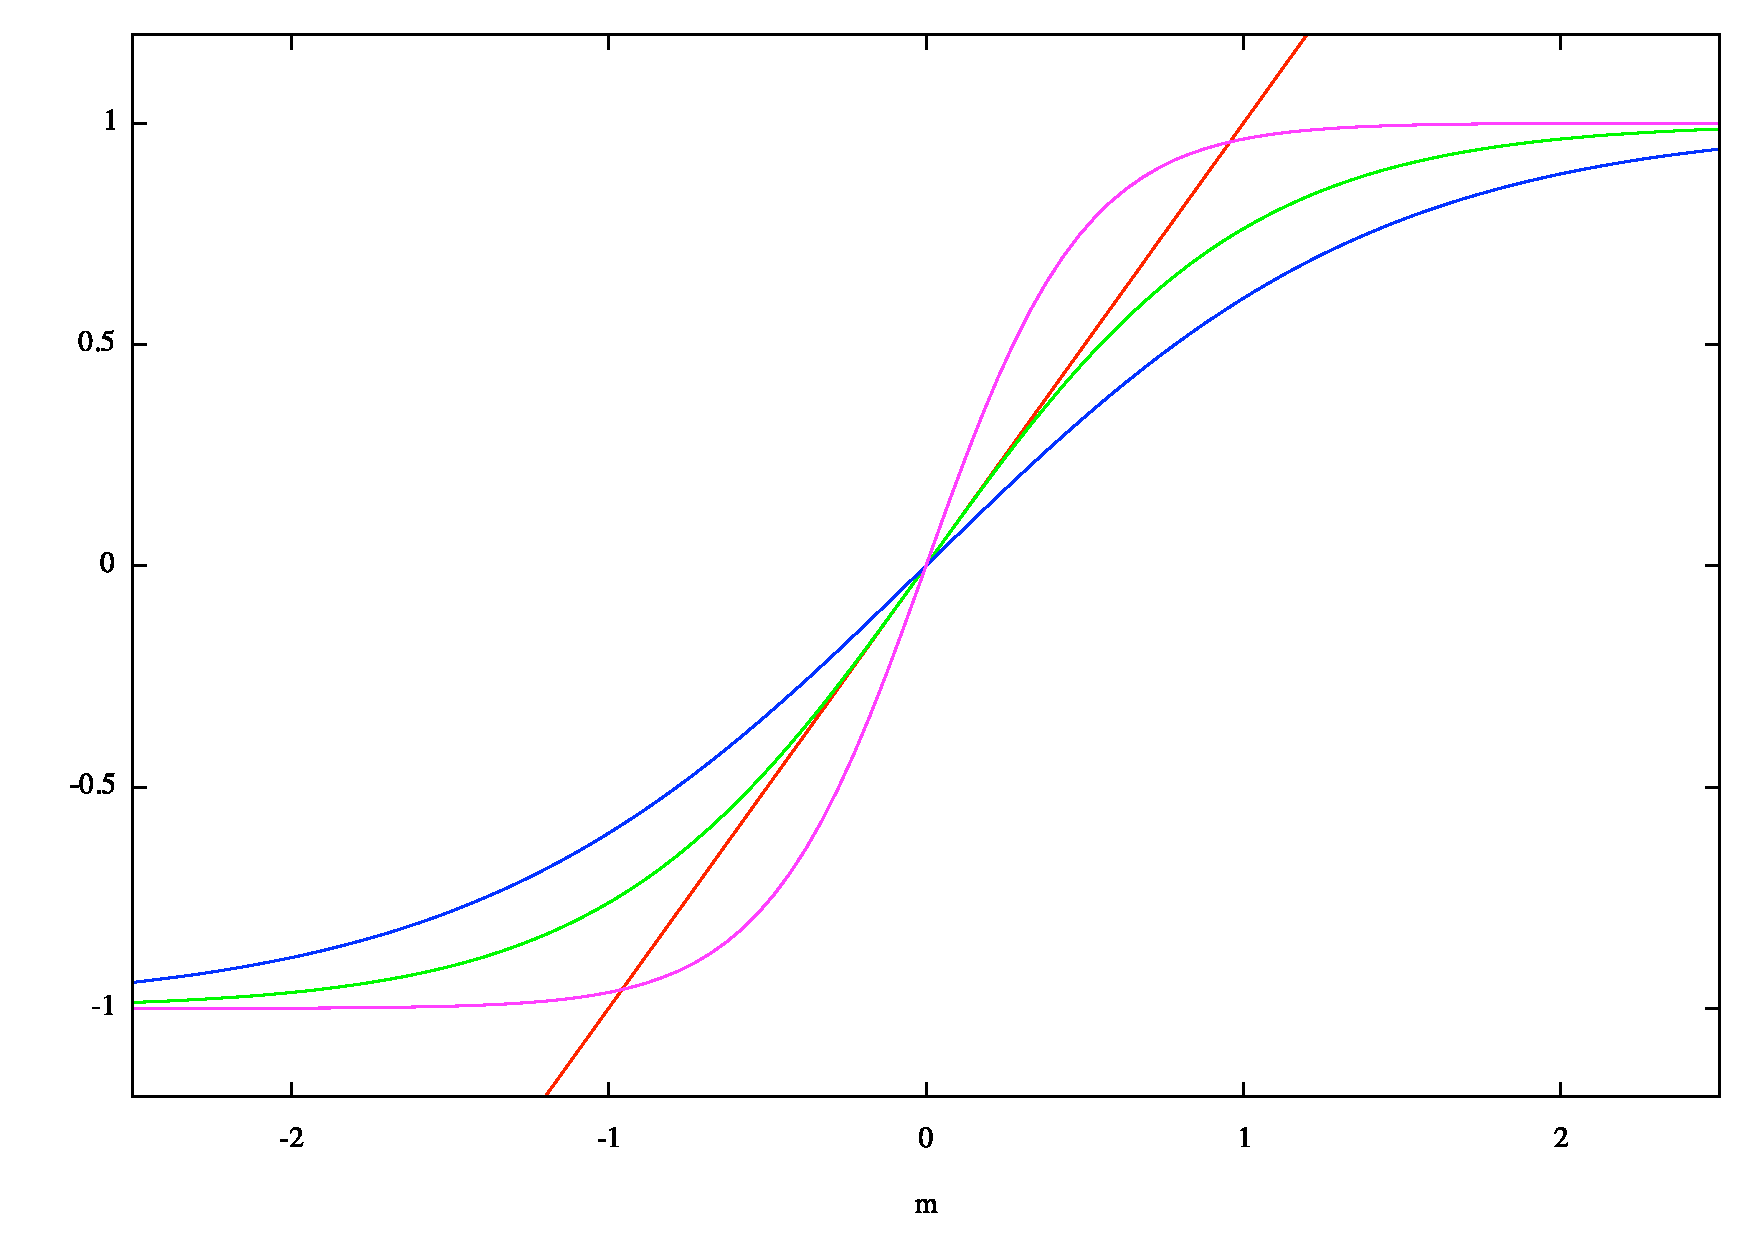
\includegraphics[width=0.75\textwidth]{mf.pdf}
\caption{Soluzione grafica dell'equazione di campo medio. La curva verde è la
tangente iperbolica calcolata per $\beta = \beta_{c}$.}
  \label{fig:mf}
\end{figure}
%%%

Ora, se $1/2D\beta > 1$ la derivata seconda di $\phi$ è sempre maggiore di zero,perché $m^{2}$ è sempre minore di $1$, quindi $m=0$ costituisce un minimo ed è
l'unica soluzione dell'equazione di campo medio. Invece se $1/2D\beta < 1$
allora $m=0$ è un massimo, e compaiono altre soluzioni. In Figura \ref{fig:mf}
c'è la visualizzazione grafica delle possibili soluzioni.

Appare dunque chiaro che $\beta_{c}\equiv 1/2D$ rappresenta un valore {\em
critico} di $\beta$; per valori di $\beta$ minori di $\beta_{c}$ (ovvero per
valori di $T > T_{c}$) il sistema non presenta magnetizzazione spontanea, che sisviluppa invece per valori della temperatura inferiori a quella critica.

Calcoliamo la magnetizzazione spontanea $m_{s}$ nel limite $T\to 0$, che
equivale a $\beta\to\infty$. In questo caso possiamo scrivere
%---
\be
\tanh(2D\beta m) \simeq 1 - 2e^{-4D\beta m}
\ee
%---
La magnetizzazione spontanea è dunque uguale a $1$ a meno di correzioni
esponenziali:
%---
\be
m_{s} \simeq \pm(1 - 2e^{-4D\beta})
\ee
%---
Invece per $T\to T_{c}^{-}$, ossia per $2D\beta\to 1^{+}$, sappiamo che la
magnetizzazione sarà vicina a zero, e questo ci permette di espandere la
tangente iperbolica:
%---
\be
m_{s} \simeq 2D\beta m_{s} - \frac{8D^{3}\beta^{3}m_{s}^{3}}{3}
\ee
%---
Vediamo però che $8D^{3}\beta^{3} = (\beta/\beta_{c})^{3}$, e dunque a
quest'ordine può essere trascurato: otteniamo quindi
%---
\be
m_{s}\propto(T_{c}-T)^{1/2}
\ee
%---
Per quel che riguarda la densità di energia interna, abbiamo $u = -Dm^{2}$.
Dunque per $T>T_{c}$ l'energia interna è nulla, mentre l'andamento critico al disotto di $T_{c}$ è chiaramente
%---
\be
u\propto(T_{c}-T)^{1}
\ee
%---
Il fatto che $u$ non sia discontinuo alla transizione implica che la transizionestessa non è del primo ordine (non c'è calore latente).
Se $T=T_{c}$ e $h\ne 0$ (ma piccolo in valore assoluto) abbiamo
%---
\be
m = \tanh(m+h) \simeq m + h - m^{3}/3
\ee
%---
(nella quale abbiamo trascurato un termine $O(h^{3})$), e otteniamo quindi
%---
\be
m \propto h^{1/3}
\ee
%---
Va notato che l'approssimazione di campo medio prevede una transizione di fase
anche in $D=1$, cosa che sappiamo essere falsa.

\subsection{Un modello esattamente risolubile}

La soluzione esatta del modello di Ising in $D=2$ e le soluzioni numeriche in
$D=3$ e in dimensioni superiori mostrano che l'approssimazione di campo medio
diventa sempre migliore al crescere di $D$. Questo risultato è intuitivamente
corretto: al crescere di $D$ cresce il numero di primi vicini di un determinato
spin (il numero di coordinazione di un reticolo semplicemente cubico è pari a
$2D$), e quindi è ragionevole supporre che l'approssimazione di campo medio, chesi basa proprio sul fatto che la magnetizzazione locale è data dal ``campo
medio'' dei primi vicini, migliori al crescere del numero di siti reticolari coni quali un dato spin interagisce direttamente.

Per rendere più concreta questa affermazione utilizziamo un modello esattamente
risolubile. L'Hamiltoniana è uguale a quella di Ising, ma ogni spin interagisce
con tutti gli altri spin del reticolo. Allo stesso tempo l'accoppiamento $J$
descresce con $N$, il numero di spin totali. Abbiamo dunque
%---
\be
e^{-\beta\Ham} = \exp\left(\frac{\beta}{2N}\sum_{i,j}\sigma_{i}\sigma_{j} +
\beta h\sum_{i}\sigma_{i} \right)
\ee
%---
in cui il fattore $2$ ci permette di sommare due volte su tutti gli spin. La
peculiarità di questo modello è che il fattore di Boltzmann può essere espresso
come un integrale gaussiano:
%---
\be
e^{-\beta\Ham} =
\left(\frac{N\beta}{2\pi}\right)^{1/2}\int_{-\infty}^{\infty}\de{\lambda}\,\exp\left(
-\frac{N\beta\lambda^{2}}{2} +\sum_{i}(\beta\lambda + \beta h)\sigma_{i}\right)
\ee
%---
e possiamo quindi scrivere
%---
\be
Q = \sum_{[\sigma]}e^{-\beta\Ham} =
\left(\frac{N\beta}{2\pi}\right)^{1/2}\int_{-\infty}^{\infty}\de{\lambda}\,\exp\left(-\frac{N\beta\lambda^{2}}{2}\right)
\sum_{[\sigma]}
\prod_{i}\exp\left((\beta\lambda + \beta h)\sigma_{i}\right)
\ee
%---
Invertendo la somma sulle configurazioni con la produttoria su tutti i siti,
otteniamo
%---
\be
Q =
\left(\frac{N\beta}{2\pi}\right)^{1/2}\int_{-\infty}^{\infty}\de{\lambda}\,\exp\left(-\frac{N\beta\lambda^{2}}{2}\right)\left\{
2\cosh[\beta(\lambda+h)]\right\}^{N}
\ee
%---
e in definitiva
%---
\be
Q =
\left(\frac{N\beta}{2\pi}\right)^{1/2}\int_{-\infty}^{\infty}\de{\lambda}\,e^{N\beta
B(\lambda)}
\ee
%---
in cui
%---
\be
B(\lambda) = -\frac{\lambda^{2}}{2} +
\frac{1}{\beta}\ln\{2\cosh[\beta(\lambda+h)]\}
\ee
%---
Il metodo dello {\em steepest descent} ci dice che
%---
\be
\lim_{N\to\infty} \frac{1}{N}\ln\left\{
\int_{-\infty}^{\infty}\de{x}\,e^{Ng(x)}\right\} = \max_{x}\{g(x)\} + O(N^{-1})
\ee
%---
e per la densità di energia libera otteniamo proprio
%---
\be
f = \frac{A}{N} = -\frac{1}{N\beta}\ln Q
\ee
%---
Dunque per calcolare $f$ nel limite termodinamico sarà sufficiente calcolare il
massimo della funzione $B(\lambda)$. Si ottiene facilmente che il valore di
$\lambda$ che massimizza la funzione $B(\lambda)$ soddisfa l'equazione
%---
\be
\bar{\lambda} = \tanh(\beta h +\beta\bar{\lambda})
\ee
%---
e ci chiediamo ora qual è il significato fisico di $\bar\lambda$. Calcoliamo la
magnetizzazione del sistema:
%---
\be
f = -\frac{B(\bar\lambda)}{\beta}\quad\quad m = -\dpar{f}{h}
\ee
%---
e si trova facilmente
%---
\be
m = \frac{1}{\beta}\dpar{B(\bar\lambda)}{h} = \tanh(\beta h
+\beta\bar{\lambda})\ee
%---
e dunque $\bar{\lambda} = m$. Quindi in questo caso l'equazione di campo medio
risolve esattamente il modello.

\appendix
%%%%%%%%%%%%%%%%%%%%%%%%%%%%%%%%%%%%%%%%%%%%%%%%%%%%%%%%%%%%%%%%%%%%%%%%
\chapter{Appendice matemarica}
\label{app:matematica}
%%%%%%%%%%%%%%%%%%%%%%%%%%%%%%%%%%%%%%%%%%%%%%%%%%%%%%%%%%%%%%%%%%%%%%%%

%%%%%%%%%%%%%%%%%%%%%%%%%%%%%%%%%%%%%%%%%%%%%%%%%%%%%%%%%%%%%%%%%%%%%%%%
\section{Alcune funzioni e formule utili}
%%%%%%%%%%%%%%%%%%%%%%%%%%%%%%%%%%%%%%%%%%%%%%%%%%%%%%%%%%%%%%%%%%%%%%%%

%%%%%%%%%%%%%%%%%%%%%%%%%%%%%%%%%%%%%%%%%%%%%%%%%%%%%%%%%%%%%%%%%%%%%%%%
\subsection{La funzione $\Gamma$}
\label{subsec:app1-gamma}
%%%%%%%%%%%%%%%%%%%%%%%%%%%%%%%%%%%%%%%%%%%%%%%%%%%%%%%%%%%%%%%%%%%%%%%%

La funzione $\Gamma$ di Eulero è definita da:
\be
\label{eq:defGamma}
\Gamma(\nu) = \int_0^\infty\de{x} \, e^{-x} \, x^{\nu-1} \quad\quad \nu > 0
\ee
Notiamo subito che
\be
\Gamma(1) = 1
\ee
Integrando per parti la (\ref{eq:defGamma}) otteniamo l'equazione di ricorrenza
\be
\Gamma(\nu+1) = \nu \Gamma(\nu)
\ee
Dalla precedente ricaviamo subito
\be
\Gamma(\nu+1) = \nu(\nu-1)(\nu-2) \, \cdots \, (1+p) p \, \Gamma(p) \quad\quad 0 < p \le 1
\ee
nella quale $p$ è la parte frazionaria di $\nu$. Se $\nu$ è intero abbiamo l'identificazione
\be
\Gamma(n+1) = n!
\ee
mentre se è semintero otteniamo
\bea
\label{eq:GammaSemint}
\Gamma \left( m + \dfrac{1}{2} \right) &\equiv& \left( m - \dfrac{1}{2} \right)! =
\left( m - \dfrac{1}{2} \right) \left( m - \dfrac{3}{2} \right) \, \cdots \, 
\left( \dfrac{1}{2} \right) \Gamma\left( \dfrac{1}{2} \right) \nonumber \\
&=& \dfrac{(2m-1)(2m-3) \, \cdots \, 1}{2^m}\pi^{1/2}
\eea
nella quale abbiamo sfruttato il fatto che
\be
\label{eq:Gamma12}
\Gamma \left( \dfrac{1}{2} \right) = \pi^{1/2}
\ee

\noindent
Cambiando variabile, $x = \alpha y^2$, possiamo scrivere la (\ref{eq:defGamma}) come
\be
\Gamma(\nu) = 2\alpha^\nu \int_0^\infty \de{y} \, e^{-\alpha y^2} \, y^{2\nu-1}
\ee
e ponendo $\mu = 2\nu - 1$ possiamo calcolare gli integrali notevoli
\be
I_\mu(\alpha) \equiv \int_0^\infty \de{y} \, e^{-\alpha y^2} \, y^{\mu}
= \dfrac{1}{2\alpha^{(\mu+1)/2}}\Gamma \left( \dfrac{\mu+1}{2} \right)
\ee

\noindent
Anche gli integrali appena definiti soddisfano una relazione di ricorrenza:
\be
I_{\mu+2}(\alpha) = -\dfrac{\text{d}}{\de{\alpha}} I_\mu(\alpha)
\ee
Per $\mu$ pari abbiamo, per esempio,
\be
I_0(\alpha) = \dfrac{1}{2}\left( \dfrac{\pi}{\alpha}   \right)^{1/2} \quad
I_2(\alpha) = \dfrac{1}{4}\left( \dfrac{\pi}{\alpha^3} \right)^{1/2} \quad
I_4(\alpha) = \dfrac{3}{8}\left( \dfrac{\pi}{\alpha^5} \right)^{1/2}
\ee
mentre per $\mu$ dispari
\be
I_1(\alpha) = \dfrac{1}{2\alpha}   \quad
I_3(\alpha) = \dfrac{1}{2\alpha^2} \quad
I_5(\alpha) = \dfrac{1}{\alpha^3}
\ee
Notiamo infine che abbiamo
\be
\int_{-\infty}^\infty \de{y} \, e^{-\alpha y^2} \, y^{\mu} = 
\left\{
\begin{array}{ll}
2I_\mu(\alpha) & \quad \text{se\ } \mu \text{\ è pari} \\
0              & \quad \text{altrimenti}
\end{array}
\right.
\ee

%%%%%%%%%%%%%%%%%%%%%%%%%%%%%%%%%%%%%%%%%%%%%%%%%%%%%%%%%%%%%%%%%%%%%%%%
\subsection{La formula di Stirling}
\label{subsec:app1-stirling}
%%%%%%%%%%%%%%%%%%%%%%%%%%%%%%%%%%%%%%%%%%%%%%%%%%%%%%%%%%%%%%%%%%%%%%%%

La formula di Stirling può essere ottenuta applicando la formula di Eulero--Maclaurin. Per definizione abbiamo
\be
\ln\left(\, n! \,\right) = \sum_{k=1}^{n} \ln k
\ee
e sostituendo l'integrale alla somma possiamo scrivere
\be
\ln\left(\, n! \,\right) \simeq \int_1^n \de{x} \, \ln x
= \big[x\ln x - x \big]_1^n \simeq n\ln n - n
\ee

%%%%%%%%%%%%%%%%%%%%%%%%%%%%%%%%%%%%%%%%%%%%%%%%%%%%%%%%%%%%%%%%%%%%%%%%
\subsection{Il teorema multinomiale}
\label{subsec:app1-multinomiale}
%%%%%%%%%%%%%%%%%%%%%%%%%%%%%%%%%%%%%%%%%%%%%%%%%%%%%%%%%%%%%%%%%%%%%%%%

È un'estensione del teorema binomiale. Dato un set di interi $\seti{k_i}$ con $i = 1, 2, \dots, n$ che soddisfano il vincolo
\be
\sum_{i=1}^n k_i = N
\ee 
si può dimostrare che
\be
\sum_{\seti{k_i}}\left[
N!\prod_{i=1}^n \dfrac{x_i^{k_i}}{k_i!}
\right] = (x_1 + x_2 + \cdots + x_n)^N
\ee
\end{document}
